\documentclass[12pt]{report}

\usepackage{Dedman-Thesis-Latex-Template/sty/DL_thesis}  % Global Style for particular SMU College, e.g. DL_thesis.sty

% \usepackage{DL_thesis_v2016}
\usepackage{adjustbox}       % TCM Extends the graphicx package to do trimming and other adjustments.
\usepackage{algorithm}       % TCM Algorithm block See http://algorithms.berlios.de/
\usepackage{algorithmic}     % TCM Algorithm & Peudocode See http://en.wikibooks.org/wiki/LaTeX/Algorithms_and_Pseudocode
\usepackage{amsmath}         % Need for subequations
\usepackage{mathrsfs} %https://ctan.org/pkg/mathrsfs
%\usepackage{amssymb}        % amssymb-telda and math symbols
\usepackage{booktabs}        % TCM Allows fancy Tables
\usepackage{boxedminipage}   % Boxes around figures
\usepackage{breqn}           % TCM Automatically breaks long equation lines - usually
\usepackage{changepage} 	 % TCM Allows one to temporarily change right and left margins
\usepackage{cite} 	 		 % TCM Allows improved handling of numeric citations including automatic ordering and ranges of multiple cites
\usepackage{enumitem} 		 % TCM Allows one to easily change the labels for enumerate list
%\usepackage{epsf}           % TCM This EPS file package is greatly depreciated for the graphicx package bundle. Use at own risk.
\usepackage{fancyhdr}
\usepackage{flafter}         % Floats should always appear after their definition
\usepackage[flushleft]{threeparttable}  % TCM This package allows for notes under tables.  Flushleft option flushes the note left margin of table (center is default)
\usepackage{geometry}		 % TCM Allows to customize paper size and margins.
\usepackage{graphicx}        % TCM Extends graphics package for figures. Provides op­tional ar­gu­ments to the \in­clude­graph­ics com­mand
\usepackage{epstopdf}        % TCM Converts eps images to PDF to use in graphicx package.  Must be loaded after graphicx package
\usepackage{longtable}       % TCM Allows for Automatic page breaks for long tables
%\usepackage{jneurosci}       % TCM The jneurosci bibliography style makes use of some commands - for example, \citeauthoryear.  Must include if using named or acmsmall bib style
\usepackage{ltablex}		 % TCM Modifies Tabularx Package by combining properties of tabularx and longtable.
\usepackage[maxfloats=36]{morefloats}      % Latex will handle more floats 18-36
\usepackage{moresize}        % TCM Adds \HUGE and \ssmall font sizes
\usepackage{multirow}        % TCM Allows multirow cells in tables (similar to merge and center in Excel)
%\usepackage{named}           % TCM Bibliography style that allows for more fine-tuned citing. Commands include \cite, \citeauthor, \citeyear and \shortcite (for after you've already used \citeauthor).
\usepackage{outlines}		 % TCM Needed for outlines
\usepackage{rotate}			 % TCM Performs rotations of floating environments (images w/ cations, etc)
\usepackage{rotating}        % Need for sidewaystable
\usepackage{scrextend}		 % TCM package that allows for KOMA-Script classes available for other classes: e.g., labeling lists etc.  See package documentation for further information.
\usepackage{pdflscape}		 % TCM Allows Landscape Page
%%\usepackage{qtree}         % Need for trees
\usepackage{setspace}        % TCM Allows for more intuitive commands for single and double spacing
\usepackage{siunitx}		 % TCM package required to ensure units are typeset properly with numbers e.g. \SI{10}{\kg\m\per\square\s}
\sisetup{output-exponent-marker=\ensuremath{\mathrm{E}}}  % TCM Option allows for Scientific notation of Numbers.  Format is \num{#.####E##}
% \usepackage[superscript]{cite}		  % TCM Makes citations superscript instead of [#]
\usepackage [table]{xcolor}	 % TCM Allows coloring of tables
\usepackage{tabularx}		 % TCM Package which allows paragraphs in Tables
% \usepackage{thumbpdf}		  % TCM Comment out as causes warnings, can easily create thumbs in Adobe if needed.

%===========================================================
%  Color ToDo Comment Notes for editing
%===========================================================
\usepackage[colorinlistoftodos,textwidth=25mm,shadow,backgroundcolor=green]{todonotes}				  % TCM Allows margin comments
\usepackage{marginnote}				  % TCM Require for Todonotes in Align Envionment
%~~~~~~~~~~~~~~~~~~~~~~~~~~~~~~~~~~~~~~~~~~~~~~~~~~~~~~~~~~~
% TCM  BEGIN Altering Todonotes Commands to use Marginnote instead of Marginpar to use todonotes in align environment
%~~~~~~~~~~~~~~~~~~~~~~~~~~~~~~~~~~~~~~~~~~~~~~~~~~~~~~~~~~~
\makeatletter
\renewcommand{\@todonotes@drawMarginNoteWithLine}{%
 \begin{tikzpicture}[remember picture, overlay, baseline=-0.75ex]%
  \node [coordinate] (inText) {};%
 \end{tikzpicture}%
 \marginnote[{% Draw note in left margin
  \@todonotes@drawMarginNote%
  \@todonotes@drawLineToLeftMargin%
  }]{% Draw note in right margin
  \@todonotes@drawMarginNote%
  \@todonotes@drawLineToRightMargin%
 }%
}
\makeatother
%----------------------------------------------------
% TCM  BEGIN New Todonotes Command to use single line spacing (sls) in note
%----------------------------------------------------
\newcommand{\slstodo}[2][]
{\todo[caption={#2}, size=\small, #1]{\renewcommand{\baselinestretch}{0.5}\selectfont#2\par}}
%----------------------------------------------------
% TCM  END New Todonotes Command to use single spacing in note
%----------------------------------------------------

%~~~~~~~~~~~~~~~~~~~~~~~~~~~~~~~~~~~~~~~~~~~~~~~~~~~~~~~~~~~
% TCM  END Altering Todonotes Commands to use Marginnote instead of Marginpar to use todonotes in align
%~~~~~~~~~~~~~~~~~~~~~~~~~~~~~~~~~~~~~~~~~~~~~~~~~~~~~~~~~~~

\usepackage{verbatim}        % TCM Verbatim text block
\usepackage{wrapfig}         % Wrap figures
\usepackage{xspace}          % Allows dynamic space in global text variables. This can allow you to just use \newCommandName rather than \newCommandName{}.
\usepackage [bookmarks=true,backref=page, hyperfigures=true, pdfpagelabels=false] {hyperref}
\hypersetup{
 % TCM Added more precise definition and options for Hyperref package.
 % TCM Comment out or change hyperref preferences
 % TCM \hypersetup should be loaded last
 bookmarksopen=true,				  % True: Open bookmark tree
 bookmarksnumbered=true, 		  % True: put section numbers in bookmarks
 breaklinks=true,				  % True: split the url over multiple lines
 %    draft=true,						  % True: do not do any hyper linking
 filecolor=magenta, 				  % Color of file links
 citecolor=blue, 				  % Color of links to bibliography
 colorlinks=true, 				  % False: boxed links; true: colored links
 linkcolor=blue, 				  % Color of internal links
 linktocpage=true, 				  % True: Makes the page number of TOC the link vs the text
 %    pagebackref=true,				  % True: Links references back to referring page
 pdfnewwindow=true,         		  % True: URL links in new window
 plainpages=false, 				  % True: do page number anchors as plain Arabic
 pdffitwindow=false,        		  % Window fit to page when opened
 pdfmenubar=true,           		  % Show Acrobat menu
 pdfstartview={FitH},       		  % Fits the width of the page to the window
 pdftoolbar=true, 				  % Show Acrobat toolbar
 pdfauthor={Author}, 			  % Author in PDF document properties
 pdfcreator={Author}, 			  % Creator of the document in PDF document properties
 pdfkeywords={Keyword1} {Keyword2} {Keyword3} {Keyword4} {Author}, % List of keywords in PDF document properties
 pdfproducer={Producer}, 		  % Producer of the document in PDF document properties
 pdfsubject={Subject},   % Subject of the document in PDF document properties
 pdftitle={Title of Dissertation}, % Title in PDF document properties
 unicode=false,             		  % Non-Latin characters in Acrobat bookmarks
 urlcolor=cyan 					  % Color of external links
}
\usepackage{bookmark}		 		  % TCM Eliminates Warning Bookmark level greater than one.  Must be loaded after Hyperref

% Load additional packages here.
% Be careful of the loading order with respect to packages.tex as conflicts can easily arise.
% This is not a part of the base template and so will never be overwritten during updates.
\usepackage{slashed}% https://www.ctan.org/pkg/slashed
\usepackage{braket}% https://www.ctan.org/pkg/braket
 % Uncomment to load additional user required packages
\usepackage{graphicx} % For images
\graphicspath{{Images/}}
\usepackage{float}		% For tables and other floats
\usepackage{verbatim} 	% For comments and other
\usepackage{amsmath}  	% For math
\usepackage{amssymb}  	% For more math
\usepackage{fullpage} 	% Set margins and place page numbers at bottom center
\usepackage{listings} 	% For source code
\usepackage{subfig}   	% For subfigures
\usepackage[usenames,dvipsnames]{xcolor}	% For colors and names for color boxed links
%\usepackage[usenames,dvipsnames]{color}	% For colors and names
\usepackage[]{hyperref}           		% For hyperlinks and indexing the PDF
\hypersetup{
 colorlinks=false,		% Surround the links by color frames (false) or colors the text of the links (true)
 citecolor=blue,		% Color of citation links
 filecolor=black,		% Color of file links
 linkcolor=red,		% Color of internal links (sections, pages, etc.)
 urlcolor=black,		% Color of url hyperlinks
 linkbordercolor=red, 	% Color of links to bibliography
 citebordercolor=blue,	% Color of file links
 urlbordercolor=blue	% Color of external links
}
\usepackage{calligra}	% For generating 'script r'
\DeclareMathAlphabet{\mathcalligra}{T1}{calligra}{m}{n}
%\DeclareFontShape{T1}{calligra}{m}{n}{<->s*[2.2]callig15}{}
\usepackage{mathrsfs}	% For nice math calligraphy fonts
\usepackage{custom}
\usepackage{HEP}		% High energy physics commands
%\usepackage{draftmode}		% Draft mode edit;	Remember to remove the linenumbers command
\usepackage{soul}			% Allows strikethrough of text with \st{text}
\usepackage{cancel}		% Allows for \cancelto{cancel_to_value}{quantity_being_canceled}
\usepackage{mathtools}	% Needed for mathclap
% \usepackage{tabu}
\usepackage{booktabs}

%%%%% CIRCUITS %%%%%
\usepackage{pgfplots}
\usepackage{tikz}%
\usepackage{tkz-euclide}
%\usepackage[siunitx]{circuitikz}
\usetikzlibrary{decorations.markings}
\usetikzlibrary{patterns}
%%%%%%%%%%%%%%%%
\usepackage{3dplot} %requires 3dplot.sty to be in same directory, or in your LaTeX installation

%\usepackage{al?phalph}
\renewcommand\vec[1]{\ensuremath\boldsymbol{#1}}	% Makes vectors boldface type, replaces arrows.
\renewcommand{\thefootnote}{\fnsymbol{footnote}}		% Causes footnotes to be indicated symbols, not numbers
%\numberwithin{equation}{section}					% Labels equations due to their section number
\hyphenation{ATLAS}							% Defines where words may be hyphenated

%All custom made commands are located in custom.sty in ~/Library/texlive/2010/texmf-var/tex/latex/

% Redefine the itemize symbol to be empty space for problem 3.
%\renewcommand*\labelitemi{}

% Box matrix shortcuts
\newcommand{\bbx}{\begin{bmatrix}}
\newcommand{\ebx}{\end{bmatrix}}
\newcommand{\ba}{\begin{array}}
\newcommand{\ea}{\end{array}}
\newcommand{\nin}{\noindent}

% Change enumerate bullet point
\usepackage{enumerate}

\usepackage{afterpage}
\newcommand\blankpage{%
 \null
 %   \thispagestyle{empty}%
 %   \addtocounter{page}{-1}%
 \newpage}


\usepackage{caption}
\usepackage{empheq}

\usepackage{pdfpages}

\usepackage{listings}


%======================================================================
% Custom Commands  Inital Creation TCM 2015
%======================================================================
% Use this document to place all of your global new commands
%======================================================================

%======================================================================
% BEGIN SMU Custom Commands
%======================================================================
% The many of the following commands were originally in the smu_thesis.sty
% file. Commands and comments were moved here to make style file more about
% document style. While custom environments can technically be considered
% style, the student created environments are included here to simplify
% the style file. Often these commands were created by students over the
% years and placed in the style file.  The commands have not been
% verified and can be obsolete LaTeX commands. The Commands can be used
% or ignored.
%======================================================================
%----------------------------------------------------------------------
% BEGIN TCM Commands to set formatting for Paragraph section to have line
%           feed after heading & Numbered. This custom command makes
%           \paragraph, in essence, a form of \subsubsubsection.
%           Uncomment to use.
%----------------------------------------------------------------------
%  \makeatletter
%  \renewcommand\paragraph{\@startsection{paragraph}{4}{\z@}%
%    {-3.25ex\@plus -1ex \@minus -.2ex}%
%    {1.5ex \@plus .2ex}%
%    {\normalfont\normalsize\bfseries}}
%  \makeatother
%----------------------------------------------------------------------
% END of Commands to set formatting for Paragraph section to have line
%       feed after heading TCM
%----------------------------------------------------------------------

% eliminate compile warnings for noindent hfill hbox in PDF bookmarks
\pdfstringdefDisableCommands{
 \def\hbox{ }% hyperref (temporarily) changes \hbox to a space in this context.
 \def\hfill{ }% hyperref (temporarily) changes \hfill to a space in this context.
 \def\noindent{ }% hyperref (temporarily) changes \noindent to a space in this context.
 \def\hskip{ }% hyperref (temporarily) changes \hskip to a space in this context.
}

%----------------------------------------------------------------------
% BEGIN Shortcuts to insert calligraphic letters in Math Mode Only
%----------------------------------------------------------------------
\newcommand{\cA}{{\mathcal A}}
\newcommand{\cB}{{\mathcal B}}
\newcommand{\cC}{{\mathcal C}}
\newcommand{\cD}{{\mathcal D}}
\newcommand{\cE}{{\mathcal E}}
\newcommand{\cF}{{\mathcal F}}
\newcommand{\cG}{{\mathcal G}}
\newcommand{\cH}{{\mathcal H}}
\newcommand{\cI}{{\mathcal I}}
\newcommand{\cJ}{{\mathcal J}}
\newcommand{\cK}{{\mathcal K}}
\newcommand{\cL}{{\mathcal L}}
\newcommand{\cM}{{\mathcal M}}
\newcommand{\cN}{{\mathcal N}}
\newcommand{\cO}{{\mathcal O}}
\newcommand{\cP}{{\mathcal P}}
\newcommand{\cQ}{{\mathcal Q}}
\newcommand{\cR}{{\mathcal R}}
\newcommand{\cS}{{\mathcal S}}
\newcommand{\cT}{{\mathcal T}}
\newcommand{\cU}{{\mathcal U}}
\newcommand{\cV}{{\mathcal V}}
\newcommand{\cW}{{\mathcal W}}
\newcommand{\cX}{{\mathcal X}}
\newcommand{\cY}{{\mathcal Y}}
\newcommand{\cZ}{{\mathcal Z}}
% Lower case caligraphy letters
\newcommand{\cw}{{\mathcal w}}
%----------------------------------------------------------------------
% END Shortcuts to insert calligraphic letters in Math Mode Only
%----------------------------------------------------------------------
%----------------------------------------------------------------------
% BEGIN Shortcuts to insert boldface letters
%----------------------------------------------------------------------
\newcommand{\bA}{{\bf A}}
\newcommand{\bB}{{\bf B}}
\newcommand{\bC}{{\bf C}}
\newcommand{\bD}{{\bf D}}
\newcommand{\bE}{{\bf E}}
\newcommand{\bF}{{\bf F}}
\newcommand{\bG}{{\bf G}}
\newcommand{\bH}{{\bf H}}
\newcommand{\bI}{{\bf I}}
\newcommand{\bJ}{{\bf J}}
\newcommand{\bK}{{\bf K}}
\newcommand{\bL}{{\bf L}}
\newcommand{\bM}{{\bf M}}
\newcommand{\bN}{{\bf N}}
\newcommand{\bO}{{\bf O}}
\newcommand{\bP}{{\bf P}}
\newcommand{\bQ}{{\bf Q}}
\newcommand{\bR}{{\bf R}}
\newcommand{\bS}{{\bf S}}
\newcommand{\bT}{{\bf T}}
\newcommand{\bU}{{\bf U}}
\newcommand{\bV}{{\bf V}}
\newcommand{\bW}{{\bf W}}
\newcommand{\bX}{{\bf X}}
\newcommand{\bY}{{\bf Y}}
\newcommand{\bZ}{{\bf Z}}
%----------------------------------------------------------------------
% END Shortcuts to insert boldface letters
%----------------------------------------------------------------------
%----------------------------------------------------------------------
% BEGIN Shortcuts to insert overline symbols in Math Mode Only
%----------------------------------------------------------------------
\newcommand{\oA}{{\overline A}}
\newcommand{\oB}{{\overline B}}
\newcommand{\oC}{{\overline C}}
\newcommand{\oD}{{\overline D}}
\newcommand{\oE}{{\overline E}}
\newcommand{\oF}{{\overline F}}
\newcommand{\oG}{{\overline G}}
\newcommand{\oH}{{\overline H}}
\newcommand{\oI}{{\overline I}}
\newcommand{\oJ}{{\overline J}}
\newcommand{\oK}{{\overline K}}
\newcommand{\oL}{{\overline L}}
\newcommand{\oM}{{\overline M}}
\newcommand{\oN}{{\overline N}}
\newcommand{\oO}{{\overline O}}
\newcommand{\oP}{{\overline P}}
\newcommand{\oQ}{{\overline Q}}
\newcommand{\oR}{{\overline R}}
\newcommand{\oS}{{\overline S}}
\newcommand{\oT}{{\overline T}}
\newcommand{\oU}{{\overline U}}
\newcommand{\oV}{{\overline V}}
\newcommand{\oW}{{\overline W}}
\newcommand{\oX}{{\overline X}}
\newcommand{\oY}{{\overline Y}}
\newcommand{\oZ}{{\overline Z}}
% Lower case overline
\newcommand{\ovd}{{\overline d}}
\newcommand{\ove}{{\overline e}}
\newcommand{\ovf}{{\overline f}}
\newcommand{\ovg}{{\overline g}}
\newcommand{\ovh}{{\overline h}}
\newcommand{\ovi}{{\overline i}}
%----------------------------------------------------------------------
% END Shortcuts to insert overline symbols in Math Mode Only
%----------------------------------------------------------------------
%----------------------------------------------------------------------
% BEGIN Shortcuts to insert vector symbols in Math Mode Only
%----------------------------------------------------------------------
\newcommand{\vS}{{\vec S}}
\newcommand{\vT}{{\vec T}}
\newcommand{\vU}{{\vec U}}
\newcommand{\vV}{{\vec V}}
\newcommand{\vW}{{\vec W}}
\newcommand{\vX}{{\vec X}}
\newcommand{\vY}{{\vec Y}}
\newcommand{\vZ}{{\vec Z}}
% Lower case vectors
\newcommand{\vs}{{\vec s}}
\newcommand{\vt}{{\vec t}}
\newcommand{\vu}{{\vec u}}
\newcommand{\vv}{{\vec v}}
\newcommand{\vw}{{\vec w}}
\newcommand{\vx}{{\vec x}}
%----------------------------------------------------------------------
% END Shortcuts to insert vector symbols in Math Mode Only
%----------------------------------------------------------------------
%----------------------------------------------------------------------
% BEGIN Misc. Commands defined by students
%----------------------------------------------------------------------
\newcommand{\myqed}{\vspace{-1.1cm} \qed \vspace{0.9cm}}
\newcommand{\qed}{\mbox{$\ \Box$}}
\newcommand{\lqed}{\qed\vspace{.1in}}
\newcommand{\nf}{{\mbox{$\sim$}}}
\newcommand{\wt}{\mbox{$\widehat{T}$}}
\newcommand{\as}{\mbox{$/\hspace{-2mm}>$}}
\newcommand{\equi}{\mbox{$\leftrightarrow$}}
\newcommand{\myeq}{\mbox{$\leftrightarrow$}}
%\newcommand{\tab}{\hspace*{4em}}
%\newcommand{\ind}{\hspace*{2em}}
%\newcommand{\mif}{\mbox{ :- }}
%\newcommand{\dd}{\mbox{$\bullet$}}
\newcommand{\dd}{\mbox{\ $\mid$\ }}

\newcommand{\ind}{\hspace*{2.0em}}
\newcommand{\tab}{\hspace*{4em}}

\newcommand{\myp}{\protect{$+$}}
\newcommand{\mypp}[1]{\protect{${#1}$}}
\newcommand{\myf}[2]{\protect{\ \(\frac{\mbox{\rm #1}}{\mbox{\rm #2}}\)}\ }
\newcommand{\myup}{\protect{$ \uparrow$}}
\newcommand{\scc}[1]{\protect{\ \ \ $ SCC = {#1} $}}

\newcommand{\twoheadrightarrow}{{\rightarrow \hspace{-0.3cm} \rightarrow \hspace{0.2cm}}}

\newcommand{\chap}[1]{\chapter{\protect{\bf {#1}}}}
\newcommand{\mytab}{\hspace*{13em}}
\newcommand{\bleft}{\left \{\ }
\newcommand{\bright}{\ \right \}}
\newcommand{\sind}{ \ \ \ }
\newcommand{\mand}{ \ \&\ }
\newcommand{\mif}{\mbox{\ :-\ }}
%%%\newcommand{\nf}{\sim}
\newcommand{\posI}{$I^+$}
\newcommand{\negI}{$I^-$}
%\newcommand{\AST}{$AST(P)$}
\newcommand{\Ip}[1]{${\mathcal I}_{#1}$}
\newcommand{\II}[1]{${\mathcal I}({#1})$}
%\newcommand{\HU}[1]{${\mathcal HU}_{#1}$}
%\newcommand{\US}{${\mathcal US}$}
%\newcommand{\HB}[1]{${\mathcal HB}_{#1}$}
%----- chen  -----------------
%\newcommand{\emptyset}{\phi}
\newcommand{\cUS}{{\mathcal US}}
\newcommand{\cHU}{{\mathcal HU}}
\newcommand{\cHB}{{\mathcal HB}}
\newcommand{\cUC}{{\mathcal UC}s}
\newcommand{\cBody}{{\mathcal B}ody}
\newcommand{\wA}{\widetilde{\rm A}}
\newcommand{\LF}{${\mathcal LF}$}
\newcommand{\DI}{DI^+ \cup DI^-}
\newcommand{\AI}{AI^+ \cup AI^-}
\newcommand{\Asp}{\tt asp}
\newcommand{\Aspt}[1]{${\tt asp}({#1})$}
\newcommand{\BP}[1]{${\mathcal BP}({#1})$}
\newcommand{\myarrow}{-\hspace*{-0.23cm}-\hspace*{-0.23cm}-\hspace*{-0.23cm}\longrightarrow}
\newcommand{\nedge}{\rightarrow\hspace*{-0.39cm}{\prime} \hspace*{0.29cm}}
\newcommand{\jmp}[1] {\hspace*{0.3in}{#1}\hspace*{0.3in}}
\newcommand{\Aro}[1]{\stackrel{#1}\longrightarrow}
\newcommand{\MyAro}[1]{\stackrel{#1}\myarrow}
\newcommand{\MyLoAro}[1]{\stackrel{#1}{-\hspace*{-0.23cm}-\hspace*{-0.23cm}\myarrow}}

%----- For figures  ---------------------------------------------------

\newcommand{\myfigureold}[3]{ \begin{figure}[tbp]
 \begin{center}
  \fbox{
   \begin{minipage}[t]{5.7in}
    \rule[-.1cm]{0cm}{0.5cm} % changed by saeed to 0.01cm was 0.5cm
    \centerline{\psfig{#1}}
   \end{minipage}
  }
 \end{center}
 \caption{#2} \label{#3} \vskip -0.14in \end{figure} } % changed by saeed was -0.14 changed to -0.01in

\newcommand{\mytabfig}[3]{ \begin{figure}[tbp]
 \begin{center}
  \fbox{
   \begin{minipage}[t]{5.7in}
    \rule[-.1cm]{0cm}{0.5cm} % changed by saeed to 0.01cm was 0.5cm
    #1
   \end{minipage}
  }
 \end{center}
 \caption{#2} \label{#3} \vskip -0.14in \end{figure} } % changed by saeed was -0.14 changed to -0.01in

\newcommand{\myfigure}[3]{ \begin{figure}[tbp]
 \begin{center}
  #1
 \end{center}
 \caption{#2} \label{#3} \vskip -0.14in \end{figure} } % changed by saeed was -0.14 changed to -0.01in

\newcommand{\mytable}[3]{ \begin{table}[tbp]
 \begin{center}
  \caption{#2}
  #1
  \label{#3} \vskip -0.01in \end{center} \end{table} }

 \newcommand{\myendfig}{\vskip -0.14in \end{figure} } % changed by saeed was -0.14in changed to -0.01in
 \newcommand{\myendtab}{\vskip -0.01in \end{table} }

 %----------------- theorem definitions --------------------------------

 \newtheorem{ex}{Example}[chapter]
 \newtheorem{theor}{Theorem}[chapter]
 \newtheorem{mtd}{Method}[chapter]
 \newtheorem{mydef}{Definition}[chapter]
 %\newtheorem{mylem}{Lemma}[chapter]
 \newtheorem{mylem}[theor]{Lemma}

 %\newtheorem{algorithm}{Algorithm}[chapter]
 %\newtheorem{corollary}[theorem]{Corollary}
 %\newtheorem{proposition}{Proposition}[section]
 %\newtheorem{remark}{Remark}[section]

 %----------------------------------------------------------------------
 %\font\pf=rpcrr at 11pt    % TCM Comment out if using Overleaf.com
 %\font\spf=rpcrr at 11pt   % TCM Comment out if using Overleaf.com
 %----------------------------------------------------------------------

 %-------------------- environment definitions -------------------------
 \newenvironment{example}{\begin{ex} \rm}{\hfill \qed \end{ex}}
 \newenvironment{theorem}{\begin{theor}}{ \end{theor}}
 \newenvironment{method}{\begin{mtd} \rm}{\hfill \qed \end{mtd}}
 \newenvironment{definition}{\begin{mydef} \rm}{\hfill \qed \end{mydef}}
 %\newenvironment{lemma}{\begin{mylem} \rm}{\hfill \qed \end{mylem}}
 \newenvironment{lemma}{\begin{mylem}}{ \end{mylem}}

 \newenvironment{vers}{\vspace{-0.1cm} \begin{verse}}{\vspace{-0.1cm} \end{verse}}
 \newenvironment{vers2}{\vspace{-0.2cm} \begin{verse}}{\vspace{-0.1cm} \end{verse}}

 \newenvironment{proof}[0]{\vspace{0.3cm}\noindent {\bf Proof:} \rm }{\hfill \lqed}
 \newenvironment{proof-of}[1]{\noindent {\bf Proof of #1:}}{\hfill \lqed}
 %----------------------------------------------------------------------
 % END Misc. Commands defined by students
 %----------------------------------------------------------------------
 %======================================================================
 % END SMU Custom Commands
 %======================================================================

% Place your own personal commands here.
% This is not a part of the base template and so will never be overwritten during updates.

% Bold vectors
\renewcommand\vec[1]{\ensuremath\boldsymbol{#1}}

% Units
\newcommand{\eV}{\mathrm{eV}}% eV
\newcommand{\MeV}{\mathrm{MeV}}% MeV
\newcommand{\GeV}{\mathrm{GeV}}% GeV
\newcommand{\TeV}{\mathrm{TeV}}% TeV

\newcommand{\fb}{\mathrm{fb}}% fb
\newcommand{\ifb}{\mathrm{fb}^{-1}}% fb^{-1}

% physics quantities
\newcommand{\Lagrangian}{\ensuremath{\mathscr{L}}}%

% LHC quantities
\newcommand{\luminosity}{\mathscr{L}}%

% Particles
\newcommand{\Zprime}{Z^{\prime}}% Z' dark matter mediator
\newcommand{\ttbar}{t\bar{t}}% ttbar
\newcommand{\bbbar}{b\bar{b}}% bbbar

% Physics processes
\newcommand{\Zbb}{Z \to b\bar{b}}% Z to bb
\newcommand{\Hbb}{H \to b\bar{b}}% Higgs to bb
\newcommand{\Xbb}{X \to b\bar{b}}% X to bb
\newcommand{\jXbb}{j + \Xbb}% X to bb with associated jet
\newcommand{\Vjets}{V + \text{jets}}% Vector boson with jets
\newcommand{\Hjets}{H + \text{jets}}% Higgs boson with jets

% Frequently used words to avoid typos
\newcommand{\largeR}{large-$R$\xspace}
\newcommand{\MET}{\ensuremath E_{\mathrm{T}}^{\mathrm{miss}}}%
\newcommand{\ET}{\ensuremath E_{\mathrm{T}}}%
\newcommand{\BumpHunter}{\textsc{BumpHunter}}
\newcommand{\pvalue}{$p$\,-value}
\newcommand{\CRQCD}{$\textrm{CR}_{\textrm{QCD}}$}
\newcommand{\CRttbar}{$\textrm{CR}_{t\bar{t}}$}

% Helper commands for writing and revising
\newcommand{\TODO}[1]{\textbf{TODO: {#1}}}%

%Words to never hyphenate
\hyphenation{BumpHunter}

\newcommand{\tikzdot}[1]{\tikz\draw[#1,fill=#1] (0,0) circle (.5ex);}
% https://www.colorhexa.com/1e90ff
\definecolor{track_blue}{HTML}{1e90ff}
% https://www.htmlcsscolor.com/hex/006400
\definecolor{IPgreen}{HTML}{006400}
 % Uncomment to use your own personal commands
\AuthorFirstName{Matthew}
\AuthorLastName{Feickert}

% Title can be up to three lines of no more than 48 characters per line
\ThesisTitle{A Search for Boosted Low Mass Resonances Decaying}%
{to the $\MakeLowercase{b}\bar{\MakeLowercase{b}}$ Final State and Produced in Association with}%
{a Jet at $\sqrt{\MakeLowercase{s}}=\SI{13}{\tera\electronvolt}$ with the ATLAS Detector}%
\GraduateDepartment{Physics}

\FirstDegree%
\FirstDegreeType{B.S.}
\FirstDegreeMajor{Physics}
\FirstDegreeUniversity{Undergraduate University}

\SecondDegree%
\SecondDegreeType{M.A.}
\SecondDegreeMajor{Physics}
\SecondDegreeUniversity{University of Virginia}

\ThirdDegree%
\ThirdDegreeType{M.S.}
\ThirdDegreeMajor{Physics}
\ThirdDegreeUniversity{Southern Methodist University}

\ThesisDefenseDateYear{2019}
\ThesisDefenseDateMonth{April}
\ThesisDefenseDateDay{17}

\GraduationDateYear{2019}
\GraduationDateMonth{May}
\GraduationDateDay{14}

\SMUCollege{Dedman College}

% Committee
\AdvisorFullName{Dr.~Stephen Sekula}
\AdvisorTitle{Associate Professor}

\CommitteeMemberA{Dr.~Jingbo Ye}
\CommitteeMemberTitleA{Professor}

\CommitteeMemberB{Dr.~Roberto Vega}
\CommitteeMemberTitleB{Associate Professor}

\CommitteeMemberC{Dr.~Caterina Vernieri}
\CommitteeMemberTitleC{SLAC Panofsky Fellow}

\hypersetup{
 % Added more precise definition and options for Hyperref package.
 % Comment out or change hyperref preferences
 % \hypersetup should be loaded last
 bookmarksopen=true, % True: Open bookmark tree
 bookmarksnumbered=true, % True: put section numbers in bookmarks
 breaklinks=true, % True: split the url over multiple lines
 %   draft=true, % True: do not do any hyper linking
 filecolor=magenta, % Color of file links
 citecolor=blue, % Color of links to bibliography
 colorlinks=true, % False: boxed links; true: colored links
 linkcolor=blue, % Color of internal links
 linktocpage=true, % True: Makes the page number of TOC the link vs the text
 %   pagebackref=true, % True: Links references back to referring page
 pdfnewwindow=true, % True: URL links in new window
 plainpages=false, % True: do page number anchors as plain Arabic
 pdffitwindow=false, % Window fit to page when opened
 pdfmenubar=true, % Show Acrobat menu
 pdfstartview={FitH}, % Fits the width of the page to the window
 pdftoolbar=true, % Show Acrobat toolbar
 pdfauthor={Author}, % Author in PDF document properties
 pdfcreator={Author}, % Creator of the document in PDF document properties
 pdfkeywords={Keyword1} {Keyword2} {Keyword3} {Keyword4} {Author}, % List of keywords in PDF document properties
 pdfproducer={Producer}, % Producer of the document in PDF document properties
 pdfsubject={Subject}, % Subject of the document in PDF document properties
 pdftitle={Title of Dissertation}, % Title in PDF document properties
 unicode=false, % Non-Latin characters in Acrobat bookmarks
 urlcolor=cyan % Color of external links
}


\makeglossaries
\newglossaryentry{MLE}{
 text=MLE,
 long=maximum likelihood estimator,
 name={\glsentrylong{MLE} (\glsentrytext{MLE})},
 first={\glsentryname{MLE}},
 sort={maximum likelihood estimator},
 description={The value of the parameter that maximizes the likelihood function.}
}

\newglossaryentry{LHC}{
 text=LHC,
 long=Large Hadron Collider,
 name={\glsentrylong{LHC} (\glsentrytext{LHC})},
 first={\glsentryname{LHC}},
 sort={large hadron collider},
 description={Large Hadron Collider}
}

\newglossaryentry{interaction point}{
 text=IP,
 plural=IPs,
 long=Interaction Point,
 name={\glsentrylong{interaction point} (\glsentrytext{interaction point})},
 first={\glsentryname{interaction point}},
 firstplural={\glsentrylong{interaction point}\glspluralsuffix{} (\glsentrytext{interaction point})},
 sort=interaction point,
 description={Point along the LHC where the LHC beams can be brought into crossing for collisions},
}

\newglossaryentry{Pseudorapidity}{
 text=pseudorapidity,
 name=Pseudorapidity,
 description={High energy approximation of the rapidity that only requires angular information},
 symbol={\ensuremath{\eta}}
}

\newglossaryentry{rapidity}{
 text=rapidity,
 name=Rapidity,
 description={A measurement of the speed of a particle along a given axis given its energy and total momentum},
 symbol={\ensuremath{y}}
}

\newglossaryentry{Lorentz invariant}{
 text=Lorentz invariant,
 plural=Lorentz invariants,
 name=Lorentz invariant,
 description={A scalar value quantity that is invariant under a Lorentz transformation, such as a spacetime interval or the mass of a particle},
}

\newglossaryentry{boost}{
 text=boost,
 plural=boosts,
 name=Lorentz boost,
 description={A Lorentz transformation without any rotations, such that the reference frame is ``boosted'' along a single direction},
}

\newglossaryentry{Proton Synchrotron}{
 text=Proton Synchrotron,
 name=Proton Synchrotron (PS),
 description={Synchrotron accelerator in the LHC injection chain where the proton beams form a bunch train with $25~\textrm{ns}$ spacing}
}

\newglossaryentry{ATLAS}{
 name=ATLAS,
 description={a general-purpose detector at the \Gls{LHC}}
}

\newglossaryentry{inner detector}{
 text=ID,
 long=Inner Detector,
 name={\glsentrylong{inner detector} (\glsentrytext{inner detector})},
 first={\glsentryname{inner detector}},
 sort=inner detector,
 description={inner detector},
}

\newglossaryentry{SCT}{
 text=SCT,
 long=Semiconductor Tracker,
 name={\glsentrylong{SCT} (\glsentrytext{SCT})},
 first={\glsentryname{SCT}},
 sort=semiconductor tracker,
 description={Semiconductor Tracker},
}

\newglossaryentry{TRT}{
 text=TRT,
 long=Transition Radiation Tracker,
 name={\glsentrylong{TRT} (\glsentrytext{TRT})},
 first={\glsentryname{TRT}},
 sort=transition radiation tracker,
 description={Transition Radiation Tracker},
}

\newglossaryentry{MDT}{
 text=MDT,
 plural=MDTs,
 long=Monitored Drift Tube,
 name={\glsentrylong{MDT} (\glsentrytext{MDT})},
 first={\glsentryname{MDT}},
 firstplural={\glsentrylong{MDT}\glspluralsuffix{} (\glsentrytext{MDT})},
 sort=monitored drift tube,
 description={Monitored Drift Tube},
}

\newglossaryentry{CSC}{
 text=CSC,
 plural=CSCs,
 long=Cathode Strip Chamber,
 name={\glsentrylong{CSC} (\glsentrytext{CSC})},
 first={\glsentryname{CSC}},
 firstplural={\glsentrylong{CSC}\glspluralsuffix{} (\glsentrytext{CSC})},
 sort=cathode strip chamber,
 description={Cathode Strip Chamber},
}

\newglossaryentry{RPC}{
 text=RPC,
 plural=RPCs,
 long=Resistive Plate Chamber,
 name={\glsentrylong{RPC} (\glsentrytext{RPC})},
 first={\glsentryname{RPC}},
 firstplural={\glsentrylong{RPC}\glspluralsuffix{} (\glsentrytext{RPC})},
 sort=resistive plate chamber,
 description={Resistive Plate Chamber},
}

\newglossaryentry{TGC}{
 text=TGC,
 plural=TGCs,
 long=Thin Gap Chamber,
 name={\glsentrylong{TGC} (\glsentrytext{TGC})},
 first={\glsentryname{TGC}},
 firstplural={\glsentrylong{TGC}\glspluralsuffix{} (\glsentrytext{TGC})},
 sort=thin gap chamber,
 description={Thin Gap Chamber},
}

\newglossaryentry{TDAQ}{
 text=TDAQ,
 long=Trigger and Data Acquisition,
 name={\glsentrylong{TDAQ} (\glsentrytext{TDAQ})},
 first={\glsentryname{TDAQ}},
 sort=trigger and data acquisition,
 description={Trigger and Data Acquisition},
}

\newglossaryentry{HLT}{
 text=HLT,
 long=High Level Trigger,
 name={\glsentrylong{HLT} (\glsentrytext{HLT})},
 first={\glsentryname{HLT}},
 sort=high level trigger,
 description={High Level Trigger},
}

\newglossaryentry{RoI}{
 text=RoI,
 long=Regions of Interest,
 name={\glsentrylong{RoI} (\glsentrytext{RoI})},
 first={\glsentryname{RoI}},
 sort=regions of interest,
 description={Regions of Interest},
}

\newglossaryentry{muon spectrometer}{
 text=MS,
 long=Muon Spectrometer,
 name={\glsentrylong{muon spectrometer} (\glsentrytext{muon spectrometer})},
 first={\glsentryname{muon spectrometer}},
 sort=muon spectrometer,
 description={Muon Spectrometer},
}

\newglossaryentry{Standard Model}{
 text=Standard Model,
 name=Standard Model (SM),
 description={The collection of quantum field theories that collectively describe the electromagnetic, weak nuclear, and strong nuclear forces and all their interactions with matter particles to fantastic accuracy}
}

\newglossaryentry{dark matter mediator}{
 text=DMM,
 plural=DMMs,
 long=dark matter mediator,
 name={Dark Matter Mediator (DMM)},
 first={\glsentryname{dark matter mediator}},
 firstplural={\glsentrylong{dark matter mediator}\glspluralsuffix{} (\glsentrytext{dark matter mediator})},
 description={massive exotic particle with couplings to both Standard Model particles and dark matter},
}

\newglossaryentry{MCMC}{
 text=MCMC,
 name=Markov Chain Monte Carlo (MCMC),
 description={Markov Chain Monte Carlo},
}

\newglossaryentry{QFT}{
 text=QFT,
 plural=QFTs,
 long=Quantum Field Theory,
 name={\glsentrylong{QFT} (\glsentrytext{QFT})},
 first={\glsentryname{QFT}},
 firstplural={\glsentrylong{QFT}\glspluralsuffix{} (\glsentrytext{QFT})},
 sort={quantum field theory},
 description={Quantum Field Theory}
}

\newglossaryentry{QED}{
 text=QED,
 long=Quantum Electrodynamics,
 name={\glsentrylong{QED} (\glsentrytext{QED})},
 first={\glsentryname{QED}},
 sort={quantum electrodynamics},
 description={Quantum Electrodynamics}
}

\newglossaryentry{QCD}{
 text=QCD,
 long=Quantum Chromodynamics,
 name={\glsentrylong{QCD} (\glsentrytext{QCD})},
 first={\glsentryname{QCD}},
 sort={quantum chromodynamics},
 description={Quantum Chromodynamics}
}


\thesisdraft % uncomment if want draft printing

\begin{document}

\input{Dedman-Thesis-Latex-Template/latex/front_pages.tex}

\begin{thesis}

 \chapter*{Preface}\label{chapter:preface}
% c.f. https://tex.stackexchange.com/a/222961/152544
\addcontentsline{toc}{chapter}{\protect\numberline{}Preface}

The following is a summary of useful concepts in high energy particle physics.

\section{Units}\label{section:units}

\subsection{Natural Units}\label{subsection:natural_units}

The nature of high energy physics is to give descriptions of the phenomena and interactions that occur at energies that result in speeds that are close to the speed of light over very short time and distance scales.
Given this, it becomes readily apparent that International System of Units (SI) of measurement are somewhat cumbersome to use in calculations, and a much more useful system of units would be consistent with the scale of the phenomena.
When measuring the speed of a relativistic particle it is more convenient to compare to the speed of light $\left(\text{such that }c=1\right)$ then to the number of meters per second.
Similarly, when measuring the momentum of a particle it is generally more useful to know the amount of its energy in the form of momentum compared to the amount in the form of its mass, resulting in expressing momentum in terms of energy.
This system of units is called ``Natural Units'', and builds its measurements in terms of speed, angular momentum, and energy.
It is used extensively (if not almost exclusively) throughout high energy physics.
Quantities encountered routinely in high energy physics are given in Natural Units in \Cref{table:natural_units}.
\TODO{Describe cross section.}

\begin{table}[htpb]
 \centering
 \caption{Common quantities in particle physics given in both natural units and SI units.}
 \begin{tabular}{@{}llll@{}} \toprule
  Quantity         & Natural Units                 & Natural Units (dimensionful)            & SI Units                                              \\ \midrule
  Speed            & $1$                           & $c$                                     & $3.0\times 10^{8}~\mathrm{m}/\mathrm{s}$              \\
  Angular Momentum & $1$                           & $\hbar$                                 & $10^{34}~\mathrm{m}^2 \,\mathrm{kg}/\mathrm{s}$       \\
  Energy           & $\mathrm{GeV}$                & $\mathrm{GeV}$                          & $1.6\times 10^{-10}~\mathrm{J}$                       \\
  Momentum         & $\mathrm{GeV}$                & $\mathrm{GeV}/c$                        & $1\times 10^{-19}~\mathrm{kg}\,\mathrm{m}/\mathrm{s}$ \\
  Mass             & $\mathrm{GeV}$                & $\mathrm{GeV}/c^{2}$                    & $1.8\times 10^{-27}~\mathrm{kg}$                      \\
  Time             & $1/\mathrm{GeV}$              & $\hbar/\mathrm{GeV}$                    & $6.6\time 10^{-25}~\mathrm{s}$                        \\
  Length           & $1/\mathrm{GeV}$              & $\hbar c/\mathrm{GeV}$                  & $2\times 10^{-16}~\mathrm{m}$                         \\
  Electric Charge  & $1$                           & $e/\sqrt{4\pi \alpha_{\mathrm{em}}}$    & $5.3\times 10^{-19}~\mathrm{C}$                       \\
  Magnetic Field   & $\left(\mathrm{GeV}\right)^2$ & $\left(\mathrm{GeV}\right)^2/\hbar c^2$ & $5\times 10^{16}~\mathrm{T}$                          \\
  \bottomrule
 \end{tabular}\label{table:natural_units}%
\end{table}


\subsection{Units of Luminosity}\label{subsection:luminosity_units}
In high energy physics a crucial quantity of interest is the luminosity (both instantaneous and integrated) delivered by the particle accelerator.
The instantaneous luminosity, $\mathscr{L}$, can be defined as the number of particles incident per unit area per unit time (generally taken to be seconds),
\begin{equation}
 \mathscr{L} = \frac{\text{number of particles}}{\text{unit area} \cdot \text{second}}.
 \label{eq:instantaneous_luminosity}
\end{equation}
In accelerator physics, the unit area is generally chosen to be $\textrm{cm}^2$, giving instantaneous luminosities units of $\textrm{cm}^{-2} \cdot \textrm{s}^{-1}$,
\[
 \left[\mathscr{L}\right] = \textrm{cm}^{-2} \cdot \textrm{s}^{-1}.
\]
However, experimental particle physicists prefer to use units of inverse barns for luminosities. A barn is defined as
\begin{equation}
 1~\textrm{barn} = 10^{-28}~\textrm{m}^2 = 10^{-24}~\textrm{cm}^2,
 \label{eq:barn_to_area}
\end{equation}
which is roughly the cross sectional area of an atomic nuclei~\cite{web:history_physics_purdue,history:etymology_barn}.

The context in which luminosity appears as being useful is in the form of an equation like
\begin{equation}
 N_{\textrm{events}} = \sigma_{\textrm{process}} \cdot \int \mathscr{L}\,dt
 \label{eq:events_from_luminosity}
\end{equation}
where:
\begin{itemize}
 \item $N_{\text{events}}$ is the number of events of a particular process that will be produced at the collider.
       This is what ends up exiting the collision process.
 \item $\sigma_{\textrm{process}}$ is the cross section of the particular process to occur per interaction of colliding particles.
       At the \Gls{LHC} this would be the cross section per proton-proton interaction.
       This is a function of the fundamental physics that is available at the energy ranges being probed, and so is also a function of the collider's center of mass energy, $\sqrt{s}$.
       When written in an equation as such it is assumed that the cross section is also including the relevant branching ratios for the final state particles.
       That is, $\sigma\left(pp \to H \to b\bar{b}\,\right) = \sigma\left(pp \to H\right) \cdot \mathcal{BR}\left(H \to b\bar{b}\,\right)$.
 \item $L \equiv \int \mathscr{L}\,dt$ is the total luminosity integrated over time (the integrated luminosity).~\cite{Herr:941318}
       This is what is delivered by the particle accelerator.
\end{itemize}

\begin{table}[htpb]
 \centering
 \caption{Instantaneous luminosities at the LHC.}
 \begin{tabular}{@{}ll@{}} \toprule
  Description                                                    & Units of $\textrm{cm}^{-2}\cdot\textrm{s}^{-1}$ \\ \midrule
  LHC Design Luminosity~\cite{Bruning:782076}                    & $10^{34}$                                       \\
  2017 ATLAS Trigger Menu Maximum~\cite{TWiki:MenuEvolution2017} & $2.0 \times 10^{34}$                            \\
  2017 Plan~\cite{Indico:MenuCoordination_2017Lumi}              & $1.7 \times 10^{34}$                            \\
  2017 Peak~\cite{TWiki:2017ATLASPeakLumi}                       & $20.9 \times 10^{33}$                           \\
  2018 Peak~\cite{TWiki:2018ATLASPeakLumi}                       & $21.0 \times 10^{33}$                           \\
  \bottomrule
 \end{tabular}\label{table:LHC_Luminosity_Goals}%
\end{table}

% Note to self: spacing in tables seems too large. See if can adjust with geometry package
\begin{table}[htpb]
 \centering
 \caption{Luminosity measurements in $\text{barns}^{-1}$.}
 % \resizebox{\linewidth}{!}{%
 % \resizebox*{!}{\dimexpr\textheight-2\baselineskip\relax}{%
 \begin{tabular}{@{}lll@{}} \toprule
  Units                & Units of $\textrm{cm}^{-2}$ & Units of $\textrm{fb}^{-1}$ \\ \midrule
  $\textrm{barn}^{-1}$ & $10^{24}$                   & $10^{-15}$                  \\
  $\textrm{mb}^{-1}$   & $10^{27}$                   & $10^{-12}$                  \\
  $\mu\textrm{b}^{-1}$ & $10^{30}$                   & $10^{-9}$                   \\
  $\textrm{nb}^{-1}$   & $10^{33}$                   & $10^{-6}$                   \\
  $\textrm{pb}^{-1}$   & $10^{36}$                   & $10^{-3}$                   \\
  $\textrm{fb}^{-1}$   & $10^{39}$                   & $10^{0}$                    \\
  $\textrm{ab}^{-1}$   & $10^{42}$                   & $10^{3}$                    \\
  \bottomrule
 \end{tabular}\label{table:Luminosity}%
 % }
\end{table}

\section{Coordinates}\label{section:coordinates}

LHC coordinate systems\\

The LHC coordinate system, seen in \Cref{fig:LHC_coordinate_system}, is a rectangular coordinate system defined relative to the LHC ring and the LHC beamline.
At any point, the positive $x$ direction is defined as the direction that points radially inward to the center of the LHC ring.
The positive $y$ direction is then defined as pointing upwards --- towards the Earth's surface if one is at the beamline --- leaving the positive $z$ direction pointing along the beamline.

\begin{figure}[htbp]
 \centering
 \includegraphics{preface/LHC_coordinate_system.pdf}
 \caption{The LHC coordinate system as seen from the ATLAS detector.}
 \label{fig:LHC_coordinate_system}
\end{figure}

While the LHC coordinate system is Cartesian, the preferred coordinate system for describing LHC events is not.
As the ATLAS detector is arranged cylindrically outside the beamline of the LHC --- such that most of its detector components are transverse to the beamline --- the coordinate system that is used to describe events in ATLAS is characterized by a particle's transverse momentum, pseudorapidity, and polar angle: $\left(p_T, \eta, \theta\right)$.
The polar angle, $\theta$, is defined as the angle relative to the beam axis, and the azimuthal angle, $\phi$, is measured around the beam axis.

\Gls{Pseudorapidity} is defined as
\begin{equation}
 \eta = - \ln \left(\tan \frac{\theta}{2}\right)
 \label{eq:pseudorapidity}
\end{equation}
to be a good approximation in the high energy regime of the \gls{rapidity} of a particle --- a measurement of the velocity of a particle longitudinal to the beam axis,
\begin{equation}
 y = \frac{1}{2} \ln \left(\frac{E + p_{z}}{E - p_{z}}\right).
 \label{eq:rapidity}
\end{equation}
As the beam axis is defined as $\hat{\vec{z}}$, such that $p_{z} = \abs{\vec{p}} \cos\theta$, then it is seen that in the relativistic limit, $\abs{\vec{p}} \gg m$, the rapidity reduces to the pseudorapidity
\[
 \begin{split}
  y   &\approx \frac{1}{2} \ln \left(\frac{p + p\cos\theta}{p - p\cos\theta}\right)\\
  &\approx \frac{1}{2} \ln \left(\frac{2 \cos^{2} \frac{\theta}{2}}{2 \sin^{2} \frac{\theta}{2}}\right) \\
  &\approx - \ln \left(\tan \frac{\theta}{2}\right) = \eta.
 \end{split}
\]
It is clear that the rapidity and the pseudorapidity are not \Glspl{Lorentz invariant}.
However, for a Lorentz \gls{boost} --- a Lorentz transformation without any rotations --- of speed $\beta$ along the beam axis, $\hat{\vec{z}}$,
\[
 \begin{pmatrix}
  E' \\
  p_{z}'
 \end{pmatrix}
 =
 \begin{pmatrix}%
  \gamma       & -\gamma\beta \\%
  -\gamma\beta & \gamma
 \end{pmatrix}%
 \begin{pmatrix}
  E \\
  p_{z}
 \end{pmatrix}\,,
\]
it is seen\footnote{Glossing over some algebra and hyperbolic trigonometric identities.} that the rapidity for a particle under the boost is the sum of the original rapidity and a constant of the boost
\[
 \begin{split}
  y'  &= \frac{1}{2} \ln \left(\frac{E' + p_{z}'}{E' - p_{z}'}\right) \\
  &= \frac{1}{2} \ln \left(\frac{E - \beta p_{z} + p_{z} - \beta E}{E - \beta p_{z} - p_{z} + \beta E}\right) \\
  &= \frac{1}{2} \ln \left(\frac{E + p_{z}}{E - p_{z}}\right) + \frac{1}{2} \ln \left(\frac{1 - \beta}{1 + \beta}\right) \\
  &= y - \tanh^{-1}\beta\,.
 \end{split}
\]
Thus, the \emph{difference in rapidities} between two particles is seen to be independent of the boost and so is a \Gls{Lorentz invariant}.
Defining the distance metric\footnote{$\Delta R$ is an angular distance in $\left(\eta, \phi\right)$ space, and can be thought of as a solid angle.} for two particles in $\left(\eta, \phi\right)$ space as
\begin{equation}
 \Delta R = \sqrt{\left(\Delta\eta\right)^{2} + \left(\Delta\phi\right)^{2}}
 \label{eq:DeltaR}
\end{equation}

it is seen that $\Delta R$ is by construction invariant to boosts along the beam axis.
As a result, \emph{translations} in $\eta$ of particles correspond to \glspl{boost} of the particles along the beamline.

For experiments at high energy colliders, the pseudorapidity offers a distinct advantage in the high energy limit as it only requires angular information while giving an excellent approximation to the rapidity.
Measuring both the energy and the full momentum for highly relativistic particles can be quite difficult, and as the differences between the rapidity and the pseudorapidity can quickly become very small, pseudorapidity is the favored measurement for experimental results.
Values of the pseudorapidity for values of the polar angle are summarized in \Cref{table:pseudorapidity_angles} and are plotted along with the form of \Cref{eq:rapidity} in \Cref{fig:pseudorapidity_angles}.

\begin{table}[htpb]
 \centering
 \caption{Polar angles relative to the LHC beam axis, $\theta$, and their corresponding pseudorapiditities, $\eta$.}
 \begin{tabular}{@{}cr@{}} \toprule
  Polar angle $(\theta)$ & Pseudorapidity $(\eta)$ \\ \midrule
  $\frac{\pi}{2}$        & $0$                     \\
  $\frac{\pi}{4}$        & $0.88137$               \\
  $\frac{\pi}{8}$        & $1.61489$               \\
  $\frac{\pi}{16}$       & $2.31779$               \\
  $\frac{\pi}{32}$       & $3.01335$               \\
  \bottomrule
 \end{tabular}\label{table:pseudorapidity_angles}%
\end{table}

\begin{figure}[htbp]
 \centering
 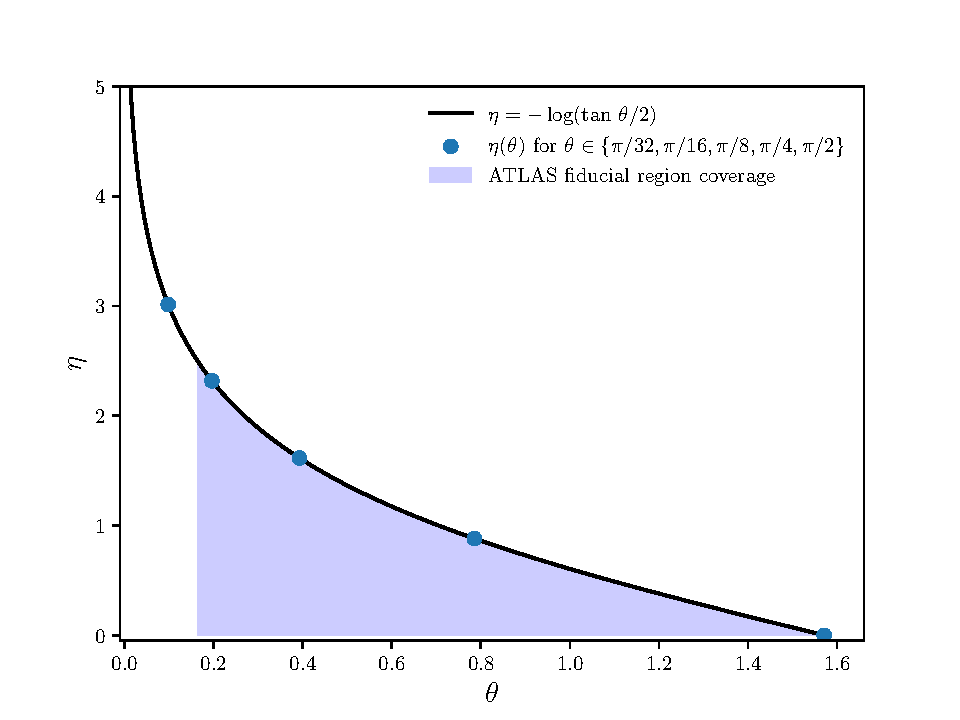
\includegraphics[width=0.8\linewidth]{preface/pseudorapidity.pdf}
 \caption[Pseudorapidity as a function of the polar angle.]{%
  Pseudorapidity, $\eta = - \ln \left(\tan \frac{\theta}{2}\right)$, as a function of the polar angle, $\theta$.
  The example markers are the points given in \Cref{table:pseudorapidity_angles}.
  The blue shaded region indicates the polar angle coverage up to $\eta = 2.5$, which is the end of the fiducial region coverage by the ATLAS inner detector.}
 \label{fig:pseudorapidity_angles}
\end{figure}

\section{Statistics}\label{section:statistics}

Statistics in particle physics

\subsection{Intervals and limits}\label{section:intervals_and_limits}

In addition to point estimates that determine an estimator, $\hat{\theta}$, of a parameter $\theta$, interval estimates give statistical precision to the measured value.
A common example of such an interval estimate is the set of points bounded by the point estimate and the estimated standard deviation: $\left[\hat{\theta} - \sigma_{\hat{\theta}}, \hat{\theta} + \sigma_{\hat{\theta}}\right]$.
The following is a short discussion of the construction, interpretation, and use of these intervals in the frequentist and Bayesian paradigms.

\subsubsection{Frequentist Confidence Intervals}

In the frequentist paradigm, a $1-\alpha$ confidence level (CL) confidence interval (CI) is an interval estimate that covers the true value of the parameter, $\theta$, $1-\alpha$ of the time it is constructed.
So the $95\%$ confidence level confidence interval covers the true value $95\%$ of the time it is constructed.
The method for constructing confidence intervals is called the ``Neyman Construction''~\cite{Neyman:1937uhy}, and results from inverting hypothesis tests.
This confidence interval construction can be described as a random variable that is the set of parameter points, $\left\{\vec{\theta}\right\}$, where the null hypothesis of each parameter point $\theta$ is accepted, $p\left(t > k_{\alpha}\middle| \theta\right) < \alpha$,

\begin{equation}
 \mathrm{CI}_{1-\alpha} = \left\{\vec{\theta}\,\middle| \,p\left(t > k_{\alpha}\middle| \vec{\theta}\right) < \alpha\right\}\,.
 \label{eq:confidence_interval}
\end{equation}

By construction, a hypothesis test of size $\alpha$ should accept the null hypothesis, given that the null is true, $(1-\alpha)$ of the time~\cite{Cranmer:2015nia}.\\

It is very important to take care in interpreting the meaning of the confidence interval, as it is often misunderstood and misused in analysis.
The confidence interval is constructed from the observed data%
\footnote{The data are a random variable in the frequentist paradigm.}
and so is a random variable and reflects information regarding the constructed estimator --- not the true parameter.
The confidence interval does \emph{not} give the interval in which there is a $1-\alpha$ probability of finding the true parameter value.
This is manifestly Bayesian and in fact is the interpretation of a Bayesian credible interval.
Keeping the definition of frequentist probability tightly in mind, the confidence interval should be interpreted as an interval of parameter values that $1-\alpha$ \emph{of the times is is constructed} contains the true parameter value.
Given this, in the frequentist paradigm one is \emph{unable} to make any statement on the probability that the true parameter value is contained in any specific confidence interval beyond the tautology that the true parameter is either contained in the it or it is not.
Any misuse of this result is not from a failing of the paradigm, but a misplaced desire of the analyst to have different questions answered than were asked.\\

In terms of computing a confidence interval, from observations that are governed by $\theta$ a test statistic, $t$, that is an estimator of $\theta$ is constructed.
For each value of the parameter to be tested, there exists an interval $\left[t_{1}, t_{2}\right]$ such that the probability of $t \in \left[t_{1}, t_{2}\right]$ is
\begin{equation}
 p\left(t_{1} < t < t_{2}\middle|\theta\right) = \int\limits_{t_{1}}^{t_{2}} f\left(t\middle|\,\theta\right)\,dt = 1-\alpha\,.
 \label{eq:confidence_interval_coverage}
\end{equation}
This interval represents a constant line segment in the $\left(t, \theta\right)$ parameter space plane at the given value of $\theta$.
By repeating this procedure for every value of $\theta$ to be tested, a band of line segments --- a ``confidence belt'' --- is created that is bound between the curves $\theta\left(t_{1}\right)$ and $\theta\left(t_{2}\right)$, as shown in the example in \Cref{fig:confidence_belt}.
Then, for any given observed value of the test statistic, $t'$, a boundary at $t = t'$ can be drawn in the plane that intersects the confidence belt at the points $\left(t', \theta_{2}\right)$ and $\left(t', \theta_{1}\right)$.
This resulting range of parameter values $\left[\theta_{1}, \theta_{2}\right]$ is the confidence interval~\cite{Cranmer:2015nia,PDG2018:Ch39}.\\

\begin{figure}[htbp]
 \centering
 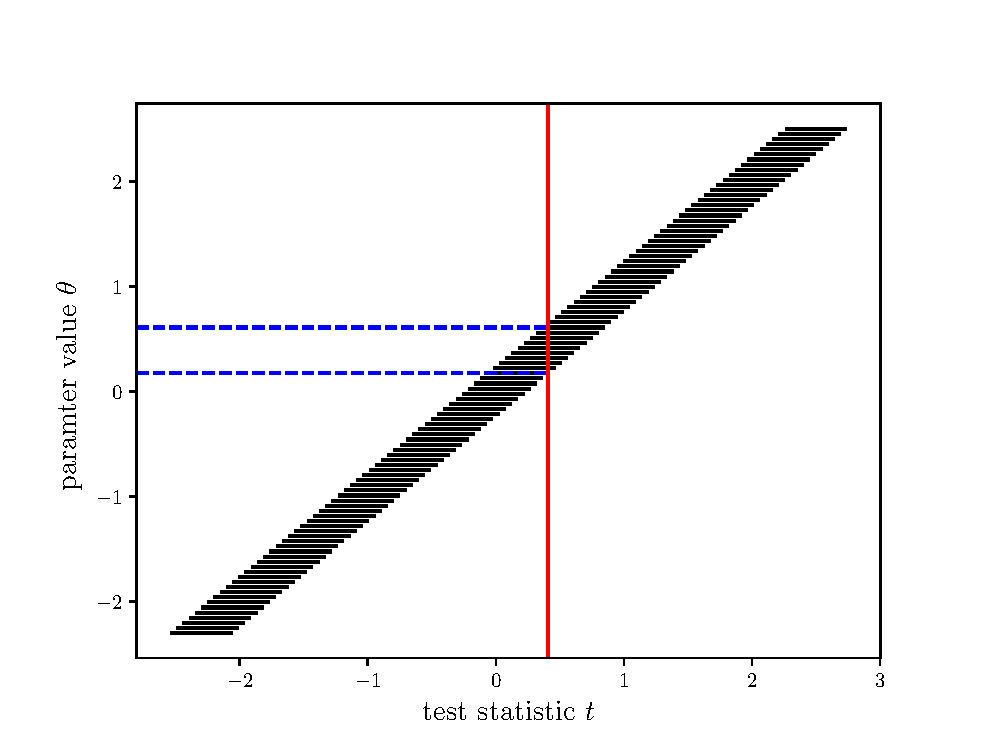
\includegraphics[width=0.4\linewidth]{preface/confidence_belt.eps}
 \caption{Example sketch of the construction of a confidence belt showing an observation in red intersecting the belt and the corresponding confidence interval as the parameter values bounded between the two blue dashed lines.}\label{fig:confidence_belt}
\end{figure}

The conditions of coverage from \Cref{eq:confidence_interval_coverage} do not uniquely specify $t_{1}$ and $t_{2}$, which allows for analysis specific choices to be made.
If central intervals are chosen, then the probabilities excluded below $t_{1}$ and $t_{2}$ are both $\alpha/2$.
In the event that only an upper (or lower) limit is of interest, as is common in searches for new physics where no excess has been observed, then the probability excluded below $t_{1}$ (or above $t_{2}$) is zero.
Alternatively, if the test statistic used is based on the likelihood ratio
\[
 \lambda = \frac{L\left(\theta\middle|\, t\right)}{L(\hat{\theta}|\, t)},
\]
the test statistic can be profiled to determine the range $\left[t_{1}, t_{2}\right]$.
Using such a test statistic results in the Feldman-Cousins confidence intervals~\cite{Feldman:1997qc}.\\

As the confidence interval can be a difficult concept to describe, a simple illustrative example follows.
Consider $n$ observations $\vec{x} = \left\{x_{1}, \cdots, x_{n}\right\}$ that are drawn from a Normal distribution with unknown mean $\theta$ and width $\sigma_{\theta}$.
This results in a sample mean $\hat{\theta}$ and standard deviation $\sigma_{\hat{\theta}}$.
To construct a $95\%$ confidence level central confidence interval for $\theta$, the test statistic $t = \left(\hat{\theta} - \theta\right)/\sigma_{\hat{\theta}}$ can be used such that ${p\left(t_{1} < t < t_{2}\middle|\theta\right) = 0.95}$, where $t_{1}$ and $t_{2}$ are respectively the $2.5$th percentile and $97.5$th percentile%
\footnote{$t_{1} = \mathrm{CDF}^{-1}\left(\alpha/2\right)$ and $t_{2} = \mathrm{CDF}^{-1}\left(1 - \alpha/2\right)$.}
of the Student's $t$-distribution for $n-1$ degrees of freedom, mean $\mu=\hat{\theta}$ and standard deviation $\sigma=\sigma_{\hat{\theta}}$.
Transforming the Student's $t$-distribution by $t' = \left(t-\hat{\theta}\right)/\sigma_{\hat{\theta}}$ to have $\mu=0, \sigma=1$ simplifies to ${p\left(-d < t' < d\middle|\theta\right) = 0.95}$.
Transforming to parameter space, ${p\left(\hat{\theta} - d\, \sigma_{\hat{\theta}} < \theta < \hat{\theta} + d\, \sigma_{\hat{\theta}}\right)  = 0.95}$, this gives a confidence interval of $\left[\hat{\theta} - d\, \sigma_{\hat{\theta}}, \hat{\theta} + d\, \sigma_{\hat{\theta}}\right]$.
Confidence intervals following this example construction are simulated and shown in \Cref{fig:confidence_intervals}.

\begin{figure}[htbp]
 \centering
 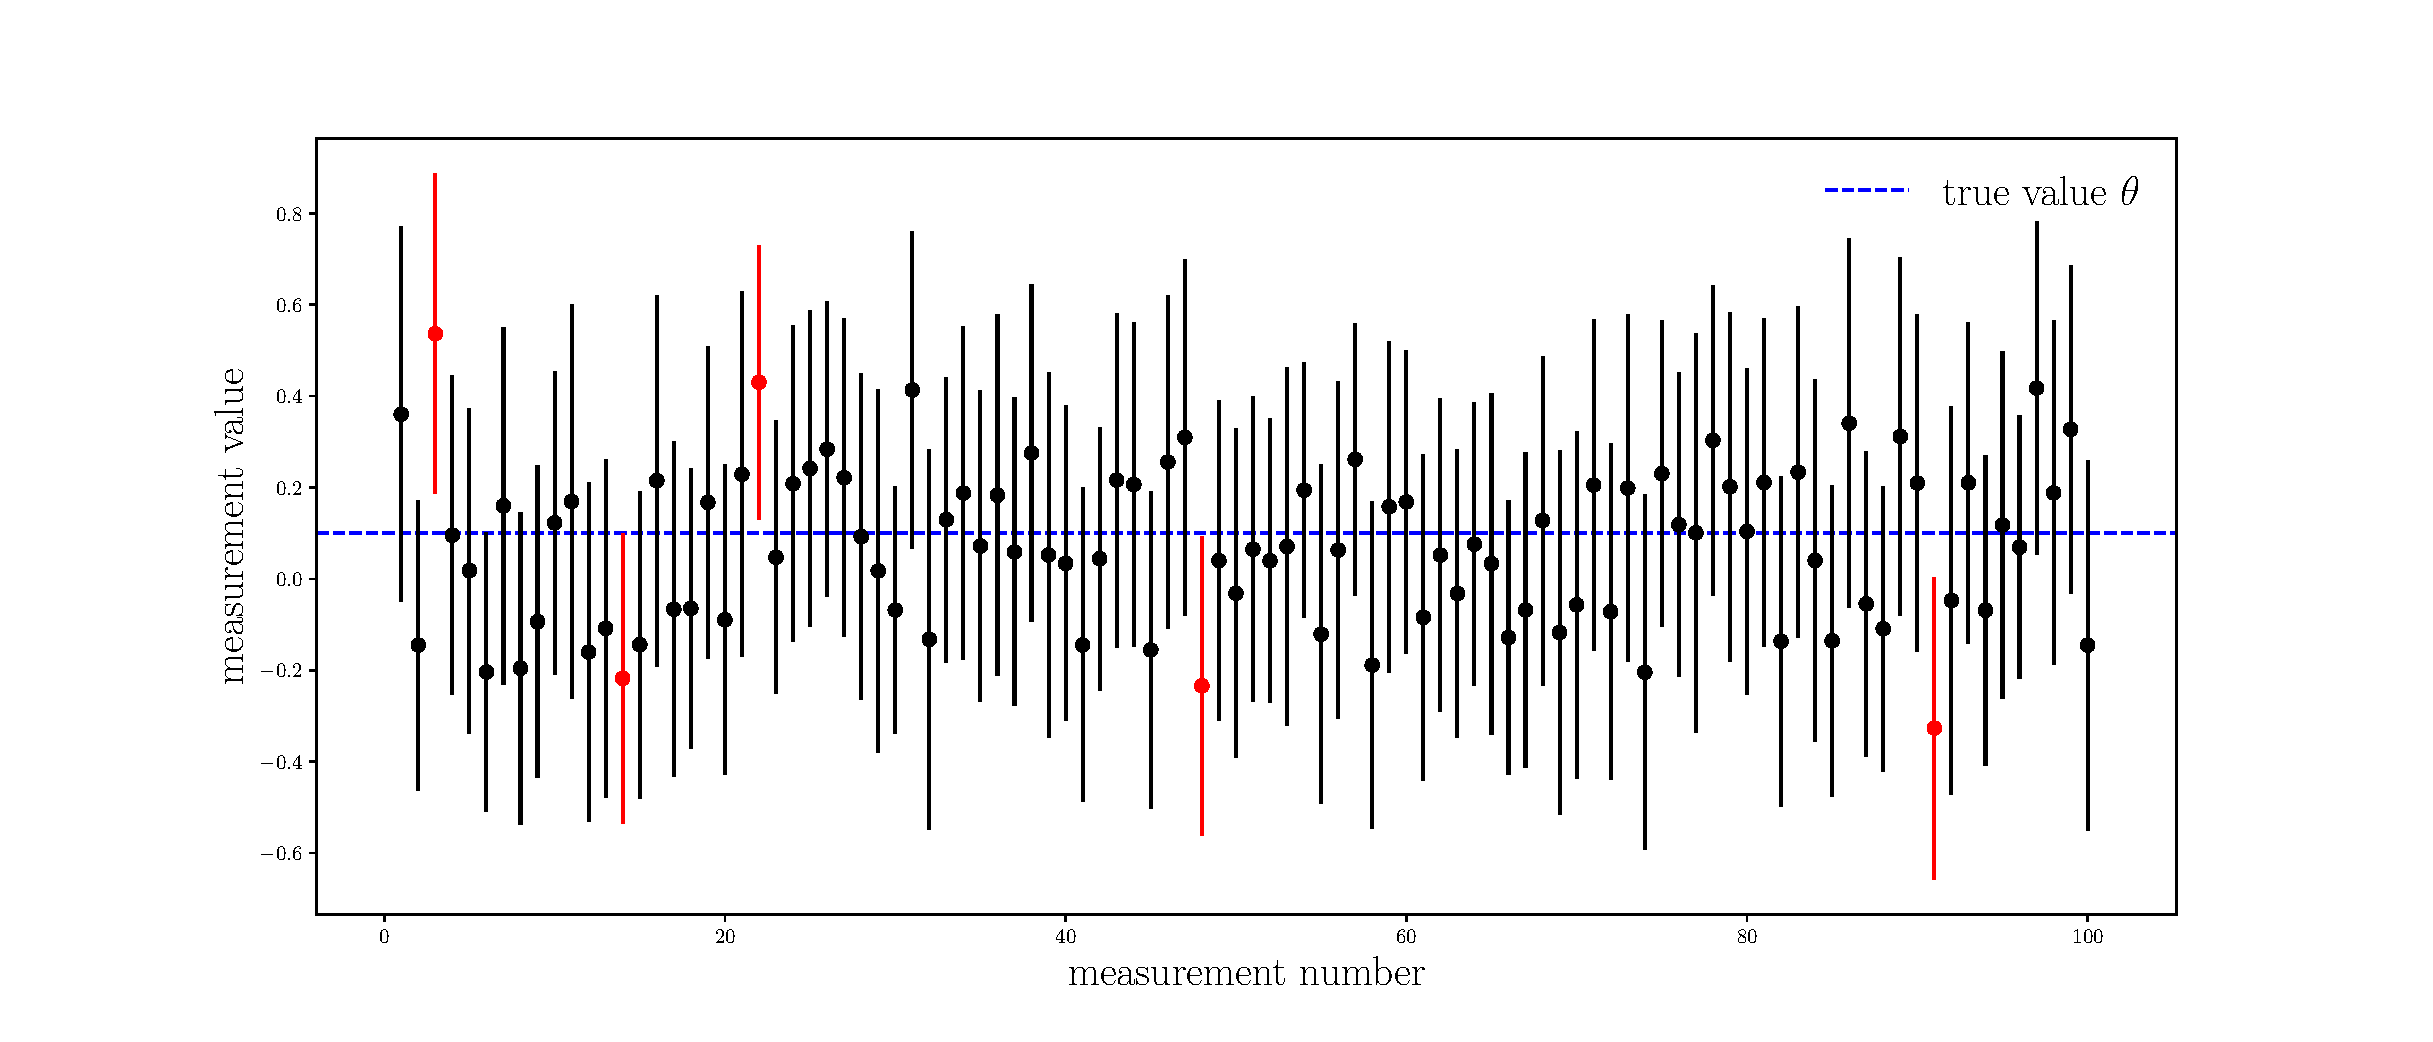
\includegraphics[width=\linewidth]{preface/confidence_intervals.eps}
 \caption{An example of 100 point estimates and associated $95\%$ confidence level confidence intervals of parameter value $\theta$.
  Confidence intervals that do not include the true value $\theta$ (dashed blue line) are colored red.}
 \label{fig:confidence_intervals}
\end{figure}

\subsubsection{Bayesian Credible Intervals}

In the Bayesian paradigm, a $1-\alpha$ credibility level (CL) credible interval (CI)%
\footnote{CL and CI are used for abbreviations for both the frequentist and Bayesian intervals.
 It will be made clear to the reader from context which paradigm is being considered.}
is an interval estimate where there is a $1-\alpha$ probability of containing the true parameter value --- which is a random variable.
As a result, it is simply the interval of the posterior predictive distribution $\left[\theta_{1}, \theta_{2}\right]$ that when integrated over gives a probability of $1-\alpha$,

\begin{equation}
 p\left(\theta_{1} < \theta < \theta_{2}\middle|\vec{x}\right) = \int\limits_{\theta_{1}}^{\theta_{2}} p\left(\theta\middle|\,\vec{x}\right)\,d\theta = 1-\alpha\,.
 \label{eq:credible_interval_coverage}
\end{equation}

As in the frequentist paradigm, there are different ways to select the credible interval range.
One can choose the shortest interval,%
\footnote{For a unimodal distribution this interval is known as the highest posterior density interval (HPD).}
the interval where probabilities excluded below $\theta_{1}$ and above $\theta_{2}$ are both $\alpha/2$ (this interval includes the median), the interval centered at the mean of the posterior (if the mean exists), or the intervals corresponding to upper (or lower) limits which reduce \Cref{eq:credible_interval_coverage} to the CDF (or CCDF) of $\theta$.\\

As a final word on interval estimates, it is worth remembering that the frequentist and Bayesian paradigms address different questions and so make different statements with their intervals.
\begin{itemize}
 \item Frequentist: When a confidence interval is constructed on future data, the constructed interval will contain the true parameter value with a probability (frequency) of $1-\alpha$.
 \item Bayesian: Given the observed data, there is a $1-\alpha$ probability that the true parameter value is contained by the constructed credible interval.
\end{itemize}


\section{Open Source Tools}\label{section:open_source}

This thesis and the researched described in it were made possible only through use of open source software.
The analysis was written in the open source languages \texttt{C++} and \texttt{Python} and made extensive use of the \texttt{ROOT} data analysis framework.
Similarly, parts of the analysis were conducted in Python and leveraged the SciPy ecosystem, most notably the NumPy and matplotlib libraries.
Additionally, the Keras library was used to interface with the TensorFlow machine learning framework for parts of the analysis.
The thesis itself was written in \LaTeXe, built using \texttt{latexmk} and \texttt{Make}, and versioned with Git.
Scientific research is built upon the open source community and tools, and this work would not have been made possible without it.


 \chapter{Introduction}\label{chapter:introduction}

The discovery of a Higgs-like boson~\cite{Higgs:1964ia,Higgs:1964pj,Higgs:1966ev,Englert:1964et,Guralnik:1964eu} at CERN in 2012 by the \Gls{ATLAS} and CMS collaborations~\cite{Aad:2012tfa,Chatrchyan:2012xdj} was a major triumph for both theoretical and experimental particle physics.
However, the properties of the new particle remain to be fully verified and the agreement of the predictions of the physics of the Higgs field by the \Gls{Standard Model} (SM) with observations of Nature require further testing.
One important property is the coupling strength of the the Higgs boson to bottom quarks $\left(\Hbb\,\right)$ --- this interaction was only experimentally observed in 2018 through associated production with a vector boson~\cite{Aaboud:2018zhk,CMS:2018abb}.
Additionally, there exist models of particle dark matter~\cite{Abdallah:2015ter} which include massive mediators between dark matter and Standard Model particles.
Such \gls{dark matter mediator}s (DMM) with couplings to Standard Model quarks would have the same decay signature to pairs of bottom quarks as the Higgs.
This thesis presents a search for low mass resonances, including Higgs, in the mass range of $100~\GeV$ to $200~\GeV$ with high momentum decaying to pairs of high momentum $b$-quarks with an associated jet $\left(\jXbb\,\right)$.
The goals of the search are to make a direct measurement of the couplings of Higgs to bottom quarks, and to search for evidence of exotic resonances with couplings to Standard Model quarks.
The thesis proceeds in the following manner.\\

\Cref{chapter:theory} introduces the field theories of the Standard Model, describes the physics of the Higgs field, and motivates the search for couplings of the Higgs to $b$-quarks and the search for exotic low mass resonances.
\Cref{chapter:LHC} introduces CERN's Large Hadron Collider and \Cref{chapter:ATLAS} describes the ATLAS experiment.
\Cref{chapter:bjet_trigger} describes the use of $b$-jet triggers in ATLAS for rapid identification of physics events with $b$-hadrons in the final state.
\Cref{chapter:event_reconstruction} gives an overview of the techniques used by the ATLAS collaboration to reconstruct the signature of particles in the ATLAS detector for physics quality data.
\Cref{chapter:analysis} is devoted to the application of the previous chapters in a search for boosted low mass resonances with a $b\bar{b}$ final state.
The results of this analysis are presented in \Cref{chapter:results}.
\Cref{chapter:software} gives a high level overview of general use statistical analysis software that was developed during the course of the analysis.
Finally, \Cref{chapter:conclusions} provides a summary of the state of measurements of Higgs couplings to heavy flavor quarks and the search for low mass exotic resonances given the results of the search, as well as an outlook to physics in Run 3 of the LHC.


 \chapter{The Standard Model and Extensions}\label{chapter:theory}

\section{The Standard Model}\label{section:standard_model}

The Standard Model of particle physics is the collection of \glspl{QFT} that describes the interactions of elementary matter with three of the four%
\footnote{Gravity is noticeably absent, as at the time of writing there is no working quantum theory of gravitation.}
known forces of Nature: the electromagnetic force, the weak nuclear force, and the strong nuclear force.
These theories collectively form a symmetry group%
\footnote{$\mathrm{SU}(n)$ is the special unitary group of degree $n$ which is the Lie group  of $n\times n$ unitary matrices with determinant of $1$.
 As the group is non-Abelian the gauge symmetries that belong to these groups are known as ``non-Abelian gauge symmetires.''}
of $\mathrm{SU}(3)_{C} \otimes \mathrm{SU}(2)_{L} \otimes \mathrm{U}(1)_{Y}$ that elegantly encode all of these interactions in a Lagrangian formalism compactly enough that they can be fully written on a single blackboard (or even further condensed down to fit on the side of a coffee mug) while giving predictions of Nature that agree fantastically with experiment for processes across 15 orders of magnitude in cross section, as seen in \Cref{fig:cross_section_experiment_theory}.
Though known to be an incomplete model, it has proven to be a successful guide and predictive tool for more than half a century.

\begin{figure}
 \centering
 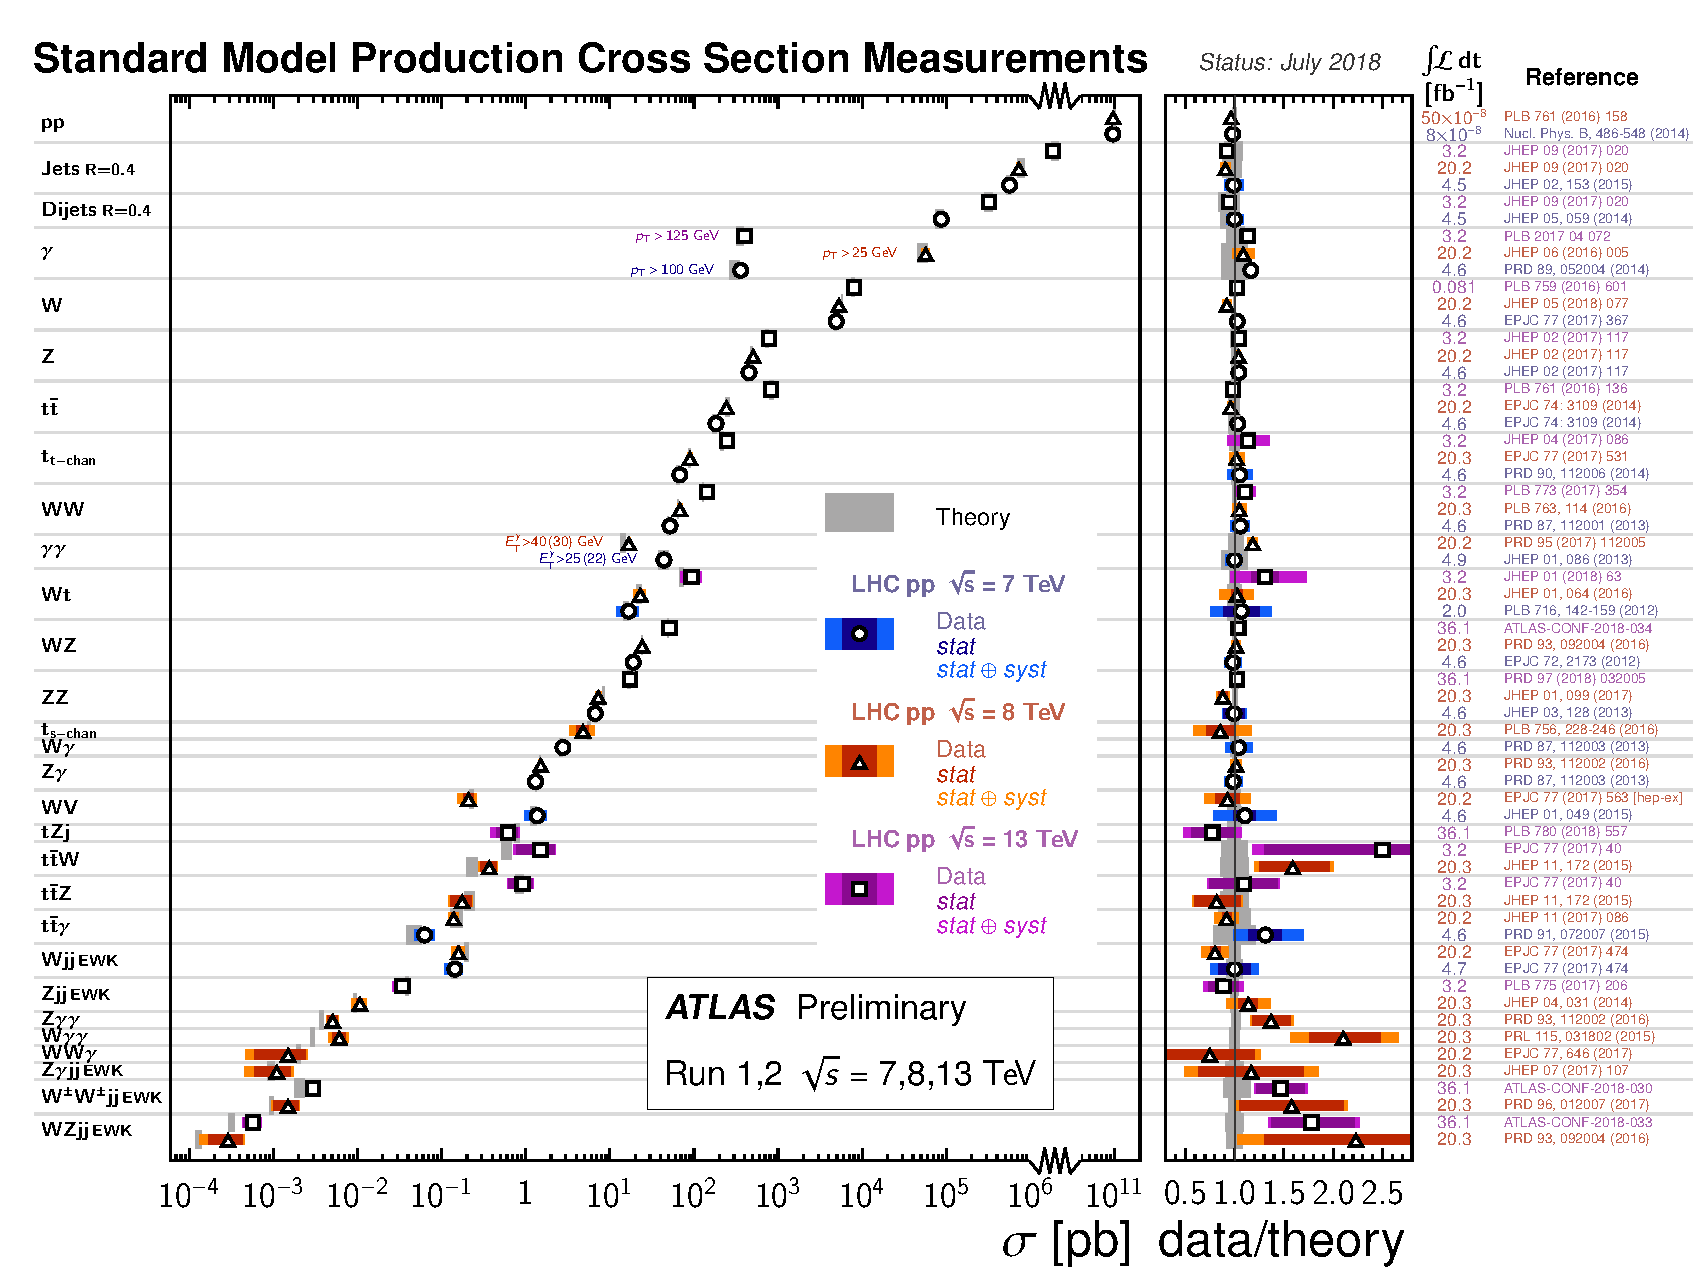
\includegraphics[width=\textwidth]{theory/ATLAS_SMSummary_FiducialXsect_rotated.eps}
 \caption[Summary of several Standard Model total and fiducial production cross section measurements using LHC proton-proton collisions, corrected for leptonic branching fractions, compared to the corresponding theoretical expectations.]{%
  Summary of several Standard Model total and fiducial production cross section measurements using LHC proton-proton collisions, corrected for leptonic branching fractions, compared to the corresponding theoretical expectations.
  All theoretical expectations were calculated at NLO or higher.
  The dark-color uncertainty bar represents the statistical uncertainty.
  The lighter-color uncertainty bar represents the full uncertainty, including systematics and luminosity uncertainties.
  The data/theory ratio, luminosity used and reference for each measurement are also shown.
  Uncertainties for the theoretical predictions are quoted from the original ATLAS papers.
  They were not always evaluated using the same prescriptions for PDFs and scales.
  The $W\gamma$ and $Z\gamma$ theoretical cross-sections have non-perturbative corrections applied to the NNLO fixed order calculations~\cite{STDM-2011-17}.
  Not all measurements are yet statistically significant~\cite{web:ATLAS_SM_summary_plots}.}
 \label{fig:cross_section_experiment_theory}
\end{figure}

The quanta of the quantum fields of the Standard Model are the particles of matter and the mediators of the fundamental forces of Nature, shown in \Cref{fig:Standard_Model}.
The spin-$1/2$ fermion fields result in the three ``generations'' of the six quarks and six leptons, which compose all matter in the Universe.
The leptons are divided into the electrically charged leptons --- the electron $(e)$, muon $(\mu)$, and tau $(\tau)$ --- and their electrically neutral neutrino counterparts --- ``flavor'' eigenstates of $\nu_{e}$, $\nu_{\mu}$, and $\nu_{\tau}$.
The quarks have fractional electric charge, with the up $(u)$, charm $(c)$, and top $(t)$ quarks having $+2/3$ elementary charge, and the down $(d)$, strange $(s)$, and bottom $(b)$ quarks having $-1/3$, as well as all of them carrying a ``color'' charge that allows them to participate in strong nuclear interactions.
They do not exist as free particles by themselves, but always in bound configurations of either two or three quarks, respectively known as ``mesons'' and ``baryons'' (e.g., pions and protons, respectively).
In addition to the matter particles are the five vector gauge bosons that are mediators of fundamental forces of Nature.
The photon $(\gamma)$ is the mediator of the electromagnetic force and interacts with all particles that carry electrical charge (i.e. the quarks, charged leptons, and charged vector bosons).
The weak nuclear force that governs nuclear interactions, such as beta decay, is mediated by the $W^{+}$, $W^{-}$, and $Z$ massive weak vector bosons.
The electrically charged $W$ bosons mediate charged flavor changing interactions between the quarks and the leptons (e.g., $c \to d + W^{+}$ and $e^{-} \to \bar{\nu}_{e} + W^{-}$), and the $Z$ boson mediates electrically neutral flavor changing interactions (e.g., $e^{+}e^{-} \to Z \to \mu^{+}\mu^{-}$ and charged lepton scattering from neutrinos).
The eight%
\footnote{As a result of the $\mathrm{SU}(3)$ symmetry.}
massless gluons mediate the strong nuclear force and so have couplings with all particles that have color charge: the quarks and the gluons themselves.
The coupling strength of the gluons varies with distance between color charged particles --- being extremely strong at close ranges and then sharply dropping of at the distance of confinement (approximately the radius of the proton).
Finally, the Higgs boson imparts mass to particles that it couples to, with stronger coupling strengths manifesting as larger masses.
This process --- which has been come to be known as the ``Higgs mechanism'' --- gives rise to the non-zero mass of the $W^{\pm}$ and $Z$ through a processes called ``electroweak symmetry breaking'' and will be discussed more throughly in \Cref{section:EWSB}.

\begin{figure}
 \centering
 \includegraphics[width=\textwidth]{theory/Standard_Model.pdf}
 \caption[Diagram of the particles of the Standard Model.]{%
  Diagram of the particles of the Standard Model.
  Shown are the three generations of fermions (the quarks and leptons), the gauge vector bosons (gluons, photon, $W^{\pm}$, and $Z$), and the Higgs boson.
  This figure was inspired and adapted from~\cite{web:Carsten_Burgard}.}
 \label{fig:Standard_Model}
\end{figure}

The following discussion of the theories that compose the Standard Model is my summary of many post-lecture conversations with former SMU professor Kent Hornbostel and readings of~\cite{Pich:2005mk}.

\clearpage
\section{Quantum Field Theories}\label{section:QFT}

\acrlong{QFT} is the mathematical framework for modern particle physics calculations.
QFT naturally incorporates quantum theory with special relativity to give a relativistic description of the interaction of quantum fields through their quantized excitations (particles).
All possible physical interactions of these fields are encoded in the terms of the Lagrangian density, $\Lagrangian$, which is a scalar and so (crucially) Lorentz invariant --- physics fundamentally works the same regardless of reference frame.
Given the ubiquity of the use of the Lagrangian density in calculations it will be interchangeably referred to as the ``Lagrangian'' henceforth, with hopefully minimal confusion.
Additionally, the Lagrangian density must be locally gauge invariant; meaning that it is invariant under certain Lie group transformations.
Local gauge invariance is an expression that representations of the Lagrangian density that result in the same physical interactions must be equivalently valid.
A local gauge symmetry is distinct from a global gauge symmetry, as would arise in Noether's theorem, in that a local gauge symmetry results in a gauge invariance for the spacetime point of consideration, but is not guaranteed to be valid in all cases.
That is, a global gauge symmetry is in some sense a special case of a local gauge symmetry, where the symmetry applies for all points.
As an example, consider the Dirac Lagrangian
\begin{equation}
 \Lagrangian_{\textrm{Dirac}} = \bar{\psi} \left(i \gamma^{\mu}\partial_{\mu} - m\right)\psi.
 \label{eq:Dirac_Lagrangian}
\end{equation}
If a global gauge transformation of a phase shift is applied,
\[
 \psi \to e^{-i\theta} \psi, \qquad \bar{\psi} \to \bar{\psi}\,e^{i\theta},
\]
then it is readily seen that the Lagrangian has remained invariant
\[
 \Lagrangian \to \bar{\psi} \left(i \gamma^{\mu}\partial_{\mu} - m\right)\psi.
\]
However, if a local gauge transformation of a phase shift dependent on the field's spacetime is applied
\[
 \psi \to e^{-i\theta(x)} \psi, \qquad \bar{\psi} \to \bar{\psi}\,e^{i\theta(x)},
\]
then for the Lagrangian
\[
 \Lagrangian \to \bar{\psi} \left(i \gamma^{\mu}\partial_{\mu} - m\right)\psi + \bar{\psi}\, \gamma^{\mu} \left(\partial_{\mu} \theta\right)\psi
\]
to preserve the definition of the four-gradient under such a local transformation requires the addition of a gauge field $A_{\mu}(x)$ to form the covariant%
\footnote{``Covariant'' in that it transforms with the gauge fields so that the derivative remains unchanged.}
derivative,
\[
 D_{\mu} \equiv \partial_{\mu} - iq A_{\mu}(x),
\]
with local gauge transformation
\[
 A_{\mu} \to A_{\mu} - \frac{1}{q} \partial_{\mu}\theta,
\]
such that
\[
 \theta(x) = q \Lambda(x),
\]
resulting in the nice covariant form
\[
 \Lagrangian \to \bar{\psi} \left(i \gamma^{\mu}D_{\mu} - m\right)\psi = \bar{\psi} \left(i \slashed{D} - m\right)\psi.
\]
Given the implications of local gauge invariance, the gauge may be arbitrarily chosen to simplify calculations with no less of generality.

Two examples of highly successful \glspl{QFT} are \gls{QED} and \gls{QCD}, which are briefly discussed here.

\subsection{Quantum Electrodynamics (QED)}\label{subsection:QED}

The Glashow-Weinberg-Salam theory of electromagnetic interactions~\cite{Glashow:1961tr,Goldstone:1962es,Weinberg:1967tq} defines electromagnetic interactions of matter in the Standard Model.
The Lagrangian density for QED --- which describes the interactions of a spin-$1/2$ field with the electromagnetic field --- possesses a global $\mathrm{U}(1)$ symmetry, manifest through the conservation of electric charge, and is given by
\begin{equation}
 \Lagrangian_{\textrm{QED}} = -\frac{1}{4}F_{\mu\nu} F^{\mu\nu} + \bar{\psi} \left(i \slashed{D} - m\right)\psi
 \label{eq:QED_Lagrangian}
\end{equation}
where $F_{\mu\nu} = \partial_{\mu}A_{\nu} - \partial_{\nu}A_{\mu}$ is the electromagnetic field strength tensor.
In the QED Lagrangian, the kinetic term $-\frac{1}{4}F_{\mu\nu} F^{\mu\nu}$ describes the behavior of the electromagnetic field --- which along with the Euler-Lagrange equations result in Maxwell's equations --- and the term $\bar{\psi} \left(i \slashed{D} - m\right)\psi$ gives the interactions of the electromagnetic field with charged particles.

\subsection{Quantum Chromodynamics (QCD)}\label{subsection:QCD}

\gls{QCD} is the gauge field theory that describes the interactions of quarks and gluons governed by the strong nuclear force, and characterized by a $\mathrm{SU}(3)$ symmetry.
The QCD Lagrangian density is
\begin{equation}
 \Lagrangian_{\textrm{QCD}} = -\frac{1}{4}G_{\mu \nu}^{a} G_{a}^{\mu \nu} + \sum_{f} i \bar{\psi}_{f} D_{\mu} \gamma^{\mu} \psi_{f},
 \label{eq:QCD_Lagrangian}
\end{equation}
for the $f$ families of quarks, $\psi_{f}$.
The Lagrangian is written without the color index for readability, but, as both the quarks and gluons carry a color charge, then the quark fields $\psi$ are column vectors with color index $\alpha$ and the gluon fields $G_{\mu}^{a}$ are matrices with color indices $\alpha$ and $\beta$.
The kinetic term $-\frac{1}{4}G_{\mu \nu}^{a} G_{a}^{\mu \nu}$ describes the self interactions of the gluon fields $G_{\mu}^{a}$ given the gluon field strength tensor $G_{\mu\nu}^{a} = \partial_{\mu} G_{\nu}^{a} - g_{s} f^{abc} G_{\mu}^{b} G_{\nu}^{c}$
for strong coupling constant $g_{s}$ and $\mathrm{SU}(3)$ structure constants $f^{abc}$.
The term $\sum_{f} i \bar{\psi}_{f} D_{\mu} \gamma^{\mu} \psi_{f}$ with covariant derivative
\[
 D_{\mu} = \partial_{\mu} - i g_{s} G_{\mu}^{a} T^{a},
\]
where $T^{a}$ are the generators of the $\mathrm{SU}(3)$ symmetry group, is the kinetic term for the quarks and describes the interactions between quarks and gluons.
All terms in the Lagrangian density that involve quarks and gluons are color singlets, which promotes the idea of ``color confinement.''
In Nature this color confinement is seen empirically by the observation of quarks only in bound states with other quarks that are colorless --- i.e., free quarks have never been directly observed.
These bound states of quarks are known as ``hadrons.''
Half-integer spin hadrons formed from an even number of quarks are known as ``mesons,'' and integer spin hadrons formed from an odd number of quarks are known as ``baryons.''
In strong interactions at hadron colliders there is enough energy to break individual quarks and gluons out of their hadronic forms, however these free partons then immediately ``hadronize'' by forming bound states with other quarks, even if that requires sacrificing some of their energy to pull another quark from the vacuum.
This process of hadronization, and subsequent decays, creates a shower of hadrons and leptons that is collectively referred to as a ``jet'' and will be discussed more in \Cref{section:jets}.
Jets play an important role in understanding the physics of QCD, and the observation of three jet systems is the best experimental evidence of the existence of gluons~\cite{Brandelik:1979bd,Ellis:1978wp,Andersson:1983ia,Brandelik:1980vs}.

QCD is a deeply rich theory that deserves much attention (c.f.~\cite{Campbell:2017hsr}), but for the purposes of this thesis it will only be introduced here to motivate a more complete picture of the QFTs that build the Standard Model.

\section{Spontaneous Symmetry Breaking}\label{section:symmetry_breaking}

Spontaneous symmetry breaking is the process by which a physical system that has a symmetry does not express that symmetry for perturbations around the ground state of the system.
It is worth noting, given the somewhat confusing nature of the use of ``breaking,'' that the symmetry of the Lagrangian is not destroyed under symmetry breaking, but rather is not manifest given the ground state into which the system has been perturbed.
A classical example of spontaneous symmetry breaking is that of a pen being balanced upright on its tip on a table.
In the unstable equilibrium state of the pen being balanced (the high energy/excited state configuration) the pen possesses a $\mathrm{U}(1)$ symmetry of rotation about its axis.
If the pen is perturbed from this state by a small vibration it will fall into its ground state onto the surface of the table and will lie along some direction ``breaking'' the symmetry that was exhibited by the previous state.
Another example is that of Heisenberg’s model of the ferromagnet, which has Hamiltonian of $\mathcal{H} = -\sum_{i\neq j} J_{ij}\,\vec{s}_{i} \cdot \vec{s}_{j}$ across neighboring atoms.
This Hamiltonian also possesses as rotational symmetry above the Curie temperature --- rotating all the spins by some amount leaves the total spin of the system invariant.
However, below the Curie temperature a non-zero magnetization will arise along a particular direction which will cause all spins to become aligned parallel to it, breaking the symmetry.

A final illustrative toy model, that will prove useful in the context of the Higgs mechanism, is that of a massive complex scalar field
\[
 \phi = \frac{1}{\sqrt{2}} \left(\phi_{1} + i \phi_{2}\right),
\]
with Lagrangian density
\[
 \Lagrangian = \partial_{\mu}\phi^{\dagger}\partial^{\mu}\phi + m^{2}\phi^{\dagger}\phi - \frac{\lambda}{4} \left(\phi^{\dagger}\phi\right)^{2}
\]
composed of the kinetic term, $\partial_{\mu}\phi^{\dagger}\partial^{\mu}\phi$, and the potential $V\left(\phi\right) = -m^{2}\phi^{\dagger}\phi + \frac{\lambda}{4} \left(\phi^{\dagger}\phi\right)^{2}$.
The potential is zero at $\phi=0$, but has its minima occur at
\[
 \phi^{\dagger}\phi = \frac{1}{2}\left(\phi_{1}^{2} - \phi_{2}^{2}\right) = \frac{2m^2}{\lambda} \equiv \frac{1}{2}v^{2}
\]
with magnitude
\[
 \abs{\phi} = \frac{1}{\sqrt{2}}v = \frac{\sqrt{2} v}{\lambda^{1/2}}.
\]
It is seen that this potential possesses a $\mathrm{U}(1)$ symmetry, such that it is invariant under $\phi \to e^{-i\theta}\phi$, resulting in an infinite number of possible minima.
Rewriting the fields using polar coordinates in field space,
\[
 \phi(x) = \frac{1}{\sqrt{2}} \rho\left(x\right) e^{-i \theta(x)/v},
\]
and choosing the arbitrary ground state --- breaking the symmetry --- of $\rho=v$ and $\theta=0$ then allows for the redefinition of the fields as
\[
 \phi(x) = \frac{1}{\sqrt{2}} \left(v + h\left(x\right)\right) e^{-i \theta(x)/v},
\]
where $h$ and $\theta$ become the normal modes.
Perturbations about the minima result in massive radial $h$ modes and massless rotational $\theta$ modes.
These radial modes result in a massive particle, and the rotational modes result in massless particles known as Nambu-Goldstone bosons~\cite{Nambu:1960tm,Goldstone:1961eq}.

\section{Electroweak Symmetry and Interactions}\label{section:EW_interactions}

The electroweak interactions are encoded in the symmetry group $\mathrm{SU}(2)_{L} \otimes \mathrm{U}(1)_{Y}$, where $\mathrm{SU}(2)$ is the symmetry of weak-isospin and $Y$ is weak-hypercharge.
The gauge group requires all left-handed spinors to be doublets, and the right-handed spinors to be singlets.
Considering only the first generation of quarks and leptons, this can be written for the leptons as
\[
 \psi_{e\,1}\left(x\right) = \begin{pmatrix}
  \nu_{e} \\
  e^{-}
 \end{pmatrix}_{L},\quad
 \psi_{e\,2}\left(x\right) = \nu_{e\,R},\quad
 \psi_{e\,3}\left(x\right) = e_{R}^{-}\,,
\]
and for the quarks as
\[
 \psi_{u\,1}\left(x\right) = \begin{pmatrix}
  u \\
  d
 \end{pmatrix}_{L},\quad
 \psi_{u\,2}\left(x\right) = u_{R},\quad
 \psi_{u\,3}\left(x\right) = d_{R}\,.
\]
The ``free'' Lagrangian density (the kinetic term) is then
\[
 \Lagrangian = \sum_{j=1}^{3} i \,\bar{\psi}_{e\,j}\left(x\right) \slashed{\partial} \,\psi_{e\,j}\left(x\right) + i \,\bar{\psi}_{u\,j}\left(x\right) \slashed{\partial} \,\psi_{u\,j}\left(x\right)\,,
\]
which should be invariant under local gauge transformations of the symmetry group,
\[
 \begin{split}
  \psi_{e\,1}&\left(x\right) \to e^{iy_{1} \beta(x)}\, U_{L}\left(x\right)\psi_{e\,1}\left(x\right), \qquad U_{L}\left(x\right) = \exp\left(i\,\frac{\tau^{i}}{2} \alpha^{i}(x)\right)\\
  \psi_{e\,2}&\left(x\right) \to e^{iy_{2} \beta(x)}\, \psi_{e\,2}\left(x\right)\\
  \psi_{e\,3}&\left(x\right) \to e^{iy_{3} \beta(x)}\, \psi_{e\,3}\left(x\right)
 \end{split}
\]
The generators of $\mathrm{SU}(2)$ are the Pauli spin matrices,
\[
 \tau^{0} = \begin{pmatrix}%
  1 & 0 \\%
  0 & 1
 \end{pmatrix},\quad
 \tau^{1} = \begin{pmatrix}%
  0 & 1 \\%
  1 & 0
 \end{pmatrix},\quad
 \tau^{2} = \begin{pmatrix}%
  0 & -i \\%
  i & 0
 \end{pmatrix},\quad
 \tau^{3} = \begin{pmatrix}%
  1 & 0  \\%
  0 & -1 %
 \end{pmatrix}\,,%
\]
and the resulting four degrees of freedom (three from $\mathrm{SU}(2)$ and one from $\mathrm{U}(1)$) manifest as the gauge bosons of the weak vector fields $W_{\mu}^{k}\left(x\right)$:
\[
 B_{\mu}\left(x\right) = W_{\mu}^{0}\left(x\right)\tau^{0}, \qquad \vec{W}_{\mu}\left(x\right) = W_{\mu}^{i}\left(x\right)\frac{\tau^{i}}{2}\,.
\]
As a result, the covariant derivative is
\begin{align}
 D_{\mu}\psi_{1}(x) & = \left(\partial_{\mu} - ig_{1}\, y_{1} B_{\mu}(x) - ig_{2} \vec{W}_{\mu}(x)\right)\psi_{1}(x)\label{eq:EW_derivative} \\
 D_{\mu}\psi_{2}(x) & = \left(\partial_{\mu} - ig_{1}\, y_{2} B_{\mu}(x)\right)\psi_{2}(x)\notag                                             \\
 D_{\mu}\psi_{3}(x) & = \left(\partial_{\mu} - ig_{1}\, y_{3} B_{\mu}(x)\right)\psi_{3}(x)\notag
\end{align}
for weak hypercharge $y_{i}$ coupling $g_{1}$ and weak isospin coupling $g_{2}$, this gives the requirements for the local transformations of the vector gauge fields,
\[
 B_{\mu}(x) \to B_{\mu}(x) + \frac{1}{g_{1}} \partial_{\mu}\beta(x), \qquad%
 \vec{W}_{\mu}(x) \to U_{L}(x)\vec{W}_{\mu}(x)\,U_{L}^{\dagger}(x) - \frac{i}{g_{2}} \left(\partial_{\mu}U_{L}(x)\right)
 U_{L}^{\dagger}(x)
\]
The kinetic term of the electroweak vector gauge field Lagrangian density is then seen to be
\[
 \Lagrangian_{\textrm{kinetic}} = -\frac{1}{4}B_{\mu\nu}B^{\mu\nu} - \frac{1}{2}\mathrm{Tr}\left(\vec{W}_{\mu\nu}\vec{W}^{\mu\nu}\right) = -\frac{1}{4}B_{\mu\nu}B^{\mu\nu} -\frac{1}{4} W_{\mu\nu}^{i} W_{i}^{\mu\nu}.
\]
It is seen that the $\mathrm{SU}(2)_{L} \otimes \mathrm{U}(1)_{Y}$ gauge symmetry forbids a mass term for the vector fields, and fermion masses are also forbidden as the term would mix the left and right handed fields which have different transformation properties --- which would explicitly break the gauge symmetry.

\subsection{Electroweak Interactions}

Given the covariant derivative, \Cref{eq:EW_derivative}, and resulting Lagrangian density for the fermions,
\[
 \Lagrangian = \sum_{j=1}^{3} i \,\bar{\psi}_{e\,j}\left(x\right) \slashed{D} \,\psi_{e\,j}\left(x\right) + i \,\bar{\psi}_{u\,j}\left(x\right) \slashed{D} \,\psi_{u\,j}\left(x\right)\,,
\]
it is seen that there are interactions between the fermions and the vector gauge fields (dropping fermion index for compactness),
\[
 \Lagrangian \subset g_{2} \bar{\psi}_{1} \gamma^{\mu}\vec{W}_{\mu} \psi_{1} + g_{1} B_{\mu} \sum_{j=1}^{3} y_{j}\bar{\psi}_{j} \gamma^{\mu} \,\psi_{j}\,.
\]
The first term, which contains the $\mathrm{SU}(2)_{L}$ matrix
\[
 \vec{W}_{\mu} = W_{\mu}^{i}(x) \frac{\tau^{i}}{2} = \frac{1}{\sqrt{2}} \begin{pmatrix}%
  \sqrt{2} W_{\mu}^{3} & W_{\mu}^{\dagger}     \\
  W_{\mu}              & -\sqrt{2} W_{\mu}^{3}
 \end{pmatrix}\,,
\]
gives rise to the charged current interactions of the charged $W$ boson fields
\[
 W_{\mu} = \frac{1}{\sqrt{2}} \left(W_{\mu}^{1}  + i W_{\mu}^{2}\right), \qquad W_{\mu}^{\dagger} = \frac{1}{\sqrt{2}} \left(W_{\mu}^{1}  - i W_{\mu}^{2}\right)
\]
with the left-handed quarks and charged leptons, seen in \Cref{fig:EW_W_quarks} and \Cref{fig:EW_W_leptons}.
Likewise, through mixing of the neutral $W_{\mu}^{3}$ and $B_{\mu}$ fields,
\[
 \begin{pmatrix}
  A_{\mu} \\
  Z_{\mu}
 \end{pmatrix}
 = \begin{pmatrix}
  \cos\theta_{W}  & \sin\theta_{W} \\
  -\sin\theta_{W} & \cos\theta_{W}
 \end{pmatrix}
 \begin{pmatrix}
  B_{\mu} \\
  W_{\mu}^{3}
 \end{pmatrix}\,,
\]
with Weinberg mixing angle
\[
 \sin\theta_{W} = \frac{g_{1}}{\sqrt{g_{1}^{2} + g_{2}^{2}}}, \qquad \cos\theta_{W} = \frac{g_{2}}{\sqrt{g_{1}^{2} + g_{2}^{2}}},
\]
the mass eigenstates of the $Z$ boson and photon arise
\[
 \begin{split}
  Z_{\mu} &= W_{\mu}^{3} \cos\theta_{W} - B_{\mu} \sin\theta_{W} = \frac{1}{\sqrt{g_{1}^{2} + g_{2}^{2}}} \left(g_{2} W_{\mu}^{3} - g_{1} B_{\mu}\right) \\
  A_{\mu} &= W_{\mu}^3 \sin\theta_{W} + B_{\mu} \cos\theta_{W} = \frac{1}{\sqrt{g_{1}^{2} + g_{2}^{2}}} \left(g_{1} W_{\mu}^{3} + g_{2} B_{\mu}\right)
 \end{split}
\]
which mediate the neutral current interactions with the fermions, seen in \Cref{fig:EW_Z} and \Cref{fig:QED_photon}.

\begin{figure}[htbp]
 \centering
 \begin{subfigure}[t]{0.23\textwidth}
  \centering
  \includegraphics[width=\textwidth]{theory/QED_photon.pdf}
  \caption[The vertex for interactions of an electrically charged particle and a photon.]{%
   The vertex for interactions of an electrically charged particle and a photon.}
  \label{fig:QED_photon}
 \end{subfigure}%
 \quad
 \begin{subfigure}[t]{0.23\textwidth}
  \centering
  \includegraphics[width=\textwidth]{theory/electroweak_Z.pdf}
  \caption[The vertex for neutral current interactions of an fermion and a $Z$ boson.]{%
   The vertex for neutral current interactions of an fermion and a $Z$ boson.}
  \label{fig:EW_Z}
 \end{subfigure}%
 \quad
 \begin{subfigure}[t]{0.23\textwidth}
  \centering
  \includegraphics[width=\textwidth]{theory/electroweak_W_quarks.pdf}
  \caption[The vertex for charged current interactions of quarks with a $W$ boson.]{%
   The vertex for charged current interactions of quarks with a $W$ boson.}
  \label{fig:EW_W_quarks}
 \end{subfigure}%
 \quad
 \begin{subfigure}[t]{0.23\textwidth}
  \centering
  \includegraphics[width=\textwidth]{theory/electroweak_W_leptons.pdf}
  \caption[The vertex for charged current interactions of a charged lepton and neutrino with a $W$ boson.]{%
   The vertex for charged current interactions of a charged lepton and neutrino with a $W$ boson.}
  \label{fig:EW_W_leptons}
 \end{subfigure}%
 \caption[The Feynman diagrams for allowed QED and electroweak interactions.]{%
  The Feynman diagrams for allowed QED and electroweak interactions in the Standard Model.}
 \label{fig:electroweak_vertices}
\end{figure}

\section{Electroweak Symmetry Breaking}\label{section:EWSB}

To break the electroweak symmetry and provide masses to the weak vector bosons, consider the discussion given in \Cref{section:symmetry_breaking} and a complex scalar doublet (introduced by, among others~\cite{Guralnik:1964eu,Kibble:2015mwa}, Brout and Englert~\cite{Englert:1964et}, and Higgs~\cite{Higgs:1964ia,Higgs:1964pj})
\begin{equation}
 \phi = \begin{pmatrix}%
  \phi^{+} \\%
  \phi^{0}
 \end{pmatrix} = \frac{1}{\sqrt{2}} \begin{pmatrix}%
  \phi_{1} + i \phi_{2} \\%
  \phi_{3} + i \phi_{4}%
 \end{pmatrix}%
 \label{eq:Higgs_doublet}
\end{equation}
with Lagrangian density
\begin{equation}
 \Lagrangian_{\textrm{Higgs}} = \left(D_{\mu}\phi\right)^{\dagger}D^{\mu}\phi - \mu^{2}\phi^{\dagger}\phi - \lambda \left(\phi^{\dagger}\phi\right)^{2}
 \label{eq:Higgs_Lagrangian}
\end{equation}
that is invariant under local $\mathrm{SU}(2)_{L} \otimes \mathrm{U}(1)_{Y}$ transformations.
The Higgs potential
\begin{equation}
 V\left(\phi\right) = \mu^{2}\phi^{\dagger}\phi + \lambda \left(\phi^{\dagger}\phi\right)^{2},
 \label{eq:Higgs_potential}
\end{equation}
shown in \Cref{fig:Higgs_potential}, is chosen such that $\mu^{2} < 0$ and $\lambda > 0$ to provide stable minima.
As before in \Cref{section:symmetry_breaking} with the case of the toy model of the massive complex scalar field, once a ground state has been arbitrarily chosen this spontaneously breaks the $\mathrm{SU}(2)_{L} \otimes \mathrm{U}(1)_{Y}$ symmetry to the subgroup $\mathrm{U}(1)_{\textrm{QED}}$.
This time, the four fields of the complex scalar doublet are reparameterized into
\[
 \phi(x) = \frac{1}{\sqrt{2}} \begin{pmatrix}
  0 \\
  v + h(x)
 \end{pmatrix}
 \exp\left(i \frac{\tau^{i}}{2} \theta^{i}(x)\right)
\]
which gives the real scalar field $h(x)$, corresponding to radial perturbations of the minima, and three%
\footnote{There is much beauty in electroweak symmetry breaking, but the simple, insightful choice of the doublet to give as many Nambu-Goldstone bosons as vector gauge fields is marvelous.}
Nambu-Goldstone fields $\theta^{i}(x)$ with rotational symmetry --- their values have become gauge choices.
Exploiting this gauge freedom, and choosing the unitary gauge $\theta^{i}(x)=0$, results in kinetic term $\left(\textrm{where } g = \sqrt{g_{1}^{2} + g_{2}^{2}}\right)$
\[
 \Lagrangian \subset \frac{1}{2}\partial_{\mu} h \partial^{\mu} h + \left(v + h\right)^{2} \left(\frac{g^{2}}{4} W_{\mu}^{\dagger}W^{\mu} + \frac{g^{2}}{8 \cos^2 \theta_{W}} Z_{\mu}^{\dagger}Z^{\mu}\right)
\]
where the $W^{\pm}$ and $Z$ bosons have absorbed the Nambu-Goldstone bosons as polarizations and respectively acquired masses of
\[
 m_{W} = \frac{1}{2}vg, \qquad m_{Z} = \frac{m_{W}}{\cos\theta_{W}} = \frac{vg}{2\cos\theta_{W}}\,.
\]
Through self-coupling the scalar field --- the Higgs field --- also acquires a mass term of
\[
 m_{h} = \sqrt{-2\mu^{2}} = \sqrt{2\lambda}v.
\]
In the Standard Model $v$, $g_{1}$, $g_{2}$ are free parameters to be measured by experiment, and so the masses of the bosons are not directly predicted.
However, the value%
\footnote{Often referred to as the ``weak scale'' or the ``vacuum expectation value.''}
of $v$ has been calculated independently~\cite{Plehn:2005nk} to be approximately $246~\GeV$.
It is also noted that in further interactions the quarks and charged leptons acquire a mass term from Yukawa couplings~\cite{Yukawa:1935xg}, $c_i$, with the Higgs field
\[
 \begin{split}
  \Lagrangian_{\textrm{Yukawa}} &= -\frac{1}{\sqrt{2}} \left(v+h\right) \left(c_{1}\bar{d}d + c_{2}\bar{u}u + c_{3}\bar{e}e\right) \\
  &= - \left(1 + \frac{h}{v}\right)\left(m_{d}\bar{d}d + m_{u}\bar{u}u + m_{e}\bar{e}e\right)\,.
 \end{split}
\]
The neutrinos notably do not participate in this interaction, and their observed non-zero mass~\cite{Ahmad:2001an} is unexplained through electroweak symmetry breaking in the Standard Model and is currently unresolved.

\begin{figure}[htbp]
 \centering
 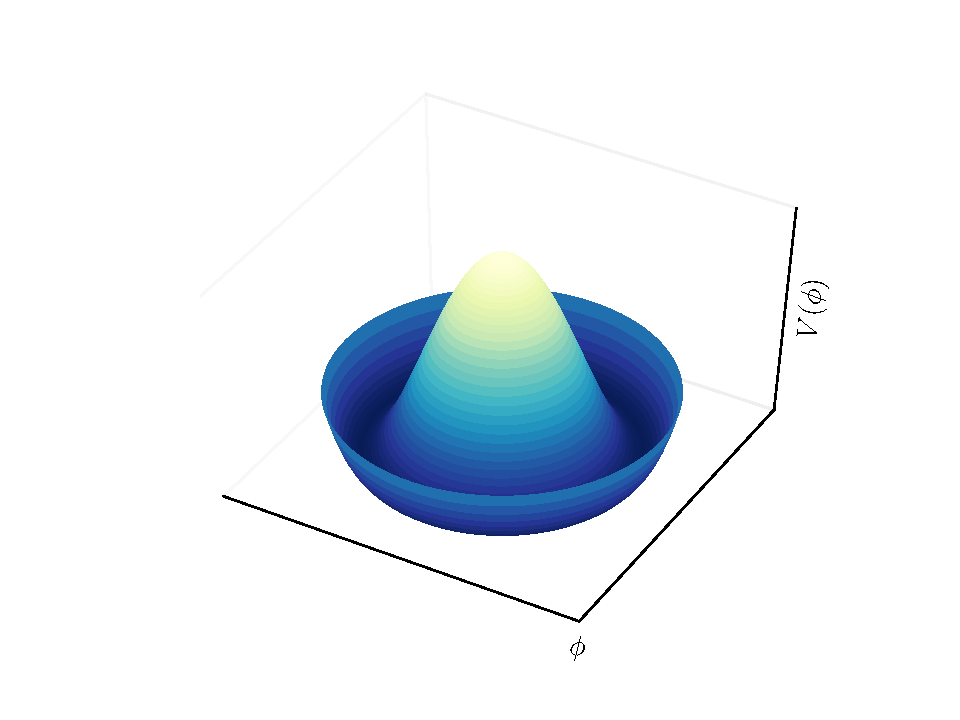
\includegraphics[width=\linewidth]{theory/higgs_potential.pdf}
 \caption[Sketch of the Higgs potential shape.]{%
 Sketch of the Higgs potential's ``wine bottle'' shape.
 The trough (the bottom of the eponymous wine bottle) are the infinite choices of minima at the vacuum expectation value, $v$, that can be selected upon spontaneously breaking the $\mathrm{SU}(2)_{L} \otimes \mathrm{U}(1)_{Y}$ symmetry to the subgroup $\mathrm{U}(1)_{\textrm{QED}}$.}
 \label{fig:Higgs_potential}
\end{figure}

\section{The Higgs Boson}\label{section:Higgs_boson}

The massive Higgs boson produced though the ``Higgs mechanism'' approach to electroweak symmetry breaking is a particle of great interest, as the interactions of the Higgs field with all other elementary particle fields generates their mass.
As a result, through these couplings the Higgs boson can be produced through a large number of interactions.
As this thesis is focused on experimental efforts at CERN's \gls{LHC}, the production mechanisms of interest will be the leading ones in a hadron collider with center-of-mass energy $\sqrt{s}=13~\TeV$.
In order of decreasing cross section, those production modes are: gluon-gluon fusion (ggF), vector boson fusion (VBF), vector boson-associated production or ``Higgsstrahlung'' (VH), and associated production with $t\bar{t}$ ($t\bar{t}H$) and $b\bar{b}$ ($b\bar{b}H$), seen in \Cref{fig:Higgs_production_diagrams}.
The predicted cross section for these production modes are given in \Cref{table:Higgs_production_cross_section} and plotted with theory uncertainties in \Cref{fig:Higgs_production_cross_section_theory}.

\begin{figure}[htbp]
 \centering
 \begin{subfigure}[t]{0.48\textwidth}
  \centering
  \includegraphics[width=\textwidth]{theory/Higgs_ggF.pdf}
  \caption[Feynman diagram for Higgs production through gluon-gluon fusion.]{%
   Feynman diagram for Higgs production through gluon-gluon fusion.}
  \label{fig:Higgs_ggF}
 \end{subfigure}%
 \quad
 \begin{subfigure}[t]{0.48\textwidth}
  \centering
  \includegraphics[width=\textwidth]{theory/Higgs_VBF.pdf}
  \caption[Feynman diagram for Higgs production through vector boson fusion.]{%
   Feynman diagram for Higgs production through vector boson fusion.}
  \label{fig:Higgs_VBF}
 \end{subfigure}%

 \begin{subfigure}[t]{0.48\textwidth}
  \centering
  \includegraphics[width=\textwidth]{theory/Higgs_strahlung.pdf}
  \caption[Feynman diagram for Higgs production through vector boson associated production (Higgsstrahlung).]{%
   Feynman diagram for Higgs production through vector boson associated production (Higgsstrahlung).}
  \label{fig:Higgs_associated_production}
 \end{subfigure}%
 \quad
 \begin{subfigure}[t]{0.48\textwidth}
  \centering
  \includegraphics[width=\textwidth]{theory/Higgs_ttbar_associated.pdf}
  \caption[Feynman diagram for Higgs production through associated production with heavy quarks ($t\bar{t}$ and $b\bar{b}$).]{%
   Feynman diagram for Higgs production through associated production with heavy quarks ($t\bar{t}$ and $b\bar{b}$).}
  \label{fig:Higgs_associated_production_ttbar}
 \end{subfigure}%
 \caption[The leading production modes at the LHC for Higgs bosons.]{%
  The leading production modes at the LHC for Higgs bosons.}
 \label{fig:Higgs_production_diagrams}
\end{figure}

\begin{table}[htpb]
 \centering
 \caption[The Standard Model Higgs boson production cross sections in units of pb for $m_{H}=125~\GeV$ in $pp$ collisions as a function of the center-of-mass energy, $\sqrt{s}$, at the LHC.]{%
  The SM Higgs boson production cross sections in units of pb for $m_{H}=125~\GeV$ in $pp$ collisions as a function of the center-of-mass energy, $\sqrt{s}$, at the LHC.
  The predictions for the ggF channel include the latest N3LO results leading to reduced theoretical uncertainties by a factor around 2 compared to the N2LO results~\cite{PDG2018:Ch11,deFlorian:2016spz}.}
 \begin{tabular}{@{}rrrrrrrr@{}} \toprule
  $\sqrt{s}~(\TeV)$ & ggF                  & VBF                  & $WH$                 & $ZH$                 & $t\bar{t}H$           & $b\bar{b}H$            & Total~(pb) \\ \midrule
  $13$              & $48.6_{-5\%}^{+5\%}$ & $3.78_{-2\%}^{+2\%}$ & $1.37_{-2\%}^{+2\%}$ & $0.88_{-5\%}^{+5\%}$ & $0.50_{-13\%}^{+9\%}$ & $0.49_{-24\%}^{+20\%}$ & $55.59$    \\
  \addlinespace[0.3em]
  $14$              & $54.7_{-5\%}^{+5\%}$ & $4.28_{-2\%}^{+2\%}$ & $1.51_{-2\%}^{+2\%}$ & $0.99_{-5\%}^{+5\%}$ & $0.60_{-13\%}^{+9\%}$ & $0.55_{-24\%}^{+20\%}$ & $62.65$    \\
  \bottomrule
 \end{tabular}\label{table:Higgs_production_cross_section}%
\end{table}

\begin{figure}
 \centering
 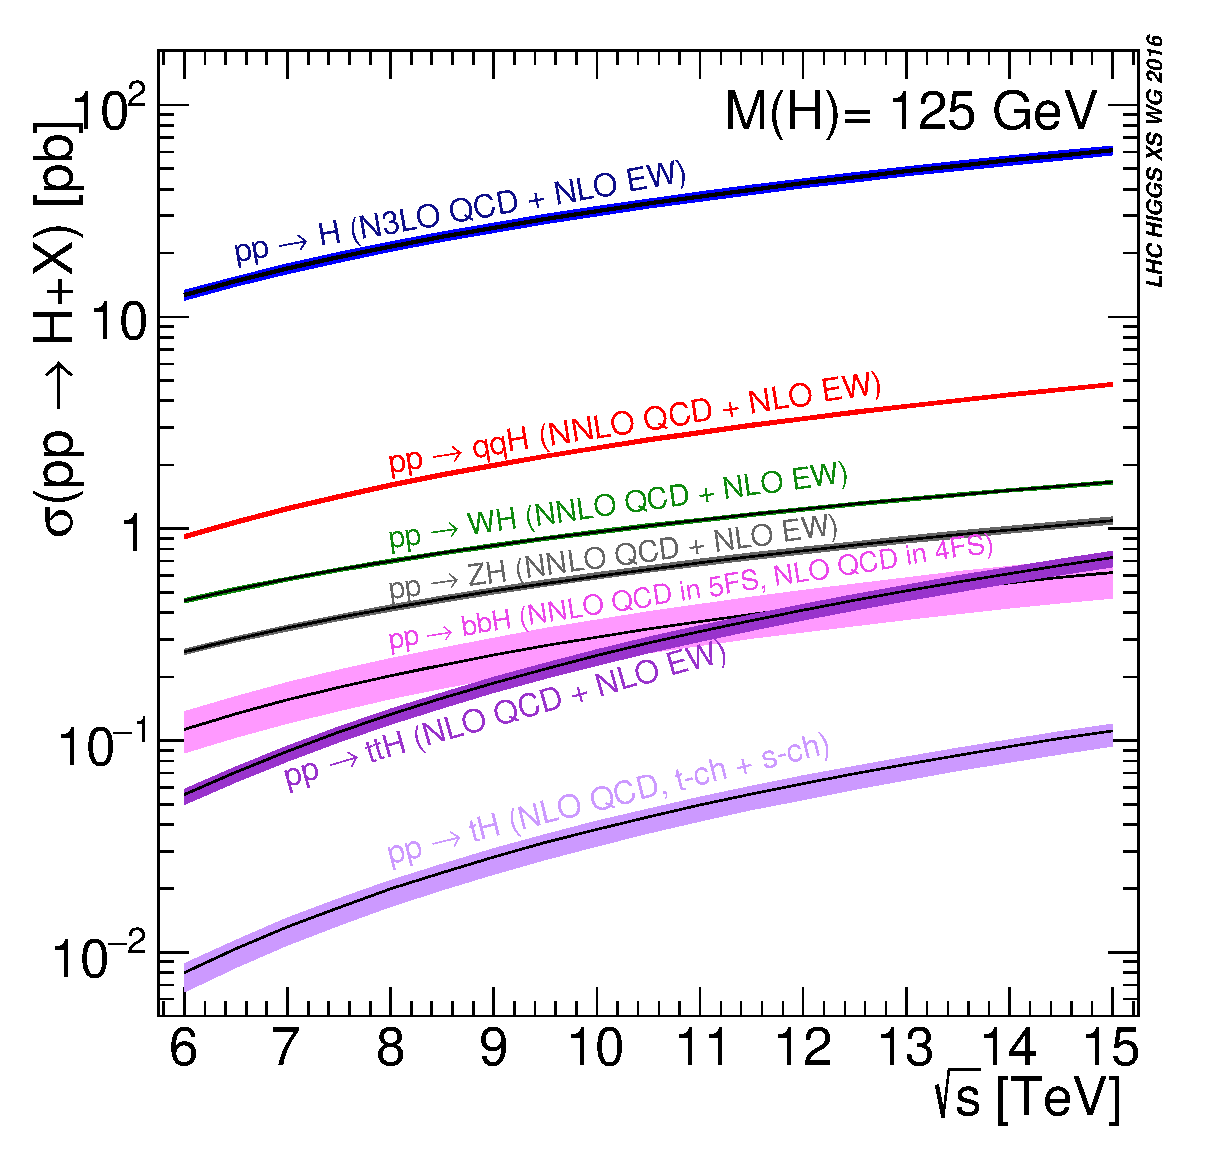
\includegraphics[width=0.5\textwidth]{theory/Higgs_XS_7-14TeV-2016.eps}
 \caption[The Standard Model Higgs boson production cross sections as a function of the center-of-mass energy, $\sqrt{s}$, for $pp$ collisions.]{%
  The Standard Model Higgs boson production cross sections as a function of the center-of-mass energy, $\sqrt{s}$, for $pp$ collisions.
  The VBF process is indicated as $qqH$.
  The theoretical uncertainties are indicated as bands~\cite{PDG2018:Ch11}.}
 \label{fig:Higgs_production_cross_section_theory}
\end{figure}

The SM Higgs has couplings to all the massive vector gauge fields and charged fermions, and so can decay into all of their particles.
At leading order the Higgs will decay primarily to a pair of $b$-quarks $(b\bar{b})$, a pair of weak vector bosons with one of them being off-shell $(VV^{*})$, a pair of gluons $(gg)$, a pair of tau leptons $(\tau^{+}\tau^{-})$, or a pair of photons $(\gamma\gamma)$.
The decays to massless gauge bosons (gluons and photons) are facilitated through loops of massive particles.
The Feynman diagrams for these decays are shown in \Cref{fig:Higgs_decay_channels}, listed in descending (observed) branching ratio in \Cref{table:Higgs_BRs}, and plotted with theory uncertainties in \Cref{fig:Higgs_BRs}.
As the Higgs Yukawa couplings are proportional to the mass of the decay products, it is seen that the Higgs primarily decays to $b\bar{b}$ as $m_{H} < 2 m_{t}$.
However, as hadron colliders mostly produce multijet events%
\footnote{Discovery machines are a messy business.}
from QCD processes, identifying jets coming from resonant $H \to b\bar{b}$ events is quite challenging.

Through the combination of results from the ATLAS and CMS experiment collaborations using approximately $5~\ifb$ of LHC Run 1 data~\cite{Pieri:2016szr}, experimental measurements of the Standard Model Higgs production cross-sections and decay modes have been made, as seen in \Cref{fig:combined_experiment_production_cross_sections}, \Cref{fig:combined_experiment_decay_BRs}, and \Cref{fig:combined_experiment_sigma_BR}.
It is seen that given the uncertainties on the measurements there is generally good agreement between the predictions of the Standard Model and experimental measurements, with all best fit values within two standard deviations of the SM predictions.

\begin{figure}[htbp]
 \centering
 \begin{subfigure}[t]{0.48\textwidth}
  \centering
  \includegraphics[width=\textwidth]{theory/Hbb.pdf}
  \caption[Feynman diagram for Higgs decay to $b\bar{b}$.]{%
   Feynman diagram for Higgs decay to $b\bar{b}$.}
  \label{fig:H_to_bb}
 \end{subfigure}
 \quad
 \begin{subfigure}[t]{0.48\textwidth}
  \centering
  \includegraphics[width=\textwidth]{theory/H_WW.pdf}
  \caption[Feynman diagram for Higgs decay to $WW^{*}$.]{%
   Feynman diagram for Higgs decay to $WW^{*}$.}
  \label{fig:H_to_WW}
 \end{subfigure}

 \begin{subfigure}[t]{0.48\textwidth}
  \centering
  \includegraphics[width=\textwidth]{theory/Hgg.pdf}
  \caption[Feynman diagram for Higgs decay to $gg$.]{%
   Feynman diagram for Higgs decay to $gg$.}
  \label{fig:H_to_gg}
 \end{subfigure}
 \quad
 \begin{subfigure}[t]{0.48\textwidth}
  \centering
  \includegraphics[width=\textwidth]{theory/Htautau.pdf}
  \caption[Feynman diagram for Higgs decay to $\tau^{+}\tau^{-}$.]{%
   Feynman diagram for Higgs decay to $\tau^{+}\tau^{-}$.}
  \label{fig:H_to_tautau}
 \end{subfigure}

 \begin{subfigure}[t]{0.48\textwidth}
  \centering
  \includegraphics[width=\textwidth]{theory/H_ZZ.pdf}
  \caption[Feynman diagram for Higgs decay to $ZZ^{*}$.]{%
   Feynman diagram for Higgs decay to $ZZ^{*}$.}
  \label{fig:H_to_ZZ}
 \end{subfigure}
 \quad
 \begin{subfigure}[t]{0.48\textwidth}
  \centering
  \includegraphics[width=\textwidth]{theory/H_photons.pdf}
  \caption[Feynman diagram for Higgs decay to $\gamma\gamma$.]{%
   Feynman diagram for Higgs decay to $\gamma\gamma$.}
  \label{fig:H_to_photons}
 \end{subfigure}
 \caption[The leading decay channels of the Higgs boson.]{%
  The leading decay channels of the Higgs boson.}
 \label{fig:Higgs_decay_channels}
\end{figure}

\begin{table}[htpb]
 \centering
 \caption[The branching ratios and the relative uncertainty for a Standard Model Higgs boson with $m_{H}=125~\GeV$.]^{+3.2\%}$ \\
  \addlinespace[0.3em]
  $H\to W^{+}W^{-}$       & $2.14 \times 10^{-1}$ & $_{-4.2\%}^{+4.3\%}$ \\
  \addlinespace[0.3em]
  $H\to \tau^{+}\tau^{-}$ & $6.27 \times 10^{-2}$ & $_{-5.7\%}^{+5.7\%}$ \\
  \addlinespace[0.3em]
  $H\to ZZ$               & $2.62 \times 10^{-2}$ & $_{-4.1\%}^{+4.3\%}$ \\
  \addlinespace[0.3em]
  $H\to \gamma\gamma$     & $2.27 \times 10^{-3}$ & $_{-4.9\%}^{+5.0\%}$ \\
  \addlinespace[0.3em]
  $H\to Z\gamma$          & $1.53 \times 10^{-3}$ & $_{-8.9\%}^{+9.0\%}$ \\
  \addlinespace[0.3em]
  $H\to \mu^{+}\mu^{-}$   & $2.18 \times 10^{-4}$ & $_{-5.9\%}^{+6.0\%}$ \\
  \bottomrule
 \end{tabular}\label{table:Higgs_BRs}%
\end{table}

\begin{figure}
 \centering
 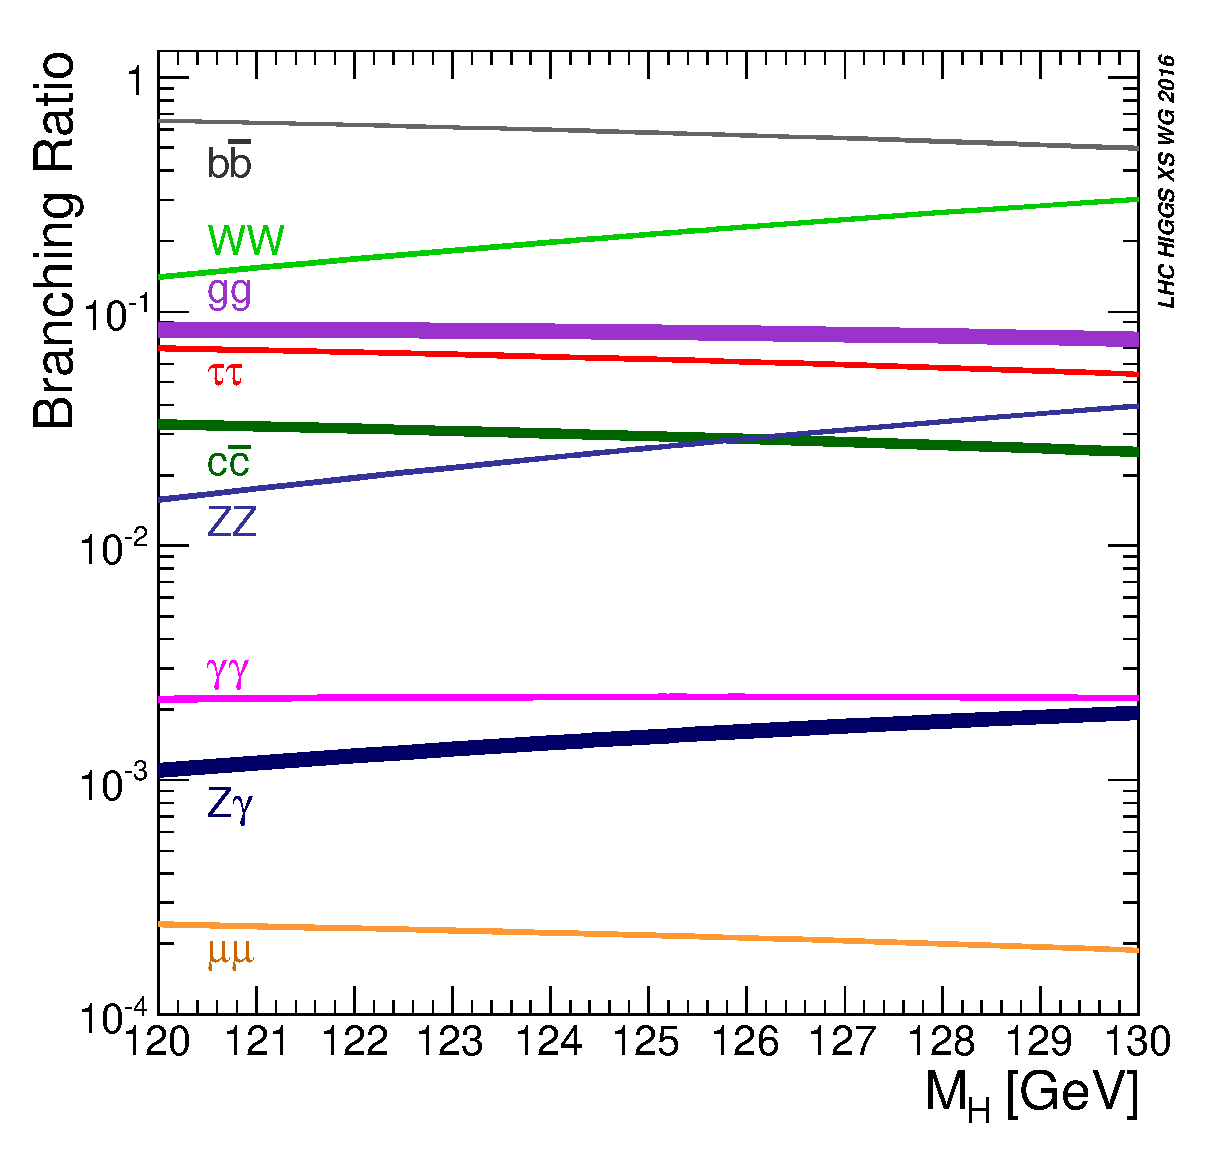
\includegraphics[width=0.5\textwidth]{theory/SMHiggsBR.eps}
 \caption[The branching ratios for the main decays of the Standard Model Higgs boson near $m_{H}=125~\GeV$.]{%
  The branching ratios for the main decays of the Standard Model Higgs boson near $m_{H}=125~\GeV$.
  The theoretical uncertainties are indicated as bands~\cite{PDG2018:Ch11}.}
 \label{fig:Higgs_BRs}
\end{figure}

\begin{figure}[htbp]
 \centering
 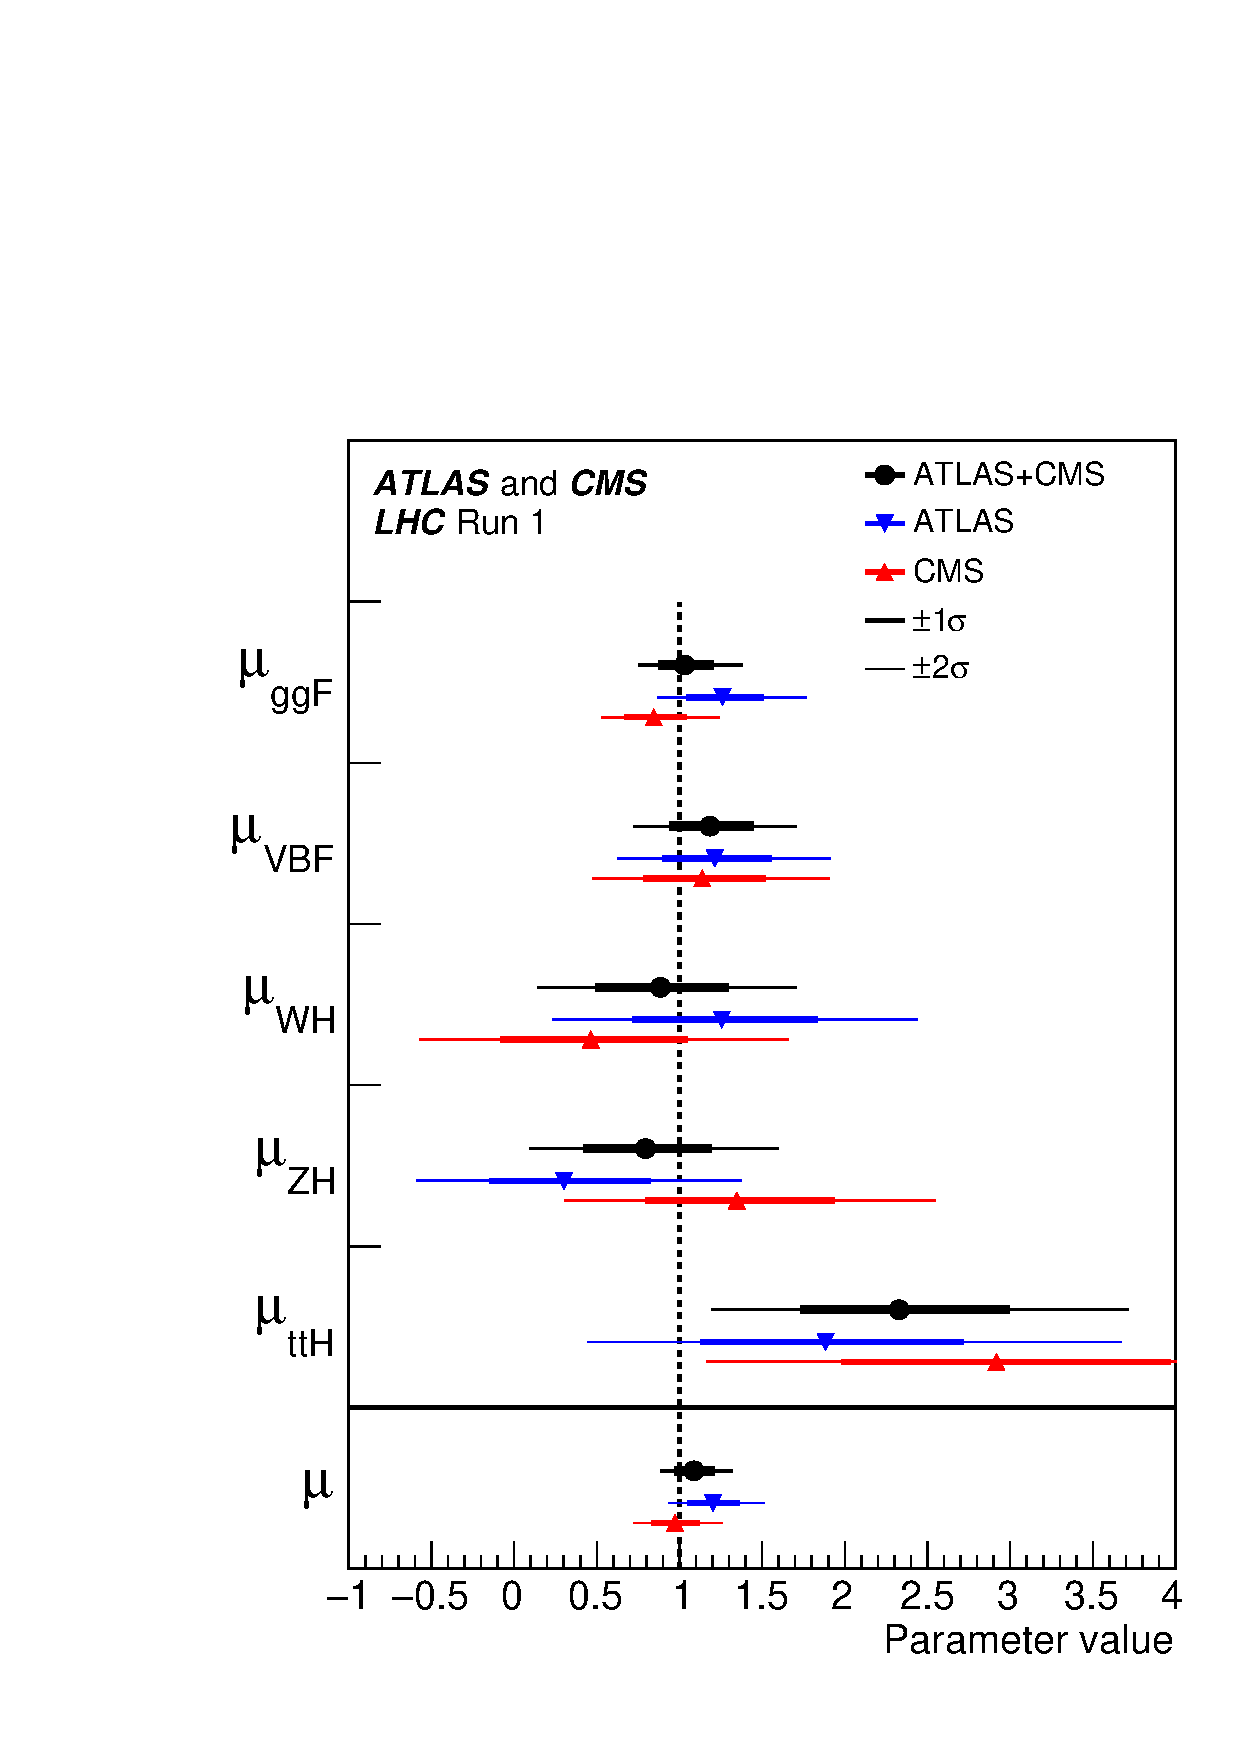
\includegraphics[width=0.5\textwidth]{theory/combined_experiment_production_cross_sections.pdf}
 \caption[Best fit results for the production signal strengths for the Standard Model Higgs boson for the combination of ATLAS and CMS data.]{%
  Best fit results for the production signal strengths for the Standard Model Higgs boson for the combination of ATLAS and CMS data.
  Also shown are the results from each experiment.
  The uncertainty bars indicate the $1\,\sigma$ (thick lines) and $2\,\sigma$ (thin lines) intervals.
  The measurements of the global signal strength $\mu$ are also shown~\cite{Pieri:2016szr}.}
 \label{fig:combined_experiment_production_cross_sections}
\end{figure}

\begin{figure}[htbp]
 \centering
 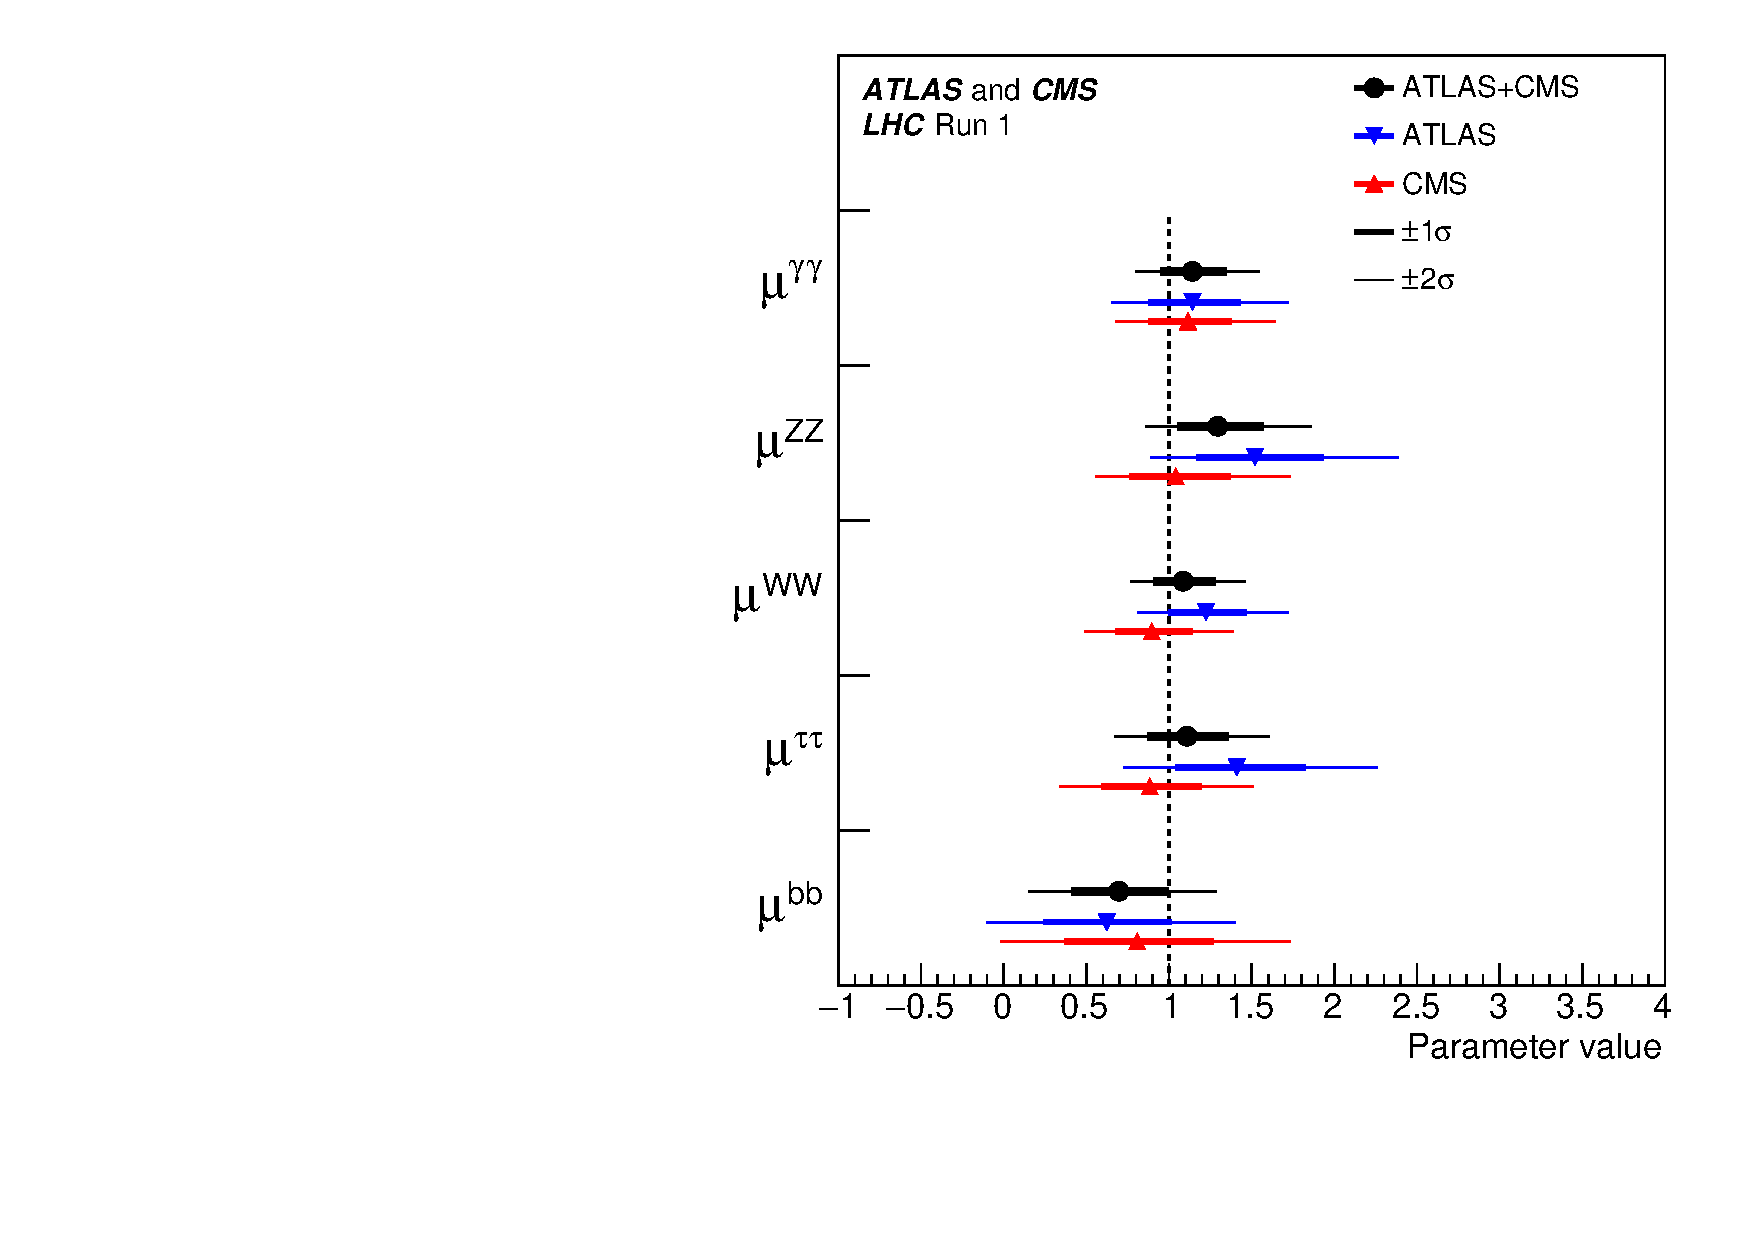
\includegraphics[width=0.45\textwidth]{theory/combined_experiment_decay_BRs.pdf}
 \caption[Best fit results for the decay signal strengths for the Standard Model Higgs boson for the combination of ATLAS and CMS data.]{%
  Best fit results for the decay signal strengths for the Standard Model Higgs boson for the combination of ATLAS and CMS data.
  Also shown are the results from each experiment.
  The uncertainty bars indicate the $1\,\sigma$ (thick lines) and $2\,\sigma$ (thin lines) intervals~\cite{Pieri:2016szr}.}
 \label{fig:combined_experiment_decay_BRs}
\end{figure}

\begin{figure}[htbp]
 \centering
 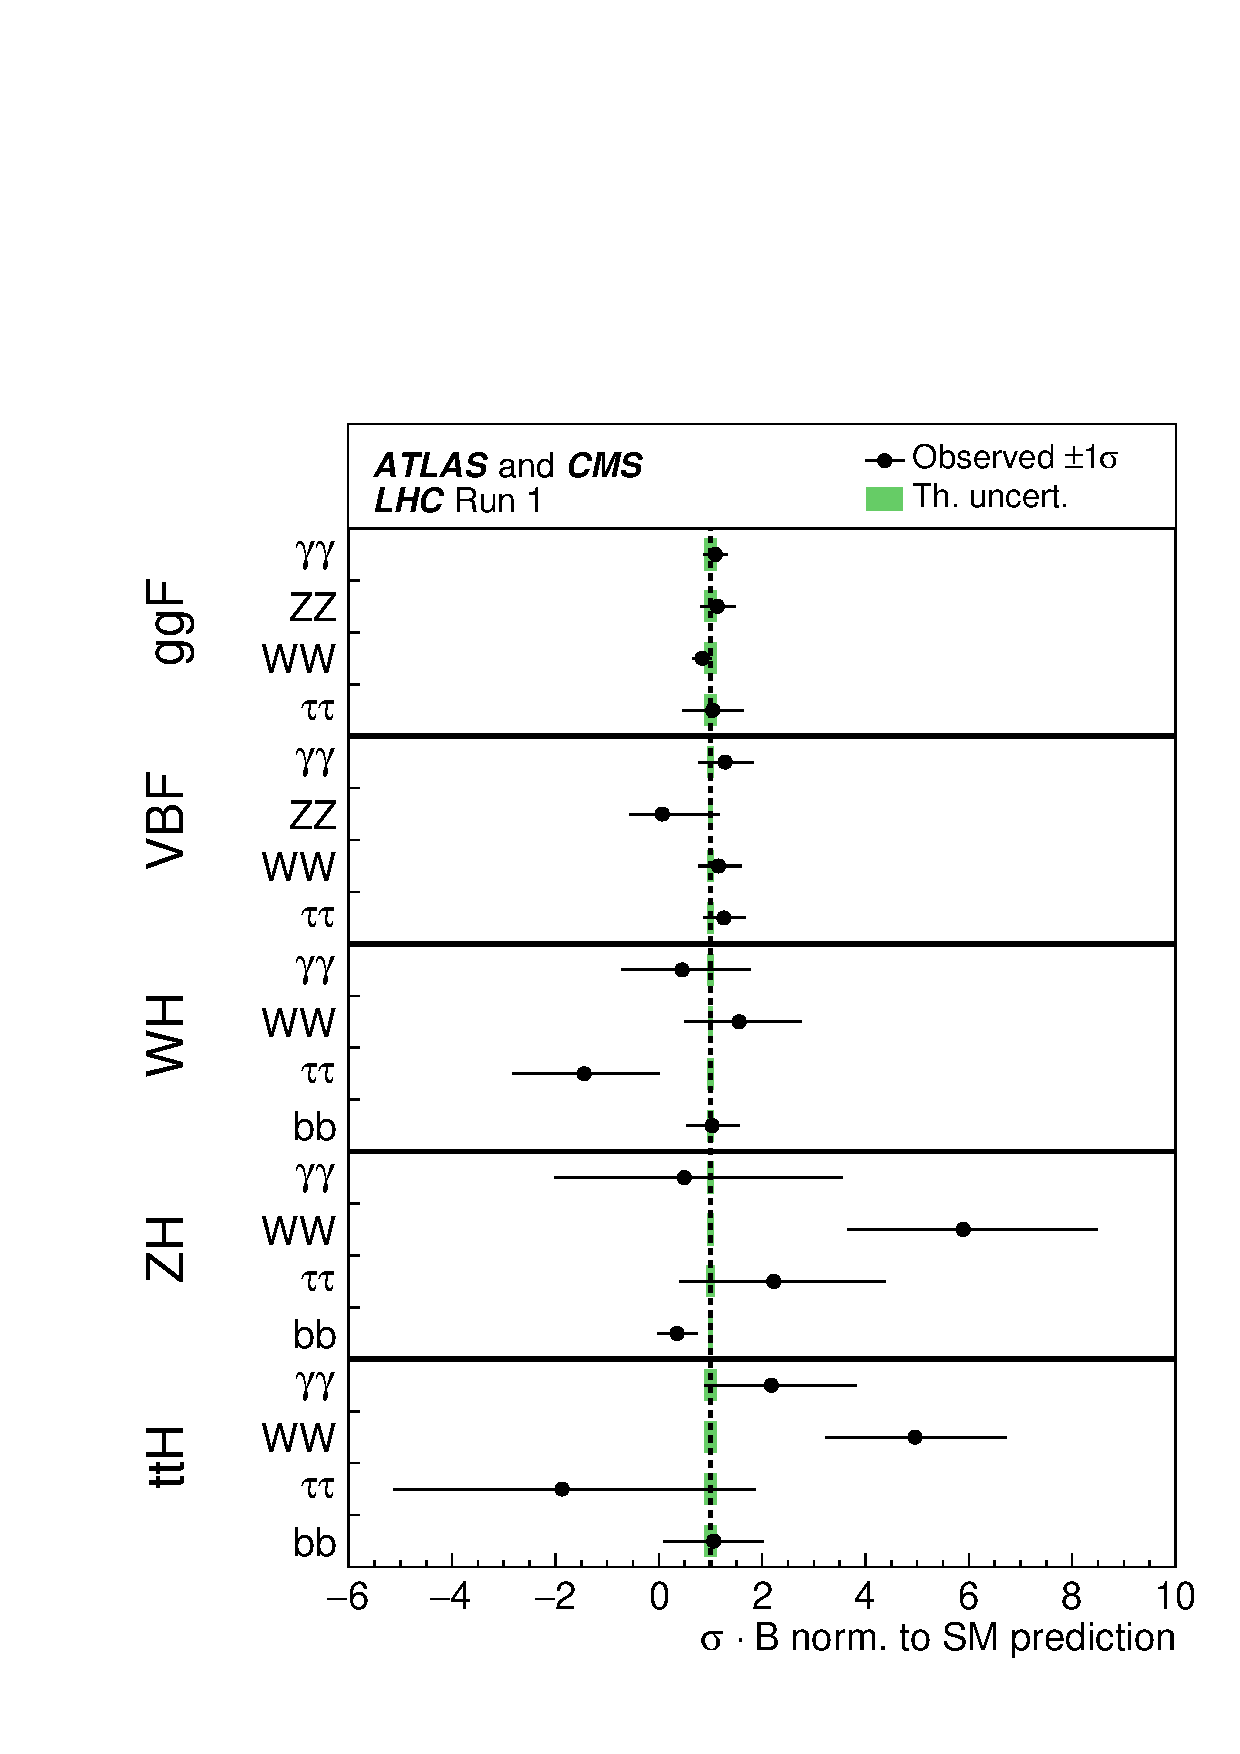
\includegraphics[width=0.45\textwidth]{theory/combined_experiment_sigma_BR.pdf}
 \caption[Best fit values of $\sigma_{i} \cdot B^{f}$ for each specific channel $i \to H \to f$, as obtained from the generic parameterization with 23 parameters for the combination of ATLAS and CMS measurements.]{%
  Best fit values of $\sigma_{i} \cdot B^{f}$ for each specific channel $i \to H \to f$, as obtained from the generic parameterization with 23 parameters for the combination of ATLAS and CMS measurements.
  The uncertainty bars indicate the $1\,\sigma$ intervals.
  The fit results are normalized to the SM predictions for the various parameters and the shaded bands indicate the theoretical uncertainties in these predictions.
  Only 20 parameters are shown because some are either not measured with a meaningful precision, in the case of the $H \to ZZ$ decay channel for the $WH$, $ZH$, and
  $ttH$ production processes, or not measured at all and therefore fixed to their corresponding SM predictions, in the case of the $H \to b\bar{b}$ decay mode for the ggF and VBF production processes~\cite{Pieri:2016szr}.}
 \label{fig:combined_experiment_sigma_BR}
\end{figure}

\clearpage
\section{Extensions to the Standard Model}

From astronomical observations of the rotation speeds of galaxies~\cite{Rubin:1970zza,Begeman:1991iy}, precision measurements of the cosmic microwave background~\cite{2013ApJS:darkmatter,Akrami:2018vks}, and gravitational lensing measurements~\cite{Trimble:10.1146,Bertone:2004pz,Feng:2010gw}, there is evidence that in addition to the normal matter of the Standard Model in the Universe there exists ``dark matter'' (DM) that constitutes approximately $26.8\%$ of the energy density of the Universe.
Dark matter is so far seen to interact with normal matter only through gravitation.
As it does not interact with normal matter through the electroweak or strong nuclear force, any interactions with normal matter are outside of the Standard Model.

To incorporate a model of particle dark matter there are a number of existing extensions of the Standard Model.
Among these are frameworks of simplified dark matter models~\cite{EXOT-2017-32,Jacques:2016dqz,Kahlhoefer:2015bea,Alves:2015pea} where new particles mediate the interactions of dark matter, $\chi$, with the Standard Model particles.
Among these are models for a single neutral vector mediator particle: a $\Zprime$.
One simple extension of the Standard Model is a vector or axial-vector simplified model through an additional $\mathrm{U}(1)$ gauge symmetry which gives dark matter particles a charge of this symmetry group~\cite{Abercrombie:2015wmb}, and results in either a vector $\left(\Zprime_{V}\right)$ or axial-vector $\left(\Zprime_{A}\right)$ boson mediator.
This model introduces five new parameters: the mass of the mediator, $m_{\Zprime}$, the mass of the Dirac fermion dark matter particle, $m_{\chi}$, the flavor-universal coupling of the $\Zprime$ to SM quarks, $g_{q}$, the coupling of the $\Zprime$ to all lepton flavors, $g_{\ell}$, and the coupling of the $\Zprime$ to dark matter, $g_{\chi}$.
The resulting interactions of the $\Zprime$ mediator and the particles are shown in \Cref{fig:Zprime_interactions}.

\begin{figure}[htbp]
 \centering
 \begin{subfigure}[t]{0.48\textwidth}
  \centering
  \includegraphics[width=\textwidth]{theory/Zprime_SM_coupling.pdf}
  \caption[Feynman diagram of the interactions of the $\Zprime$ mediator with Standard Model fermions.]{%
   Feynman diagram of the interactions of the $\Zprime$ mediator with Standard Model fermions.}
  \label{fig:Zprime_SM_coupling}
 \end{subfigure}%
 \quad
 \begin{subfigure}[t]{0.48\textwidth}
  \centering
  \includegraphics[width=\textwidth]{theory/Zprime_DM_coupling.pdf}
  \caption[Feynman diagram of the interactions of the $\Zprime$ mediator with dark matter.]{%
   Feynman diagram of the interactions of the $\Zprime$ mediator with dark matter.}
  \label{fig:Zprime_DM_coupling}
 \end{subfigure}%
 \caption[Feynman diagrams of the interactions of the $\Zprime$ mediator with both Standard Model fermions and dark matter.]{%
  Feynman diagrams of the interactions of the $\Zprime$ mediator with both Standard Model fermions and dark matter.}
 \label{fig:Zprime_interactions}
\end{figure}

Models with non-zero values of $g_{\ell}$ only slightly increase the mediator width, but further unnecessarily restrict the model space~\cite{Abercrombie:2015wmb}.
To simplify the model and the analysis done in this thesis, only leptophobic $\left(g_{\ell}=0\right)$ $\Zprime$ models are then considered.
This model then introduces the additional term to the Lagrangian density for a vector model of
\[
 \Lagrangian_{\textrm{vector}} = g_{q} \sum_{q} Z^{\prime}_{\mu} \bar{q} \gamma^{\mu} q + g_{\chi} Z^{\prime}_{\mu} \bar{\chi} \gamma^{\mu} \chi
\]
and for an axial-vector model
\[
 \Lagrangian_{\textrm{axial-vector}} = g_{q} \sum_{q} Z^{\prime}_{\mu} \bar{q} \gamma^{\mu}\gamma^{5} q + g_{\chi} Z^{\prime}_{\mu} \bar{\chi} \gamma^{\mu}\gamma^{5} \chi
\]
where $q$ and $\chi$ are respectively the Dirac spinors for the SM quark and dark matter fields and $g_{q}$ is democratic with respect to all quark flavors.

In $t$-channel processes that occur in scattering of dark matter off atomic nuclei, seen in \Cref{fig:Zprime_direct_detection}, the spin-independent interaction cross section of the vector mediator model is enhanced by $A^{2}$, where $A$ is the number of nucleons in the nucleus, as the result of spin coherence effects~\cite{Buchmueller:2014yoa,Chala:2015ama,EXOT-2017-32}.
These processes are relevant in dark matter direct detection experiments such as LUX~\cite{Akerib:2013tjd} and XENON100~\cite{Aprile:2013doa}, where the dark matter candidate considered is a weakly interacting massive particle (WIMP) model with a $\Zprime$ mediator.
For these experiments, the spin enhancement in the spin-independent model provides a limit more than $10^{4}$ stronger than the spin-dependent model limits, as seen for an example model with $g_{q} = 0.25$, $g_{\ell} = 0$, and $g_{\chi} = 1$ in \Cref{fig:direct_detection_exclusions}.
Similar results hold for the leptophilic models~\cite{EXOT-2017-32}.
Collider experiment searches exploit the $s$-channel process --- where there is no large spin dependence --- and as a result do not give competitive limits for vector mediator models, as seen in \Cref{fig:vector_model_exclusions}.
There is no large difference in collider detection sensitivity between vector and axial-vector mediator models, as seen in \Cref{fig:m_DM_vs_m_Zprime}.
However, for axial-vector models with $2 m_{\chi} > m_{\Zprime}$ there are unconstrained regions for low $\Zprime_{A}$ masses.
As a result, this thesis analysis considers an exotic signal search for only a low mass axial-vector leptophobic $\Zprime$ model in the high momentum regime to both further simplify the analysis and exploit similar analysis techniques developed for high momentum fully-hadronic decays of the Higgs boson.

\begin{figure}[htbp]
 \centering
 \includegraphics[width=0.4\textwidth]{theory/Zprime_direct_detection.pdf}
 \caption[Feynman diagram of the scattering of dark matter off Standard Model quarks through exchange of a $\Zprime$ mediator.]{%
  Feynman diagram of the $t$-channel scattering of dark matter, $\chi$, off Standard Model quarks, $q$, through exchange of a $\Zprime$ mediator.}
 \label{fig:Zprime_direct_detection}
\end{figure}

\begin{figure}[htbp]
 \centering
 \begin{subfigure}[t]{0.48\textwidth}
  \centering
  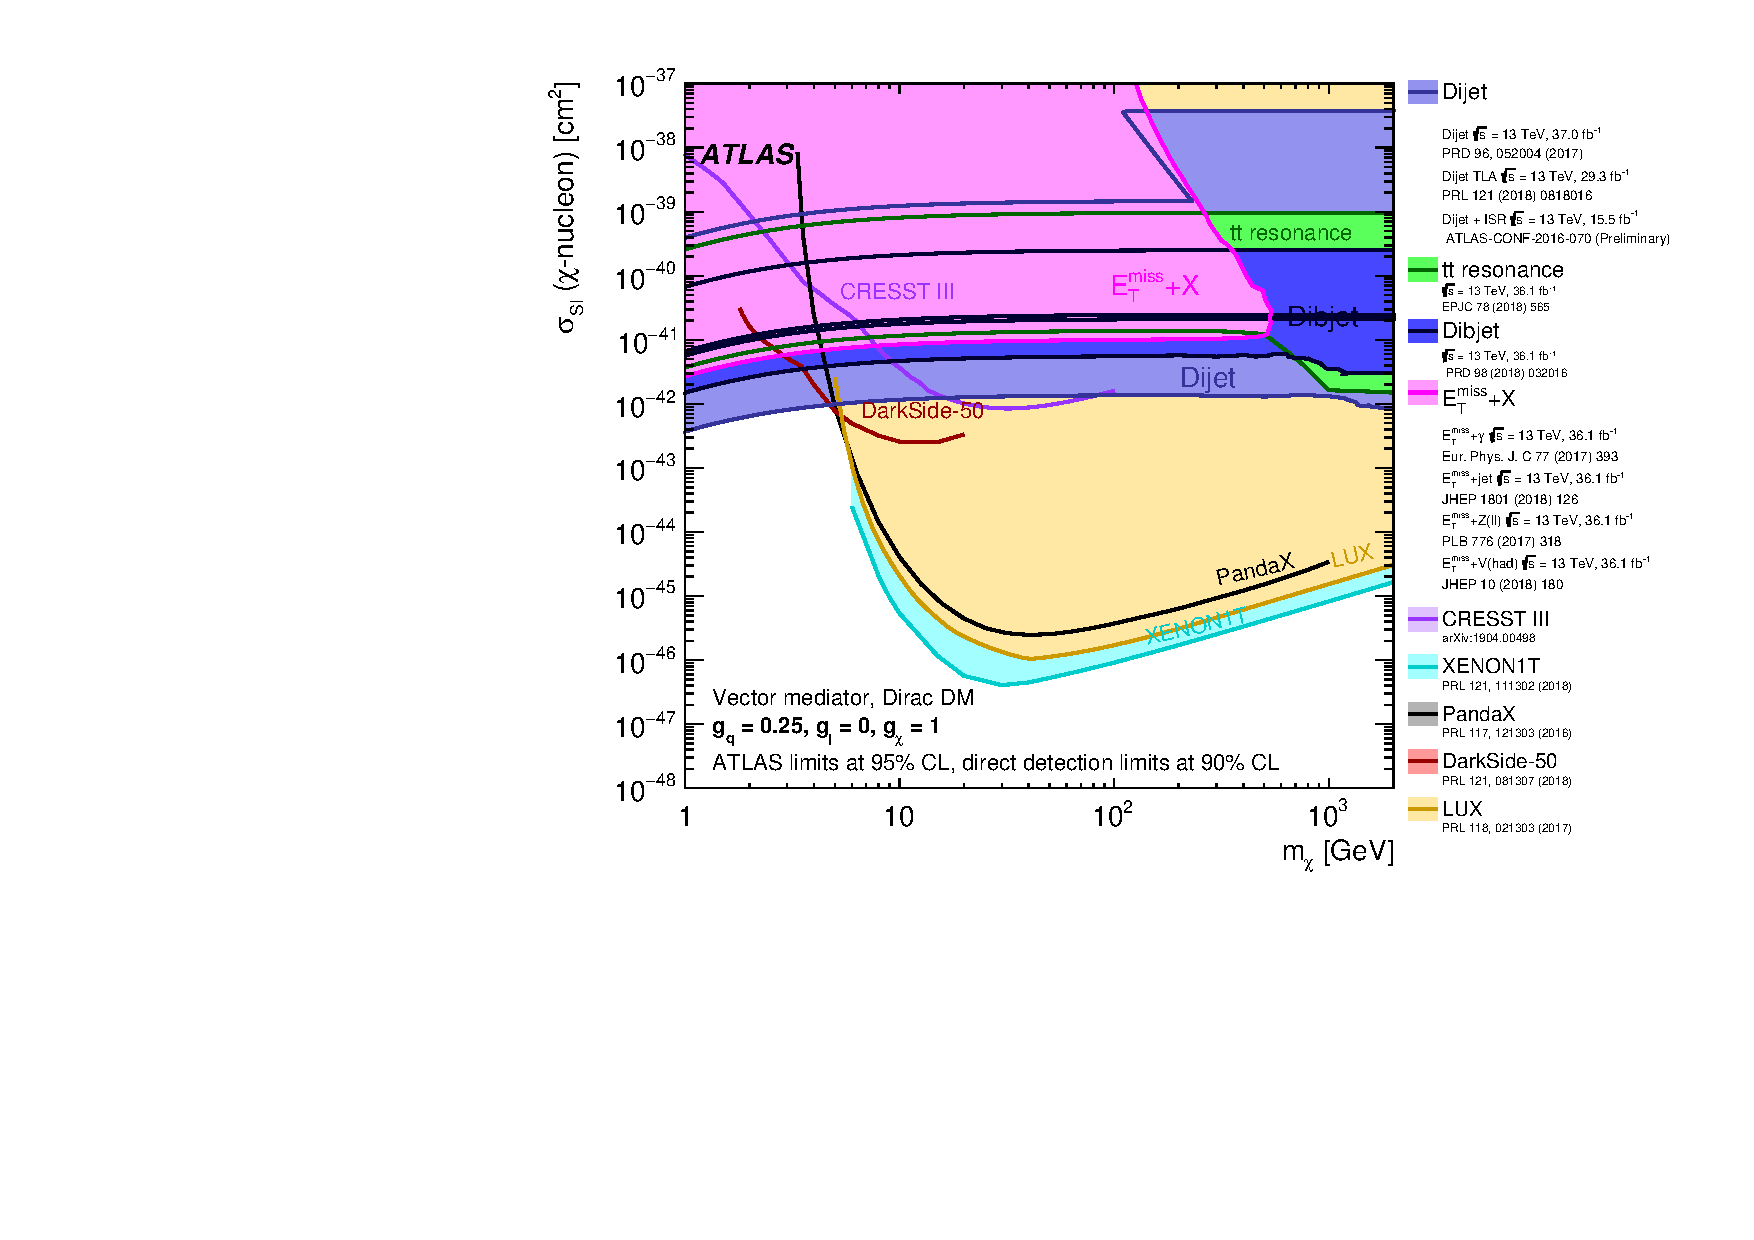
\includegraphics[width=\textwidth]{theory/vector_model_exclusions.pdf}
  \caption[Limits on the spin-independent WIMP--nucleon scattering cross section for a $\Zprime$ vector mediator model.]{%
   Limits on the spin-independent WIMP--nucleon scattering cross section for a $\Zprime$ vector mediator model.}
  \label{fig:vector_model_exclusions}
 \end{subfigure}%
 \quad
 \begin{subfigure}[t]{0.48\textwidth}
  \centering
  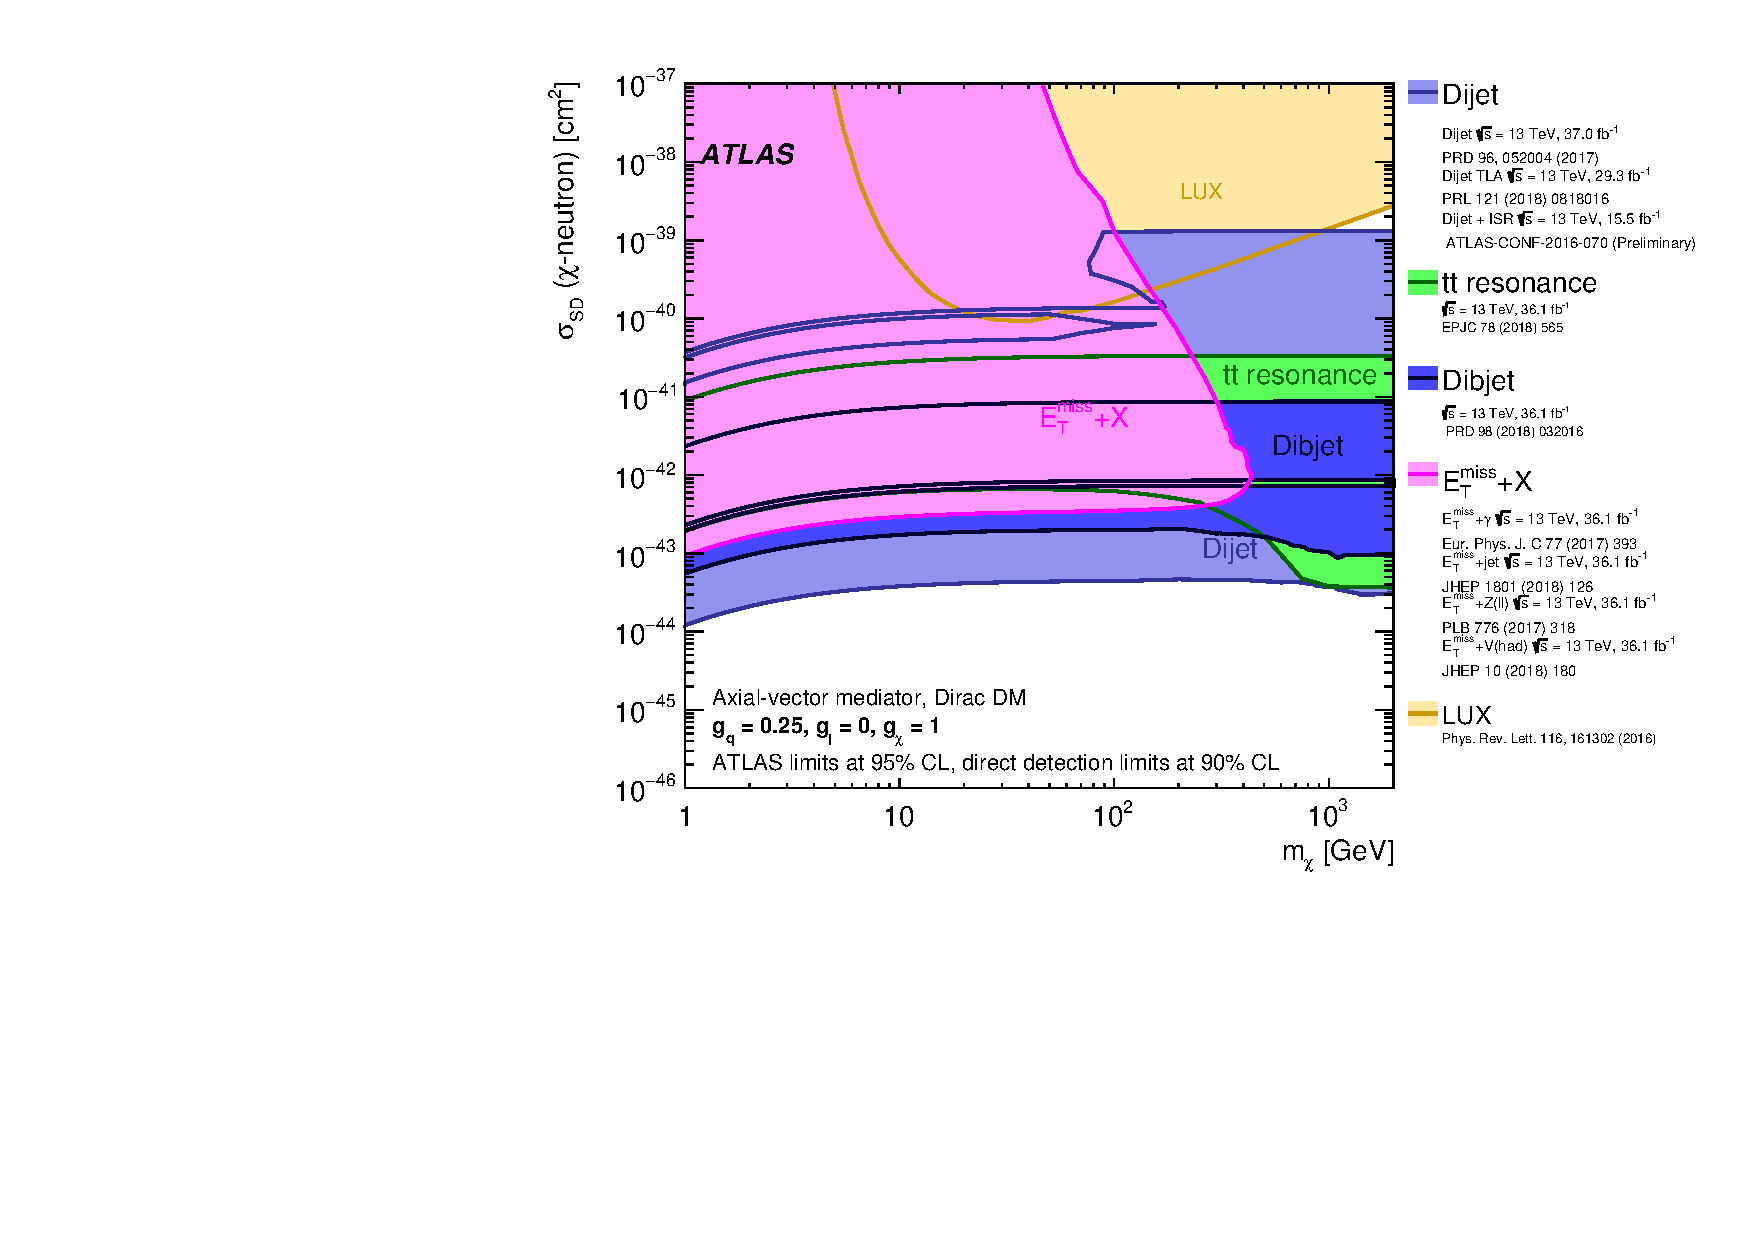
\includegraphics[width=\textwidth]{theory/axialvector_model_exclusions.pdf}
  \caption[Limits on the spin-dependent WIMP--neutron scattering cross section for a $\Zprime$ axial-vector mediator model.]{%
   Limits on the spin-dependent WIMP--neutron scattering cross section for a $\Zprime$ axial-vector mediator model.}
  \label{fig:axialvector_model_exclusions}
 \end{subfigure}%
 \caption[Comparison of inferred LHC experiment limits with the constraints from direct detection experiments on the WIMP--nucleon scattering cross section in the context of $\Zprime$ simplified model with $g_{q} = 0.25$, $g_{\ell} = 0$, and $g_{\chi} = 1$.]{%
  Comparison of inferred LHC experiment limits with the constraints from direct detection experiments on the WIMP--nucleon scattering cross section in the context of $\Zprime$ simplified model with $g_{q} = 0.25$, $g_{\ell} = 0$, and $g_{\chi} = 1$.
  LHC limits are shown at $95\%$ CL and direct detection limits at $90\%$ CL.
  The comparison is valid solely in the context of this model, assuming a mediator width fixed by the dark matter mass and the coupling values given.
  LHC searches and direct detection experiments exclude the shaded areas.
  Exclusions of smaller scattering cross sections do not imply that larger scattering cross sections are also excluded~\cite{EXOT-2017-32}.}
 \label{fig:direct_detection_exclusions}
\end{figure}

\begin{figure}[htbp]
 \centering
 \begin{subfigure}[t]{0.48\textwidth}
  \centering
  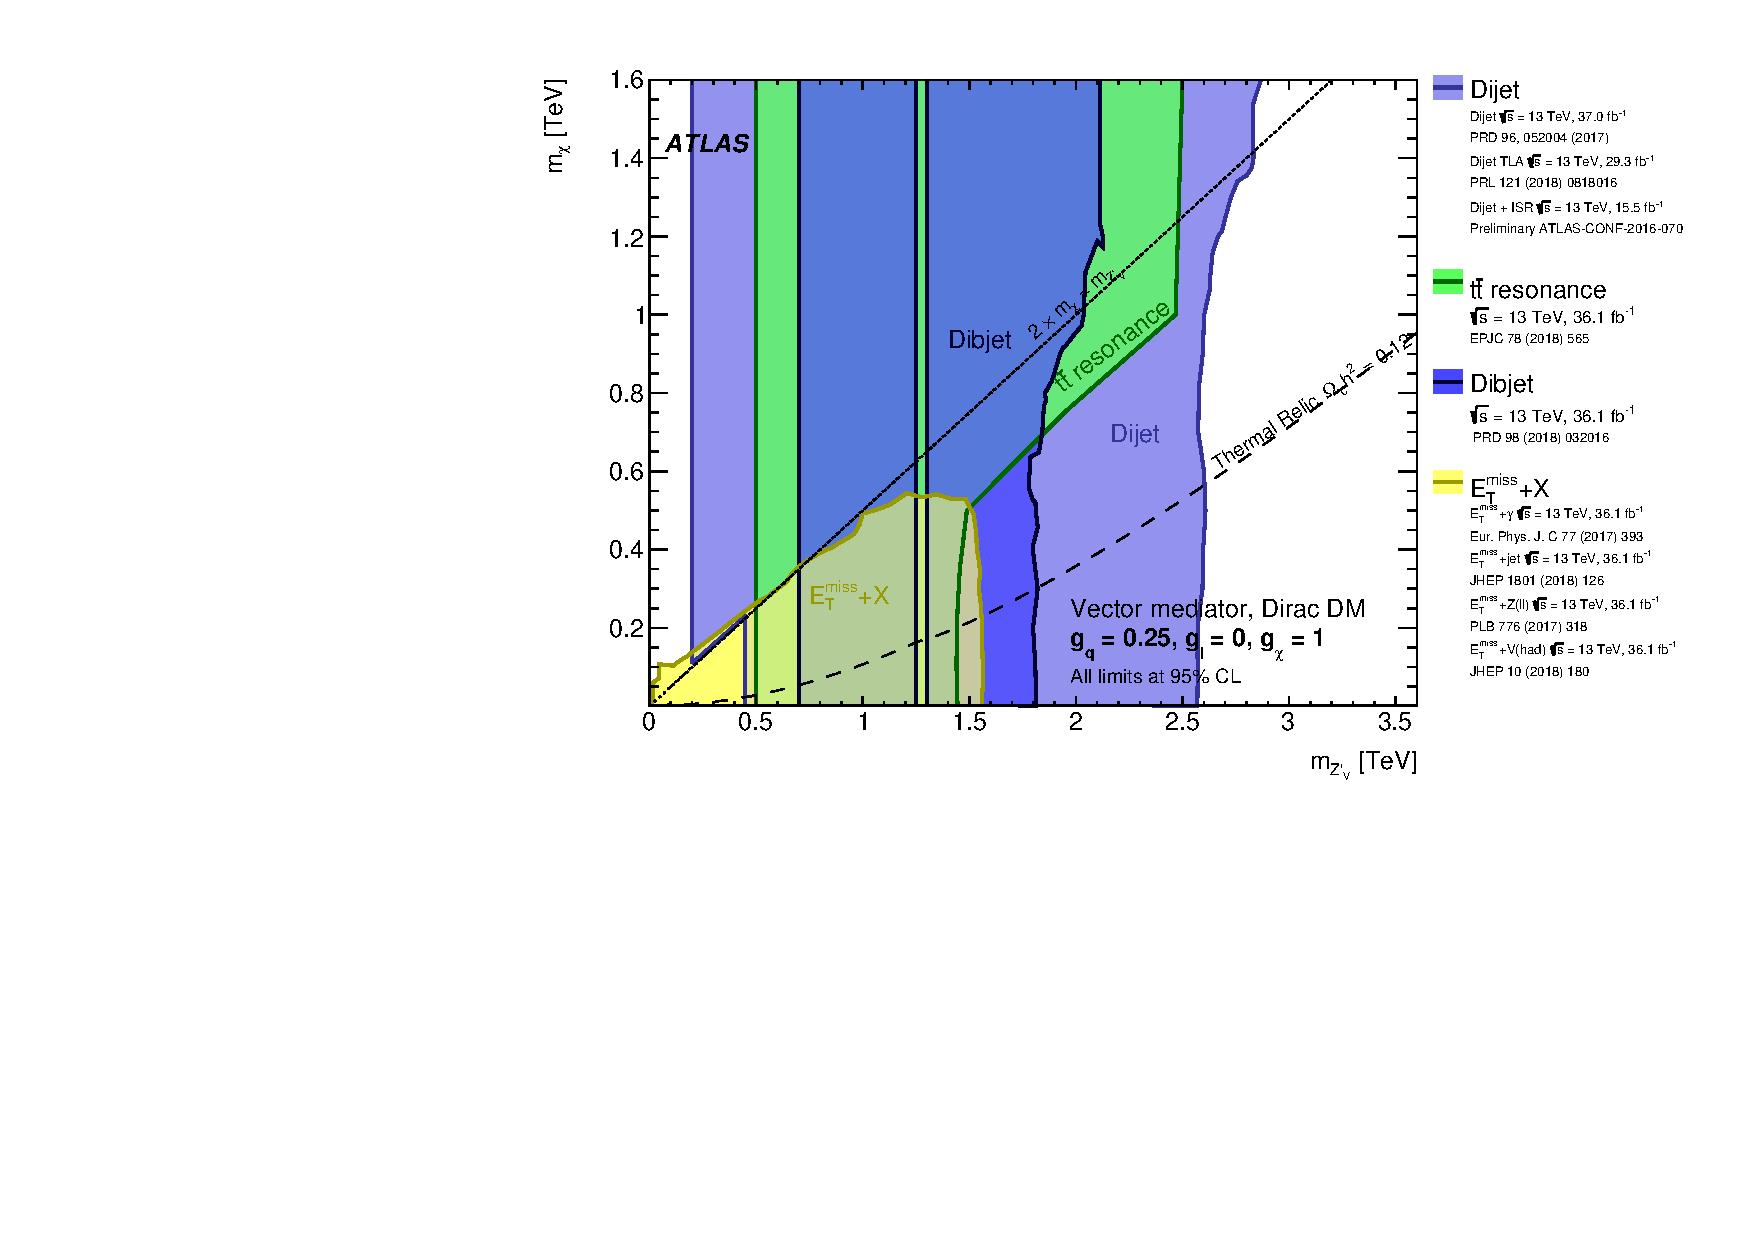
\includegraphics[width=\textwidth]{theory/m_DM_vs_m_ZprimeV.pdf}
  \caption[Exclusions for a $\Zprime$ vector mediator model.]{%
   Exclusions for a $\Zprime$ vector mediator model.
   Above the curve annihilation processes described by the simplified model deplete the density to $\Omega h^{2} < 0.12$.}
  \label{fig:m_DM_vs_m_ZprimeV}
 \end{subfigure}%
 \quad
 \begin{subfigure}[t]{0.48\textwidth}
  \centering
  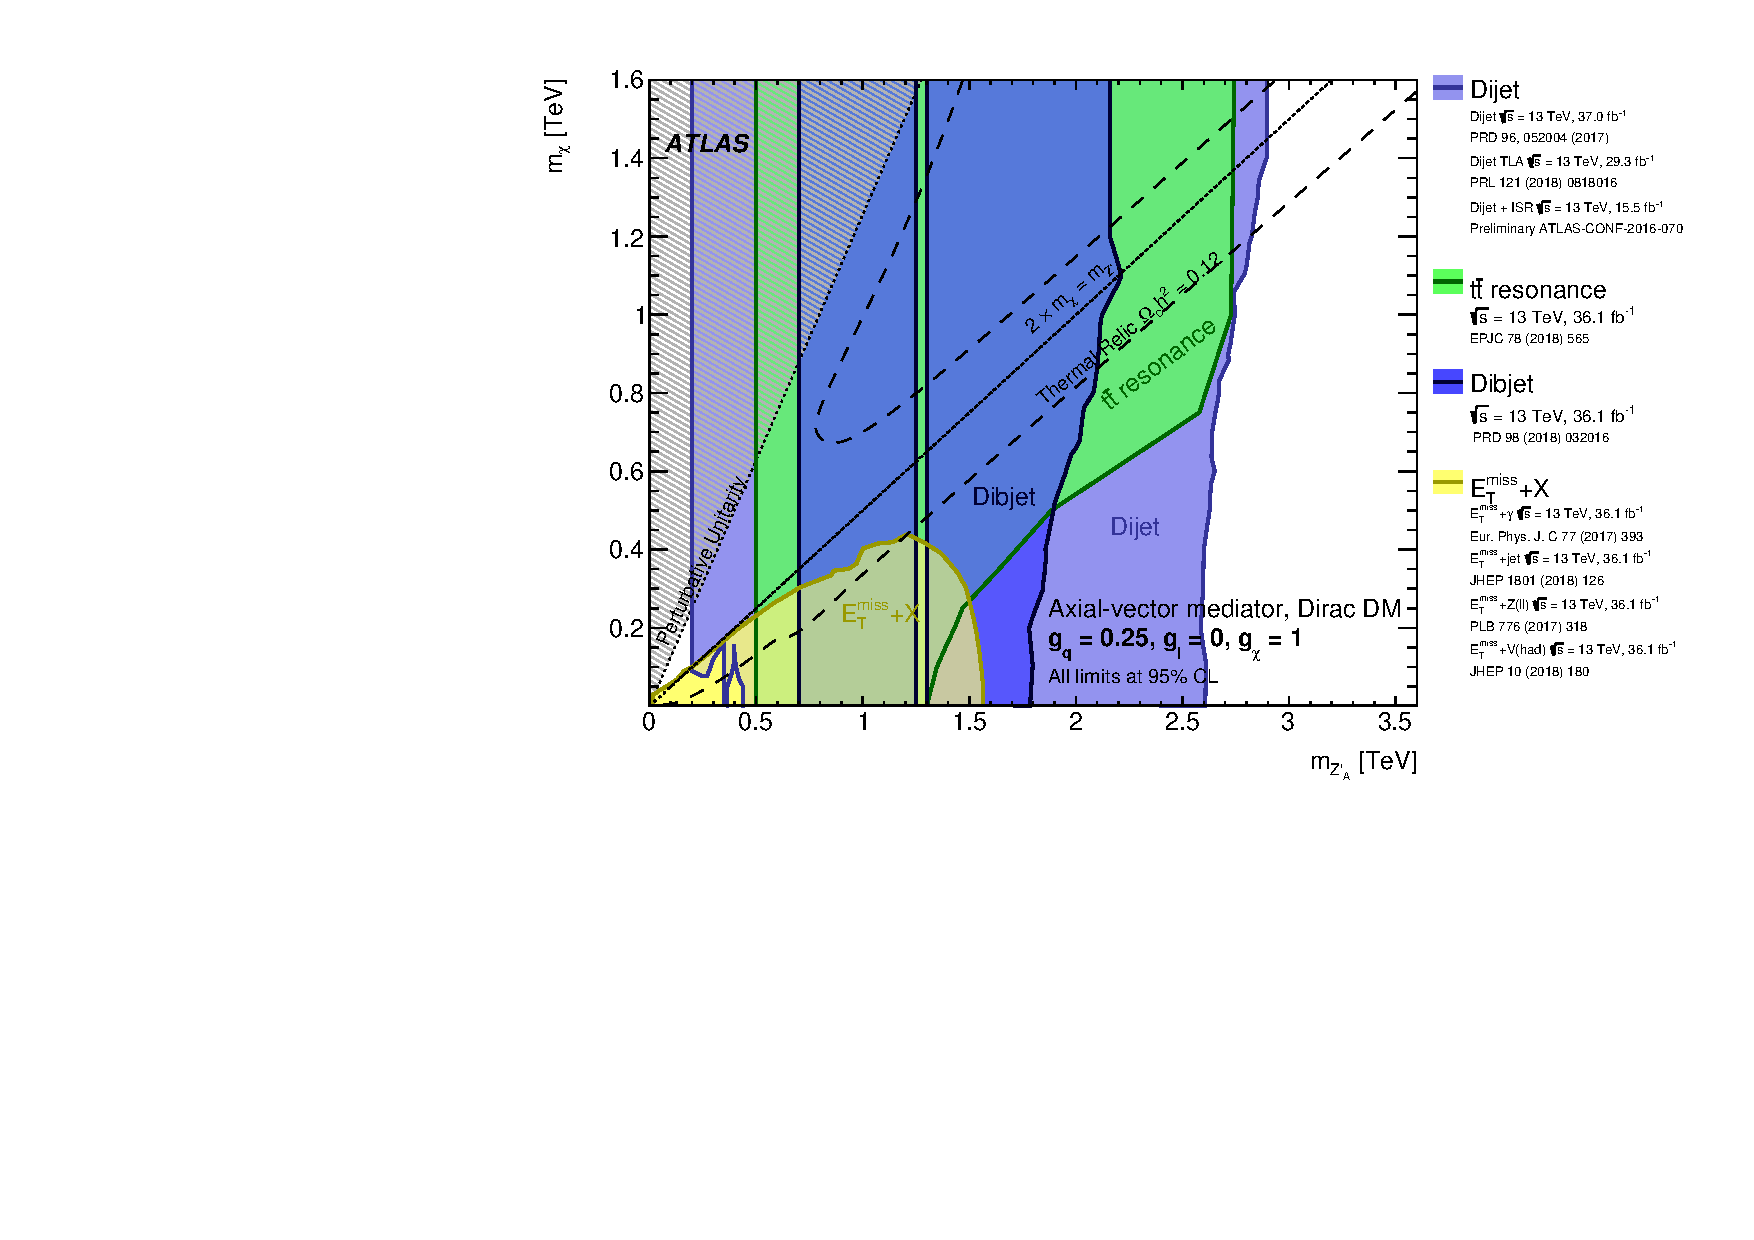
\includegraphics[width=\textwidth]{theory/m_DM_vs_m_ZprimeA.pdf}
  \caption[Exclusions for a $\Zprime$ axial-vector mediator model.]{%
   Exclusions for a $\Zprime$ axial-vector mediator model.
   Between the two curves annihilation processes described by the simplified model deplete the density to $\Omega h^{2} < 0.12$.}
  \label{fig:m_DM_vs_m_ZprimeA}
 \end{subfigure}%
 \caption[Regions in the (mediator-mass, DM-mass) plane excluded at $95\%$ CL by visible and invisible searches for leptophobic $\Zprime$ mediator simplified models with $g_{q} = 0.25$, $g_{\ell} = 0$, and $g_{\chi} = 1$.]{%
  Regions in the (mediator-mass, DM-mass) plane excluded at $95\%$ CL by visible and invisible searches for leptophobic $\Zprime$ mediator simplified models.
  The exclusions are computed for $g_{q} = 0.25$, $g_{\ell} = 0$, and $g_{\chi} = 1$.
  Dashed curves labeled ``thermal relic'' correspond to combinations of DM and mediator mass values that are consistent with a DM density of $\Omega h^{2} = 0.12$ and a standard thermal history~\cite{Baer:2014eja}, for dimensionless Hubble parameter $h$.
  The dotted line indicates the kinematic threshold where the mediator can decay on-shell into DM.
  Excluded regions that are in tension with the perturbative unitary considerations of~\cite{Kahlhoefer:2015bea} are indicated by shading in the upper left corner~\cite{EXOT-2017-32}.}
 \label{fig:m_DM_vs_m_Zprime}
\end{figure}


 \chapter{The Large Hadron Collider (LHC)}\label{chapter:LHC}

The Large Hadron Collider (\Gls{LHC}) at CERN is the world's most powerful superconducting hadron accelerator and collider.
It sits in the $26.7~\mathrm{km}$ tunnel originally housing CERN's Large Electron Position Collider (LEP) passing roughly $100~\mathrm{m}$ beneath the borders of Switzerland and France.
The LHC tunnels form an octagon with rounded corners consisting of eight arcs and eight straight sections that connect eight \glspl{interaction point} where the beam paths can be made to cross for collisions.
Four of those collision points are located at caverns that contain the main four experiments of the LHC: ATLAS~\cite{PERF-2007-01} at Point 1, CMS~\cite{CMS:2008} at Point 5, LHCb~\cite{LHCb:2008} at Point 8, and ALICE~\cite{ALICE:2008} at Point 2.
The other four interaction points are left intentionally unused for collisions and beam crossings are forgone to prevent unnecessary disruption of the beams~\cite{Evans:2008}.

\section{Design}

The LHC was designed to collide beams of protons at high energy with very high luminosity.
Its design center-of-mass energy is $14~\TeV{}$ and its design maximum instantaneous luminosity%
\footnote{In the more familiar units of barns used by particle physicists, $10^{34}~\mathrm{cm}^{-2}\mathrm{s}^{-1}=10~\mathrm{nb}^{-1}\mathrm{s}^{-1}=0.036~\mathrm{fb}^{-1}\mathrm{hr}^{-1}$.}
is $10^{34}~\mathrm{cm}^{-2}\mathrm{s}^{-1}$~\cite{Bruning:782076,Evans:2008}.
Given the extreme beam intensity required to reach such luminosities proton-anti-proton collisions (as was used successfully at Fermilab's Tevatron) are not feasible.
Instead, two counter-circulating beams of protons are used.
This imposes the requirement of opposite magnetic dipole fields in the rings.

The proton beams are guided along the LHC by a complex system of superconducting magnets.
The system consists of 1,232 $8.3~\mathrm{T}$ dipole magnets responsible for bending the beam and 392 $7.5~\mathrm{T}$ main quadrupole magnets dedicated to focusing the beam.
These are complemented by many insertion quadrupole magnets to help suppress beam dispersion~\cite{Rossi:2003,Rossi:2004}.
The high magnetic fields require huge currents, with the main dipole magnets designed for a nominal current of $11,600~\mathrm{A}$.
To deliver this much current while also staying superconducting the magnets are submerged in a liquid helium bath at $1.9~\mathrm{K}$ in a vacuum-sealed inner vessel, as seen in \Cref{fig:LHC_dipole_cross_section}.
The magnetic coils that carry this current are assembled at CERN from copper stabilized NbTi Rutherford cables, as shown for similar cables in~\cite{CERN-FOOTAGE-2016-014-001}.

\begin{figure}[htbp]
 \centering
 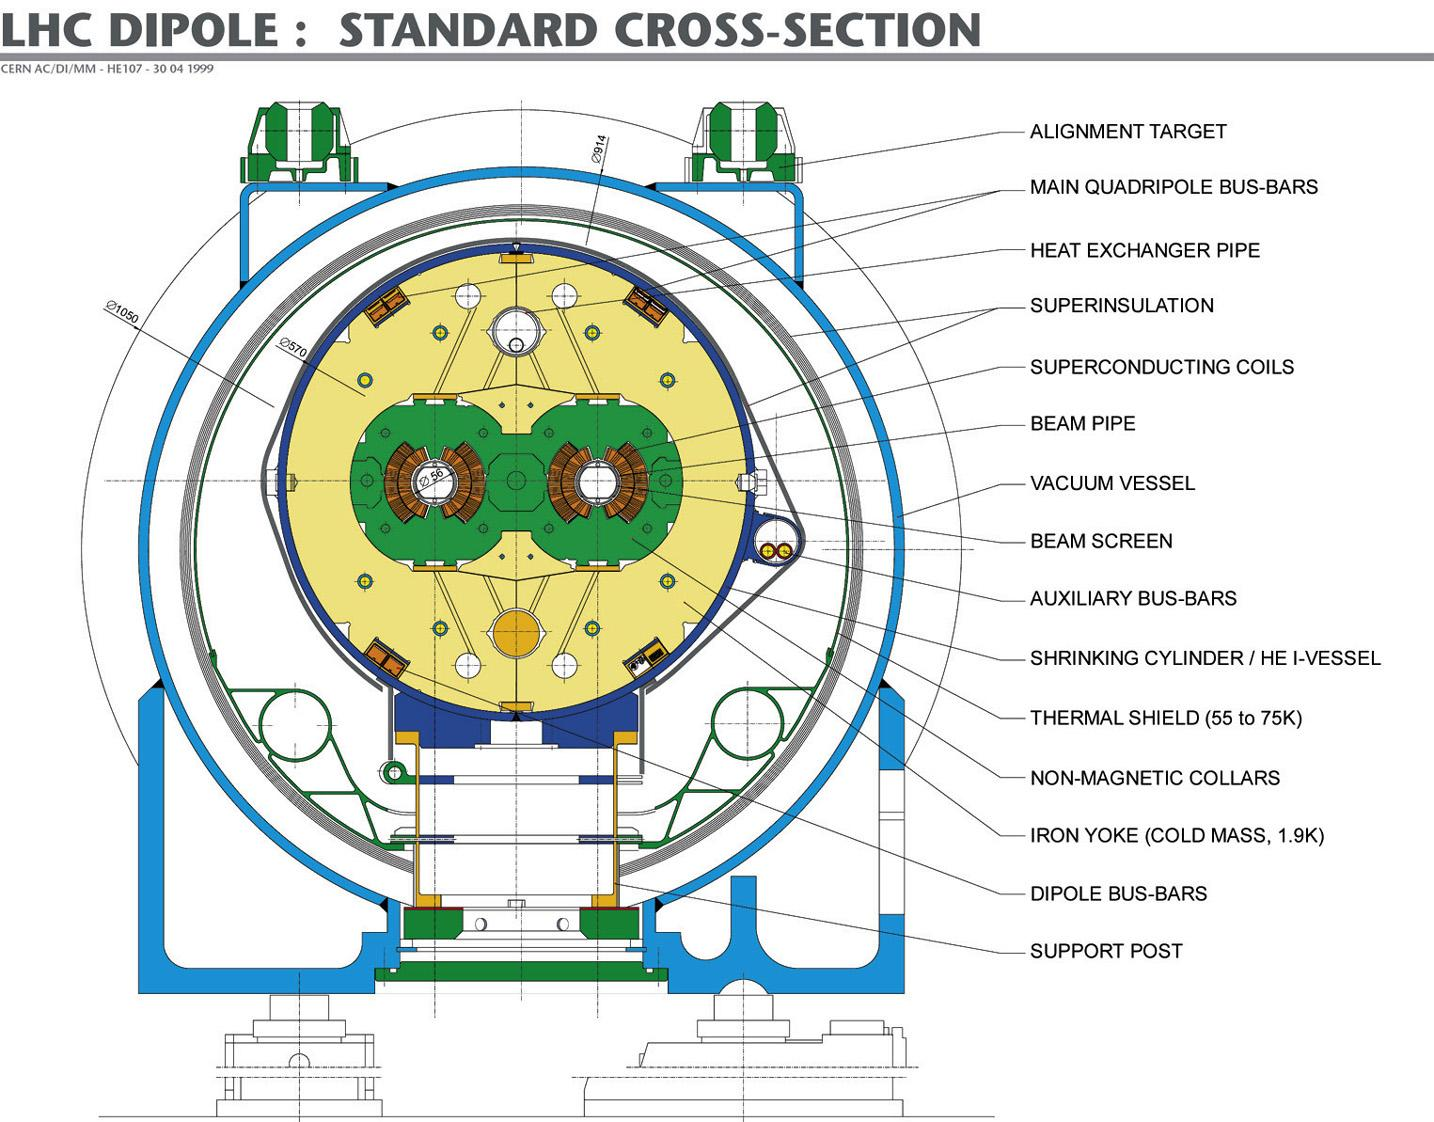
\includegraphics[width=0.6\textwidth]{LHC/LHC_dipole_cross_section.jpg}
 \caption[The cross-section of an LHC dipole magnet with cold mass and vacuum chamber.]{%
  The cross-section of an LHC dipole magnet with cold mass and vacuum chamber~\cite{LHC:dipole}.}\label{fig:LHC_dipole_cross_section}
\end{figure}

\section{Accelerator}

The LHC is the last step for protons in a sequence of accelerators, as shown in \Cref{fig:LHC_accelerator_complex}, that increase the energy of the beams.
The protons start from a single bottle of Hydrogen gas%
\footnote{This is the same bottle that has been used since the very start of LHC operations, and given that the LHC can be refilled hundreds of thousands of times from one $\textrm{ml}$ of Hydrogen, a typical industrial bottle of Hydrogen would last for over a billion years of LHC operations.}
at the site for the Linac2 linear accelerator.
The Hydrogen gas passes through an area of very high electrical field which ionizes the gas allowing for the electrons to be diverted away and for the protons to continue.
The protons then enter Linac2, the first accelerator of the LHC injector chain, where they are accelerated to an energy of $50~\MeV$.
The proton beam is then split and injected into the four Proton Synchrotron Booster rings where the beams are accelerated to $1.4~\GeV$ before recombination and injection into the \Gls{Proton Synchrotron} (PS) where the beam is further accelerated to $25~\GeV$ and forms a bunch train with $25~\textrm{ns}$ spacing --- radio frequency (RF) harmonics with bunches of protons surfing the RF wave troughs.
In the penultimate stage of the injector chain, the beam is injected into the Super Proton Synchrotron where it reaches an energy of $450~\GeV$.
Finally, the protons are injected into the LHC and split into two countercirculating beams.
Once the beams are circulating in the LHC they are further accelerated while keeping the $25~\textrm{ns}$ spacing.
They achieve their final energy of $6.5~\TeV$ by RF accelerator systems at Point 4~\cite{Evans:2008,Boussard:410377}.
The beams can circulate stably in the LHC for many hours and so only need to be refilled if the beam is dumped.

\begin{figure}[htbp]
 \centering
 \includegraphics[width=\textwidth]{LHC/LHC_accelerator_complex.jpg}
 \caption[Sketch of the CERN accelerator complex.]{%
  Sketch of the CERN accelerator complex.
  The LHC (dark grey ring) is the last ring in a complex chain of particle accelerators, where smaller machines are used in a chain to help boost particles to their final energies and provide beams to a whole set of smaller experiments~\cite{Haffner:1621894}.
  The LHC proton injector chain is the indicated by the paths marked with light grey arrows.}\label{fig:LHC_accelerator_complex}
\end{figure}

\section{Collider}\label{section:LHC_collider}

The circulating proton beams in the LHC cross paths at the four experimental interaction points where the main LHC experiments are located.
The collisions of the proton beams in the experiments have a resulting center-of-mass energy of $\sqrt{s} = 13~\TeV$ and, as shown by \Cref{eq:events_from_luminosity}, the number of events generated per second for a particular process is governed by the machine (instantaneous) luminosity, $\luminosity$, which for a beam shape that is Gaussian in profile is
\begin{equation}
 \luminosity = \frac{N_{b}^{2} n_{b} f_{\mathrm{rev}} \,\gamma_{r}}{4 \pi \epsilon_{n} \beta^{*}} F
 \label{eq:machine_luminosity}
\end{equation}
where $N_{b}$ is the number of particles per bunch, $n_{b}$ is the number of bunches per beam, $f_{\mathrm{rev}}$ is the revolution frequency, $\gamma_{r}$ is the relativistic gamma factor, $\epsilon_{n}$ is the normalized transverse beam emittance, $\beta^{*}$ is the beta function%
\footnote{The amplitude function is dependent on the bunch cross section, $\sigma$, and the transverse beam emittance, $\epsilon$, $\beta = \pi \sigma^{2}/\epsilon$~\cite{PDG2018:Ch30}.
 The beams are squeezed as they approach the interaction point, decreasing the amplitude such that $\beta^{*}$ is a smaller value of $\beta$ than at other points.}
(or ``amplitude function'') at the collision point, and $F$ is the geometric luminosity reduction factor due to the crossing angle at the interaction point:
\[
 F = \left(1 + \left(\frac{\theta_{c} \,\sigma_{z}}{2 \sigma^{*}}\right)\right)^{-1/2},
\]
where $\theta_{c}$ is the full crossing angle at the interaction point, $\sigma_{z}$ is the RMS bunch length, and $\sigma^{*}$ is the transverse RMS beam size at the interaction point~\cite{Evans:2008}.
Nominal design values for these quantities are given in \Cref{table:LHC_collider_parameters}, which additionally shows the incredibly successfully results of the LHC operations and accelerator teams' operation of the LHC in Run II.
From \Cref{eq:events_from_luminosity} and \Cref{eq:machine_luminosity} it is seen that to obtain the high number of hard collisions to have sensitivity to new physics both high beam energies and high luminosities are required.
As can be seen from \Cref{eq:machine_luminosity}, one approach to increasing the luminosity in the future for the High-Luminosity LHC (HL-LHC) is to decrease $\beta^{*}$ through the use of more powerful quadrupole focusing magnets.
However, this requires a larger crossing angle, decreasing the geometric factor, but this can be compensated for by the use of crab cavities~\cite{PhysRevAccelBeams.19.101003}.

As the luminosity of the LHC increases so does the cross section for proton-proton interaction.
As a result, at higher luminosities there are multiple interactions per proton bunch crossing.
These additional interactions that occur with the primary event are known as ``pile-up''.
``In-time'' pile-up are additional interactions that occur in the same bunch crossing as the primary event, and ``out-of-time'' pile-up are the result of interactions from bunch crossings outside of the one in which the primary event being considered occurred in.
The distribution of pile-up, $\mu$, for the data-taking years of the thesis analysis and the time averaged pile-up, $\braket{\mu}$, per year is shown in \Cref{fig:mu_2015_2017}.
It is seen that for a given year the pile-up can change drastically.
The pile-up per bunch crossing is Poisson distributed, and as the number of protons decreases over the duration of a LHC beam fill the Poisson mean does as well.
Pile-up is an important quantity at the LHC and its effect on both analyses and hardware systems must be carefully considered.
As part of my work in the ATLAS $b$-jet trigger working group I carried out performance studies of the 2017 $b$-jet triggers in high pile-up environments.
This work is discussed in \Cref{section:BJetTrig_efficiency}.

\begin{table}[htpb]
 \centering
 \caption[Nominal design values of LHC operations parameters at ATLAS for $25~\textrm{ns}$ bunch crossing spacing]{%
  Nominal design values of LHC operations parameters at ATLAS for $25~\textrm{ns}$ bunch crossing spacing~\cite{Evans:2008,PhysRevAccelBeams.19.101003}.
  Design and ATLAS recorded values of the machine luminosity are also given for LHC Run II operations~\cite{TWiki:2018ATLASPeakLumi}.
 }
 \begin{tabular}{@{}llr@{}} \toprule
  Parameter                                   & Symbol             & LHC Run II Value                     \\ \midrule
  LHC circumference                           &                    & $26,659~\mathrm{m}$                  \\
  LHC design beam energy                      &                    & $7~\TeV$                             \\
  LHC beam energy in Run II                   &                    & $6.5~\TeV$                           \\
  Number of protons per bunch                 & $N_{b}$            & $1.15 \times 10^{11}$                \\
  Number of proton bunches per beam           & $n_{b}$            & $2,808$                              \\
  Revolution frequency                        & $f_{\textrm{rev}}$ & $11.245~\mathrm{kHz}$                \\
  Lorentz factor (design)                     & $\gamma_{r}$       & $7462.69$                            \\
  Lorentz factor at $\sqrt{s} = 13~\TeV$      &                    & $6929.64$                            \\
  Normalized transverse beam emittance        & $\epsilon_{n}$     & $3.75~\mu\mathrm{m}$                 \\
  Collision point beta function               & $\beta^{*}$        & $0.55~\mathrm{m}$                    \\
  Full crossing angle                         & $\theta_{c}$       & $285~\mu\mathrm{rad}$                \\
  RMS bunch length                            & $\sigma_{z}$       & $7.55\times 10^{-2}~\mathrm{m}$      \\
  Transverse RMS beam size                    & $\sigma^{*}$       & $16.6~\mu\mathrm{m}$                 \\ \midrule
  Peak design machine luminosity at $14~\TeV$ & $\luminosity$      & $10~\mathrm{nb}^{-1}\mathrm{s}^{-1}$ \\
  Peak design machine luminosity at $13~\TeV$ &                    & $9~\mathrm{nb}^{-1}\mathrm{s}^{-1}$  \\
  Peak ATLAS recorded machine luminosity      &                    & $21~\mathrm{nb}^{-1}\mathrm{s}^{-1}$ \\
  \bottomrule
 \end{tabular}\label{table:LHC_collider_parameters}%
\end{table}

\begin{figure}
 \centering
 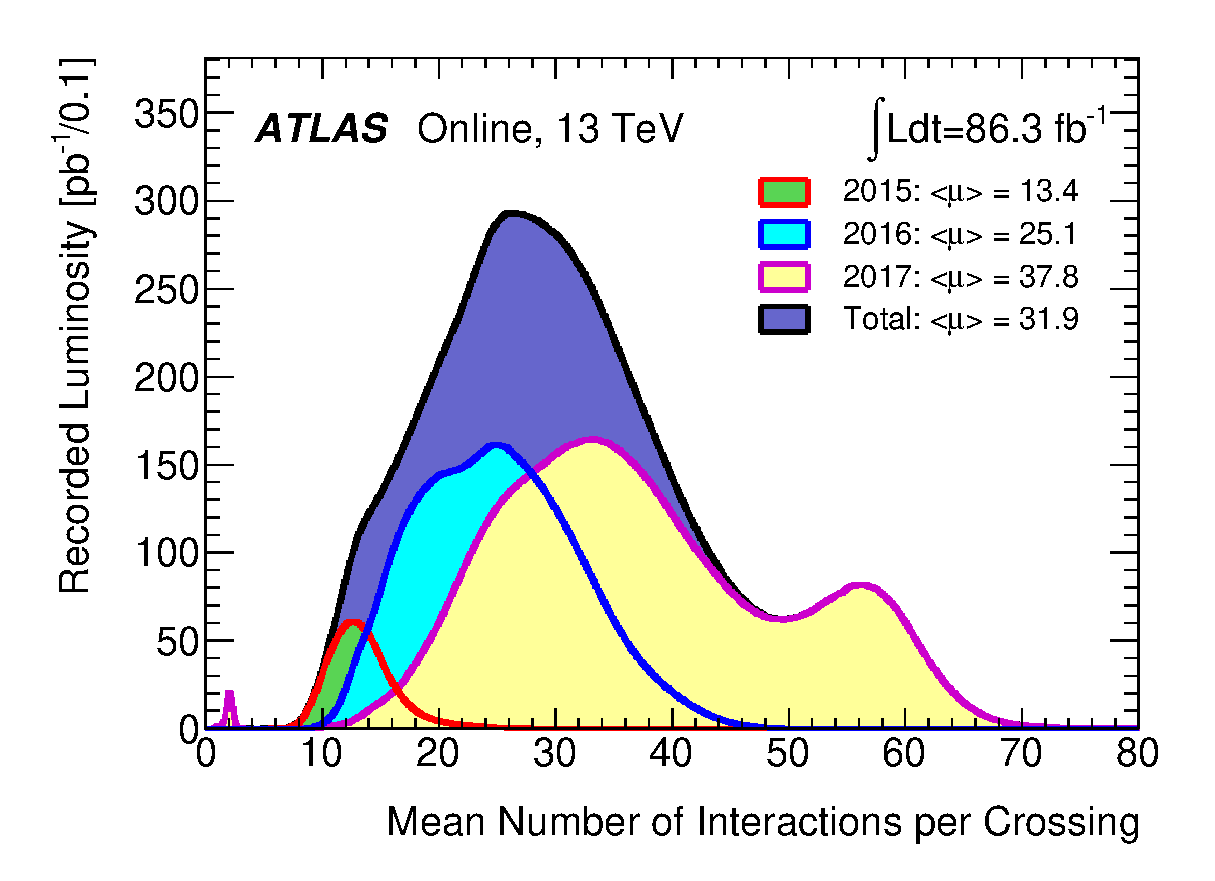
\includegraphics[width=\textwidth]{LHC/mu_2015_2017.eps}
 \caption[The luminosity-weighted distribution of the mean number of interactions per crossing for the 2015, 2016, and 2017 $pp$ collision data at $13~\TeV$ center-of-mass energy.]{%
  The luminosity-weighted distribution of the mean number of interactions per crossing for the 2015, 2016, and 2017 $pp$ collision data at $13~\TeV$ center-of-mass energy.
  All data recorded by ATLAS during stable beams is shown, and the integrated luminosity and the mean value, $\braket{\mu}$, are shown.
  The mean number of interactions per crossing corresponds to the mean of the Poisson distribution of the number of interactions per crossing calculated for each bunch.
  It is calculated from the instantaneous per bunch luminosity as $\mu = \luminosity_{\mathrm{bunch}} \times \sigma_{\mathrm{inel}} / f_{r}$ where $\luminosity_{\mathrm{bunch}}$ is the per bunch instantaneous luminosity, $\sigma_{\mathrm{inel}}$ is the inelastic cross section which is taken to be $80~\mathrm{mb}$ for $13~\TeV$ collisions, and $f_{r}$ is the LHC revolution frequency.
  The luminosity shown represents the preliminary $13~\TeV$ luminosity calibration released in February 2018, based on van-der-Meer beam-separation scans in 2017~\cite{ATLAS:pileup_2015_2017}.}
 \label{fig:mu_2015_2017}
\end{figure}


 \chapter{The ATLAS Experiment}\label{chapter:ATLAS}

\section{Overview}\label{sec:ATLAS_overview}

The ATLAS Experiment~\cite{PERF-2007-01} is one of the four main LHC experiments with the ATLAS detector, seen in \Cref{fig:ATLAS_detector}, located in the experiment cavern at Point 1 of the LHC roughly $100~\textrm{m}$ underground.
The ATLAS detector, henceforth also referred to as just ``ATLAS,'' is a general purpose, high luminosity particle physics detector designed to be able to search for as many types of interesting physics events as possible.
ATLAS is the largest of the LHC experiments with dimensions of $44~\mathrm{m}$ in length and $25~\mathrm{m}$ in height.

\begin{figure}[htbp]
 \centering
 \includegraphics[width=\textwidth]{ATLAS/ATLAS_detector.eps}
 \caption[Cut-away view of the ATLAS detector.]{%
  Model of human particle physicists with ATLAS detector shown for scale~\cite{Pequenao:1095924}.}\label{fig:ATLAS_detector}
\end{figure}

\clearpage
\section{Geometry}\label{sec:ATLAS_geometry}

The ATLAS detector is cylindrical in design and forward-backward symmetrical with respect to the center of the detector.
The inner detector is surrounded by a $2~\mathrm{T}$ superconducting solenoid magnet and provides excellent tracking coverage in $\abs{\eta} < 2.5$.
The inner detector is further bracketed at each end by end-cap toroid magnets and the entire barrel of the detector out through the calorimeters is enclosed in a toroid magnet system.
These two toroid systems are both constructed such that they exhibit an eight-fold azimuthal symmetry.
As a result, almost all of ATLAS also exhibits this eight-fold axial symmetry, with the noted exception of the support structures on the bottom that support the detector off the ground.
The detectors subsytems, described in the following sections, are radially concentric and cover different pseudorapidity ranges, with the liquid-argon (LAr) forward calorimeters extending the coverage out to $\abs{\eta} = 4.9$.

\section{Tracking in the Inner Detector}\label{sec:ATLAS_ID}

Located at the heart of ATLAS and inside of the $2~\mathrm{T}$ solenoidal magnetic field, the \gls{inner detector} subsystem, seen in \Cref{fig:ATLAS_inner_detector}, provides precision tracking through the combined performance of successive layers of pixel detectors, silicon \gls{SCT}, and the straw tube \gls{TRT} and provides excellent coverage up to $\abs{\eta} < 2.5$.
To maximize the effective detector area, the pixels and SCT in the barrel region are arranged in concentric cylinders, as seen in \Cref{fig:ATLAS_pixel}.
The pixel layers are closest to the beamline and consist of roughly $80.4$ million identical pixel sensors forming three cylindrical layers in the barrel and three consecutive disks at each end-cap.
Each of the pixels is of area\footnote{$50~\mu\mathrm{m}$ in the $R\textrm{-}\phi$ direction by $400~\mu\mathrm{m}$ in the $z$ direction.} $20,000~\mu\mathrm{m}^{2}$ with resolution of $10~\mu\mathrm{m}~(R\textrm{-}\phi) \times 115~\mu\mathrm{m}~(z)$.
This fine pixel cell size, and charge sharing between adjacent pixel cells --- given the reverse biased $p^{+}$-$n$ junction architecture --- give excellent spatial resolution in $R\textrm{-}\phi$ along with the strong magnetic field bending particles along $\hat{\vec{\phi}}$ causing them to spiral through the pixel detector~\cite{Aad:2008zz,PERF-2007-01}.
Charged particle hits in the pixel detector are paramount for robust tracking and identifying and reconstructing the primary and secondary vertices necessary for physics object reconstruction (i.e., jets) and flavor tagging.

\begin{figure}[htbp]
 \centering
 \includegraphics[width=0.65\textwidth]{ATLAS/ATLAS_inner_detector.eps}
 \caption[Cut-away view of the ATLAS inner detector showing the pixel detector, Semiconductor Tracker, and Transition Radiation Tracker.]{%
  Cut-away view of the ATLAS inner detector showing the pixel detector, Semiconductor Tracker, and Transition Radiation Tracker~\cite{Pequenao:1095926}.}\label{fig:ATLAS_inner_detector}
\end{figure}

\begin{figure}[htbp]
 \centering
 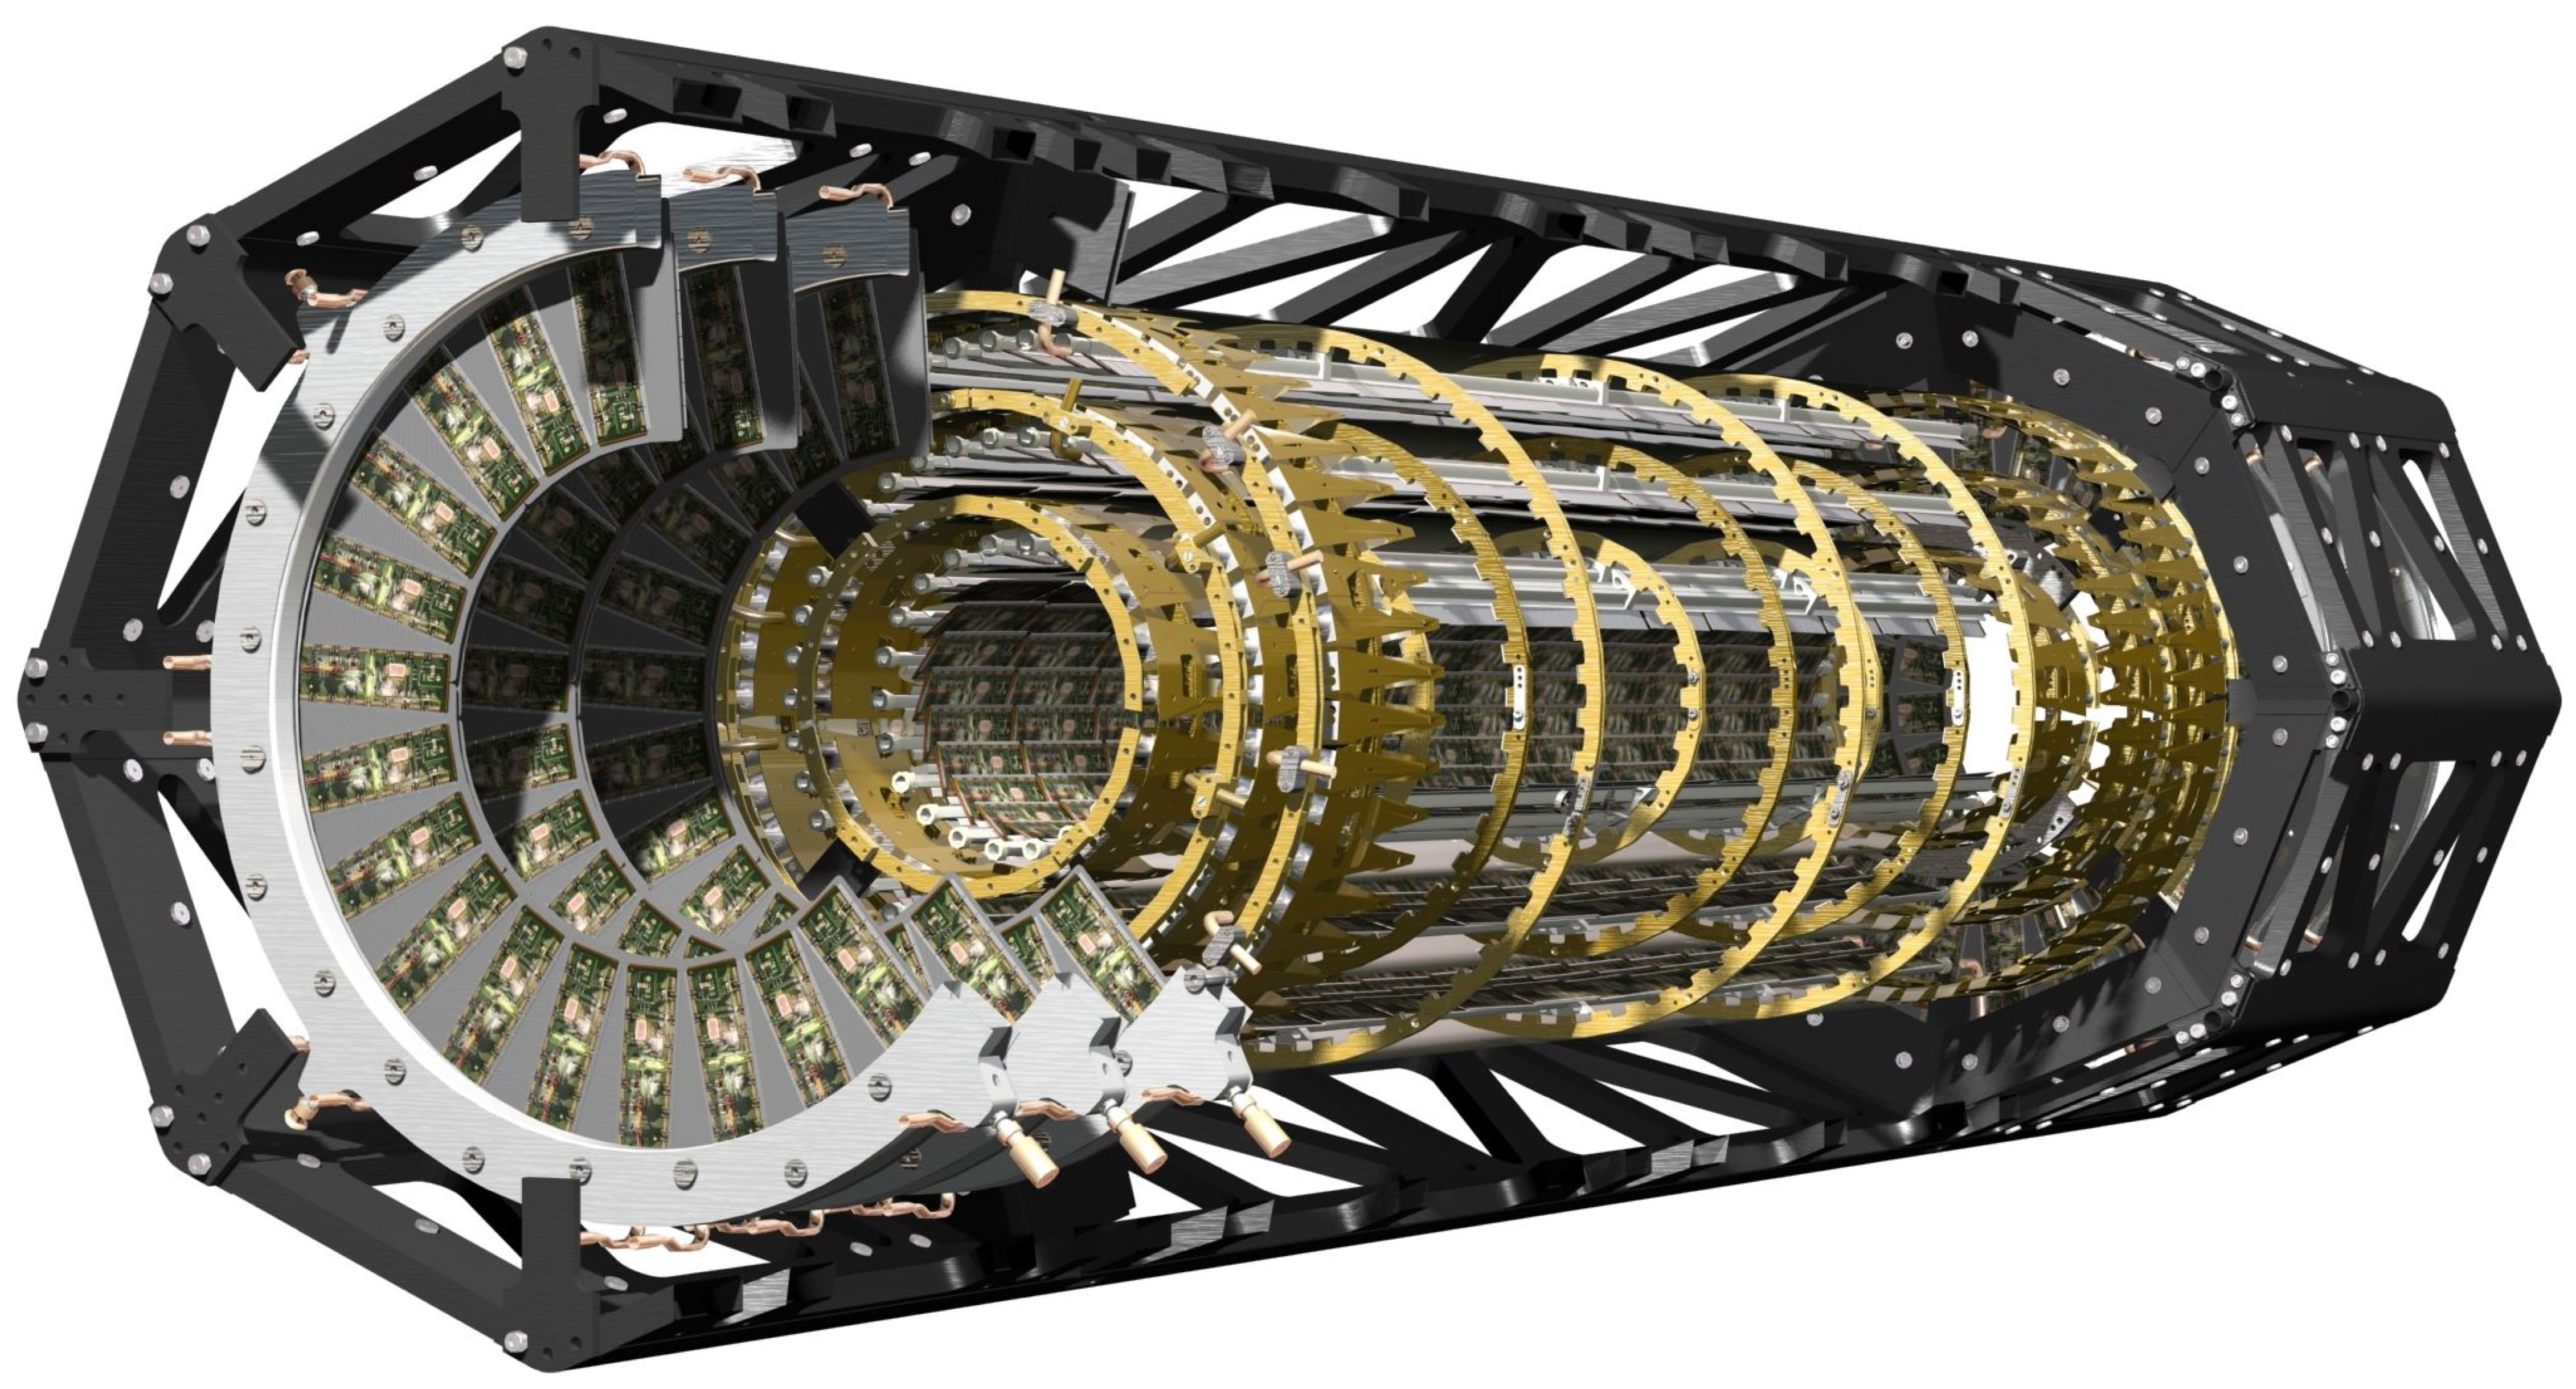
\includegraphics[width=0.6\textwidth]{ATLAS/ATLAS_pixel.eps}
 \caption[Cut-away view of the ATLAS pixel detector in the inner detector.]{%
  Cut-away view of the ATLAS pixel detector in the inner detector~\cite{Pequenao:1095925}.
  The pixel sensors form three cylindrical layers in the barrel and three consecutive disks at each end-cap.}\label{fig:ATLAS_pixel}
\end{figure}

The \Gls{SCT} surrounds the pixel detector in the barrel with four layers of stereo strips with small angle coverage $(40~\mathrm{mrad})$, shown in \Cref{fig:ATLAS_inner_detector_radial_view}, to measure hits in the silicon in both $R\textrm{-}\phi$ and $z$.
In the end-cap region, the SCT strips run radially in nine disks in each end-cap (for 18 disk in total).
In total, the SCT has roughly 6.3 million readout channels and results in track resolutions of $17~\mu\mathrm{m}~(R\textrm{-}\phi) \times 580~\mu\mathrm{m}~(z)$ in the barrel region and $17~\mu\mathrm{m}~(R\textrm{-}\phi) \times 580~\mu\mathrm{m}~(R)$ in the end-cap region.

The \Gls{TRT} further extends the ID $R\textrm{-}\phi$ information up to $\abs{\eta} = 2.0$ by providing a large number of track interactions with its approximately $351,000$ $4~\textrm{mm}$ straw tubes.
In the barrel region, the TRT straw tubes are parallel to the beam axis, shown in \Cref{fig:ATLAS_inner_detector_radial_view}, and extend for $144~\mathrm{cm}$ on either side of $\eta = 0$.
In the end-cap region, $37~\mathrm{cm}$ TRT straws are radially arranged with respect to the beamline in wheels, shown in \Cref{fig:ATLAS_inner_detector}.
Combined with the precision tracking from the pixel detectors and SCT, the tracking information that the TRT gives at larger radii contributes to high precision tracking of charged particles in both $R\textrm{-}\phi$ and $z$, and the large number of hits in the TRT significantly improve momentum measurements.

\begin{figure}[htbp]
 \centering
 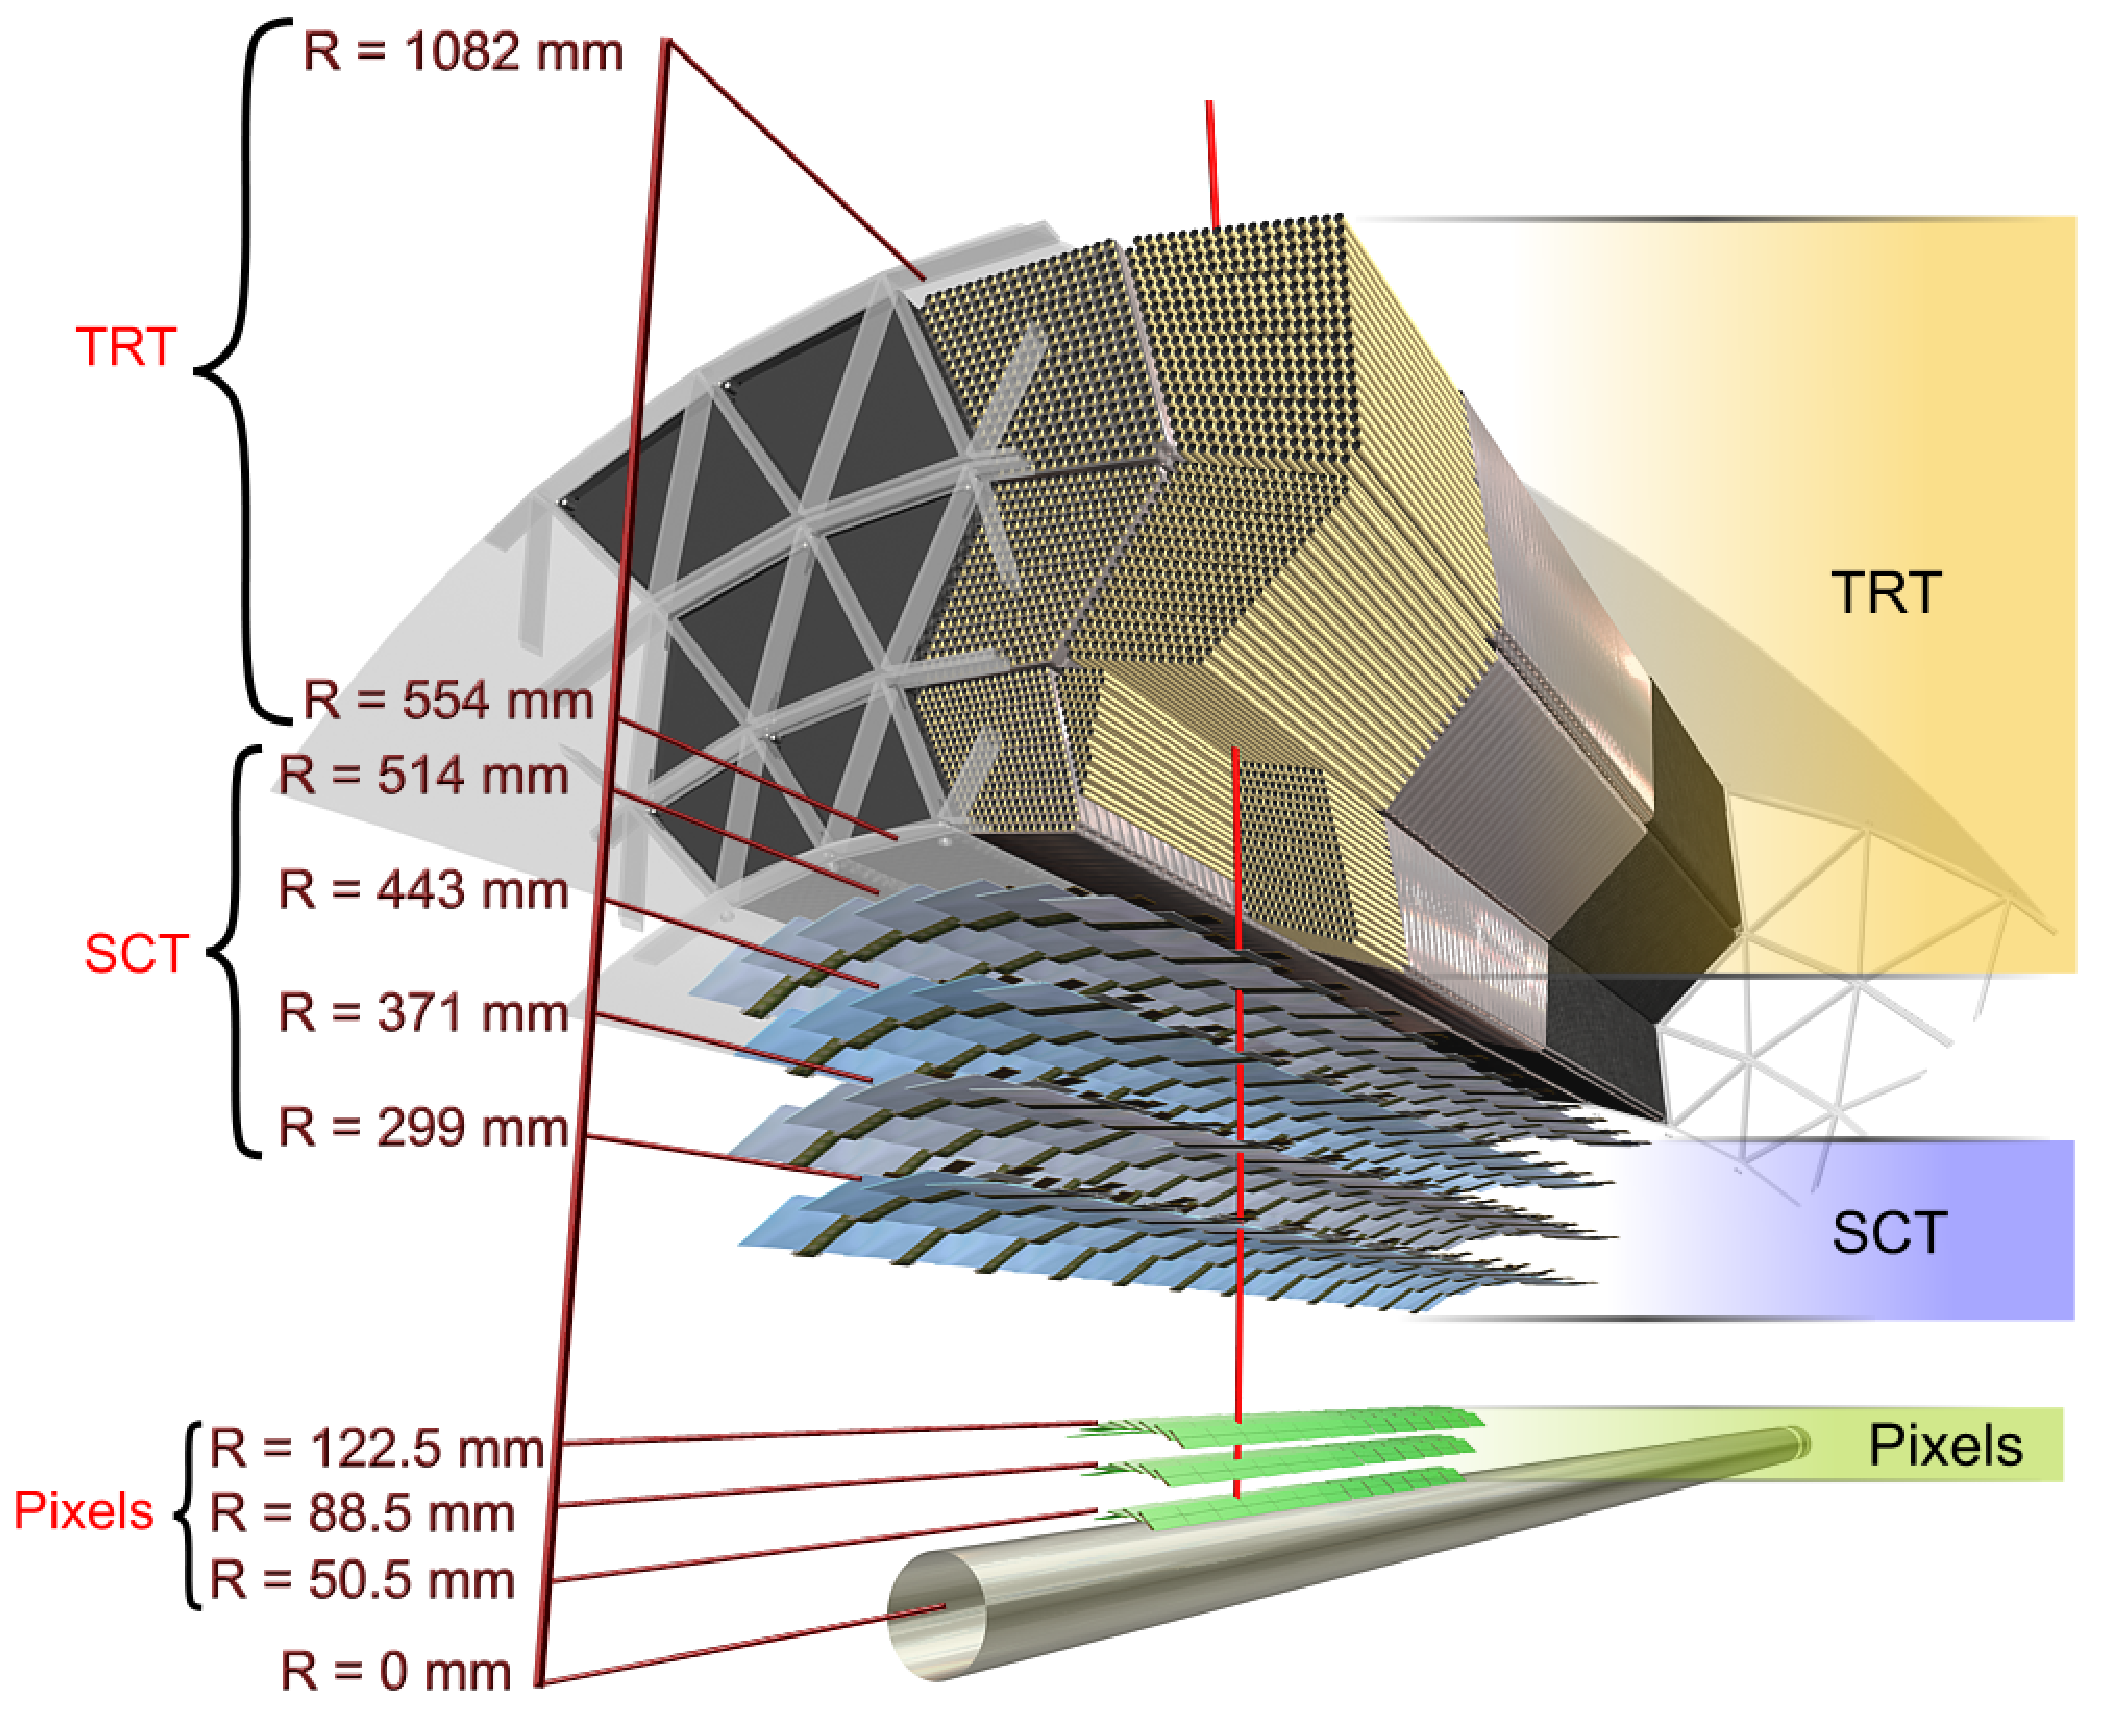
\includegraphics[width=0.6\textwidth]{ATLAS/ATLAS_inner_detector_radial_view.eps}
 \caption[Scale cut-away view of the pixel detector, Semiconductor Tracker, and Transition Radiation Tracker in the barrel-region.]{%
  The sensors and structural elements traversed by a charged track of $10~\GeV$ $p_{T}$ in the barrel inner detector $(\abs{\eta} = 0.3)$.
  The track traverses successively the beryllium beam-pipe, the three cylindrical silicon-pixel layers with individual sensor elements of $50 \times 400~\mu\mathrm{m}^{2}$, the four cylindrical double layers (one axial and one with a stereo angle of $40~\mathrm{mrad}$) of barrel SCT sensors of pitch $80~\mu\mathrm{m}$, and approximately 36 axial straws of $4~\mathrm{mm}$ diameter contained in the barrel TRT modules within their support structure~\cite{PERF-2007-01}.}\label{fig:ATLAS_inner_detector_radial_view}
\end{figure}

\clearpage
\section{Calorimeter System}\label{sec:ATLAS_calo}

The ATLAS calorimeter system, shown in \Cref{fig:ATLAS_calorimeter}, provides excellent energy deposition measurements for particles with coverage up to $\abs{\eta} < 4.9$ with different calorimetry subsystems for various physics processes.
In the pseudorapidity range of the inner detector ($\abs{\eta} < 2.5$) the high granularity electromagnetic (EM) liquid argon calorimeter system provides measurement of electrons and photons.
The more coarse resolution of the hadronic calorimeter systems provides measurements for jet reconstruction and missing transverse momentum, $\MET$, in conjunction with the large pseudorapidity coverage.
These calorimeter designs are both ``sampling calorimeters,'' where the ``active'' materials that provide the signals are different from the ``absorber'' materials that reduce the particle energy and cause showering.
The calorimeter subsystems are also designed to be sufficiently thick as to contain the electromagnetic and hadronic showers that originate inside them, and to limit punch-through to the muon systems.

\begin{figure}[htbp]
 \centering
 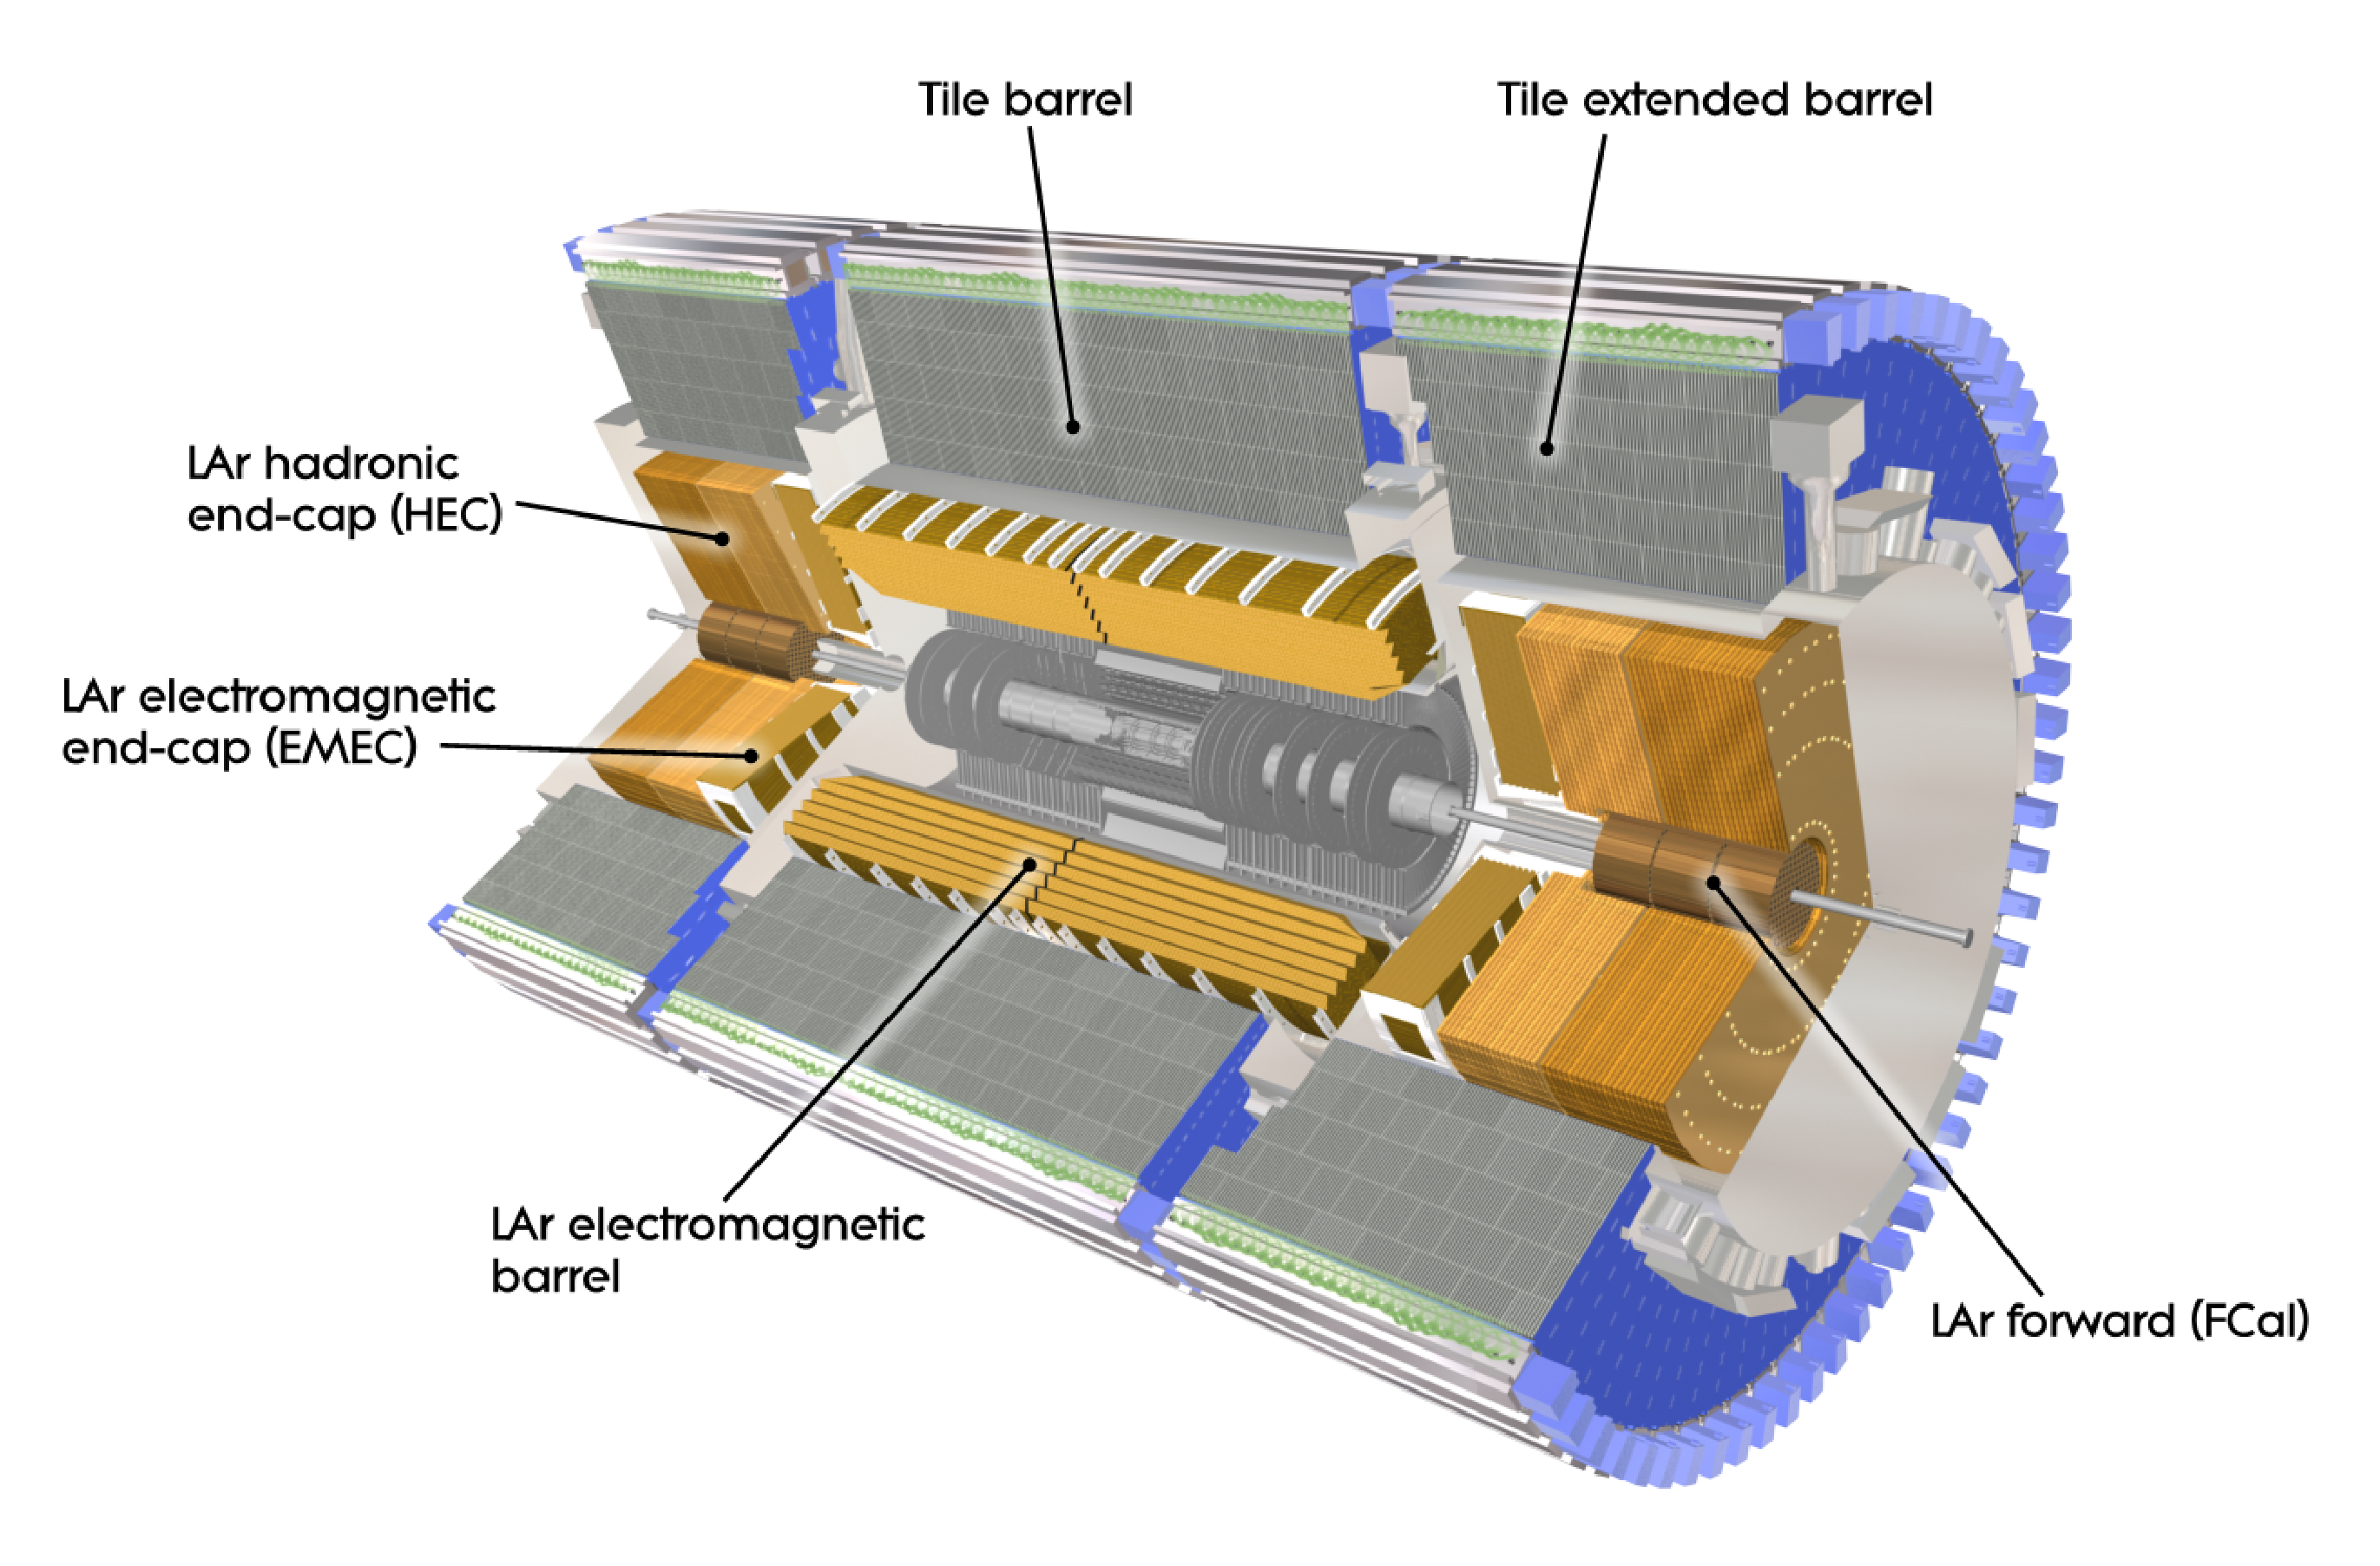
\includegraphics[width=0.8\textwidth]{ATLAS/ATLAS_calorimeter.eps}
 \caption[Cut-away view of the ATLAS calorimeter system.]{%
  Cut-away view of the ATLAS calorimeter system~\cite{Pequenao:1095927}.}\label{fig:ATLAS_calorimeter}
\end{figure}

\clearpage
\subsection{Electromagnetic Calorimeter}\label{sec:ATLAS_electromagnetic_calorimeter}

The electromagnetic calorimeter system, shown in \Cref{fig:ATLAS_LAr}, consists of lead-liquid argon detectors with a characteristically unique ``accordion'' lead absorber plate design that allows for continuous coverage in $\phi$ with folding angles of the accordion ``waves'' that vary with the radius to keep the LAr gap constant, as shown in \Cref{fig:ATLAS_LAr_module}.
Liquid argon (LAr) is the active detector material for the EM calorimeters as it has a linear behavior, very stable response over time, and is intrinsically radiation-hard.
In the barrel region the LAr EM calorimeter is split into symmetric half-barrels, and in the end-caps the LAr EM calorimeter exists as two coaxial wheels, respectively covering the regions of $1.375 < \abs{\eta} < 2.5$ and $2.5 < \abs{\eta} < 3.2$.

\begin{figure}[htbp]
 \centering
 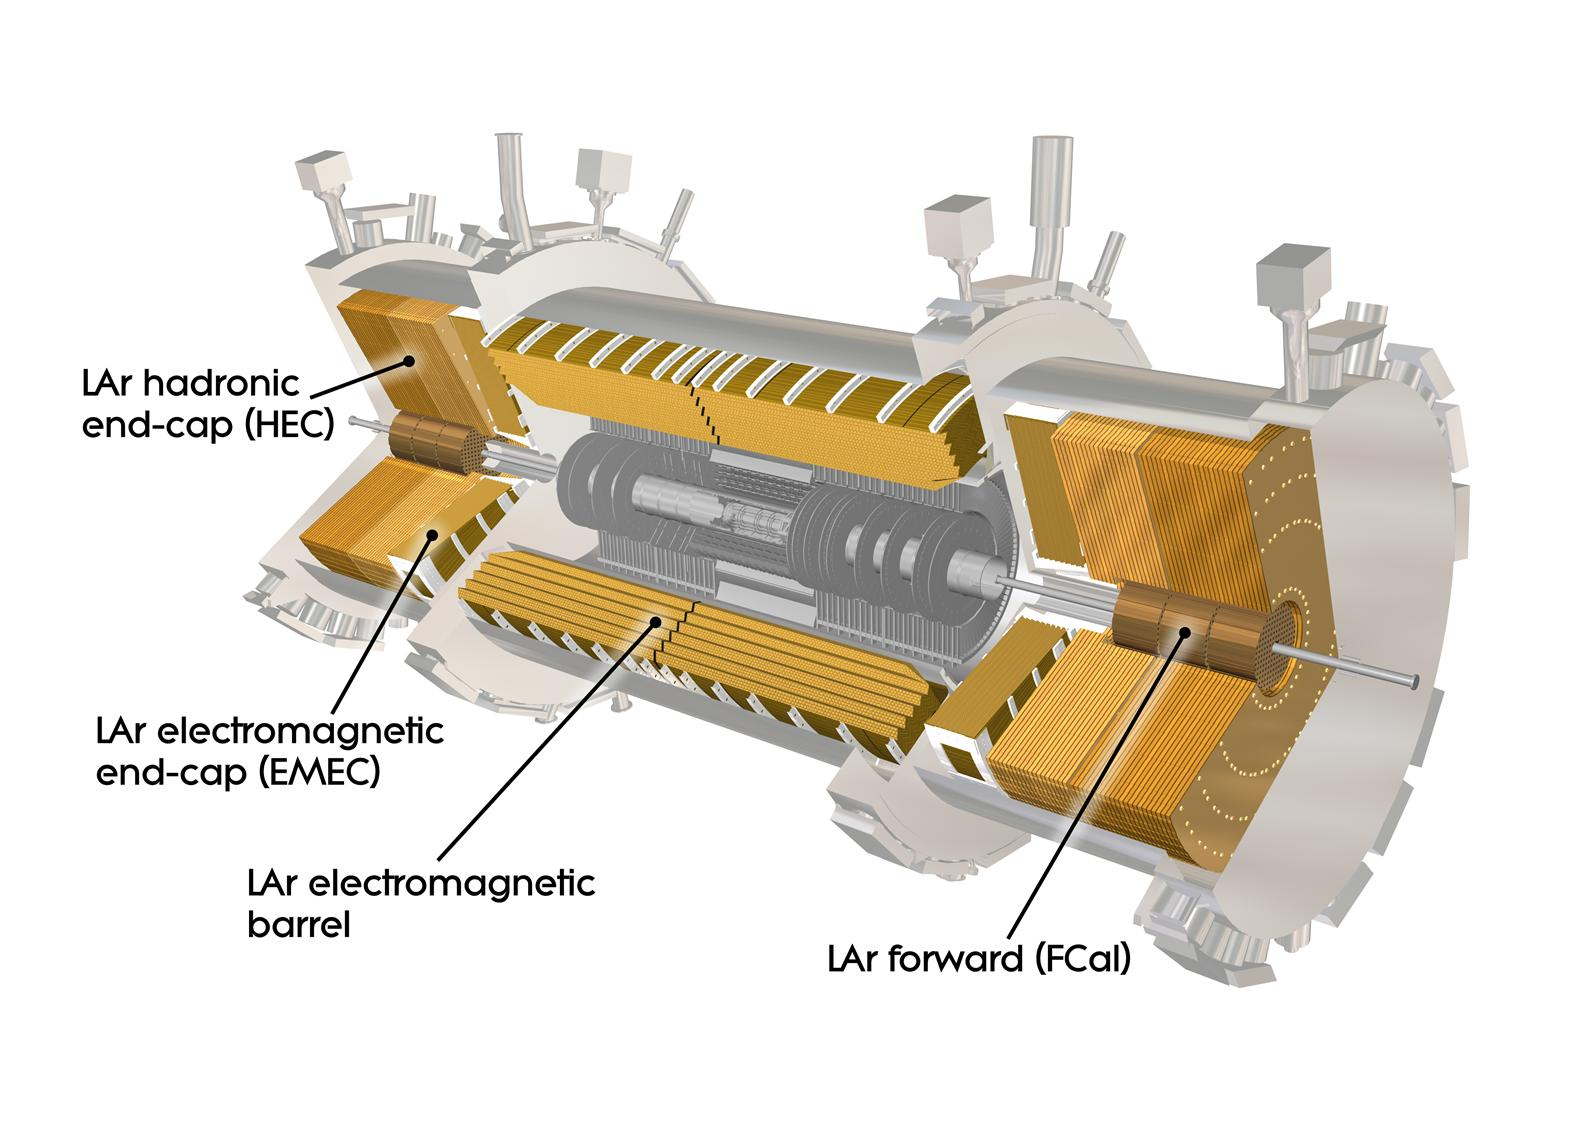
\includegraphics[width=0.7\textwidth]{ATLAS/ATLAS_LAr.jpg}
 \caption[Cut-away view of the ATLAS electromagnetic liquid argon calorimeter system.]{%
  Cut-away view of the ATLAS electromagnetic liquid argon calorimeter system~\cite{Pequenao:1095927}.}\label{fig:ATLAS_LAr}
\end{figure}

\begin{figure}[htbp]
 \centering
 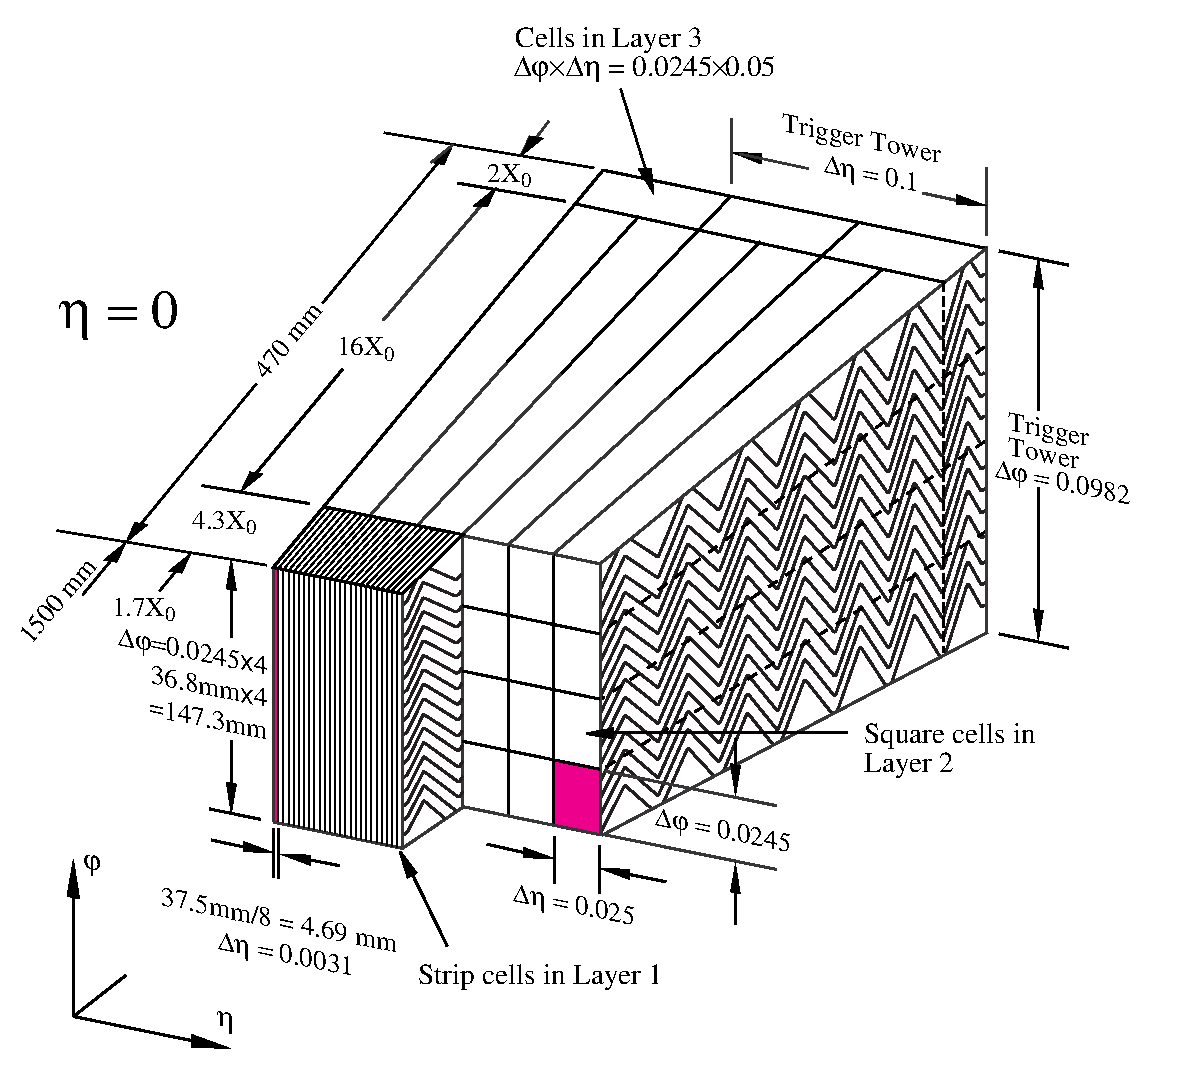
\includegraphics[width=0.6\textwidth]{ATLAS/ATLAS_LAr_module.eps}
 \caption[Sketch of a liquid argon calorimeter system barrel module detailing granularity in $\eta$ and $\phi$.]{%
  Sketch of a barrel module where the different layers are clearly visible with the ganging of electrodes in $\phi$.
  The granularity in $\eta$ and $\phi$ of the cells of each of the three layers and of the trigger towers is also shown~\cite{PERF-2007-01}.}\label{fig:ATLAS_LAr_module}
\end{figure}

\subsection{Hadronic Calorimeter}\label{sec:ATLAS_hadronic_calorimeter}

The hadronic calorimeter system is composed of the tile calorimeters in the barrel region, and the LAr Hadronic End-cap Calorimeter (HEC) and LAr Forward Calorimeter (FCal) in the end-cap region.
The tile sampling calorimeter resides outside the EM calorimeter system and provides coverage out to $\abs{\eta} < 1.7$ and radial coverage from $2.28~\mathrm{m}$ out to $4.25~\mathrm{m}$.
The tile calorimeter absorber material is steel and uses scintillating tiles as the active material, which are read out using wavelength shifting fibers into photomultiplier tubes.
The HEC exists as two wheels in each end-cap behind the end-cap EM calorimeter, extending the coverage in the end-caps out to $\abs{\eta} < 3.2$.
The copper absorber plates of the HEC are interleaved with $8.5~\mathrm{mm}$ spacers of LAr providing active material.
The FCal extends coverage from $3.1 < \abs{\eta} < 4.9$ and is composed of three modules in each end-cap: a copper module optimized for electromagnetic measurements, and then two made of tungsten for hadronic interaction measurements.
The modules are a metal matrix with regularly spaced longitudinal channels consisting of tubes with a concentric rod and LAr filling the gap between them.

For calorimetry systems the energy resolution improves as the energy of the particle, $E$ increases, generally as $1/\sqrt{E}$.
More specifically, the energy resolution, $\sigma\left(E\right)$, of a calorimeter is given as the quadrature sum%
\footnote{That is, $a \oplus b = \sqrt{a^{2} + b^{2}}$.}
\begin{equation}
 \frac{\sigma\left(E\right)}{E} = \frac{a}{\sqrt{E}} \oplus \frac{b}{E} \oplus c\,,
 \label{eq:calorimeter_energy_resolution}
\end{equation}
where $a$ is the ``stochastic term'' for intrinsic shower fluctuations, $b$ is the ``noise term,'' and $c$ is the ``constant'' term~\cite{Fabjan:692252}.
It is seen from \Cref{eq:calorimeter_energy_resolution} that at lower energies the stochastic term is more important and at higher energies the constant term affects the energy resolution more.
The ATLAS calorimeters are designed to have excellent energy resolution, which is clearly seen from the observed energy resolution for the ATLAS LAr EM calorimeter barrel region in testbeam experiments~\cite{Ilic:2014,Aleksa:1547314}
\[
 \frac{\sigma\left(E\right)}{E} = \frac{10\%}{\sqrt{E}} \oplus \frac{200~\MeV}{E} \oplus 0.2\%\,.
\]
For the hadronic calorimeters the stochastic term is required to be under $50\%$ and the constant term under $3\%$~\cite{Ilic:2014}.

\section{Muon Spectrometer}\label{sec:ATLAS_muon_spectrometer}

The ATLAS \gls{muon spectrometer}, shown in \Cref{fig:ATLAS_muon_spectrometer}, is arranged as the exterior detector subsystem to provide coverage for muons deflected from the air-core toroid magnets.
As muons are minimum ionizing particles%
\footnote{The mass stopping power for muons in the typical energy ranges at the LHC is less than $4~\MeV\,\mathrm{cm}^{2}/\mathrm{g}$.
 To put this in context, a $1~\GeV$ muon can punch through roughly $1~\mathrm{m}$ of iron before stopping~\cite{Garutti:lecture}.}
, as seen in \Cref{fig:Bethe-Bloch_stopping_power}, they pass through the inner detector and calorimeter systems while being radially deflected by the solenoid magnetic field before entering the toroidal magnetic field and getting deflected along $\hat{\vec{z}}$.
Given the resulting trajectories, in the barrel region muon tracks are measured by three cylindrical layers of \glspl{MDT}, shown in \Cref{fig:ATLAS_MDT_chamber} and \Cref{fig:ATLAS_muon_barrel_track}, and in the end-caps region three planes of MDT wheels before escaping the detector altogether --- hence the name \emph{spectrometer}.
For most of the $\eta$ range the MDTs perform most of the precision measurements of the tracks, though from $2 < \abs{\eta} < 2.7$ higher granularity \glspl{CSC} provide tracking to withstand the intense rate and radiation~\cite{PERF-2007-01}.

\begin{figure}[htbp]
 \centering
 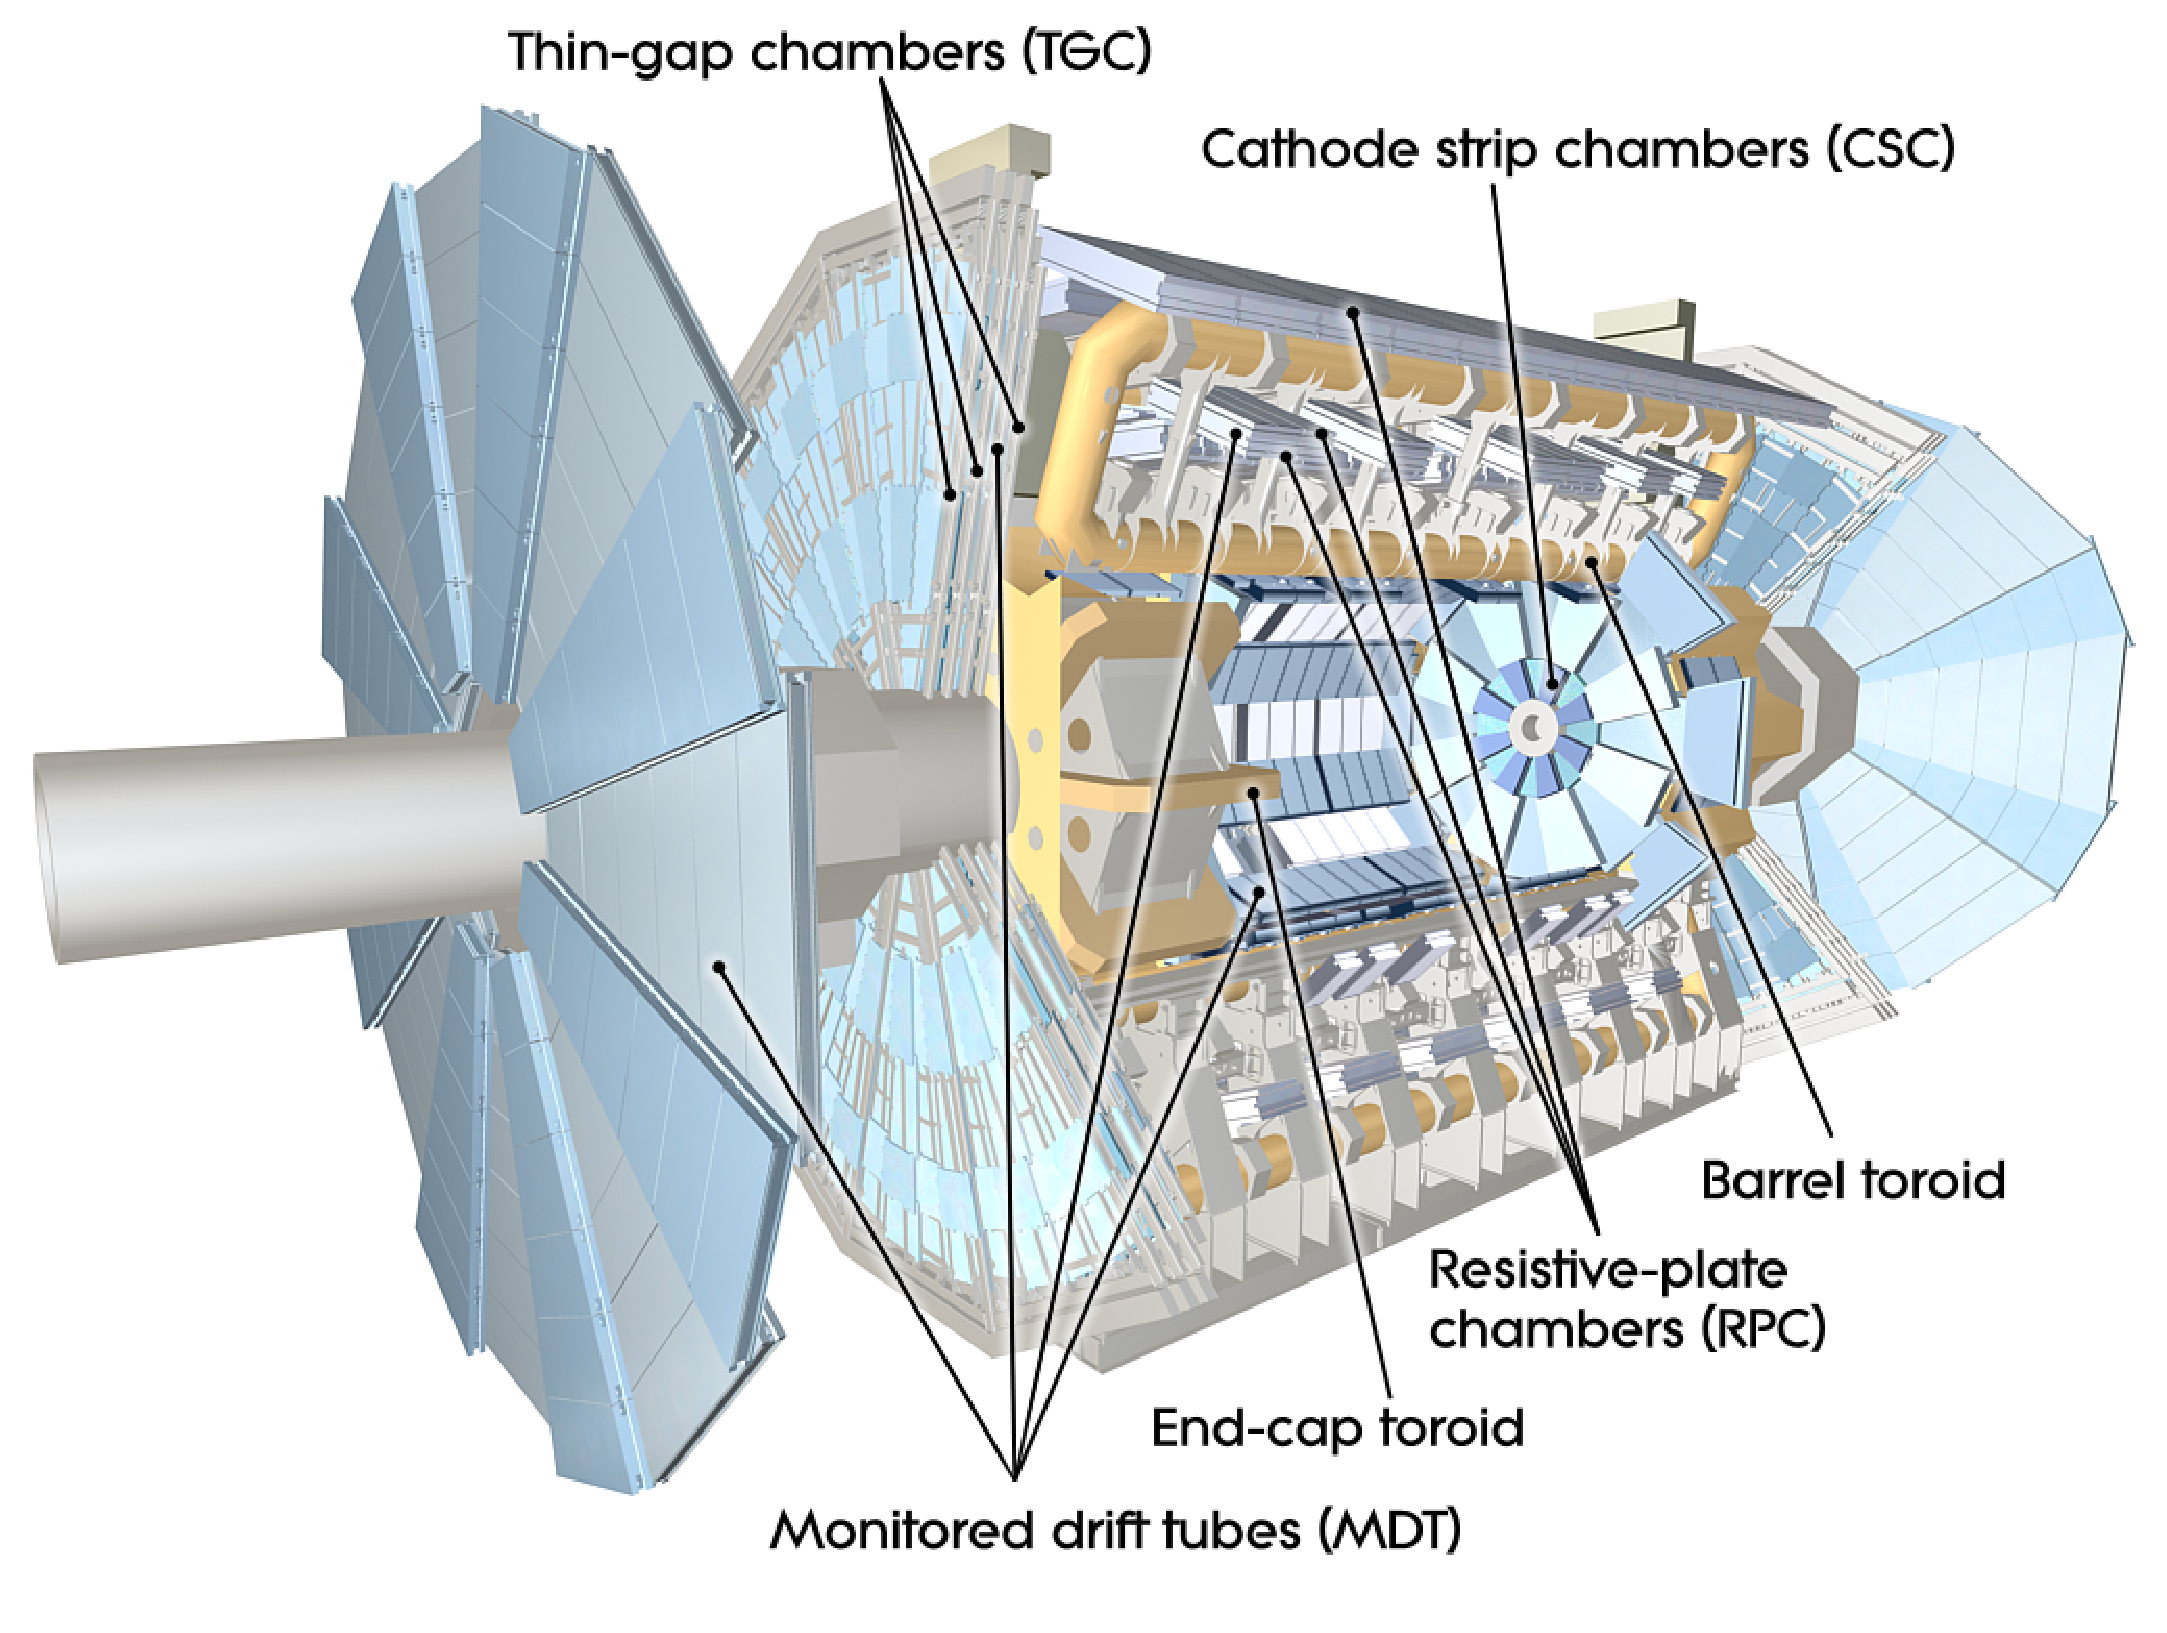
\includegraphics[width=0.6\textwidth]{ATLAS/ATLAS_muon_spectrometer.eps}
 \caption[Cut-away view of the ATLAS muon system.]{%
  Cut-away view of the ATLAS muon system~\cite{PERF-2007-01}.}\label{fig:ATLAS_muon_spectrometer}
\end{figure}

\begin{figure}[htbp]
 \centering
 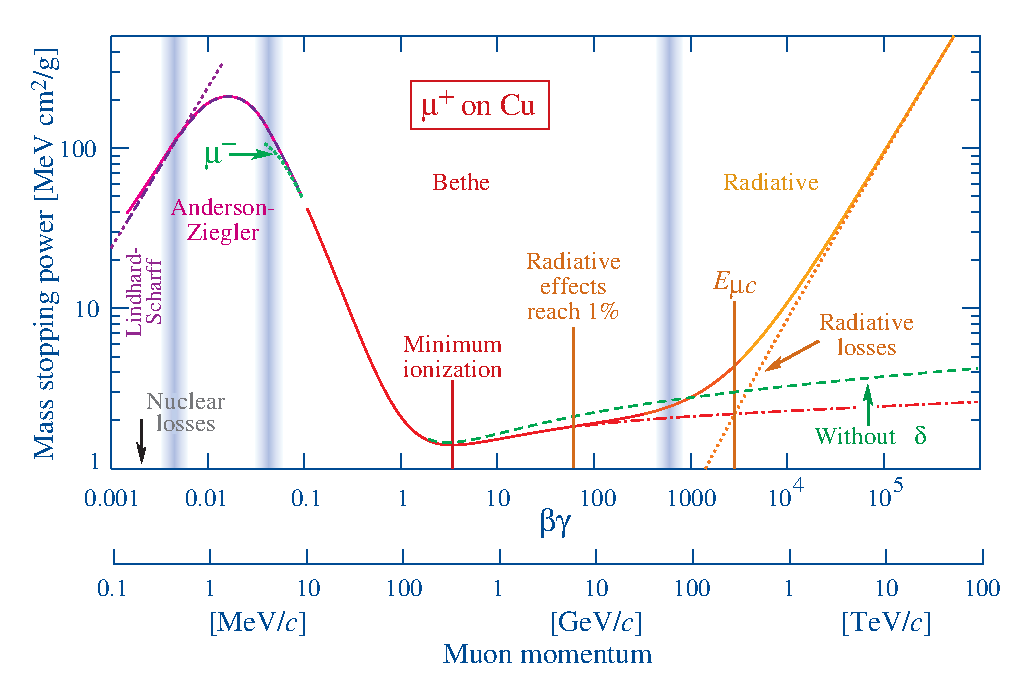
\includegraphics[width=\textwidth]{ATLAS/Bethe-Bloch_stopping_power.eps}
 \caption[Mass stopping power for positive muons in copper as a function of $\beta \gamma = p/Mc$.]{%
  Mass stopping power $\left(= \left<-dE/dx\right>\right)$ for positive muons in copper as a function of $\beta \gamma = p/Mc$ over nine orders of magnitude in momentum (12 orders of magnitude in kinetic energy).
  Solid curves indicate the total stopping power.
  Data below the break at $\beta \gamma \approx 0.1$ are taken from ICRU 49~\cite{ICRU49}, and data at higher energies are from~\cite{Groom:2001kq}.
  Vertical bands indicate boundaries between different approximations discussed in~\cite{PDG2018:Ch33}.
  The short dotted lines labeled ``$\mu^{-}$'' illustrate the ``Barkas effect,'' the dependence of stopping power on projectile charge at very low energies~\cite{PhysRev.101.778}.
  $dE/dx$ in the radiative region is not simply a function of $\beta$~\cite{PDG2018:Ch33}.}\label{fig:Bethe-Bloch_stopping_power}
\end{figure}

\begin{figure}[htbp]
 \centering
 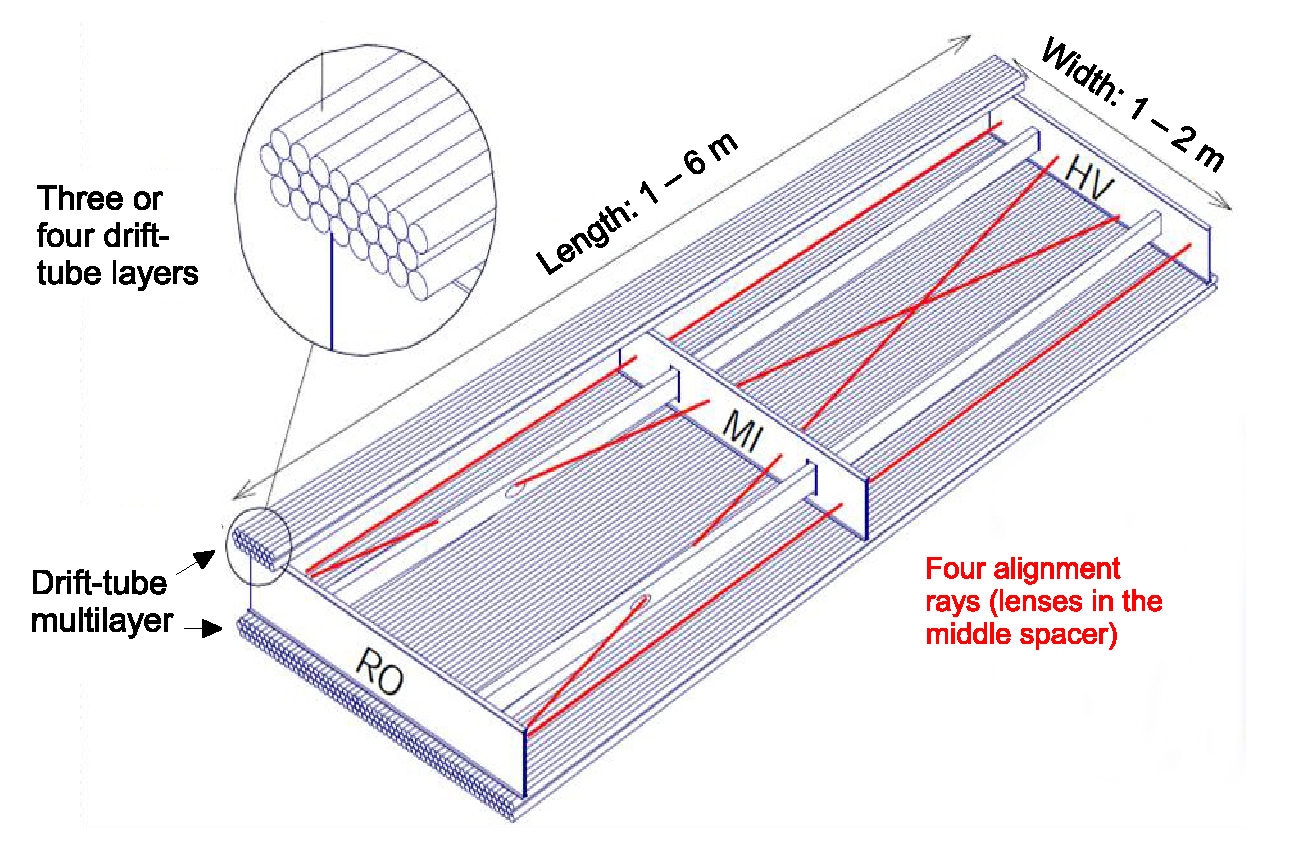
\includegraphics[width=0.6\textwidth]{ATLAS/ATLAS_MDT_chamber.eps}
 \caption[Mechanical structure of a monitored drift tube chamber.]{%
  Mechanical structure of a \gls{MDT} chamber.
  Three spacer bars connected by longitudinal beams form an aluminium space frame, carrying two multi-layers of three or four drift tube layers.
  Four optical alignment rays, two parallel and two diagonal, allow for monitoring of the internal geometry of the chamber.
  RO and HV designate the location of the readout electronics and high voltage supplies, respectively~\cite{PERF-2007-01}.}\label{fig:ATLAS_MDT_chamber}
\end{figure}

\begin{figure}[htbp]
 \centering
 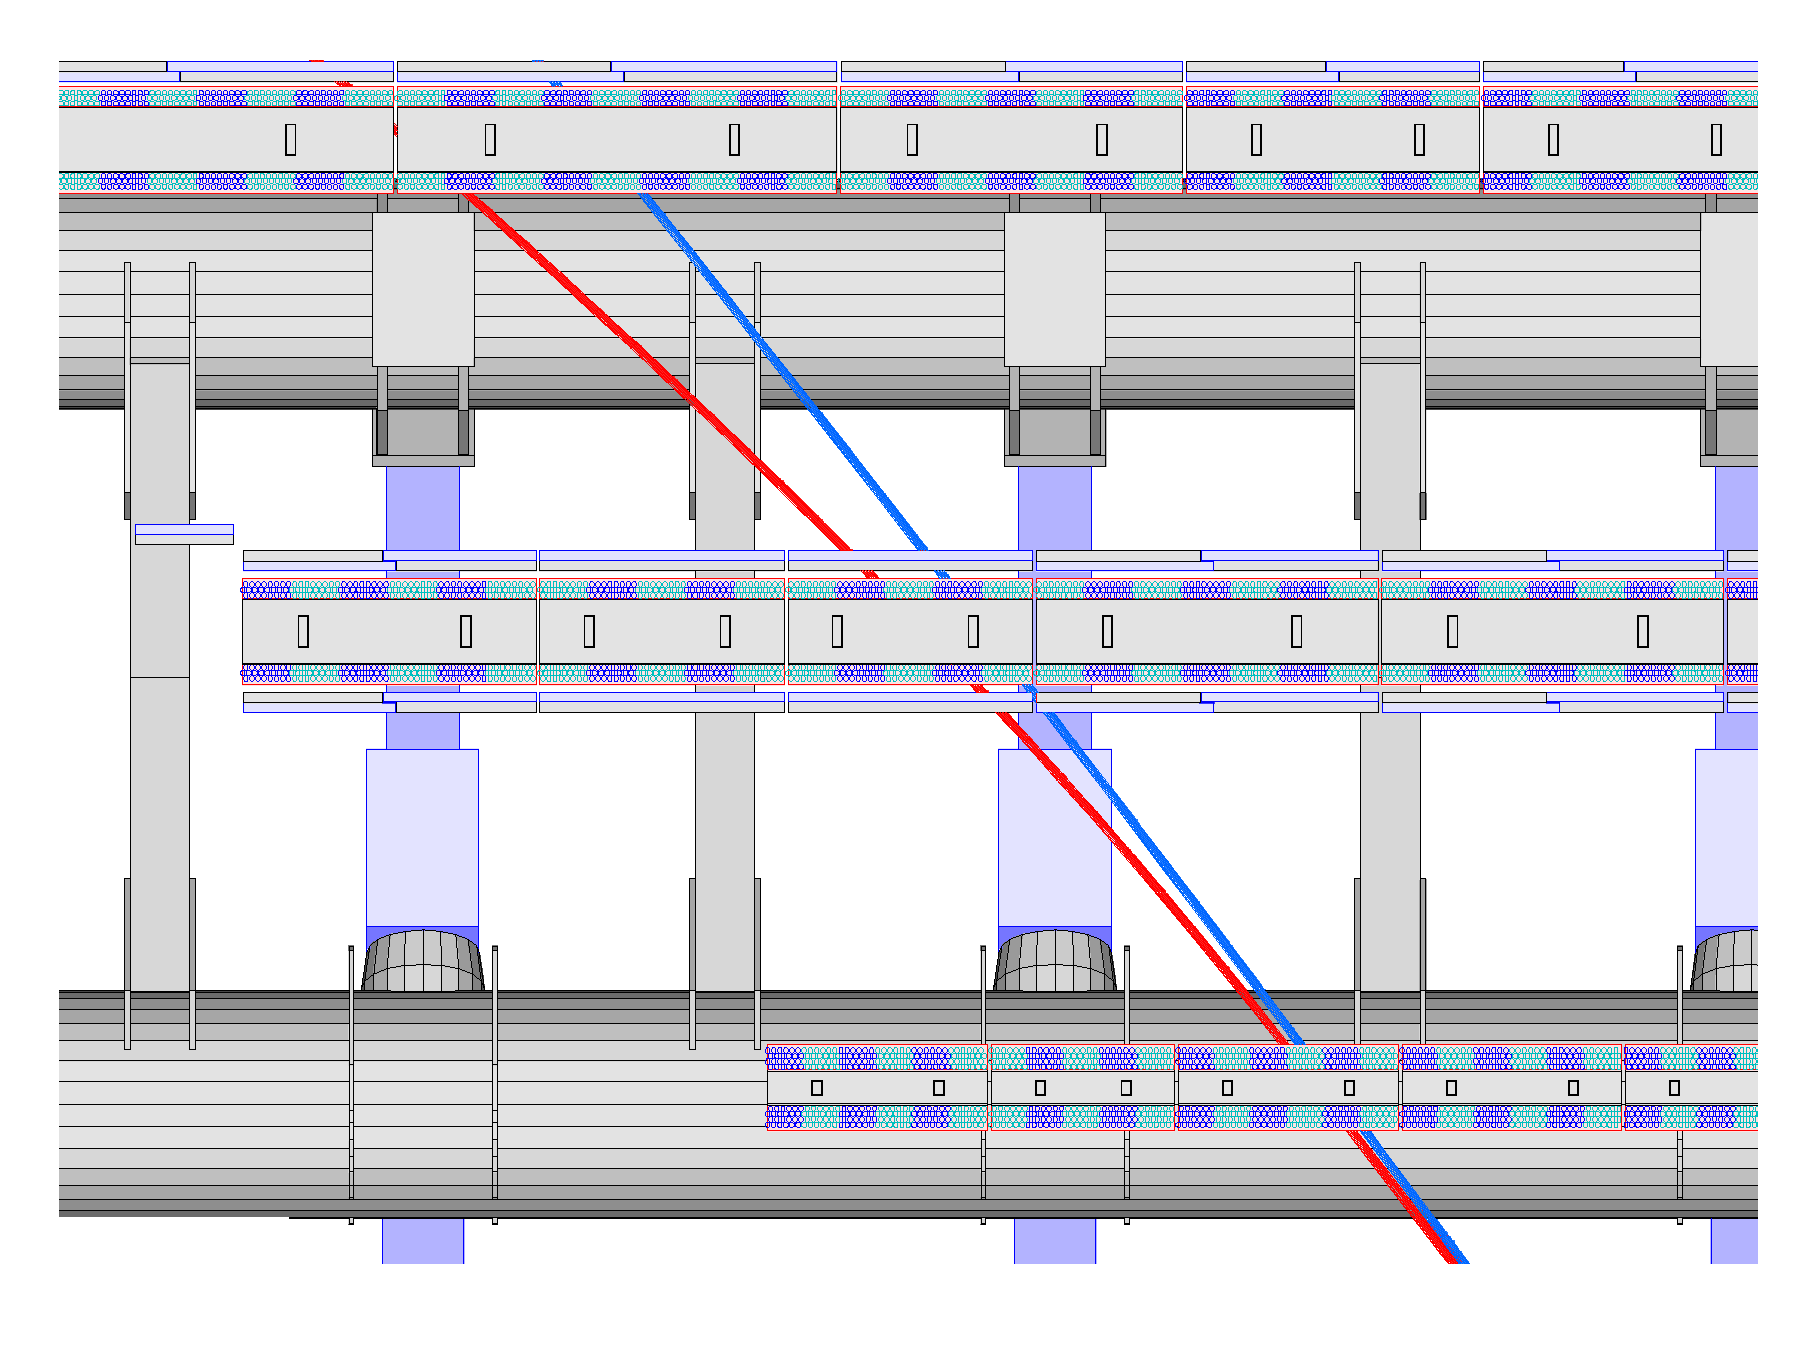
\includegraphics[width=0.6\textwidth]{ATLAS/ATLAS_muon_barrel_track.eps}
 \caption[Trajectories of muons through the three layers of monitored drift tube of the barrel muon spectrometer.]{%
  Trajectories of muons with momenta of $4~\GeV$ and $20~\GeV$ in the bending plane of the barrel muon spectrometer.
  In general, the tracks cross $2 \times 4$ inner, $2 \times 3$ middle, and $2 \times 3$ outer layers of \gls{MDT} tubes.
  The cyan and dark blue areas in each MDT layer illustrate the granularity of the mezzanine cards~\cite{PERF-2007-01}.}\label{fig:ATLAS_muon_barrel_track}
\end{figure}

The trigger system for the muon system provides coverage out to $\abs{\eta} < 2.4$ and the \gls{RPC} and \gls{TGC} trigger chambers uniquely provide bunch-crossing identification, well-defined $p_{T}$ thresholds, and measurements of the muon track coordinate in the orthogonal direction of the precision-tracking chambers~\cite{PERF-2007-01}.

\section{Trigger and Data Acquisition}\label{sec:ATLAS_TDAQ}

The ATLAS \gls{TDAQ} systems, shown in \Cref{fig:ATLAS_TDAQ_system}, function collectively at two different levels: the L1 trigger and the \gls{HLT}.
Collectively, the trigger system is responsible for reducing the approximately $1~\mathrm{GHz}$ event rate from the $25~\mathrm{ns}$ bunch crossings%
\footnote{Often reported as the equivalent $40~\mathrm{MHz}$ bunch crossing rate.}
--- which is not possible to write out and save in real time --- to a much more manageable $1~\mathrm{kHz}$ that can be written to storage~\cite{TRIG-2016-01}.
With raw event sizes of approximately $1.6~\mathrm{Mbytes}$ this still results in data generation of over a Gigabyte per second.

\begin{figure}[htbp]
 \centering
 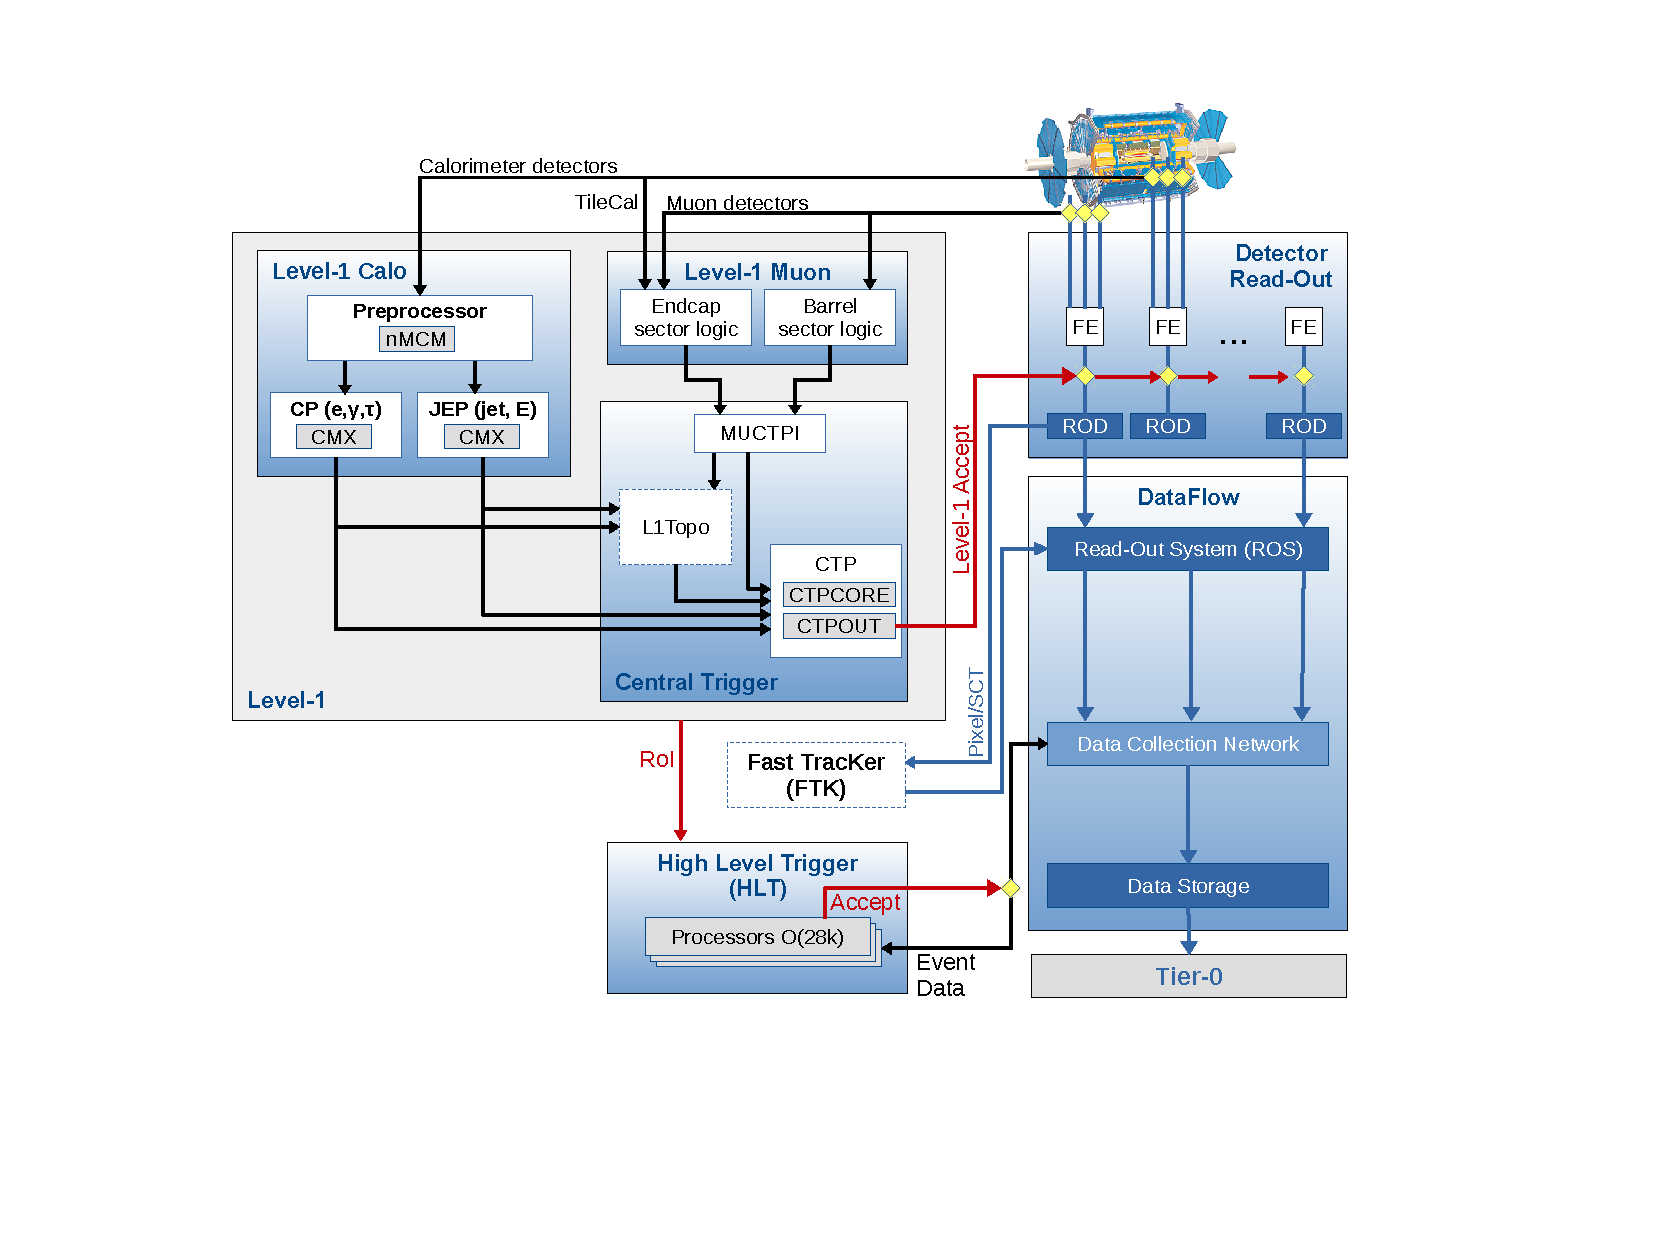
\includegraphics[width=\textwidth]{ATLAS/ATLAS_TDAQ_system.pdf}
 \caption[The ATLAS Trigger and Data Acquisition system in Run 2 with emphasis on the components relevant for triggering.]{%
  The ATLAS \gls{TDAQ} system in Run 2 with emphasis on the components relevant for triggering.
  L1Topo was installed in 2016 and commissioned during Run 2 and FTK is an upgrade for Run 3~\cite{TRIG-2016-01}.}\label{fig:ATLAS_TDAQ_system}
\end{figure}

\subsection{Level-1 Trigger (L1)}\label{sec:ATLAS_L1_trigger}

The Level-1 trigger (L1) is a hardware trigger system responsible for taking data coming from the ATLAS calorimeter and muon systems and identifying \gls{RoI}, shown in \Cref{fig:ATLAS_L1Calo_trigger_tower}, for cluster trigger candidates and further decision making within $2.5~\mu\mathrm{s}$ after the bunch-crossing associated with the event~\cite{PERF-2007-01}.
The L1Calo trigger algorithms search for high transverse momentum electrons, photons, jets, hadronically decaying $\tau$-leptons, and large $\MET$ signatures.
It does this by identifying RoIs in a sliding $4 \times 4$ window of trigger tower clusters in the calorimeters and using information from six elements formed from the sum of transverse energy in trigger tower groups~\cite{Eisenhandler:792528}:
\begin{enumerate}
 \item Four trigger tower regions (the sums shown in \Cref{fig:ATLAS_L1Calo_trigger_tower}) that measure the $\ET$ of EM showers.
 \item A hadronic core (the red box in \Cref{fig:ATLAS_L1Calo_trigger_tower}) from the four hadronic towers centered behind the EM clusters whose sum is used for isolation in the hadronic calorimeter.
 \item Four hadronic clusters summed over the EM and hadronic calorimeters that measure the $\ET$ of hadronic showers.
 \item An EM isolation ring formed from the twelve EM towers surrounding the EM core whose sum is used for isolation checks in the EM calorimeter.
 \item A hadronic isolation ring formed from the twelve hadronic towers behind the EM isolation ring whose sum is used for isolation checks in the hadronic calorimeter.
 \item A $2 \times 2 $ tower cluster RoI centered in the algorithm window and summed over the EM cluster region and hadronic core used to identify candidate RoIs.
\end{enumerate}

From these six elements algorithms then make decisions on the order of nanoseconds to classify the window as containing an EM cluster trigger candidate or a hadronic cluster trigger candidate\footnote{It is worth reflecting here that given the stringent requirements that the L1 trigger must meet that the fantastically complex objects that are hadronic jets start off as a L1 trigger tower square.} to be given to the Central Trigger for L1 trigger decision making.

\begin{figure}[htbp]
 \centering
 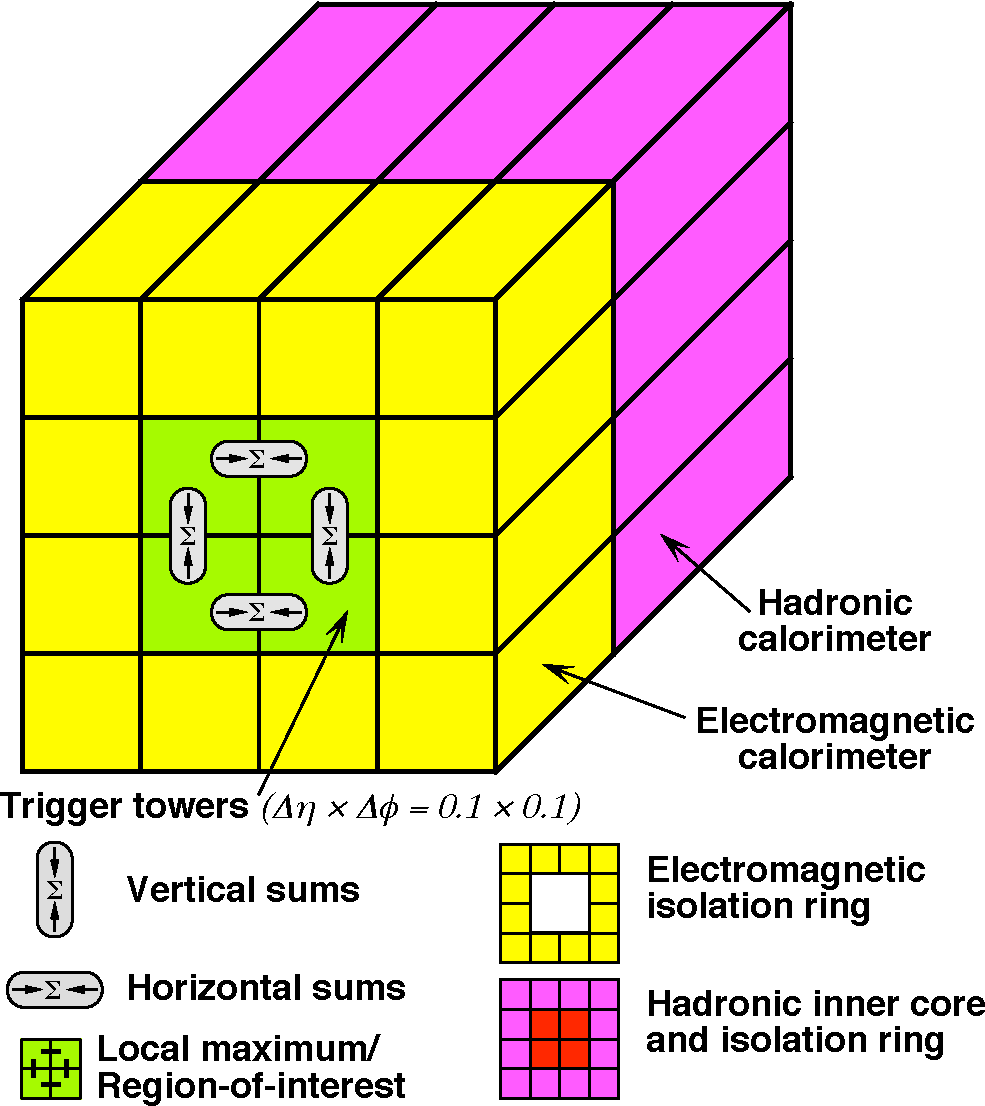
\includegraphics[width=0.4\textwidth]{ATLAS/ATLAS_L1Calo_trigger_tower.pdf}
 \caption[Schematic view of the trigger towers in a region of interest window used as input to the L1Calo trigger algorithms.]{%
  Schematic view of the trigger towers in a RoI window used as input to the L1Calo trigger algorithms~\cite{TRIG-2016-01}.}\label{fig:ATLAS_L1Calo_trigger_tower}
\end{figure}

Simultaneously in L1, the L1Muon trigger uses trigger chambers in the barrel and end-cap regions of the muon spectrometer.
Information from events with large transverse energy are then sent to the L1 topological processor (L1Topo) in the Central Trigger for a trigger decision.
The Central Trigger Processor (CTP) applies a trigger ``menu'' of collections of trigger selections and events that pass these selections are sent to subdetector-specific electronics for processing and data acquisition for possible readout.
Additionally, the L1 trigger defines and sends information on RoIs to the HLT for more detailed decision making.

\subsection{High Level Trigger (HLT)}\label{sec:ATLAS_HLT}

After the L1 trigger acceptance, events sent to the HLT are processed using higher granularity calorimeter information, tracking information from the ID, and precision measurements from the muon spectrometer --- all of which are not available at L1.
The reconstruction and processing in the HLT can utilize both information from the RoIs passed from L1 as well as information received from the full detector subsystems.
Aspects of these processes are elaborated on in \Cref{appendix:bjet_trigger}.


 \chapter{Event Reconstruction}\label{chapter:event_reconstruction}

After physics interactions are detected inside of \gls{ATLAS}, are accepted by the trigger system, and are read out to disk they exist as raw detector level information and need to be reconstructed into detector-based representations of physical particles (physics objects) for analysis.
Low latency versions of reconstruction are done at the trigger level to make acceptance decisions.
However, the full event reconstruction is done ``offline'' later with more current detector models and with computationally expensive algorithms with the luxury of time to trade for great accuracy.
This also allows for reprocessing of data in the future with improved algorithms and models.
This chapter gives a high level overview of the physics objects that ATLAS defines and the methods used to make them.

\section{Tracks}\label{section:tracks}

One of the most common physics objects is charged tracks, as seen in \Cref{fig:track_cartoon}, representing charged particles passing through the subsystems of the \gls{inner detector}, as discussed in \Cref{sec:ATLAS_ID}, and \gls{muon spectrometer}.
These tracks are reconstructed from hits in these subsystems by using the hit coordinates as inputs to fitting algorithms that generally apply $\chi^{2}$ fitting techniques and Kalman filters to find the track that has the highest likelihood for the observed hits~\cite{Fruhwirth:1987fm,Fruhwirth:2003702,Strandlie:1999,Bugge:1981,Salzburger:2008cea}.

\begin{figure}[htbp]
 \centering
 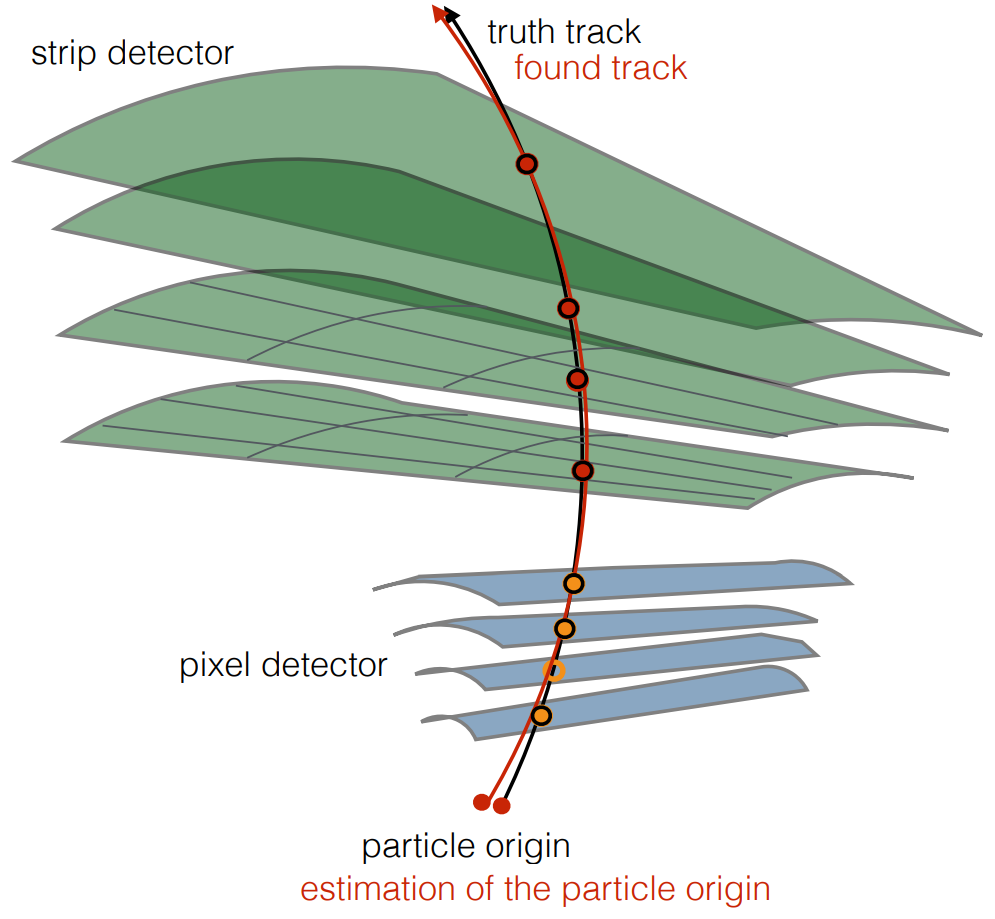
\includegraphics[width=0.8\linewidth]{event_reconstruction/track_cartoon.png}
 \caption[Cartoon of comparison of the ideal charged track to a possible reconstructed charged track.]{%
  Cartoon of comparison of the ideal charged track (\textcolor{black}{black}) in ATLAS from four hits in the pixel layers and four hits in the strip detectors to a possible reconstructed charged track (\textcolor{red}{red}) that accounts for all of the hits except for one hit in the pixel detector~\cite{Salzburger:HammersAndNails}.}
 \label{fig:track_cartoon}
\end{figure}

\section{Electrons and Photons}\label{section:e_gamma}

Reconstruction of electrons begins with the signals arriving from the ECAL cells after they have been reshaped and sampled~\cite{PERF-2013-05}.
These cells are then converted to energy deposit clusters using hardware calibrations, where the ECAL is divided into a grid of towers of size $\Delta \eta \times \Delta \phi = 0.075 \times 0.175$ in the barrel and $\Delta \eta \times \Delta \phi = 0.125 \times 0.125$ in the end-caps to perform sliding-window scans~\cite{Lampl:1099735} to find local maxima to use as seeds for these clusters~\cite{PERF-2013-05}.
Well-reconstructed tracks from the \gls{inner detector} are then matched to the calorimeter clusters.
The matching of tracks is used to infer if the cluster deposits are from prompt%
\footnote{Prompt decays are where a particle originates from the primary interaction.
Prompt decays are distinguished from non-prompt by their decay time.
An example of a prompt electron would be those originating from $Z\to e^{+}e^{-}$, while a non-prompt electron would be an electron that originated from photon conversion from a radiated photon.}
electrons, electrons from photon conversion, or an unconverted photon~\cite{PERF-2013-05,PERF-2016-01}.
If there is no ID track matched to the cluster, the cluster is selected as an unconverted photon.
The fine granularity in $\eta$ of the silicon strip detectors is sufficient to provide event-by-event discrimination between single-photon showers and two overlapping showers originating from the decays of neutral hadrons (mostly $\pi^{0}$ and $\eta$ mesons) in the fiducial region $\abs{\eta} < 1.37$ and $1.52 < \abs{\eta} < 2.37$~\cite{PERF-2017-02}.
If the cluster is matched to a pair of oppositely charged ID tracks that are collinear from the primary vertex and additionally have signatures in the TRT that are consistent with electrons then the clusters are identified as a converted photon.
In all other cases where there are matched ID tracks to calorimeter clusters, the clusters are identified as electrons.

In addition, electrons candidates have additional quality and isolation identification performed.
There are three levels of electron quality ``working points'': \texttt{Loose}, \texttt{Medium}, and \texttt{Tight}.
These working points are effectively minimum values of a multivariate likelihood ratio based discriminate which an analyst can then ``cut'' on to make acceptance decisions.
Isolation criteria are determined using a track-based isolation variable, $p_{T}^{\mathrm{varcone30}}$, and a calorimeter-based isolation variable, $E_{T}^{\mathrm{topcone20}}$.
The isolation criteria compare the scalar sum of the transverse momentum in a cone around the electron candidate track of size $\Delta R < 0.2$ for $E_{T}^{\mathrm{topcone20}}$ and $\Delta R < 0.3$ for $p_{T}^{\mathrm{varcone30}}$ and the transverse momentum of the electron candidate.
This provides an effective discriminant between prompt electron candidates and other electron candidates.

Electrons are also calibrated to data using the well known and characterized resonant decays of $J/\Psi \to e^{+}e^{-}$, $Z \to e^{+}e^{-}$, and $Z \to \ell^{+}\ell^{-}\gamma$.
This calibration is done to derive data-driven \glspl{scale factor} that can be applied to ensure uniformity in the detector response across different subsystems and regions and to establish systematic uncertainties that can cover discrepancies between simulation and data.

\section{Muons}\label{section:muons}

Reconstruction of muons uses tracks from both the \gls{inner detector} and the \gls{muon spectrometer}~\cite{PERF-2015-10}.
The tracks from the ID are reconstructed in the same manner as other charged particles, and the reconstruction algorithms in the MS look for hit patterns in each muon chamber to create unique chamber track segments.
Four muon candidate types are defined based on the combination of subdetectors used in the reconstruction.
Combined (CB) muons are constructed from combined, global refits of the ID and MS tracks by adding or removing tracks from the MS to improve the quality of the fit.
Segment-tagged (ST) muons are constructed by identifying tracks in the ID as muon tracks if there is an associated track to it in the \gls{MDT} or \gls{CSC}.
ST muon candidates are primarily low $p_{T}$ muons that do not traverse the entire MS.
Calorimeter-tagged (CT) muons are constructed from ID tracks and an ECAL deposit consistent with a minimum ionizing particle.
Extrapolated (ME) muons are constructed from MS tracks in at least two layers that point back to the primary vertex.
ME muon candidates are used to extend the acceptance of muon reconstruction outside the ID in the region of $2.5 < \abs{\eta} < 2.7$ where there is no ID coverage.
With regards to priority when there is overlap of muons of various categories, more information is preferred and so the (decreasing) priority ordering is CB, ST, CT.
If there is overlap with ME muons additional track quality information is required to resolve priority.

Like electrons, muon quality working points are established, and four are used in ATLAS.
For the \texttt{loose} working point all muon types are used.
This is useful for analyses where it is beneficial to maximize reconstruction efficiency above other concerns, such as $H \to 4\ell$.
The \texttt{medium} working point CB and ME tracks are used where there are at least three CB track hits and three ME layers.
The \texttt{tight} working point is designed to maximize muon purity and only used CB muons which have hits in at least two layers of the MS and also satisfy the \texttt{medium} working point requirements.
Finally, the high-$p_{T}$ working point requires CB muons passing the \texttt{medium} selection with at least three hits in the MS.
This working point is designed to maximize the momentum resolution for muon tracks with $p_{T} > 100~\GeV$.
Additionally, there are muon isolation requirements.
These isolation requirements use the track-based isolation variable, $p_{T}^{\mathrm{varcone30}}$, and a calorimeter-based isolation variable, $E_{T}^{\mathrm{topcone20}}$, described in \Cref{section:e_gamma}.
Muons are also further calibrated to data using $J/\Psi \to \mu^{+}\mu^{-}$ to cover the low $p_{T}$ spectrum and $Z \to \mu^{+}\mu^{-}$ for the high $p_{T}$ spectrum, as shown in \Cref{fig:dimuon_efficiency_scale_factor_uncert}.

\begin{figure}[htbp]
 \centering
 \includegraphics[width=0.8\linewidth]{event_reconstruction/dimuon_efficiency_scale_factor_uncert.eps}
 \caption[Total uncertainty in the efficiency scale factor for Medium muons as a function of $p_{T}$ as obtained from $Z\to\mu\mu$ and $J/\Psi \to \mu\mu$ decays.]{%
  Total uncertainty in the efficiency scale factor for Medium muons as a function of $p_{T}$ as obtained from $Z\to\mu\mu$ (solid lines) and $J/\Psi \to \mu\mu$ (dashed lines) decays.
  The combined uncertainty is the sum in quadrature of the individual contributions~\cite{PERF-2015-10}.}
 \label{fig:dimuon_efficiency_scale_factor_uncert}
\end{figure}

\section{Jets}\label{section:jets}

As particles that carry \gls{QCD} color charge do not exist by themselves in isolation, but combine with other colored particles to form colorless composite particles known as ``hadrons,'' it is not possible to directly observe quarks or gluons in ATLAS.
Instead, this process of hadronization, and subsequent decays and rehadronization, creates a shower of both charged and neutral particles that hit the detector, creating charged tracks and energy deposits.
These hadronic showers are stochastic, and there is no way to give a full descriptive definition of them, though there is very impressive recent work on operational definitions~\cite{Metodiev:2018ftz,Komiske:2018vkc,Larkoski:2019nwj}.
Instead, clustering algorithms are used to create collections of tracks and energy deposits, known as ``jets'', based off of the criteria of interest in the algorithm.
In a similar manner to how QCD's depth and richness as a theory requires proper treatment outside the scope of this thesis, jet physics is complex and deep enough to rightly be its own intense physics program at the LHC.
This section will only attempt to give an executive summary of the jet physics and techniques that is pertinent to my thesis analysis --- however for an exceedingly thorough overview see~\cite{Nachman:2016qyc}.

Of the jet clustering algorithms that are common in high energy physics~\cite{Salam:2009jx,Salam:2007xv} the most widely used are the $k_{t}$, Cambridge/Aachen, and anti-$k_{t}$ algorithms~\cite{Cacciari:2008gp,Soyez:2008pq}.
These algorithms are all similar in their approaches with variations on the features they emphasize.
The approach is to iteratively apply the following for all objects in the considered RoI:
\begin{enumerate}
 \item Compute the pairwise distance $d_{ij}$ between objects $i$ and $j$ where
       \[
        d_{ij} = \textrm{min}\left(k_{ti}^{2p}, k_{tj}^{2p}\right) \frac{\Delta_{ij}^{2}}{R^{2}}
       \]
       and $\Delta_{ij}^{2} = \left(y_{i} - y_{j}\right)^{2} + \left(\phi_{i} - \phi_{j}\right)^{2}$ for transverse momentum $k_{t}$, rapidity $y$, and azimuthal angle $\phi$, and parameters of choice $R$, which governs the size of the jet (though it is not a hard cutoff limit), and $p$, which governs the relative power of the energy versus geometrical $\left(\Delta_{ij}\right)$ scales~\cite{Cacciari:2008gp}.
 \item Compute the distance $d_{iB}$ between the object $i$ and the beamline $B$ where $d_{iB} = k_{ti}^{2p}$.
 \item Determine the smallest distance out of the set of distances $d_{ij}$ and $d_{iB}$, $d_{\mathrm{min}} \in \left\{\left\{d_{ij}\right\},\left\{d_{iB}\right\}\right\}$.
 \item If the minimum distance is between the object $i$ and the beamline, $d_{\mathrm{min}} \in \left\{d_{iB}\right\}$, label this object a jet and remove it.
 \item If the minimum distance is between object $i$ and $j$, $d_{\mathrm{min}} \in \left\{d_{ij}\right\}$, group these two objects into a new object $k$ which is added to the object collection, and remove objects $i$ and $j$.
\end{enumerate}
The above is repeated until there are no more remaining objects, at which point all objects have been assigned to a jet.
It is seen that the choice of free parameter $p$ then defines which algorithm is used, and what information the jet clustering algorithm prioritizes.
The choice of $p=1$ corresponds to the $k_{t}$ algorithm~\cite{Catani:1993hr}, which is seen to cluster softer --- less energetic --- objects together into progressively harder --- more energetic --- objects, as seen in \Cref{fig:jet_algorithms_kt}.
Working under the assumption that generally the hardest objects will be towards the center of the shower of particles, this can be seen as an ``outside-in'' clustering which will result in irregularly shaped (probably not very cone-like) jets.
Choosing $p=0$ corresponds to the Cambridge/Aachen jet algorithm~\cite{Dokshitzer:1997in}, which reduces the distance $d_{ij}$ to only include the angular information, $\Delta_{ij}$.
This means that softer splittings of the shower will be clustered into harder branches, which will again produce irregular shaped jets, as seen in \Cref{fig:jet_algorithms_Cambridge_Aachen}.
Choosing $p=-1$ corresponds to the anti-$k_{t}$ algorithm~\cite{Cacciari:2008gp}, where the hardest objects are clustered together first and then subsequently softer objects are added.
The anti-$k_{t}$ algorithm produces relatively regular cone shaped jets that are focused around a hard core, as seen in \Cref{fig:jet_algorithms_anti_kt}.
A typical choice of jet algorithm in ATLAS is the anti-$k_{t}$ algorithm with size parameter of $R=0.4$.

\begin{figure}[htbp]
 \centering
 \begin{subfigure}[t]{0.315\textwidth}
  \centering
  \includegraphics[width=\textwidth]{event_reconstruction/kt.eps}
  \caption[The sample parton-level event clustered with the $k_{t}$ jet algorithm.]{%
   The sample parton-level event clustered with the $k_{t}$ jet algorithm.}
  \label{fig:jet_algorithms_kt}
 \end{subfigure}%
 \quad
 \begin{subfigure}[t]{0.315\textwidth}
  \centering
  \includegraphics[width=\textwidth]{event_reconstruction/Cambridge_Aachen.eps}
  \caption[The sample parton-level event clustered with the Cambridge/Aachen jet algorithm.]{%
   The sample parton-level event clustered with the Cambridge/Aachen jet algorithm.}
  \label{fig:jet_algorithms_Cambridge_Aachen}
 \end{subfigure}%
 \quad
 \begin{subfigure}[t]{0.315\textwidth}
  \centering
  \includegraphics[width=\textwidth]{event_reconstruction/anti_kt.eps}
  \caption[The sample parton-level event clustered with the anti-$k_{t}$ jet algorithm.]{%
   The sample parton-level event clustered with the anti-$k_{t}$ jet algorithm.}
  \label{fig:jet_algorithms_anti_kt}
 \end{subfigure}%
 \caption[A sample parton-level event, together with many random soft ``ghosts'', clustered with three different jet algorithms, illustrating the ``active'' catchment areas of the resulting hard jets.]{%
  A sample parton-level event (generated with Herwig), together with many random soft ``ghosts'', clustered with the $k_{t}$, Cambridge/Aachen, and anti-$k_{t}$ jet algorithms, illustrating the ``active'' catchment areas of the resulting hard jets.
  For $k_{t}$ and Cambridge/Aachen the detailed shapes are in part determined by the specific set of ghosts used, and change when the ghosts are modified~\cite{Cacciari:2008gp}.}
 \label{fig:jet_algorithms}
\end{figure}


\subsection{Large Radius Jets}\label{subsection:largeR_jets}

For analyses that are dealing with very high momentum resonances, the resulting decay products can become highly collimated and be reconstructed as a single jet with a large radius parameter, $R$, (a ``\largeR{}'' jet) typically set to $R=1.0$~\cite{JETM-2018-02,SUSY-2016-13}.
For my thesis analysis \largeR{} jets were used, where the \largeR{} jets were reconstructed from topological clusters in the calorimeters using the anti-$k_{t}$ algorithm with radius parameter of $R=1.0$ and were trimmed~\cite{Krohn:2009th} to improve mass resolution and reduce dependence on pile-up.
The trimming is done by reclustering the \largeR{} jet constituents using the $k_{t}$ algorithm with a radius parameter of $R=0.2$ into subjets, and then removing any subjet that has $p_{T}$ less than $5\%$ of the \largeR{} parent jet's energy.

\subsection{Variable Radius Track Jets}\label{subsection:VR_jets}

In recent years there have been dedicated efforts to improve jet algorithm techniques, especially in the high momentum regime.
As part of these efforts, variable radius (VR) jets~\cite{Krohn:2009zg,ATL-PHYS-PUB-2017-010} were introduced where the radius parameter, $R$, decreases as a function of the jet $p_{T}$,
\[
 R_{\mathrm{eff}} \left(p_{T}\right)= \frac{\rho}{p_{T}},
\]
where the dimensionful constant $\rho$ determines how fast the effective jet size decreases with the transverse momentum of the jet.
The choice of $\rho$ should be proportional to the mass of the resonance, and so should correctly reproduce the size of jets as long as $\rho \lesssim 2 p_{T}$.
Additional parameters $R_{\mathrm{min}}$ and $R_{\mathrm{max}}$ are used to to impose
lower and upper cut-offs on the jet size,
\[
 R_{\mathrm{eff}} \left(p_{T}\right)= \mathrm{max}\left[\mathrm{min}\left(\frac{\rho}{p_{T}},R_{\mathrm{max}}\right),R_{\mathrm{min}}\right]\,.
\]
For my thesis analysis variable radius track jets~\cite{Zenz:2010hfa} were used with $\rho=30~\GeV$, $R_{\mathrm{min}}=0.02$, and $R_{\mathrm{max}}=0.4$, which in simulation gives the highest truth subjet double $b$-labelling efficiency for high $p_{T}$ Higgs bosons~\cite{ATL-PHYS-PUB-2017-010}, as seen in \Cref{fig:VR_jets_parameters}.
It is seen from \Cref{fig:VR_jets_lead_subjet}, \Cref{fig:VR_jets_sublead_subjet}, and \Cref{fig:Higgs_VR_DeltaR} that VR track jets are able to describe the topology of $\Hbb$ events across high $p_{T}$ spectrum much more accurately than fixed radius $R=0.2$ track jets, making their use an excellent choice for the analysis.

\begin{figure}[htbp]
 \centering
 \begin{subfigure}[t]{0.48\textwidth}
  \centering
  \includegraphics[width=\textwidth]{event_reconstruction/VR_jets_rho_values.eps}
  \caption[The efficiency for VR track jets with ${R_{\mathrm{min}}=0.02}$ and ${R_{\mathrm{max}} = 0.4}$ for several $\rho$ values.]{%
   The efficiency for VR track jets with ${R_{\mathrm{min}}=0.02}$ and ${R_{\mathrm{max}} = 0.4}$ for several $\rho$ values.}
  \label{fig:VR_jets_rho_values}
 \end{subfigure}%
 \quad
 \begin{subfigure}[t]{0.48\textwidth}
  \centering
  \includegraphics[width=\textwidth]{event_reconstruction/VR_jets_Rmin.eps}
  \caption[The efficiency for VR track jets with ${\rho=30~\GeV}$ and ${R_{\mathrm{max}} = 0.4}$ for different values of $R_{\mathrm{min}}$.]{%
   The efficiency for VR track jets with ${\rho=30~\GeV}$ and ${R_{\mathrm{max}} = 0.4}$ for different values of $R_{\mathrm{min}}$.}
  \label{fig:VR_jets_Rmin}
 \end{subfigure}%

 \begin{subfigure}[t]{0.48\textwidth}
  \centering
  \includegraphics[width=\textwidth]{event_reconstruction/VR_jets_Rmax.eps}
  \caption[The efficiency for VR track jets with ${\rho=30~\GeV}$ and ${R_{\mathrm{min}} = 0.02}$ for varying values of $R_{\mathrm{max}}$.]{%
   The efficiency for VR track jets with ${\rho=30~\GeV}$ and ${R_{\mathrm{min}} = 0.02}$ for varying values of $R_{\mathrm{max}}$.}
  \label{fig:VR_jets_Rmax}
 \end{subfigure}%
 \caption[Efficiency of subjet double $b$-labelling at the truth level of a Higgs jet as a function of the Higgs jet $p_{T}$.]{%
  Efficiency of subjet double $b$-labelling at the truth level of a Higgs jet as a function of the Higgs jet $p_{T}$.
  The efficiency for $R=0.2$ track jets is also included in all of the plots.
  The uncertainty bars include statistical uncertainties only~\cite{ATL-PHYS-PUB-2017-010}.}
 \label{fig:VR_jets_parameters}
\end{figure}

\begin{figure}[htbp]
 \centering
 \begin{subfigure}[t]{0.48\textwidth}
  \centering
  \includegraphics[width=\textwidth]{event_reconstruction/VR_jets_lead_subjet_low.eps}
  \caption[Distributions of the $\Delta R$ between leading subjets and matched truth $b$-hadrons for Higgs with low jet $p_{T}$ of ${250~\GeV < p_{T} < 400~\GeV}$.]{%
   Distributions of the $\Delta R$ between leading subjets and matched truth $b$-hadrons for Higgs with low jet $p_{T}$ of ${250~\GeV < p_{T} < 400~\GeV}$.}
  \label{fig:VR_jets_lead_subjet_low}
 \end{subfigure}%
 \quad
 \begin{subfigure}[t]{0.48\textwidth}
  \centering
  \includegraphics[width=\textwidth]{event_reconstruction/VR_jets_lead_subjet_high.eps}
  \caption[Distributions of the $\Delta R$ between leading subjets and matched truth $b$-hadrons for Higgs with high jet $p_{T}$ of ${800~\GeV < p_{T} < 1000~\GeV}$.]{%
   Distributions of the $\Delta R$ between leading subjets and matched truth $b$-hadrons for Higgs with high jet $p_{T}$ of ${800~\GeV < p_{T} < 1000~\GeV}$.}
  \label{fig:VR_jets_lead_subjet_high}
 \end{subfigure}%
 \caption[Distributions of the $\Delta R$ between leading subjets and matched truth $b$-hadrons for two different Higgs jet $p_{T}$ bins.]{%
  Distributions of the $\Delta R$ between leading subjets and matched truth $b$-hadrons for low Higgs jet $p_{T}$ of ${250~\GeV < p_{T} < 400~\GeV}$ and high Higgs jet $p_{T}$ of ${800~\GeV < p_{T} < 1000~\GeV}$.
  The uncertainty bars include statistical uncertainties only.
  All algorithms have been normalized to an area corresponding to the fraction of signal jets which contain a leading subjet~\cite{ATL-PHYS-PUB-2017-010}.}
 \label{fig:VR_jets_lead_subjet}
\end{figure}

\begin{figure}[htbp]
 \centering
 \begin{subfigure}[t]{0.48\textwidth}
  \centering
  \includegraphics[width=\textwidth]{event_reconstruction/VR_jets_sublead_subjet_low.eps}
  \caption[Distributions of the $\Delta R$ between subleading subjets and matched truth $b$-hadrons for Higgs with low jet $p_{T}$ of ${250~\GeV < p_{T} < 400~\GeV}$.]{%
   Distributions of the $\Delta R$ between subleading subjets and matched truth $b$-hadrons for Higgs with low jet $p_{T}$ of ${250~\GeV < p_{T} < 400~\GeV}$.}
  \label{fig:VR_jets_sublead_subjet_low}
 \end{subfigure}%
 \quad
 \begin{subfigure}[t]{0.48\textwidth}
  \centering
  \includegraphics[width=\textwidth]{event_reconstruction/VR_jets_sublead_subjet_high.eps}
  \caption[Distributions of the $\Delta R$ between subleading subjets and matched truth $b$-hadrons for Higgs with high jet $p_{T}$ of ${800~\GeV < p_{T} < 1000~\GeV}$.]{%
   Distributions of the $\Delta R$ between subleading subjets and matched truth $b$-hadrons for Higgs with high jet $p_{T}$ of ${800~\GeV < p_{T} < 1000~\GeV}$.}
  \label{fig:VR_jets_sublead_subjet_high}
 \end{subfigure}%
 \caption[Distributions of the $\Delta R$ between subleading subjets and matched truth $b$-hadrons for two different Higgs jet $p_{T}$ bins.]{%
  Distributions of the $\Delta R$ between subleading subjets and matched truth $b$-hadrons for low Higgs jet $p_{T}$ of ${250~\GeV < p_{T} < 400~\GeV}$ and high Higgs jet $p_{T}$ of ${800~\GeV < p_{T} < 1000~\GeV}$.
  The uncertainty bars include statistical uncertainties only.
  All algorithms have been normalized to an area corresponding to the fraction of signal jets which contain a leading subjet~\cite{ATL-PHYS-PUB-2017-010}.}
 \label{fig:VR_jets_sublead_subjet}
\end{figure}

\begin{figure}[htbp]
 \centering
 \includegraphics[width=0.8\linewidth]{event_reconstruction/Higgs_VR_DeltaR.eps}
 \caption[The $\Delta R$ between the two leading truth $b$-hadrons or subjets associated to Higgs jets as a function of Higgs jet $p_{T}$.]{%
  The $\Delta R$ between the two leading truth $b$-hadrons or subjets associated to Higgs jets as a function of Higgs jet $p_{T}$~\cite{Salzburger:HammersAndNails}.}
 \label{fig:Higgs_VR_DeltaR}
\end{figure}

\section{Flavor Tagging}\label{section:flavor_tagging}

Flavor tagging of jets is the process of determining a ``flavor'' label --- light, charm $(c)$, or bottom $(b)$ --- to characterize the type of hadrons in the hadronic shower that resulted in the jet.
Flavor tagging is vital in precision measurements in the top quark sector%
\footnote{Noting that the top quark has a branching fraction of $\mathcal{B}\left(t \to W b\right) = 0.96_{-0.066}^{+0.068}\left(\mathrm{stat.}\right)_{-0.052}^{+0.064}\left(\mathrm{syst.}\right)$~\cite{Abazov:2010tm,PhysRevD.98.030001}.}%
, in the search for the Higgs boson as well as new phenomena decaying to $b\bar{b}$ states, and, in particular importance to this thesis analysis, the suppression of background processes that contain predominantly light-flavor jets~\cite{PERF-2012-04}.
Of particular great interest in flavor tagging is $b$-tagging (labeling of jets containing $b$-hadrons --- $b$-jets), as $b$-hadrons are often produced in decays of heavy resonances that could be indicative of interesting new physics.
$b$-hadrons have a number of unique properties that distinguish them, as seen in \Cref{fig:b_jet}.
Notable among them is their long lifetime, discussed in \Cref{appendix:B_hadron_lifetimes}, of approximately $1.5~\mathrm{ps}$ which gives a characteristic length scale of $c\tau \sim 0.45~\mathrm{mm}$.
This is a significant enough flight distance of the $B$ meson before it decays, that this subsequent hadron shower and jet is viewed as having a secondary vertex (SV) displaced from the original jet vertex.
This secondary vertex is detectable as the vertex resolution in ATLAS for $50$ associated tracks is approximately $20~\mu\mathrm{m}$ in $r$-$\phi$ by $30~\mu\mathrm{m}$ in $z$~\cite{Choi:2271033,ATL-PHYS-PUB-2015-026}.
$B$ mesons also have a mass of approximately $5~\GeV$.
Collectively, these properties can be exploited by $b$-tagging algorithms to discriminate $b$-jets from light or charm jets~\cite{ATL-PHYS-PUB-2015-022,ATL-PHYS-PUB-2016-012,ATL-PHYS-PUB-2017-013,PERF-2016-05}.

\begin{figure}[htbp]
 \centering
 \centering
 \includegraphics[width=0.6\textwidth]{event_reconstruction/b_jet.pdf}
 \caption[Cartoon of a typical $b$-jet.]{%
  Cartoon of a typical $b$-jet containing a $b$-hadron decay vertex (\textcolor{track_blue}{blue}~\tikzdot{track_blue}) displaced from the primary $pp$ vertex (\textcolor{red}{red}~\tikzdot{red}), and a $c$-hadron decay vertex (\textcolor{orange}{orange}~\tikzdot{orange}) further displaced and often close to the $b$-hadron flight axis.
  Tracks from secondary (\textcolor{track_blue}{blue}) and tertiary (\textcolor{orange}{orange}) vertices have large impact parameters (\textcolor{IPgreen}{green}) with respect to the primary $pp$ vertex~\cite{Chisholm:bjet}.}
 \label{fig:b_jet}
\end{figure}

It is seen from \Cref{fig:signed_impact_parameters} that the transverse and longitudinal impact parameters --- respectively, $d_{0}$ and $z_{0}$ --- of $b$-jets tend to be positive, while $c$-jets and light-jets tend to have more impact parameters distributed more symmetrically around $0$.
As a result, these impact parameters can be used as inputs to discriminating algorithms.
For the data taking periods of my thesis analysis the main $b$-tagging algorithm used in ATLAS was the \texttt{MV2c10} \gls{BDT} based algorithm.%
\footnote{\texttt{MV2c10} is named to reflect that it is a multivariate algorithm with the fraction of $c$-jets in the training sample at roughly $10\%$.
 In reality the $c$-jet fraction is $7\%$ and the light-jet fraction is $93\%$ to give a good balance between light-jet and $c$-jet rejection.}
In addition to the quantities of the jet itself, \texttt{MV2c10} uses the output of other lower level $b$-tagging algorithms as inputs, as seen in \Cref{fig:MV2_inputs}.
These include the likelihood ratio based two-dimensional and three-dimensional impact parameter algorithms, IP2D and IP3D.
The IP2D and IP3D algorithms assume that the track IPs are uncorrelated.
The output of IP3D is shown in \Cref{fig:IP3D_LLR} for the 2017 and 2018 data taking optimization of using a training sample of $50\%$ $t\bar{t}$ and $50\%$ $\Zprime \to q\bar{q}$ for $q\in\left\{\mathrm{light}, c, b\right\}$ to cover a large $p_{T}$ range of jets.
The 2016 optimization used a training sample of $50\%$ $t\bar{t}$ and $50\%$ $\Zprime \to t\bar{t}$.
In the 2017 data taking a Recurrent Neural Network (RNN) impact parameter tagger (RNNIP)~\cite{ATL-PHYS-PUB-2017-003} was added as well, that exploits the correlations between the impact parameters between the tracks, as $b$-jets tend to have multiple highly significant IP tracks, while this is not the case for light flavor jets, as seen in \Cref{fig:RNNIP_track_significance}.
There are additional displaced secondary vertex finding algorithms (SV1), and Kalman filter algorithms (JetFitter) that exploit that roughly $90\%$ of $b$-jets contain a $c$-jet and so follow this decay chain.
Additionally a Soft Muon Tagger is also added which in the 2017 data taking based on
the reconstruction of muons from the semileptonic decay of $b$-hadrons and $c$-hadrons.
The \texttt{MV2c10} BDT combines all these inputs and then gives a discriminant score indicative of how $b$-jet-like or how un-$b$-jet-like the inputs are given its training, as seen in \Cref{fig:MV2c10_BDT}.
The \texttt{MV2c10} BDT is trained using $t\bar{t}$ for the 2016 optimization, and a hybrid sample of $t\bar{t}$ and $\Zprime$ to cover a wide $p_{T}$ spectrum for the 2017 optimization.
The performance of the BDT is calibrated in data using jets that contain a muon, indicative of the semileptonic decay of a $b$-hadron, and a correction scale factor is derived.

\begin{figure}[htbp]
 \centering
 \centering
 \includegraphics[width=\textwidth]{event_reconstruction/MV2_inputs.pdf}
 \caption[Inputs to the high level $b$-tagging algorithm \texttt{MV2c10} for data taking in 2017 and 2018.]{%
  Inputs to the high level $b$-tagging algorithm \texttt{MV2c10} for data taking in 2017 and 2018~\cite{Feickert:ML4Jets2018}.
  The RNNIP was added in 2017 and so for the 2015 and 2016 data taking JetFitter was used instead.}
 \label{fig:MV2_inputs}
\end{figure}

\begin{figure}[htbp]
 \centering
 \begin{subfigure}[t]{0.48\textwidth}
  \centering
  \includegraphics[width=\textwidth]{event_reconstruction/IP3D_d0_2016.eps}
  \caption[Transverse impact parameter significance values for the 2016 configuration of the IP3D algorithm.]{%
   Data-MC comparisons of the transverse impact parameter significance values for the 2016 configuration of the IP3D algorithm.}
  \label{fig:IP3D_d0_2016}
 \end{subfigure}%
 \quad
 \begin{subfigure}[t]{0.48\textwidth}
  \centering
  \includegraphics[width=\textwidth]{event_reconstruction/IP3D_d0_2017.eps}
  \caption[Transverse impact parameter significance values for the 2017 configuration of the IP3D algorithm.]{%
   Data-MC comparisons of the transverse impact parameter significance values for the 2017 configuration of the IP3D algorithm.}
  \label{fig:IP3D_d0_2017}
 \end{subfigure}%

 \begin{subfigure}[t]{0.48\textwidth}
  \centering
  \includegraphics[width=\textwidth]{event_reconstruction/IP3D_z0_2016.eps}
  \caption[Longitudinal impact parameter significance values for the 2016 configuration of the IP3D algorithm.]{%
   Data-MC comparisons of the longitudinal impact parameter significance values for the 2016 configuration of the IP3D algorithm.}
  \label{fig:IP3D_z0_2016}
 \end{subfigure}%
 \quad
 \begin{subfigure}[t]{0.48\textwidth}
  \centering
  \includegraphics[width=\textwidth]{event_reconstruction/IP3D_z0_2017.eps}
  \caption[Longitudinal impact parameter significance values for the 2017 configuration of the IP3D algorithm.]{%
   Data-MC comparisons of the longitudinal impact parameter significance values for the 2017 configuration of the IP3D algorithm.}
  \label{fig:IP3D_z0_2017}
 \end{subfigure}%
 \caption[Data-Monte Carlo comparisons of the transverse and longitudinal impact parameter significance values for IP3D selected tracks in the leading jet of the $Z\to\mu\mu + \textrm{jets}$ dominated sample.]{%
  Data-Monte Carlo comparisons of the transverse and longitudinal impact parameter significance values for IP3D selected tracks in the leading jet of a $Z\to\mu\mu + \textrm{jets}$ dominated sample~\cite{ATL-PHYS-PUB-2017-013}.}
 \label{fig:signed_impact_parameters}
\end{figure}

\begin{figure}[htbp]
 \centering
 \begin{subfigure}[t]{0.48\textwidth}
  \centering
  \includegraphics[width=\textwidth]{event_reconstruction/IP3D_LLR_ttbar.eps}
  \caption[Data-Monte Carlo comparison of the IP3D log-likelihood ratio using a $t\bar{t}$-dominated $e\mu$ sample.]{%
   Data-Monte Carlo comparison of the IP3D log-likelihood ratio using a $t\bar{t}$-dominated $e\mu$-dominated sample.}
  \label{fig:IP3D_LLR_ttbar}
 \end{subfigure}%
 \quad
 \begin{subfigure}[t]{0.48\textwidth}
  \centering
  \includegraphics[width=\textwidth]{event_reconstruction/IP3D_LLR_Zjets.eps}
  \caption[Data-Monte Carlo comparison of the IP3D log-likelihood ratio using a $Z\to \mu^{+}\mu^{-}+\textrm{jets}$-dominated sample.]{%
   Data-Monte Carlo comparison of the IP3D log-likelihood ratio using a $Z\to \mu^{+}\mu^{-}+\textrm{jets}$-dominated sample.}
  \label{fig:IP3D_LLR_Zjets}
 \end{subfigure}%
 \caption[Data-Monte Carlo comparison of the log-likelihood ratio used to discriminate the $b$-jet from the light-flavour jet hypotheses in the IP3D $b$-tagging algorithm using different samples.]{%
  Data-Monte Carlo comparison of the log-likelihood ratio used to discriminate the $b$-jet from the light-flavour jet hypotheses in the IP3D $b$-tagging algorithm using a $t\bar{t}$-dominated $e\mu$ sample and a ${Z\to \mu^{+}\mu^{-}+\textrm{jets}}$-dominated sample~\cite{ATL-PHYS-PUB-2017-013}.}
 \label{fig:IP3D_LLR}
\end{figure}

\begin{figure}[htbp]
 \centering
 \begin{subfigure}[t]{0.48\textwidth}
  \centering
  \includegraphics[width=\textwidth]{event_reconstruction/d0_sig_correlations_bjet.pdf}
  \caption[The distribution of the $d_{0}$ significance for the leading $d_{0}$ significance track and subleading $d_{0}$ significance track in $b$-jets jets.]{%
   The distribution of the $d_{0}$ significance for the leading $d_{0}$ significance track and subleading $d_{0}$ significance track in $b$-jets jets.}
  \label{fig:d0_sig_correlations_bjet}
 \end{subfigure}%
 \quad
 \begin{subfigure}[t]{0.48\textwidth}
  \centering
  \includegraphics[width=\textwidth]{event_reconstruction/d0_sig_correlations_lightjet.pdf}
  \caption[The distribution of the $d_{0}$ significance for the leading $d_{0}$ significance track and subleading $d_{0}$ significance track in light jets.]{%
   The distribution of the $d_{0}$ significance for the leading $d_{0}$ significance track and subleading $d_{0}$ significance track in light jets.}
  \label{fig:d0_sig_correlations_lightjet}
 \end{subfigure}%
 \caption[The distribution of the $d_{0}$ significance for the leading $d_{0}$ significance track and subleading $d_{0}$ significance track in $b$-jets and light jets.]{%
  The distribution of the $d_{0}$ significance for the leading $d_{0}$ significance track and subleading $d_{0}$ significance track in $b$-jets and light jets.
  The distributions were produced with 700 thousand $b$-jets and 1 million light jets, and each distribution is normalized to unity~\cite{ATL-PHYS-PUB-2017-003}.}
 \label{fig:RNNIP_track_significance}
\end{figure}

\begin{figure}[htbp]
 \centering
 \begin{subfigure}[t]{0.48\textwidth}
  \centering
  \includegraphics[width=\textwidth]{event_reconstruction/MV2c10_BDT_output.eps}
  \caption[The \texttt{MV2c10} output for $b$-jets, $c$-jets, and light-flavor jets in simulated $t\bar{t}$ events.]{%
   The \texttt{MV2c10} output for $b$-jets (solid line), $c$-jets (dashed line), and light-flavor jets (dotted line) in simulated $t\bar{t}$ events.}
  \label{fig:MV2c10_BDT_output}
 \end{subfigure}%
 \quad
 \begin{subfigure}[t]{0.48\textwidth}
  \centering
  \includegraphics[width=\textwidth]{event_reconstruction/MV2c10_background_rejection.eps}
  \caption[The light-flavor jet and $c$-jet rejection factors as a function of the $b$-jet tagging efficiency of the \texttt{MV2c10} $b$-tagging algorithm.]{%
   The light-flavor jet (dashed line) and $c$-jet rejection factors (solid line) as a function of the $b$-jet tagging efficiency of the \texttt{MV2c10} $b$-tagging algorithm.}
  \label{fig:MV2c10_background_rejection}
 \end{subfigure}%
 \caption[The performance of the \texttt{MV2c10} BDT $b$-tagging algorithm in simulated $t\bar{t}$ events.]{%
  The performance of the \texttt{MV2c10} BDT $b$-tagging algorithm in simulated $t\bar{t}$ events.
  The performance was evaluated on $t\bar{t}$ events simulated using \textsc{Powheg} interfaced to \textsc{Pythia6}~\cite{PERF-2016-05}.}
 \label{fig:MV2c10_BDT}
\end{figure}

\clearpage
\section{Taus}\label{section:taus}

Tau leptons also produced in collisions in ATLAS, however, given their short lifetime they will decay into other SM particles before entering the detector subsystems and are reconstructed as other physics objects.
When taus decay they decay to hadrons approximately $64\%$ of the time~\cite{Gallinaro:2014eha}, and to other leptons $36\%$ of the time.
The leptonic decays are reconstructed as muons or electrons, and the hadronic decay modes, usually to pions, they are reconstructed as multi-pronged jets matched with tracks in the ID.
As hadronic decays of the tau also have a displaced secondary vertex they can be a source of fakes for $b$-jets.

\section{Missing Transverse Momentum}\label{section:MET}

Missing transverse momentum, $\MET$ --- or ``MET'' --- is the imbalance of momentum in the transverse plane of the event.
Any event that has neutrinos produced in it, such as events with $W \to \ell \nu_{\ell}$ processes, will have $\MET$ as neutrinos pass through ATLAS without interaction, escaping detection.
However, in events without neutrinos if other physics objects are not properly reconstructed there will still be some $\MET$ in the event due to acceptance and efficiency effects.

In closing, given the fully hadronic signature of the analysis signature in the high momentum regime, that will be described in \Cref{chapter:analysis}, and the use of $b$-tagging it is seen that the proper reconstruction of \largeR{} jets with $b$-tagged VR subjets is going to be of great importance.
Additionally, well reconstructed muons will play an important role in the establishment of a $t\bar{t}$ control region.


 \chapter{Search for boosted low mass resonances in the $b\bar{b}$ final state}\label{chapter:analysis}

This chapter describes the analysis that was performed for a search for high momentum (``boosted'') low mass resonances, $X$, decaying to $b\bar{b}$ with an additional jet using $80.5~\ifb$ of $\sqrt{s} = 13~\TeV$ data from the ATLAS detector.
In addition to the overview and description of the analysis the chapter will also focus on my contributions to modeling the irreducible multijet continuum background --- the dominant background of the analysis.

Extensive analyses searching for dijet resonances have been performed by ATLAS and CMS in Run 2 of the LHC~\cite{EXOT-2016-21,CMS-EXO-16-032,CMS-EXO-16-046}, though the focus of these analyses were high mass resonances above $1~\TeV$, where the search sensitivity and range is largely dictated by the LHC center-of-mass energy.
This leaves the sub-$\mathrm{TeV}$ mass range as a possible landscape for new resonances with small couplings to SM particles, such as $\Zprime$ bosons as seen in \Cref{fig:darkmatter_coupling_summary} and \Cref{fig:CMS_dijet_summary}.
Probing low mass regions imposes its own set of challenges, as low mass resonances can produce lower energy final states, which in the high event rate environment of the LHC can be difficult to distinguish and trigger on as most proton-proton collisions at the LHC are soft interactions that result in many low momentum jets.\footnote{%
 This is reflected in the large cross section for jets and di-jet events shown in \Cref{fig:cross_section_experiment_theory}.}
In particular for dijet analyses, this introduces an enormous multijet background produced by QCD interactions, as seen in \Cref{fig:SM_fiducial_cross_section_summary}.
Requiring that the transverse momentum of these resonances is very large (highly boosted) offers a path forward to both triggering on the interesting signal events and also reducing the multijet background which exponentially falls off with increasing momentum.
To achieve this highly boosted state, the resonance can recoil off a high energy jet or photon~\cite{EXOT-2017-01} that is produced through initial state radiation (ISR) or another similar process, as shown at the leading order in Feynman diagrams in \Cref{fig:signal_LO_diagrams} for signal models of a leptophobic $\Zprime$ and the Higgs boson at the LHC.
For this thesis analysis only the jet ISR is considered to simplify the trigger.
For highly boosted systems, where the resonance's $p_{T}$ is greater than twice its mass, the angular separation between the jets coming from the resonance's decay is reduced enough such that the dijets can be reconstructed with a single anti-$k_{t}$ jet with $R=1.0$ --- a ``\largeR{}'' jet --- as shown in \Cref{fig:Xbb_jet_recoil}.
If the leptophobic $\Zprime$ has Higgs-like couplings%
\footnote{Where the coupling strength is proportional to the mass of the decay products, $g \propto m$.}
to SM quarks, then it should have preferential decays of $\Zprime \to b\bar{b}$.
By applying $b$-tagging to the signal \largeR{} jet and requiring the presence of two $b$-tagged sub-jets the performance of the analysis can be improved.
Even in the circumstances where the $\Zprime$ has democratic (independent of quark generation) couplings to the SM quarks the application of $b$-tagging is still preferred, as it significantly reduces the dominant multijet background, which is predominantly light-flavor events~\cite{STDM-2011-40}, as shown in \Cref{table:cutflow} and \Cref{table:cutflow_relative}, and the flavor composition of the surviving multijet background in the signal region is mostly heavy flavor, as seen in \Cref{fig:SR_flavor_composition}.

In addition to the search for $\Zprime \to b\bar{b}$, a measurement of boosted $\Hbb$ is performed as well.
At high enough energies --- $p_{T,H} \gtrsim 500~\GeV$ --- the production of Higgs bosons through gluon-gluon fusion begins to be sensitive to the heavy fermion loop~\cite{Schlaffer:2014osa}.
If there are new resonances that run in the loop they contribute to the coupling strength of the effective gluon-gluon-Higgs interaction and would give an anomalous coupling compared to the SM predicted value.
In the effective field theory models of~\cite{Schlaffer:2014osa,Grojean:2013nya,Dawson:2015gka} the effect of the anomalous couplings is very significant and could affect the production cross section of high-$p_{T}$ Higgs through gluon-gluon fusion by more than $50\%$ for $p_{T,H} > 500~\GeV$.

This chapter will cover the signal models and datasets in \Cref{sec:data_and_simulation}.
The $p_{T}$ requirements to have a fully efficient \largeR{} jet trigger across the 2015, 2016, and 2017 datasets are discussed in \Cref{sec:analysis_trigger}.
The construction of the signal region and supporting validation regions is covered in \Cref{sec:event_selection} and the effects of the resonant and non-resonant SM backgrounds in \Cref{sec:analysis_backgrounds}.
\Cref{sec:multijet_background_modeling} is devoted to my parametric modeling of the irreducible multijet background.
\Cref{sec:systematic_uncertainties} covers the effect of the leading systematic uncertainties on the analysis, and the results of the analysis are covered in \Cref{chapter:results}.

\begin{figure}[htbp]
 \centering
 \includegraphics[width=0.95\linewidth]{analysis/darkmatter_coupling_summary.pdf}
 \caption[Dijet search contours for $95\%$ CL upper limits on the coupling $g_{q}$ for the leptophobic axial-vector $\Zprime_{A}$ model.]{%
 Dijet search contours for $95\%$ CL upper limits on the coupling $g_{q}$ as a function of the resonance mass $m_{\Zprime_{A}}$ for the leptophobic axial-vector $\Zprime_{A}$ model.
 The expected limits from each search are indicated by dotted lines.
 The TLA dijet analysis has two parts, employing different datasets with different selections in the rapidity difference $y^{*}$ as indicated.
 The yellow contour shows the results of the dijet search using $20.3~\mathrm{fb}^{-1}$ of $8~\TeV$ data.
 Coupling values above the solid lines are excluded, as long as the signals are narrow enough to be detected using these searches.
 The TLA dijet search with $\abs{y^{*}} < 0.6$ is sensitive up to $\Gamma/m_{\Zprime} = 7\%$, the TLA dijet with $\abs{y^{*}} < 0.3$ and dijet + ISR searches are sensitive up to $\Gamma/m_{\Zprime} = 10\%$, and the dijet and dibjet searches are sensitive up to $\Gamma/m_{\Zprime} = 15\%$.
 The dijet angular analysis is sensitive up to $\Gamma/m_{\Zprime} = 50\%$.
 No limitation in sensitivity arises from large width resonances in the $t\bar{t}$ resonance analysis.
 Benchmark width lines are indicated in the canvas.
 The $\Gamma/m_{\Zprime} = 50\%$ lies beyond the canvas borders~\cite{EXOT-2017-32}.}
 \label{fig:darkmatter_coupling_summary}
\end{figure}
\clearpage

\begin{figure}[htbp]
 \centering
 \includegraphics[width=0.95\linewidth]{analysis/c_gq_cms_eps2019_logx_logy.eps}
 \caption[Limits on the universal coupling $g'_{q}$ between a leptophobic $\Zprime$ boson and quarks from CMS dijet analyses.]{%
 Limits on the universal coupling $g'_{q}$ between a leptophobic $\Zprime$ boson and quarks~\cite{CMS-EXO-16-032} from CMS dijet analyses.
 The expected limits are shown in dashed lines, and the corresponding observed limits are shown in solid lines.
 The hashed areas show the direction of the excluded area from the observed limits.
 The grey dashed lines show the $g'_{q}$ values at fixed values of $\Gamma_{\Zprime}/M_{\Zprime}$.
 Most of the analyses, with the exception of Dijet $\chi$ and Broad Dijet, assume that the intrinsic width is negligible compared to the experimental resolution, and hence are valid for $\Gamma_{\Zprime}/M_{\Zprime} \lesssim 10\%$.
 The $t\bar{t}$ resonance analysis is valid for $\Gamma_{\Zprime}/M_{\Zprime} \lesssim 5\%$, the Broad Dijet analysis is valid for $\Gamma_{\Zprime}/M_{\Zprime} \lesssim 30\%$, and the Dijet $\chi$ analysis is valid for $\Gamma_{\Zprime}/M_{\Zprime} \lesssim 100\%$~\cite{CMS:exotic-dijet-exclusions}.}
 \label{fig:CMS_dijet_summary}
\end{figure}

\begin{figure}[htbp]
 \centering
 \includegraphics[width=\linewidth]{analysis/SM_fiducial_cross_section_summary.eps}
 \caption[Summary of several Standard Model total and fiducial production cross section measurements.]{%
  Summary of several Standard Model total and fiducial production cross section measurements, corrected for leptonic branching fractions, compared to the corresponding theoretical expectations.
  All theoretical expectations were calculated at NLO or higher.
  The luminosity used for each measurement is indicated close to the data point.
  Some measurements have been extrapolated using branching ratios as predicted by the Standard Model for the Higgs boson.
  Uncertainties for the theoretical predictions are quoted from the original ATLAS papers.
  They were not always evaluated using the same prescriptions for PDFs and scales.
  The $W\gamma$ and $Z\gamma$ theoretical cross sections have non-perturbative corrections applied to the NNLO fixed order calculations (PRD 87, 112003 (2013)).
  Not all measurements are statistically significant yet~\cite{web:ATLAS_SM_summary_plots}.}
 \label{fig:SM_fiducial_cross_section_summary}
\end{figure}

\begin{figure}[htbp]
 \centering
 \begin{subfigure}[t]{0.48\textwidth}
  \centering
  \includegraphics[width=\linewidth]{analysis/Hbb_ISR.pdf}
  \caption[Feynman diagram for the leading order production process at the LHC for ${\Hbb + \textrm{jet}}$.]{%
   Feynman diagram for the leading order production process at the LHC for ${\Hbb + \textrm{jet}}$ through gluon-gluon fusion.}
  \label{fig:signal_LO_diagram_Higgs}
 \end{subfigure}%
 \quad
 \begin{subfigure}[t]{0.48\textwidth}
  \centering
  \includegraphics[width=\linewidth]{analysis/Zprimebb_ISR.pdf}
  \caption[Feynman diagram for the leading order production process at the LHC for ${\Zprime + \textrm{jet}}$.]{%
   Feynman diagram for the leading order production process at the LHC for ${Z + \textrm{jet}}$ and ${\Zprime + \textrm{jet}}$ through quark annihilation.}
  \label{fig:signal_LO_diagram_Zprime}
 \end{subfigure}
 \caption[Feynman diagrams for the leading order production processes at the LHC for the signal events.]{%
  Feynman diagrams for the leading order production processes at the LHC of the Higgs and $\Zprime$ signal events.}
 \label{fig:signal_LO_diagrams}
\end{figure}

\begin{figure}[htbp]
 \centering
 \includegraphics[width=\linewidth]{analysis/Xbb_jet_recoil.pdf}
 \caption[Cartoon of a signal resonance recoiling of a high momentum jet.]{%
  Cartoon of a signal resonance, $X$, recoiling off a high momentum jet and decaying to a $b\bar{b}$ quark pair contained inside of a \largeR{} jet.}
 \label{fig:Xbb_jet_recoil}
\end{figure}

\begin{figure}[htbp]
 \centering
 \includegraphics[width=0.6\linewidth]{analysis/TruthFlavourComposition_JetMass.pdf}
 \caption[Predicted flavor composition of the dijet background in the signal region.]{%
  Predicted flavor composition of the dijet background in the signal region based on the truth-matched hadron content of the two leading-$p_{T}$ track-jets associated to the signal candidate \largeR{} jet, with the B/C labels indicating the presence of a $b$/$c$-quark and L indicating the presence of a light quark or a gluon~\cite{ATLAS-CONF-2018-052}.}
 \label{fig:SR_flavor_composition}
\end{figure}

\begin{table}[htpb]
 \centering
 \caption[The cutflow of the different analysis regions using simulated background events and data.]{%
  The cutflow of the different analysis regions using simulated background events and data.
  The QCD multijet contribution is scaled by 0.74 to match data.}
 \begin{adjustbox}{max width=\textwidth}
  \begin{tabular}{@{}lrrrrrr@{}}
   \toprule
   Cut                                             & QCD multijet & $W+\mathrm{jets}$ & $Z+\mathrm{jets}$ & $t\bar{t}$ & Total       & Data        \\ \midrule
   Trigger                                         & $385385408$  & $1419912$         & $629320$          & $1624282$  & $389193728$ & $159567488$ \\
   Jet Cleaning                                    & $385195264$  & $1418308$         & $628717$          & $1623173$  & $389000192$ & $159354608$ \\
   Lead \largeR{} jet $p_{T} > 480~\GeV$           & $77069624$   & $427349$          & $182546$          & $427728$   & $78151368$  & $77183760$  \\
   Sublead \largeR{} jet $p_{T} > 250~\GeV$        & $69628144$   & $403870$          & $172806$          & $354653$   & $70596512$  & $71117008$  \\
   At least one signal candidate jet               & $61771844$   & $385898$          & $165464$          & $340425$   & $62699272$  & $64152952$  \\
   Signal candidate jet $p_{T} > 480~\GeV$         & $52034768$   & $348965$          & $148796$          & $288012$   & $52851096$  & $53996920$  \\
   $0$ loose $b$-tagged VR subjets (\CRQCD{})      & $29435344$   & $219353$          & $84389$           & $110905$   & $29863870$  & $29883336$  \\
   $2$ tight $b$-tagged VR subjets (Signal Region) & $400020$     & $1506$            & $6173$            & $10553$    & $419087$    & $484551$    \\
   \bottomrule
  \end{tabular}
 \end{adjustbox}
 \label{table:cutflow}
\end{table}

\begin{table}[htpb]
 \centering
 \caption[The relative cutflow, with respect to the number of events passing the trigger, of the different analysis regions using simulated background events and data.]{%
  The relative cutflow, with respect to the number of events passing the trigger, of the different analysis regions using simulated background events and data.
  The QCD multijet contribution is scaled by 0.74 to match data.}
 \begin{adjustbox}{max width=\textwidth}
  \begin{tabular}{@{}lrrrrr@{}}
   \toprule
   Cut                                             & QCD multijet & $W+\mathrm{jets}$ & $Z+\mathrm{jets}$ & $t\bar{t}$ & Data    \\ \midrule
   Trigger                                         & $1.000$      & $1.000$           & $1.000$           & $1.000$    & $1.000$ \\
   Jet Cleaning                                    & $1.000$      & $0.999$           & $0.999$           & $0.999$    & $0.999$ \\
   Lead \largeR{} jet $p_{T} > 480~\GeV$           & $0.200$      & $0.301$           & $0.290$           & $0.263$    & $0.484$ \\
   Sublead \largeR{} jet $p_{T} > 250~\GeV$        & $0.181$      & $0.284$           & $0.275$           & $0.218$    & $0.446$ \\
   At least one signal candidate jet               & $0.160$      & $0.272$           & $0.263$           & $0.210$    & $0.402$ \\
   Signal candidate jet $p_{T} > 480~\GeV$         & $0.099$      & $0.208$           & $0.198$           & $0.159$    & $0.248$ \\
   $0$ loose $b$-tagged VR subjets (\CRQCD{})      & $0.076$      & $0.154$           & $0.134$           & $0.068$    & $0.187$ \\
   $2$ tight $b$-tagged VR subjets (Signal Region) & $0.001$      & $0.001$           & $0.010$           & $0.006$    & $0.003$ \\
   \bottomrule
  \end{tabular}
 \end{adjustbox}
 \label{table:cutflow_relative}
\end{table}

\section{Data and Simulation}\label{sec:data_and_simulation}

The analysis was done using $80.5~\ifb$ of data from ATLAS datasets collected in 2015, 2016, and 2017.
From the data quality monitoring, ATLAS produces XML files called ``Good Run Lists'' (GRLs) that are lists of all events in the data that have met the data quality criteria, ensuring high quality data for analysis.
The analysis uses three GRLs --- one for each year of data taking --- corresponding to annual luminosities of $3.2~\ifb$, $33.0~\ifb$, and $44.3~\ifb$.

\subsection{Simulated Signals}\label{sec:simulation_signal}

As both Higgs and $\Zprime$ are signals of the analysis two signal simulations were used: a SM Higgs boson decaying to $b\bar{b}$ and a leptophobic $\Zprime$ with democratic axial couplings to all quarks of mass less than $m_{\Zprime}/2$.
As the mass of the SM Higgs is known the analysis is optimized for the Higgs signal, while the production of $\Zprime$ simulation samples allows for searching a broad range of mass hypotheses.

The Higgs events were simulated with the three main production mechanisms at the LHC, seen in \Cref{fig:Higgs_production_diagrams}: gluon-gluon fusion, vector boson fusion, and Higgsstrahlung (associated $W$/$Z$ production).
These production modes respectively contribute to $50\%$, $30\%$, and $20\%$ of the total number of simulated signal events produced before any selection was applied.
The ggF plus jet signal events are generated using the HJ+MiNLO~\cite{Hamilton:2015nsa} prescription with finite top quark mass using \textsc{Powheg-Box} 2~\cite{Campbell:2012am} and the NNPDF30 NNLO parton distribution function~\cite{Hamilton:2012rf} and then showered using \textsc{Pythia} 8.212~\cite{Sjostrand:2014zea} with the AZNLO tune and the CTEQ6L1~\cite{Pumplin:2002vw} parton distribution function.
The decay of the resulting $b$-hadrons is performed with EvtGen~\cite{Lange:2001uf}.
Similarly, with the exception of HJ+MiNLO, the VBF Higgs events are generated in the same manner.
Likewise, the Higgsstrahlung events are generated using \textsc{Pythia} 8.212 with the AZNLO tune and the CTEQ6L1 parton distribution function, with the decay of $b$-hadrons done with EvtGen.
As \textsc{Pythia} does not include $gg \to ZH$ the cross section is corrected to the LHC Higgs cross section working group recommendation~\cite{MelladoGarcia:2150771}.

The samples of $\Zprime$ decaying to two quarks and produced with an associated jet were generated using a simplified dark matter \textsc{MadGraph5_aMC@NLO} model~\cite{Abercrombie:2015wmb} and the NNPDF30 LO parton distribution function.
The events are showered using \textsc{Pythia 8} with the A14 tune and the NNPDF23 LO parton distribution function~\cite{Carrazza:2013axa} and the decay of $b$-hadrons is done with EvtGen.
To ensure a sufficiently large number of $\Zprime$ events at high $p_{T}$ all events are required to have an anti-$k_{T}$ $R = 0.6$ truth jet with $p_{T} > 350~\GeV$ before the detector simulation.
To enhance the truth jet filter efficiency \textsc{MadGraph5_aMC@NLO} is configured to save only simulated events that contain a patron with $p_{T} > 100~\GeV$.
Separate orthogonal samples for decays to light quarks $\left(\Zprime \to q\bar{q}\right)$ and $b$-quarks $\left(\Zprime \to b\bar{b}\right)$ are also produced to create datasets that are enhanced in $\Zprime \to b\bar{b}$ events.
As the search range of the analysis is between $100~\GeV$ and $200~\GeV$ signal samples are generated for the mass hypotheses of $m_{\Zprime} \in \left\{100, 125, 150, 175, 200, 250\right\}~\GeV$ to create events across the range of masses that might be used in studies or fits.
The simplified model defines an absolute axial coupling to SM quak-antiquark paris, $g_{q}$, that is assumed to be democratic.
The signal events are simulated with $g_{q} = 0.25$ corresponding to a rough estimate of the analysis sensitivity.
However, this choice does not have a significant effect on the kinematics of the reconstructed event as the natural width of the $\Zprime$ is smaller than the typical \largeR{} jet mass resolution in the $p_{T}$ and mass range of interest (i.e., about $10\%$ of the jet mass).
The total decay width of the $\Zprime$ is given as
\[
 \begin{split}
  \Gamma_{\Zprime} &= \Gamma_{SM} + \Gamma_{DM} \\
  &= \sum_{q \in \left(m_{q} < m_{\Zprime}/2\right)} \frac{3 m_{\Zprime} g_{q}^{2}}{12 \pi} \left(1 - \frac{\left(2m_{q}\right)^{2}}{m_{\Zprime}^{2}}\right)^{3/2} \\
  &\quad + \left\{\begin{array}{ll}
   \frac{3 m_{\Zprime} g_{DM}^{2}}{12 \pi} \left(1 - \frac{\left(2m_{DM}\right)^{2}}{m_{\Zprime}^{2}}\right)^{3/2}, & m_{DM} < m_{\Zprime}/2 \\
   0,                                                                                                               & \mathrm{otherwise},
  \end{array}\right.
 \end{split}
\]
though the presence of the dark matter particle, $\chi$, in the simplified model is integrated out by setting a very large mass of $m_{\chi} = 10~\TeV$ and then $g_{DM} = 1$, reducing the effective width in the simulation to
\[
 \Gamma_{\Zprime}\left(m_{\Zprime}, g_{q}\right) = \sum_{q \in \left(m_{q} < m_{\Zprime}/2\right)} \frac{3 m_{\Zprime} g_{q}^{2}}{12 \pi} \left(1 - \frac{\left(2m_{q}\right)^{2}}{m_{\Zprime}^{2}}\right)^{3/2}\,.
\]
As the cross section is proportional to $g_{q}^2$, the cross section at other values of $g_{q}$ can be determined from scaling the cross section used in the simulation,
\begin{equation}
 \sigma_{g_{q}'} = \sigma_{g_{q}} \left(\frac{g_{q}'}{g_{q}}\right)^{2}.
 \label{eq:g_q_scaling}
\end{equation}

\subsection{Simulated Backgrounds}\label{sec:simulation_background}

The major backgrounds for the analysis are non-resonant multijet processes and resonant $\Vjets{}$ and $t\bar{t}$, as seen in \Cref{fig:background_shape_SR}.
Simulation of the expected Standard Model backgrounds is used in the development of modeling the non-resonant background processes and are used to model the resonant background processes.
Dijet events from QCD interactions are simulated using \textsc{Pythia 8.186} with the A14 tune and the NNPDF23 LO PDF and the decay of $b$-hadrons is done with EvtGen.
To achieve a constant statistical uncertainty over the large energy range weighted events are generated with a flat jet $p_{T}$ spectrum and split into multiple samples before reconstruction using an anti-$k_{t}$ $R=0.6$ jet algorithm run on the final-state truth particles.

\begin{figure}[htbp]
 \centering
 \begin{subfigure}[t]{0.48\textwidth}
  \centering
  \includegraphics[width=\textwidth]{analysis/background_shape_nonresonant_SR.pdf}
  \caption[Simulation of the non-resonant multijet background in the signal region.]{%
   Simulation of the non-resonant multijet background in the signal region.}
  \label{fig:background_shape_nonresonant_SR}
 \end{subfigure}%
 \quad
 \begin{subfigure}[t]{0.48\textwidth}
  \centering
  \includegraphics[width=\textwidth]{analysis/background_shape_resonant_SR.pdf}
  \caption[Simulation of the resonant backgrounds in the signal region.]{%
   Simulation of the resonant {$V+\mathrm{jets}$} and $t\bar{t}$ backgrounds in the signal region.
   Simulation of the Higgs boson signal is shown for comparison.}
  \label{fig:background_shape_resonant_SR}
 \end{subfigure}
 \caption[Results of the likelihood ratio test and $F$-test of comparing the polynomial exponential fit models.]{%
  Simulation of the non-resonant and resonant backgrounds in the signal region for an integrated luminosity of $80.5~\ifb$.}
 \label{fig:background_shape_SR}
\end{figure}

The hadronically decaying $W$ and $Z$ events, with a maximum of four additional partons at leading order, were generated using \textsc{Sherpa} 2.1.1~\cite{Gleisberg:2008ta} with the CTO parton distribution function and were separated into multiple orthogonal samples based on the $p_{T}$ of the vector boson.
Leptonically decaying $W$ and $Z$ events are also produced with a maximum of two additional partons at leading order and a maximum of four at NLO.
These are used to correct the cross section of the hadronic sample by applying a multiplicative factor to scale the hadronic cross section to the leptonic sample cross section.
These ``$k$-factors'' are $1.28$ for the $W+\mathrm{jets}$ and $1.37$ for the $Z+\mathrm{jets}$~\cite{EXOT-2017-01}.
Alternate hadronic decay samples of $W+\mathrm{jets}$ and $Z+\mathrm{jets}$ were generated using \textsc{Herwig++} 2.7.1~\cite{Bahr:2008pv}.
However, unlike the \textsc{Sherpa} samples, only one additional parton is included in the matrix element.
The UEEE-4 underlying event tune~\cite{Buckley:2018wdv} was used with the CTEQ6L1 parton distribution function.

The simulated $\ttbar$ events were generated at tree-level using \textsc{Powheg-Box} 2 and the NNPDF30 NLO parton distribution function.
The hadronization was performed using \textsc{Pythia} 8.230 with the A14 tune and the NNPDF23 parton distribution function and the decay of $b$-hadrons is performed using EvtGen.
The events are separated into categories based on whether both tops decayed hadronically, if only one of decayed hadronically, and if both tops decayed leptonically.
An additional set of $\ttbar$ events was generated using \textsc{Sherpa} 2.2.1 using the NNPDF30 parton distribution function, where independent samples were generated for the three decay categories.
This sample was used to cross-check the main $\ttbar$ samples generated with \textsc{Powheg-Box} 2 + \textsc{Pythia} 8.

\section{Large-$R$ Jet Trigger}\label{sec:analysis_trigger}

The trigger used in the analysis is a \largeR{} jet trigger.
However, as the amount of pile-up increased over the course of LHC Run 2, as seen in \Cref{fig:mu_2015_2017}, different \largeR{} trigger algorithms were used to maintain low offline thresholds for data recording.
This requires that a different trigger algorithm be used for the 2015, 2016, and 2017 data.
All triggers require the presence of a \largeR{} jet reconstructed in the \gls{HLT} with variations of ungroomed (a10) and \largeR{} jets trimmed (a10t) with the same settings as offline \largeR{} jets.
The 2015 trigger requires an ungroomed \largeR{} jet with $p_{T} > 360~\GeV$, while in 2016 the threshold is $420~\GeV$.
The 2017 trigger requires a trimmed online jet with a threshold of $460~\GeV$.
As shown in \Cref{table:annual_triggers}, the chosen triggers become fully efficient at different $p_{T}$ thresholds for offline \largeR{} jets.
As they are all fully efficient for $p_{T} > 480~\GeV$ and in an effort to simplify the analysis strategy a trimmed offline jet with $p_{T} > 480~\GeV$ is required for triggers across all years.

\begin{table}[htpb]
 \centering
 \caption[Summary of the triggers used in the analysis.]{%
  Summary of the \largeR{} jet triggers used in the analysis for the data taking periods of 2015, 2016, and 2017 and the offline $p_{T}$ thresholds at which they become fully efficient.
  The recorded integrated luminosity with each trigger is additionally shown.}
 \begin{tabular}{@{}rlrr@{}}
  \toprule
  Year   & Trigger Name                 & Offline $p_{T}$ Threshold~$(\GeV)$ & Luminosity~$\left(\ifb\right)$ \\ \midrule
  $2015$ & HLT_j360_a10_lcw_sub_L1J100  & $410$                              & $3.2$                          \\
  $2016$ & HLT_j420_a10_lcw_L1J100      & $450$                              & $33.0$                         \\
  $2017$ & HLT_j460_a10t_lcw_jes_L1J100 & $480$                              & $44.3$                         \\
  \bottomrule
 \end{tabular}
 \label{table:annual_triggers}
\end{table}

\section{Signal Event Selection}\label{sec:event_selection}

All simulation and data are preprocessed to require events with at least two \largeR{} jets with $p_{T} > 200~\GeV$ before calibration.
Jets are further selected after calibration to be trimmed \largeR{} jets with $p_{T} > 250~\GeV$ and $\abs{\eta} < 2$.
Events are further preselected by requiring the leading $p_{T}$ \largeR{} jet to satisfy $p_{T} > 480~\GeV$ and the sub-leading $p_{T}$ \largeR{} jet to have $p_{T} > 250~\GeV$, which ensures that all events meet the trigger requirements.
To select the signal jet candidate --- the \largeR{} jet assumed to contain the decay products of the $\Zprime$ or the Higgs boson --- the following criteria must be met.
The \largeR{} jet must be sufficiently boosted with $p_{T} > 2m_{J}$, and it must contain at least two variable radius track-jets each with $p_{T} > 10~\GeV$.
To help prevent contamination of gluon splitting to heavy flavor quarks, an additional requirement is made that the distance between the two leading $p_{T}$ VR track-jet axes is greater than the radius of the smaller of the two VR track-jet (the leading $p_{T}$ VR track-jet), $\Delta R_{VR}/\mathrm{min\,} R_{VR} > 1$.
The highest $p_{T}$ \largeR{} jet that passes all of these requirements is then taken to be the signal candidate, and the next highest $p_{T}$ \largeR{} jet is taken to be the associated jet.
Additionally, any events with muons with $p_{T} > 40~\GeV$ opposite the signal candidate, $\Delta \phi > 2\pi/3$, are removed to ensure that the signal candidate events are orthogonal to a $\ttbar$ control region that will be constructed from these muon events.
The signal candidate selection process is summarized visually in \Cref{fig:event_selection}.

\begin{figure}[htbp]
 \centering
 \includegraphics[width=0.75\linewidth]{analysis/event_selection.pdf}
 \caption[Diagram of the signal candidate event selection process.]{%
  Diagram of the signal candidate event selection process and the labeling scheme of the \largeR{} jets in the signal candidate event.}
 \label{fig:event_selection}
\end{figure}

Once the signal candidate jet is chosen, events are further classified based on how many of the leading $p_{T}$ VR track-jets in the signal candidate \largeR{} jet pass $b$-tagging criteria.
A ``loose'' $b$-tagging working point is established at $85\%$ $b$-tagging efficiency, and a ``tight'' $b$-tagging working point is established at $77\%$ $b$-tagging efficiency.%
\footnote{The $b$-tagging efficiencies are determined through applying the $b$-tagging algorithm to offline-reconstructed jets from an unbiased sample of Monte Carlo simulated $t\bar{t}$ events, where jets are labeled according to their hadron content.}
The $77\%$ efficiency working point is selected to optimize signal significance.
Signal candidate events with zero loose $b$-tagged track-jets define a control region for non-resonant background estimation studies (\CRQCD).
Events with exactly two tight $b$-tagged track-jets form the signal region (SR).

The efficiencies and yields of the resonant backgrounds and the signal processes under the event selection criteria in the $0$-tag control region and the signal region are given in \Cref{table:efficiencies_and_yields}, where the efficiency in each region is defined as the fraction of events that pass the leading \largeR{} jet $p_{T} > 480~\GeV$ event selection requirement.
The composition of the vector boson, $\ttbar$, and $\Hbb$ resonant components in the $0$-tag control region and signal region are shown in \Cref{table:fractional_composition}.
As expected, in the \CRQCD{} the $W+\mathrm{jets}$ contribution is dominant for the vector boson component and in the signal region is primarily from $Z+\mathrm{jets}$.
The $\ttbar$ contribution is roughly equivalent in both the \CRQCD{} and the SR with approximately $60\%$ resulting from hadronic decays.
In both regions the dominant component of $\Hbb$ is from gluon-gluon fusion production.
In the signal region gluon-gluon fusion contributes $53\%$, followed by VBF production at $25\%$, and Higgsstrahlung at $22\%$.

\begin{table}[htpb]
 \centering
 \caption[Efficiencies and yields of resonant backgrounds and the signal processes.]{%
  The efficiencies and yields in the $0$-tag control region (\CRQCD{}) and signal region (SR) for the non-QCD background, the Higgs boson, and $\Zprime$ signals and data.
  The yields in the \CRQCD{} are given for the luminosity used for the background estimate of the non-resonant dijet process.
  The efficiencies are relative to the leading \largeR{} jet $p_{T} > 480~\GeV$ requirement.}
 \begin{adjustbox}{max width=\textwidth}
  \begin{tabular}{@{}lrrrrr@{}}
   \toprule
   Process                             & \CRQCD{} Eff. $(\%)$ & \CRQCD{} Yield in $1.4~\ifb$ & SR Eff. $(\%)$ & SR Yield in $80.5~\ifb$ \\ \midrule
   $W \to q\bar{q} + \mathrm{jets}$    & $51.3$               & $3810$                       & $0.4$          & $1500$                  \\
   $Z \to q\bar{q} + \mathrm{jets}$    & $46.2$               & $1470$                       & $3.4$          & $6200$                  \\
   $t\bar{t}$                          & $25.9$               & $1929$                       & $2.5$          & $10550$                 \\
   $\Hbb$                              & $24.3$               & $5$                          & $17.9$         & $216$                   \\
   \phantom{$\Hbb$\quad}~ggF           & $23.6$               & $2$                          & $19.4$         & $115$                   \\
   \phantom{$\Hbb$\quad}~VBF           & $15.8$               & $1$                          & $20.7$         & $53$                    \\
   \phantom{$\Hbb$\quad}~$WH$          & $32.4$               & $1$                          & $12.0$         & $26$                    \\
   \phantom{$\Hbb$\quad}~$ZH$          & $30.5$               & $1$                          & $15.8$         & $21$                    \\
   $\Zprime$ $\left(m=100~\GeV\right)$ & $43.9$               & $1530$                       & $4.1$          & $8200$                  \\
   $\Zprime$ $\left(m=125~\GeV\right)$ & $43.6$               & $1440$                       & $3.8$          & $7300$                  \\
   $\Zprime$ $\left(m=150~\GeV\right)$ & $43.5$               & $1360$                       & $3.7$          & $6700$                  \\
   $\Zprime$ $\left(m=175~\GeV\right)$ & $42.8$               & $1240$                       & $3.3$          & $5550$                  \\
   $\Zprime$ $\left(m=200~\GeV\right)$ & $41.8$               & $1127$                       & $3.2$          & $4910$                  \\
   Data                                & $38.7$               & $519710$                     & $0.6$          & $484600$                \\
   \bottomrule
  \end{tabular}
 \end{adjustbox}
 \label{table:efficiencies_and_yields}
\end{table}

\begin{table}[htpb]
 \centering
 \caption[The fractional composition of the different resonant contributions in the $0$-tag control region and signal region.]{%
  The fractional composition of the different resonant contributions in the $0$-tag control region (\CRQCD{}) and the signal region (SR).
  The fraction is evaluated using the given contribution type as the total.}
 \begin{tabular}{@{}lrr@{}}
  \toprule
  Process                                   & \CRQCD{} Fraction & SR Fraction \\ \midrule
  $\Vjets$                                  &                   &             \\
  \phantom{$\Vjets$\quad} $Z+\mathrm{jets}$ & $0.28$            & $0.80$      \\
  \phantom{$\Vjets$\quad} $W+\mathrm{jets}$ & $0.72$            & $0.20$      \\
  $t\bar{t}$                                &                   &             \\
  \phantom{$t\bar{t}$\quad} Hadronic        & $0.58$            & $0.63$      \\
  \phantom{$t\bar{t}$\quad} Semi-leptonic   & $0.38$            & $0.34$      \\
  \phantom{$t\bar{t}$\quad} Dileptonic      & $0.04$            & $0.03$      \\
  $\Hbb$                                    &                   &             \\
  \phantom{$\Hbb$\quad} ggF                 & $0.50$            & $0.53$      \\
  \phantom{$\Hbb$\quad} VBF                 & $0.17$            & $0.25$      \\
  \phantom{$\Hbb$\quad} $WH$                & $0.21$            & $0.12$      \\
  \phantom{$\Hbb$\quad} $ZH$                & $0.12$            & $0.10$      \\
  \bottomrule
 \end{tabular}
 \label{table:fractional_composition}
\end{table}

\section{Backgrounds}\label{sec:analysis_backgrounds}

\subsection{$\Vjets$}

As this analysis is looking for resonances on the tails of the $\Vjets$ and $\ttbar$ mass distributions it is important to ensure that the Monte Carlo based templates don't have statistical fluctuations that could hide possible signals.
To avoid this, parametric shapes are fitted to the MC-based templates ensuring that the tails are well modeled without fluctuations.
For the $\Vjets$ and signal templates the sum of three Gaussians plus a constant term are fitted to the templates, and for the $\ttbar$ a double-sided Crystal Ball~\cite{Gaiser:1982yw} is used.
All systematic variation histograms are also fitted with the same functional choices.

\subsection{$\ttbar$}\label{sec:ttbar}

As seen in \Cref{table:efficiencies_and_yields}, boosted $\ttbar$ events are a significant background in the signal region.
However, current generation MC generators are not able to predict the $\ttbar$ cross section well in the boosted regime~\cite{ATL-PHYS-PUB-2018-009}.
To correct the $\ttbar$ yield accordingly in the SR a $k$-factor is applied to the normalization.
This $k$-factor is obtained from fitting the normalization of the $\ttbar$ MC template to a $\ttbar$ enriched control region of the data (\CRttbar{}).
The resulting $k$-factor is applied to the $\ttbar$ MC template normalization in the signal region, with the $k$-factor's uncertainty used as a Gaussian prior on the normalization.

The $\ttbar$ enriched control region uses the same selections for the signal candidate \largeR{} jet in terms of the corresponding $p_{T}$ cuts.
Three regions are defined by requiring zero, one, or two $b$-tags in the two leading $p_{T}$ track-jets of the signal candidate, though the region with one $b$-tagged track-jet is taken as the \CRttbar{}, given that it exploits the single $b$-quark in a top quark decay.
The other regions are used to validate the extrapolation of the $k$-factor into the \CRQCD{} and SR topologies.
The sample further requires the muon from the semi-leptonic decay of the second top quark to be in the opposite hemisphere of the signal jet.
This is implemented by applying a cut of $\Delta \phi \left(\mathrm{muon}, \mathrm{signal~jet}\right) > 2\pi/3$, which significantly reduces the QCD and $\Vjets$ contribution to the signal region, reducing the $\ttbar$ contribution by roughly a factor of three.%
\footnote{This is to be expected as the leptonic decay modes of the $W$ have roughly uniform branching fractions, $BR\left(W \to \mu\, \nu_{\mu}\right)/BR\left(W \to \ell \,\nu_{\ell}\right) \simeq 1/3$.}
To further reduce contamination from multijet events, a cut of $p_{T} > 40~\GeV$ is applied to muon to veto softer muons resulting from multijet events.
Finally, at least one tight $b$-tagged track-jet is required to be within $\Delta R \left(\mathrm{jet}, \mathrm{muon}\right) < 1.5$ to reduce contamination from $V\left(\to \ell\ell\,\right)+\mathrm{jets}$ and $VV$ events.
The \CRttbar{} selection criteria are summarized visually in \Cref{fig:ttbar_CR_selection}.

\begin{figure}[htbp]
 \centering
 \includegraphics[width=\linewidth]{analysis/ttbar_CR.pdf}
 \caption[Diagram of the $t\bar{t}$ control region selection criteria.]{%
  Diagram of the \CRttbar{} selection criteria.}
 \label{fig:ttbar_CR_selection}
\end{figure}

The $\ttbar$ MC template is fit to the data in the \CRttbar{} over the mass range of $70~\GeV$ to $230~\GeV$ and the uncertainty on the fit is determined from running the Bayesian Analysis Toolkit~\cite{Beaujean:2011zz} with \largeR{} jet energy scale and jet energy resolution variations as nuisance parameters, which will be described in \Cref{sec:systematic_uncertainties}.
This results in a $k$-factor of $0.84 \pm 0.11$, which is then used to constrain the $t\bar{t}$ contribution in the final fit to the signal region data.


\section{Modeling of the Multijet Background}\label{sec:multijet_background_modeling}

The dominant background contribution in the SR is the non-resonant multijet process.
Its estimate through MC is not reliable due to the statistical precision and the underlying accuracy of the event generation.
A data-driven estimate is therefore employed by fitting the signal candidate \largeR{} jet mass distribution, $m_{J}$, in the SR with a parametric function and by validating the procedure using the data in the \CRQCD{}.
This data-driven approach is further motivated by the fact that the shape of the \CRQCD{} and the SR is very similar over the mass range of the fit, $70~\GeV$ to $230~\GeV$, as seen in \Cref{fig:fit_range_QCD_shape}.
The fit range extends beyond the $100~\GeV$ to $200~\GeV$ mass search range to provide additional points to help stabilize the fit.
As approximately $1.2~\ifb$ of data in the \CRQCD{} gives a similar yield as is expected from the full $80.5~\ifb$ dataset in the SR, I performed the fitting study in approximately 60 slices of $1.2~\ifb$ \CRQCD{} data.

\begin{figure}[htbp]
 \centering
 \includegraphics[width=0.95\linewidth]{analysis/fit_range_QCD_shape.pdf}
 \caption[Comparison of the multijet background shape in the signal region and $0$-tag control region (\CRQCD{}).]{%
  The expected shape of the multijet background in the signal region and the \CRQCD{} normalized to the same event count between $70~\GeV < m_{J} < 230~\GeV$.}
 \label{fig:fit_range_QCD_shape}
\end{figure}

\subsection{Models Tested}\label{sec:models_tested}

To find a parametric function that fits the multijet background well, I investigated a selection of families of functions.
I considered multiple models, many of which proved intractable in fitting, but two families of models performed well across the \CRQCD{} data slices.
The functional forms of the families are the ``polynomial exponential'' --- taken to be the nominal model for the studies ---
\begin{equation}
 f_{n} \left(x \middle|\,\vec{\theta}\right) = \theta_{0}\, \exp\left(\sum_{i=1}^{n} \theta_{i}\,x^{i}\right), \quad x = \frac{m_{J} - 150~\GeV}{80~\GeV},
 \label{eq:poly_exp}
\end{equation}
and the alternative model, the Formal Laurent series,
\begin{equation}
 f_{n} \left(x \middle|\,\vec{\theta}\right) = a \sum_{i=0}^{n} \frac{\theta_{i}}{x^{i+1}}, \quad a=10^{5},\,x = \frac{m_{J} + 90~\GeV}{160~\GeV},
 \label{eq:formal_laurent}
\end{equation}
The parameterization of the polynomial exponential function maps the independent variable to $x \in \left[-1,1\right]$ for the fit range of $[70,230]~\GeV$, and the parameterization of the Formal Laurent series maps the independent variable to $x \in \left[1,2\right]$ over the same range.
This reparameterization is done, as I observed that it improved the numerical stability of the fit.
The scaling factor, $a$, for the Formal Laurent is not a free parameter; it is empirically chosen to keep the scale of the parameters at $\mathcal{O}(1)$.
The Formal Laurent series serves as a cross check for the polynomial exponential function models.
To focus only on the QCD part of the spectrum, the MC templates for the $W+\mathrm{jets}$, $Z+\mathrm{jets}$, and $\ttbar$ (scaled by their cross section times the luminosity of each slice and any relevant $k$-factors) are subtracted from the data.
This is done to decouple the study from any possible bias introduced by the fitting procedure.

\clearpage
\subsubsection{Likelihood ratio test}

Using Wilk's theorem, as described in \Cref{subsection:wilks_theorem}, the \pvalue{} for a likelihood ratio test statistic,
\[
 t_{\vec{\theta}} = -2 \ln \frac{\displaystyle L\left(\vec{\theta}_{a}\right)}{\displaystyle L\left(\vec{\theta}_{b}\right)},
\]
for models $f\left(x\,\middle|\,\vec{\theta}_{a}\right)$ and $f\left(x\,\middle|\,\vec{\theta}_{b}\right)$ can be computed efficiently.
If the \pvalue{} is below a given threshold, $\alpha$, the difference in the fits of the two models is considered statistically significant and the model with a greater number of parameters is favored.
Likewise, if the \pvalue{} is above the threshold, the difference is considered not to be statistically significant and the model with fewer number of parameters is favored.
The comparison is done for iteratively higher numbers of parameters until the result of the test shows that an additional parameter no longer significantly improves the fit.
The choice of threshold is in general arbitrary and specific to the circumstances of the fit being performed.
In the particular circumstances of the studies performed the changes in the \pvalue{} are quite abrupt, so it is reasonable to require a \pvalue{} threshold of $\alpha=0.1$.

\subsubsection{$F$-test}

The $F$-test~\cite{snecdecor1991statistical} is another statistical test that can be used to determine the minimum number of model parameters to describe the shape of a distribution from the $\chi^2$ of the model's fit.
The $F$-test statistic can be defined as
\begin{equation}
 F = \frac{\chi^2_1/\nu_1}{\chi^2_0/\nu_0},
\end{equation}
where $\chi^2_0$ is the smaller $\chi^2$ of the two fitted models being compared, and $\nu_{i}$ are the degrees of freedom for each fit.
The $F$-test statistic is distributed according to the $F$-distribution, and so the one-sided (one-tailed) \pvalue{} of this test statistic is then the value of the complementary cumulative distribution function of the $F$-distribution evaluated at the observed $F$,
\begin{equation}
 p\text{-value}\left(F_{\text{obs}}\right) = \textrm{CCDF}\left(x=F_{\text{obs}}\right) = 1 - I\left(\frac{\nu_{1} F_{\text{obs}}}{\nu_{0} + \nu_{1} F_{\text{obs}}}; \frac{\nu_{1}}{2}, \frac{\nu_{0}}{2}\right)
\end{equation}
where $I$ is the regularized incomplete beta function.

\subsection{Model Selection}\label{sec:model_selection}

For models of the same family that exhibited good reduced $\chi^2$ values during fitting, the likelihood ratio test and $F$-test were performed to select the favored model.
\Cref{fig:likelihood_ratio_test_polyexp} shows the results of the two statistical test being applied to the polynomial exponential family of functions, demonstrating that the 5 parameter model is favored as the minimum number of parameters to model the background distribution well.
\Cref{table:stat_test_parameters} summarizes the results of the statistical tests.

To check this result, I repeated the two statistical tests for the polynomial exponential family of functions for all \CRQCD{} data slices.
The relative frequencies of the observed \pvalue{}s for the tests are iteratively summed, as seen in \Cref{fig:empirical_CDF_polyexp}, producing an empirical cumulative distribution function (CDF) for the test \pvalue{}s.
It is seen that for the \emph{a priori} threshold of $\alpha=0.1$ that in a large majority of the cases the likelihood ratio test favors a 5 parameter model ($\textrm{CDF}_{4\textrm{v.}5}\left(0.1\right) > 0.9$) while in most cases the $F$-test favors a 4 parameter model ($\textrm{CDF}_{4\textrm{v.}5}\left(0.1\right) < 0.2$).
Given this contention and that the likelihood ratio test is the more powerful\footnote{%
 It is actually the most powerful test for a given significance value $\alpha$.}
of the two tests given the Neyman-Pearson lemma~\cite{Neyman_Pearson_lemma}, in addition to the very strong favoring of the 5 parameter model in the likelihood ratio test, the 5 parameter model is conservatively chosen to model the shape of the QCD background distribution.
\Cref{fig:5param_QCD_model_fit} shows the result of the fit in the original data slice with the selected 5 parameter QCD model.

\begin{table}[htbp]
 \centering
 \caption[The observed \pvalue{} for the likelihood ratio test and $F$-test for comparing the polynomial exponential model with different number of parameters.]{%
  The observed \pvalue{} for the likelihood ratio test and $F$-test for comparing the polynomial exponential model with different number of parameters.}
 \label{table:stat_test_parameters}
 \begin{tabular}{@{}crr@{}} \toprule
  Parameters in compared models & likelihood ratio test \pvalue{} & $F$-test \pvalue{} \\ \midrule
  4 v. 5                        & $0.0001$                        & $0.0748$           \\
  5 v. 6                        & $0.3355$                        & $0.4867$           \\
  \bottomrule
 \end{tabular}
\end{table}

\begin{figure}[htbp]
 \centering
 \begin{subfigure}[t]{0.48\textwidth}
  \centering
  \includegraphics[width=\textwidth]{analysis/stat_test_exp_4_v_5params_CR_data.eps}
  \caption[Comparison of the 4 and 5 parameter polynomial exponential fit models.]{%
   Comparison of the 4 and 5 parameter polynomial exponential fit models to \CRQCD{} data minus resonant Monte Carlo templates.}
  \label{fig:stat_test_exp_4_v_5params}
 \end{subfigure}%
 \quad
 \begin{subfigure}[t]{0.48\textwidth}
  \centering
  \includegraphics[width=\textwidth]{analysis/stat_test_exp_5_v_6params_CR_data.eps}
  \caption[Comparison of the 5 and 6 parameter polynomial exponential fit models.]{%
   Comparison of the 5 and 6 parameter polynomial exponential fit models to \CRQCD{} data minus resonant Monte Carlo templates.}
  \label{fig:stat_test_exp_5_v_6params}
 \end{subfigure}
 \caption[Results of the likelihood ratio test and $F$-test of comparing the polynomial exponential fit models.]{%
  The results of the likelihood ratio test and $F$-test of comparing the polynomial exponential fit models to \CRQCD{} data minus resonant Monte Carlo templates.
  Given the \pvalue{}s of the likelihood ratio test and $F$-test are $p < \left(\alpha=0.1\right)$ in the comparison between the 4 and 5 parameter models the 5 parameter model is selected as giving a statistically significant improvement to the fit.
  Given the large \pvalue{}s observed between the 5 and 6 parameter model, $p > 0.1$, the addition of a 6th parameter to the model does not contribute to a significant improvement in the fit.
  As a result, the 5 parameter model is favored.}
 \label{fig:likelihood_ratio_test_polyexp}
\end{figure}

\begin{figure}[htbp]
 \centering
 \begin{subfigure}[t]{0.48\textwidth}
  \centering
  \includegraphics[width=\textwidth]{analysis/LLR_CDF_compare_polyexp.pdf}
  \caption[Empirical cumulative distribution function from the likelihood ratio test comparison for the polynomial exponential fit models.]{%
   Empirical cumulative distribution function for the observed \pvalue{}s from the likelihood ratio test for the polynomial exponential model.}
  \label{fig:LLR_CDF}
 \end{subfigure}%
 \quad
 \begin{subfigure}[t]{0.48\textwidth}
  \centering
  \includegraphics[width=\textwidth]{analysis/Ftest_CDF_compare_polyexp.pdf}
  \caption[Empirical cumulative distribution function from the $F$-test comparison for the polynomial exponential fit models.]{%
   Empirical cumulative distribution function for the observed \pvalue{}s from the $F$-test for the polynomial exponential model.}
  \label{fig:Ftest_CDF}
 \end{subfigure}
 \caption{Empirical cumulative distribution function for the observed \pvalue{}s for the polynomial exponential model.
  The threshold value of $\alpha=0.1$ is indicated by a vertical line.
  The likelihood ratio test favors a 5 parameter model while the $F$-test favors a 4 parameter model.}
 \label{fig:empirical_CDF_polyexp}
\end{figure}

\begin{figure}[htbp]
 \centering
 \begin{subfigure}[t]{0.48\textwidth}
  \centering
  \includegraphics[width=\textwidth]{analysis/fit_5param_exp_to_CR_data_1_2ifb.eps}
  \caption[The fit of the 5 parameter polynomial exponential model to a slice of the \CRQCD{} data.]{%
   The fit of the 5 parameter polynomial exponential model to a $1.2~\ifb$ slice of the \CRQCD{} data with the resonant Monte Carlo templates subtracted.}
  \label{fig:5param_model_fit}
 \end{subfigure}%
 \quad
 \begin{subfigure}[t]{0.48\textwidth}
  \centering
  \includegraphics[width=\textwidth]{analysis/sig_dist_5param_exp_to_CR_data_1_2ifb.eps}
  \caption[Distribution of the weighted residuals of the fit.]{%
   Distribution of the weighted residuals of the fit.}
  \label{fig:5param_model_sig_dist}
 \end{subfigure}
 \caption[The fit and fit residuals of the 5 parameter polynomial exponential model to a slice of the \CRQCD{} data.]{%
  The fit of the 5 parameter polynomial exponential model to a $1.2~\ifb$ slice of the \CRQCD{} data with the resonant Monte Carlo templates subtracted.
  The fit exhibits both a low reduced $\chi^{2}$ value and a high \pvalue{} for the $\chi^{2}$ indicating a good fit.
  The distribution of the weighted residuals of the fit with a Normal distribution fitted to it.
  Though with low statistics at only 32 entries given the mass binning of $5~\GeV$, the residuals appear to be Normally distributed, which again indicates a good fit.}
 \label{fig:5param_QCD_model_fit}
\end{figure}

After fixing the number of parameters of the chosen function, the fit performance is  validated in the \CRQCD{} data slices.
The different \CRQCD{} data slices are fit with the QCD model plus the templates for the $W+\mathrm{jets}$, $Z+\mathrm{jets}$, and $\ttbar$ contributions (scaled by their cross section times the luminosity of each slice and any relevant $k$-factors).
The normalizations of the resonant background MC templates are fixed so that only the performance of the QCD model is evaluated in the fit.
From the fit results across all of the \CRQCD{} slices it is observed that the $\chi^{2}/\mathrm{ndf}$ from the individual fits follow a $\chi^{2}$ distribution, within the statistical precision given by the different data slices.

\subsection{Spurious Signal Tests}

In order to gauge how sensitive the choice of multijet model is to statistical fluctuations faking a possible signal, spurious signal tests were performed.
This is done by injecting no signal but including a signal template in the fit model and seeing if a non-zero signal strength for the signal will be fit, following the resonant MC template subtraction procedure described in \Cref{sec:models_tested}.
If the model is able to fit nonexistent signals in a statistically significant way, given the results from the \CRQCD{} fits, a systematic uncertainty will be introduced to cover the resulting bias.
If no statistically significant signal is found, no extra uncertainty is needed.
This spurious signal test is performed for the signals used in the analysis: $Z$, Higgs, $\Zprime$.

The distribution of the ratio of the fit signal strength to the uncertainty on the fit signal strength, $\mu_{\mathrm{fit}}/\sigma_{\mu\,\mathrm{fit}}$ is checked in the different \CRQCD{} slices for the different signal hypotheses.
For each signal hypothesis, a histogram containing the ratio, $\mu_{\mathrm{fit}}/\sigma_{\mu\,\mathrm{fit}}$, is made.
The means and RMS are summarized in \Cref{table:spurious_signal_test}.
From \Cref{table:spurious_signal_test}, no statistically significant deviation is observed (means of $\mu_{\mathrm{fit}}/\sigma_{\mu\,\mathrm{fit}}$ are $<1$), and given the statistical precision of the test (RMS) the deviations seem to be compatible with $0$.
It's also observed that no trend is present in the data, i.e., the deviations do not seem to be dependent on the signal hypothesis mass.
Given these results, no extra systematic uncertainty due to the modeling’s sensitivity to spurious signals from statistical fluctuations is required.

\begin{table}[htpb]
 \centering
 \caption[Summary of spurious signal tests in \CRQCD{} slices for different signal hypotheses.]{%
  Summary of spurious signal tests in \CRQCD{} slices for different signal hypotheses.}
 \begin{tabular}{@{}lrr@{}}
  \toprule
  Signal Hypothesis                   & $\mu_{\mathrm{fit}}/\sigma_{\mu\,\mathrm{fit}}$ Mean & $\mu_{\mathrm{fit}}/\sigma_{\mu\,\mathrm{fit}}$ RMS \\ \midrule
  $Z$                                 & $-0.50$                                              & $0.82$                                              \\
  Higgs                               & $0.36$                                               & $0.77$                                              \\
  $\Zprime \left(m = 100~\GeV\right)$ & $-0.42$                                              & $0.65$                                              \\
  $\Zprime \left(m = 125~\GeV\right)$ & $0.38$                                               & $0.71$                                              \\
  $\Zprime \left(m = 150~\GeV\right)$ & $0.02$                                               & $0.80$                                              \\
  $\Zprime \left(m = 175~\GeV\right)$ & $-0.38$                                              & $0.70$                                              \\
  $\Zprime \left(m = 200~\GeV\right)$ & $0.32$                                               & $0.87$                                              \\
  \bottomrule
 \end{tabular}
 \label{table:spurious_signal_test}
\end{table}

\subsection{Signal Injection Tests}\label{sec:signal_injection}

Given the choice of parametric model for the QCD multijet background a bias in the fit signal strengths of any signals can be introduced.
To determine the effect of this bias, I performed signal injection tests using a full model comprised of a parameterized QCD model and signal Monte Carlo templates scaled to the full luminosity.
The signal templates used are a $\Vjets$ template constructed from summing the contributions of the $W+\mathrm{jets}$ Monte Carlo template and the $Z+\mathrm{jets}$ Monte Carlo template with respective $k$-factors of $k_{W} = 1.28$ and $k_{Z} = 1.38$ applied~\cite{EXOT-2017-01} and a $\Zprime$ signal Monte Carlo template for a given mass hypothesis of $m_{\Zprime}\in\{100, 125, 150, 175, 200\}~\GeV$.
The $\Vjets$ template and the $\Zprime$ template both contribute one free parameter to the model which represents their respective signal strengths.
The $t\bar{t}$ Monte Carlo template is not included as it has a Gaussian constraint applied to it to be near the mean of the values determined from the $t\bar{t}$ control region studies discussed in Section~\ref{sec:ttbar}, and so is not floated in full model fit.
The full model is Poisson sampled to construct a pseudo-experiment.
The model parameters used to construct the model for the Poisson sampling are found by fitting the parameterized QCD model to the data with the resonant MC templates subtracted, and the signal templates have their signal strength parameters set to be $\mu_{V}$ and $\mu_{\Zprime}$, respectively the value of the signal strength injected.

The pseudo-experiment generated from the full model is then fit with only the parameterized QCD model.
The fit parameters from that fit are then used to initialize the QCD parameters for a fit of the fit model (i.e., the QCD model + $\Vjets$ or the full model) to the pseudo-experiment.
After the fit to the pseudo-experiment with the fit model is performed the pull for the signal strengths for the injected signals (i.e., $\Vjets$ or $\Vjets$ and the $\Zprime$) is calculated, where the pull is defined as
\begin{equation}
 \mathrm{pull} = \frac{\mu_{\mathrm{fit}} - \mu_{\mathrm{injected}}}{\sigma_{\mu\textrm{ fit}}}.
 \label{eq:pull}
\end{equation}
This process of generating a pseudo-experiment, fitting with the fit model, and then calculating the pull for the signal components is repeated for $10,000$ trials.
If the gradient minimizer does not converge during the fit then the trial is discarded.
For the QCD multijet models used in the analysis all trials converged.
The pulls for each pseudo-experiment are then histogrammed and a Normal distribution is fit to the histogram.
If the fit is unbiased, then one should expect the pulls to be Normally distributed with a mean of 0 and width of 1,
\[
 \textrm{pulls} \sim \mathcal{N}\left(\mu=0, \sigma=1\right).
\]
The deviation of the fit Normal distribution's mean from $0$ is then an indicator of the bias of the pull given the choice of QCD model.
The number of trials was chosen to be $10,000$ as for an unbiased fit that gives a uncertainty on the distribution mean of
\[
 \left.\sigma_{\hat{\mu}} = \frac{\sigma}{\sqrt{\textrm{N trials}}}\right|_{\sigma = 1, \textrm{N trials}=10,000} = 0.01.
\]

\subsubsection{1D Tests}
To check the effects of the fit of the $\Vjets$ in the presence of an exotic signal, signal injection tests were performed with a fit model comprised of the parameterized QCD model + $\Vjets$ signal template.
For these tests the $\Vjets$ template was injected with a signal strength of $\mu_{V} = 1$, and the $\Zprime$ template with signal strength of $\mu_{\Zprime} = \mu \in \left\{0, 0.2, 0.5, 0.8, 1, 2, 3, 4, 5\right\}$.

To check the effect of shape differences between generator choice on the bias the signal injection tests were performed with the components of the toy from the $\Vjets$ sampled from a Monte Carlo template generated with \textsc{Sherpa} while the $\Vjets$ template that was used in the fit model was generated with \textsc{Herwig} with the same normalization as the \textsc{Sherpa} template.
\Cref{fig:pulls_summary_Herwig} shows the pull distributions for all $\Zprime$ mass hypotheses of $m_{\Zprime} \in \left\{100, 125, 150, 175, 200\right\}~\GeV$ and all injected signal strengths of $\mu_{\Zprime} = \mu \in \left\{0, 0.2, 0.5, 0.8, 1, 2, 3, 4, 5\right\}$ with $\mu_{V} = 1$.
The pulls means show large deviations from $0$ indicating a strong bias when trying to fit the toys drawn from \textsc{Sherpa} templates with a \textsc{Herwig} template component in the fit model.
This shows that there is a substantial difference in shape between the \textsc{Sherpa} templates and the \textsc{Herwig} templates, providing motivation for a systematic uncertainty associated with the generator choice for the $W+\mathrm{jets}$ and $Z+\mathrm{jets}$ templates.

\begin{figure}[htbp]
 \centering
 \begin{subfigure}[t]{0.48\textwidth}
  \centering
  \includegraphics[width=\textwidth]{analysis/Herwig_pull_means_CR_Vjets.pdf}
  \caption[The distribution of the pull mean for $\Vjets$ and signal strengths vs. the injected $\Zprime$ signal strength.]{%
   The distribution of the pull mean for $\Vjets$ and signal strengths vs. the injected $\Zprime$ signal strength.}
  \label{fig:pulls_Vjets_Herwig}
 \end{subfigure}%
 \quad
 \begin{subfigure}[t]{0.48\textwidth}
  \centering
  \includegraphics[width=\textwidth]{analysis/Herwig_pull_means_CR_Zprime.pdf}
  \caption[The distribution of the pull mean for $\Zprime$ signal strengths vs. the injected $\Zprime$ signal strength.]{%
   The distribution of the pull mean for $\Zprime$ signal strengths vs. the injected $\Zprime$ signal strength.}
  \label{fig:pulls_Zprime_Herwig}
 \end{subfigure}
 \caption[The distribution of the pull mean for fit signal strengths vs. the injected $\Zprime$ signal strength with \textsc{Herwig} Monte Carlo templates.]{%
  The distribution of the pull mean for fit signal strengths vs. the injected $\Zprime$ signal strength $\mu_{\Zprime}$ for $\mu_{\Zprime} = \mu \in \left\{0, 0.2, 0.5, 0.8, 1, 2, 3, 4, 5\right\}$ with $\mu_{V} = 1$ using a full fit model with a $\Vjets$ Monte Carlo template generated using \textsc{Herwig} and with a $\Zprime$ mass hypothesis $m_{\Zprime}$ for
  $m_{\Zprime} \in \left\{100, 125, 150, 175, 200\right\}~\GeV$.
  The lightly shaded rectangular region encloses the extrema of the pull means and their statistical uncertainties, showing large biases.
  The dashed straight lines are meant only as visual guides, and are not to be treated as linear interpolations between signal strengths.}
 \label{fig:pulls_summary_Herwig}
\end{figure}

Given the statistical precision of the Monte Carlo templates, scaling them to correspond to the observed luminosity results in statistical fluctuations in the tails of the templates to become enlarged into apparent features.
This is not desirable, as these features are not physical, and so the Monte Carlo templates were smoothed for use in fitting by modeling them with functional forms fit to data.
To check the bias associated with fits using models that contain smoothed Monte Carlo templates generated from \textsc{Sherpa}, the signal injection tests were performed again.
\Cref{fig:pulls_summary_smoothed_Sherpa} shows the pull distributions for all $\Zprime$ mass hypotheses of $m_{\Zprime} \in \left\{100, 125, 150, 175, 200\right\}~\GeV$ and all injected signal strengths of $\mu_{\Zprime} = \mu \in \left\{0, 0.2, 0.5, 0.8, 1, 2, 3, 4, 5\right\}$ with $\mu_{V} = 1$.
As the pull means are contained within a $\pm 3\%$ window of the statistical uncertainties of the fit signal strength, then for a QCD model of a 5 parameter polynomial exponential the fit bias is small enough that an additional systematic uncertainty for the choice of QCD model parameterization is unnecessary.

To check the bias for a signal model of a Higgs boson the signal injection tests with smoothed \textsc{Sherpa} Monte Carlo templates were run again, but with a smoothed Higgs template for a signal model instead of a $\Zprime$.
\Cref{fig:pulls_summary_Higgs_smoothed_Sherpa} shows the pull distributions for injected signal strengths of the Higgs of $\mu_{H} = \mu \in \left\{0, 0.2, 0.5, 0.8, 1, 2, 3, 4, 5\right\}$ with $\mu_{V} = 1$.
The pull means being well contained within a $\left[-3,+2\right]\%$ window of the statistical uncertainties of the fit signal strength gives additional evidence that for a QCD model of a 5 parameter polynomial exponential the fit bias is small enough that an additional systematic uncertainty for the choice of QCD model parameterization is unnecessary, regardless of signal model chosen.

\begin{figure}[htbp]
 \centering
 \begin{subfigure}[t]{0.48\textwidth}
  \centering
  \includegraphics[width=\textwidth]{analysis/smoothed_Sherpa_pull_means_CR_Vjets.pdf}
  \caption[The distribution of the pull mean for $\Vjets$ and signal strengths vs. the injected $\Zprime$ signal strength.]{%
   The distribution of the pull mean for $\Vjets$ and signal strengths vs. the injected $\Zprime$ signal strength.}
  \label{fig:pulls_Vjets_Sherpa}
 \end{subfigure}%
 \quad
 \begin{subfigure}[t]{0.48\textwidth}
  \centering
  \includegraphics[width=\textwidth]{analysis/smoothed_Sherpa_pull_means_CR_Zprime.pdf}
  \caption[The distribution of the pull mean for $\Zprime$ signal strengths vs. the injected $\Zprime$ signal strength.]{%
   The distribution of the pull mean for $\Zprime$ signal strengths vs. the injected $\Zprime$ signal strength.}
  \label{fig:pulls_Zprime_Sherpa}
 \end{subfigure}
 \caption[The distribution of the pull mean for fit signal strengths vs. the injected $\Zprime$ signal strength with \textsc{Sherpa} Monte Carlo templates.]{%
  The distribution of the pull mean for fit signal strengths vs. the injected $\Zprime$ signal strength $\mu_{\Zprime}$ for $\mu_{\Zprime} = \mu \in \left\{0, 0.2, 0.5, 0.8, 1, 2, 3, 4, 5\right\}$ with $\mu_{V} = 1$ using a full fit model with smoothed Monte Carlo templates generated using \textsc{Sherpa} and with a $\Zprime$ mass hypothesis $m_{\Zprime}$ for
  $m_{\Zprime} \in \left\{100, 125, 150, 175, 200\right\}~\GeV$.
  The lightly shaded rectangular region encloses the extrema of the pull means and their statistical uncertainties, showing that the range of bias on the pulls are within a few percent of the statistical uncertainties on the fit signal strengths.
  The dashed straight lines are meant only as visual guides, and are not to be treated as linear interpolations between signal strengths.}
 \label{fig:pulls_summary_smoothed_Sherpa}
\end{figure}

\begin{figure}[htbp]
 \centering
 \begin{subfigure}[t]{0.48\textwidth}
  \centering
  \includegraphics[width=\textwidth]{analysis/smoothed_Sherpa_pull_means_CR_Vjets_for_Higgs.pdf}
  \caption[The distribution of the pull mean for $\Vjets$ and signal strengths vs. the injected Higgs signal strength.]{%
   The distribution of the pull mean for $\Vjets$ and signal strengths vs. the injected Higgs signal strength.}
  \label{fig:pulls_Vjets_smoothed_Sherpa}
 \end{subfigure}%
 \quad
 \begin{subfigure}[t]{0.48\textwidth}
  \centering
  \includegraphics[width=\textwidth]{analysis/smoothed_Sherpa_pull_means_CR_Higgs.pdf}
  \caption[The distribution of the pull mean for Higgs signal strengths vs. the injected Higgs signal strength.]{%
   The distribution of the pull mean for Higgs signal strengths vs. the injected Higgs signal strength.}
  \label{fig:pulls_Higgs_smoothed_Sherpa}
 \end{subfigure}
 \caption[The distribution of the pull mean for fit signal strengths vs. the injected Higgs signal strength.]{%
  The distribution of the pull mean for fit signal strengths vs. the injected Higgs signal strength $\mu_{H}$ for $\mu_{H} = \mu \in \left\{0, 0.2, 0.5, 0.8, 1, 2, 3, 4, 5\right\}$ with $\mu_{V} = 1$ using a full fit model with smoothed Monte Carlo templates generated using \textsc{Sherpa} for the $\Vjets$ and Higgs.
  The lightly shaded rectangular region encloses the extrema of the pull means and their statistical uncertainties, showing that the range of bias on the pulls are within a few percent of the statistical uncertainties on the fit signal strengths.
  The dashed straight lines are meant only as visual guides, and are not to be treated as linear interpolations between signal strengths.}
 \label{fig:pulls_summary_Higgs_smoothed_Sherpa}
\end{figure}

\subsubsection{2D Tests}

To check the effects of the interaction of the $\Vjets$ and $\Zprime$ signal templates being fit together the signal injection tests were performed with a fit model comprised of the parameterized QCD model + $\Vjets$ signal template + the $\Zprime$ signal template.
\Cref{fig:pulls_Zprime100_mu1} shows the pull distributions for an example of a $\Zprime$ mass hypothesis of $m_{\Zprime}=100~\GeV$ and injected signal strengths of $\mu_{V} = \mu_{\Zprime} = \mu = 1$.
The procedure is then repeated for injected signal strengths $\mu \in \left\{0, 0.2, 0.5, 0.8, 1, 2, 3, 4, 5\right\}$ for each $\Zprime$ mass hypothesis.
Figure~\ref{fig:pulls_summary} shows the pull distributions for all $\Zprime$ mass hypotheses of $m_{\Zprime} \in \left\{100, 125, 150, 175, 200\right\}~\GeV$ and all injected signal strengths of $\mu_{V} = \mu_{\Zprime} = \mu \in \left\{0, 0.2, 0.5, 0.8, 1, 2, 3, 4, 5\right\}$.
As the pull means are contained within a $\left[-5,+3\right]\%$ window of the statistical uncertainties of the fit signal strength, then for a QCD model of a 5 parameter polynomial exponential the fit bias is small enough that an additional systematic uncertainty for the choice of QCD model parameterization is unnecessary.

\begin{figure}[htbp]
 \centering
 \begin{subfigure}[t]{0.48\textwidth}
  \centering
  \includegraphics[width=\textwidth]{analysis/Vjets_pull_hist_Zprime100_mu1.eps}
  \caption[The pull distributions for the fit signal strength for $\Vjets$ using a full model with a $\Zprime$ mass hypothesis of $m_{\Zprime}=100~\GeV$.]{%
   The pull distributions for the fit signal strength for $\Vjets$ using a full model with a $\Zprime$ mass hypothesis of $m_{\Zprime}=100~\GeV$ and injected signal strengths of $\mu_{V} = \mu_{\Zprime} = \mu = 1$.}
  \label{fig:Vjets_pulls_Zprime100_mu1}
 \end{subfigure}%
 \quad
 \begin{subfigure}[t]{0.48\textwidth}
  \centering
  \includegraphics[width=\textwidth]{analysis/Zprime_pull_hist_Zprime100_mu1.eps}
  \caption[The pull distributions for the fit signal strengths for $\Zprime$ using a full model with a $\Zprime$ mass hypothesis of $m_{\Zprime}=100~\GeV$.]{%
   The pull distributions for the fit signal strengths for $\Zprime$ using a full model with a $\Zprime$ mass hypothesis of $m_{\Zprime}=100~\GeV$ and injected signal strengths of $\mu_{V} = \mu_{\Zprime} = \mu = 1$.}
  \label{fig:Zprime_pulls_Zprime100_mu1}
 \end{subfigure}
 \caption[The pull distributions for the fit signal strengths using a full model with a $\Zprime$ mass hypothesis of $m_{\Zprime}=100~\GeV$ and injected signal strengths of $\mu_{V} = \mu_{\Zprime} = \mu = 1$.]{%
  The pull distributions for the fit signal strengths using a full model with a $\Zprime$ mass hypothesis of $m_{\Zprime}=100~\GeV$ and injected signal strengths of $\mu_{V} = \mu_{\Zprime} = \mu = 1$.
  A Gaussian is fit to the pull distributions with the best fit results for the Gaussian's mean and standard deviation shown on the plot with their respective uncertainties.}
 \label{fig:pulls_Zprime100_mu1}
\end{figure}

\begin{figure}[htbp]
 \centering
 \begin{subfigure}[t]{0.48\textwidth}
  \centering
  \includegraphics[width=\textwidth]{analysis/pull_means_CR_Vjets.pdf}
  \caption[The distribution of the pull mean for $\Vjets$ signal strength vs. the injected signal strength $\mu$ using a full model with a $\Zprime$ mass hypothesis $m_{\Zprime}$.]{%
   The distribution of the pull mean for $\Vjets$ signal strength vs. the injected signal strength $\mu$ using a full model with a $\Zprime$ mass hypothesis $m_{\Zprime}$.}
  \label{fig:pull_means_CR_Vjets}
 \end{subfigure}%
 \quad
 \begin{subfigure}[t]{0.48\textwidth}
  \centering
  \includegraphics[width=\textwidth]{analysis/pull_means_CR_Zprime.pdf}
  \caption[The distribution of the pull mean for $\Zprime$ signal strength vs. the injected signal strength $\mu$ using a full model with a $\Zprime$ mass hypothesis $m_{\Zprime}$.]{%
   The distribution of the pull mean for $\Zprime$ signal strength vs. the injected signal strength $\mu$ using a full model with a $\Zprime$ mass hypothesis $m_{\Zprime}$.}
  \label{fig:pull_means_CR_Zprime}
 \end{subfigure}
 \caption[The distribution of the pull mean for fit signal strengths vs. the injected signal strength $\mu$ using a full model with a $\Zprime$ mass hypothesis $m_{\Zprime}$.]{%
  The distribution of the pull mean for fit signal strengths vs. the injected signal strength $\mu$ for $\mu \in \left\{0, 0.2, 0.5, 0.8, 1, 2, 3, 4, 5\right\}$ using a full model with a $\Zprime$ mass hypothesis $m_{\Zprime}$ for $m_{\Zprime} \in \left\{100, 125, 150, 175, 200\right\}~\GeV$.
  The lightly shaded rectangular region encloses the extrema of the pull means and their statistical uncertainties, showing that the range of bias on the pulls are within a few percent of the statistical uncertainties on the fit signal strengths.
  The dashed straight lines are meant only as visual guides, and are not to be treated as linear interpolations between signal strengths.}
 \label{fig:pulls_summary}
\end{figure}

\subsubsection{Alternate QCD Model}

The alternative function choice, the Formal Laurent series \Cref{eq:formal_laurent}, is also tested.
\Cref{fig:likelihood_ratio_test_laurent} shows the results of the two statistical test being applied to the Formal Laurent series family of functions.
Given the \pvalue{}s of the likelihood ratio test and $F$-test are $p < \left(\alpha=0.1\right)$ in the comparison between the 3 and 4 parameter models the 4 parameter model is selected as giving a statistically significant improvement to the fit.
Given the large \pvalue{}s observed between the 5 and 6 parameter model, $p > 0.1$, the addition of a 6th parameter to the model does not contribute to a significant improvement in the fit.
However, when comparing the 4 and 5 parameter models it is seen that there is contention between the likelihood ratio test and $F$-test, as summarized in \Cref{table:stat_test_parameters_laurent}.
To attempt to resolve the contention, the two statistical tests for the Formal Laurent series family of functions are repeated for all \CRQCD{} data slices.
The relative frequencies of the observed \pvalue{}s for the tests are iteratively summed, as seen in \Cref{fig:empirical_CDF_laurent}, producing an empirical cumulative distribution function for the test \pvalue{}s.
It is seen that for the \emph{a priori} threshold of $\alpha=0.1$ that in a non-negligible fraction of the cases the likelihood ratio test favors a 5 parameter model ($\textrm{CDF}_{4\textrm{v.}5}\left(0.1\right) > 0.4$) while in all cases the $F$-test favors a 4 parameter model.
As the contention remains, the 5 parameter model is conservatively chosen to model the shape of the QCD background distribution.
\Cref{fig:5param_QCD_model_fit_laurent} shows the result of the fit in the original data slice with the selected 5 parameter QCD model.
As in \Cref{sec:model_selection}, the \CRQCD{} slices were fit with contributions for $\Vjets$ and $\ttbar$ fixed to their SM normalizations times the appropriate $k$-factors.
The $\chi^2/\mathrm{ndf}$ distribution from the data slices fits is consistent with the expected distribution.
Given the Formal Laurent series also robustly models the multijet continuum distribution it is used to evaluate a systematic uncertainty from model choice, as described in \Cref{sec:systematic_uncertainties}.

\begin{figure}[htbp]
 \centering
 \begin{subfigure}[t]{0.333\textwidth}
  \centering
  \includegraphics[width=\textwidth]{analysis/stat_test_laurent_3_v_4params_CR_data.eps}
  \caption[Comparison of the Formal Laurent fit models with 3 and 4 parameters.]{%
   Statistical test results of comparison of the Formal Laurent fit models with 3 and 4 parameters.}
  \label{fig:stat_test_laurent_3_v_4params_CR_data}
 \end{subfigure}%
 ~
 \begin{subfigure}[t]{0.333\textwidth}
  \centering
  \includegraphics[width=\textwidth]{analysis/stat_test_laurent_4_v_5params_CR_data.eps}
  \caption[Comparison of the Formal Laurent fit models with 4 and 5 parameters.]{%
   Statistical test results of comparison of the Formal Laurent fit models with 4 and 5 parameters.}
  \label{fig:stat_test_laurent_4_v_5params_CR_data}
 \end{subfigure}%
 ~
 \begin{subfigure}[t]{0.333\textwidth}
  \centering
  \includegraphics[width=\textwidth]{analysis/stat_test_laurent_5_v_6params_CR_data.eps}
  \caption[Comparison of the Formal Laurent fit models with 5 and 6 parameters.]{%
   Statistical test results of comparison of the Formal Laurent fit models with 5 and 6 parameters.}
  \label{fig:stat_test_laurent_5_v_6params_CR_data}
 \end{subfigure}%
 \caption[The results of the likelihood ratio test and $F$-test comparing the Formal Laurent fit models to \CRQCD{} data minus resonant Monte Carlo templates.]{%
  The results of the likelihood ratio test and $F$-test comparing the Formal Laurent fit models to \CRQCD{} data minus resonant Monte Carlo templates.}
 \label{fig:likelihood_ratio_test_laurent}
\end{figure}

\begin{table}[htbp]
 \centering
 \caption{The observed \pvalue{}s for the likelihood ratio test and $F$-test for comparing the Formal Laurent model with different number of parameters.}
 \label{table:stat_test_parameters_laurent}
 \begin{tabular}{@{}crr@{}} \toprule
  Parameters in compared models & likelihood ratio test \pvalue{} & $F$-test \pvalue{} \\ \midrule
  3 v. 4                        & $<0.0001$                       & $0.0001$           \\
  4 v. 5                        & $0.0598$                        & $0.3500$           \\
  5 v. 6                        & $1$                             & $0.5393$           \\
  \bottomrule
 \end{tabular}
\end{table}

\begin{figure}[htbp]
 \centering
 \begin{subfigure}[t]{0.48\textwidth}
  \centering
  \includegraphics[width=\textwidth]{analysis/LLR_CDF_compare_Laurent.pdf}
  \caption[Empirical cumulative distribution function for the observed \pvalue{}s from the likelihood ratio test for the Formal Laurent series.]{%
   Empirical cumulative distribution function for the observed \pvalue{}s from the likelihood ratio test for the Formal Laurent series.}
  \label{fig:LLR_CDF_compare_Laurent}
 \end{subfigure}%
 \quad
 \begin{subfigure}[t]{0.48\textwidth}
  \centering
  \includegraphics[width=\textwidth]{analysis/Ftest_CDF_compare_Laurent.pdf}
  \caption[Empirical cumulative distribution function for the observed \pvalue{}s from the $F$-test for the Formal Laurent series.]{%
   Empirical cumulative distribution function for the observed \pvalue{}s from the $F$-test for the Formal Laurent series.}
  \label{fig:Ftest_CDF_compare_Laurent}
 \end{subfigure}%
 \caption[Empirical cumulative distribution function for the observed \pvalue{}s for the Formal Laurent series.]{%
  Empirical cumulative distribution function for the observed \pvalue{}s for the Formal Laurent series.
  The threshold value of $\alpha=0.1$ is indicated by a vertical line.
  The likelihood ratio test favors a 5 parameter model while the $F$-test favors a 4 parameter model.}
 \label{fig:empirical_CDF_laurent}
\end{figure}

\begin{figure}[htbp]
 \centering
 \begin{subfigure}[t]{0.48\textwidth}
  \centering
  \includegraphics[width=\textwidth]{analysis/fit_5param_laurent_to_CR_data_1_2ifb.eps}
  \caption[The fit of the 5 parameter Formal Laurent model to a slice of the \CRQCD{} data.]{%
   The fit of the 5 parameter Formal Laurent model to a $1.2~\ifb$ slice of the \CRQCD{} data with the resonant Monte Carlo templates subtracted.}
  \label{fig:fit_5param_laurent_to_CR_data_1_2ifb}
 \end{subfigure}%
 \quad
 \begin{subfigure}[t]{0.48\textwidth}
  \centering
  \includegraphics[width=\textwidth]{analysis/sig_dist_5param_laurent_to_CR_data_1_2ifb.eps}
  \caption[Distribution of the weighted residuals of the fit.]{%
   Distribution of the weighted residuals of the fit.}
  \label{fig:sig_dist_5param_laurent_to_CR_data_1_2ifb}
 \end{subfigure}%
 \caption[The fit and fit residuals of the 5 parameter Formal Laurent model to a slice of the \CRQCD{} data.]{%
  The fit of the 5 parameter Formal Laurent model to a $1.2~\ifb$ slice of the \CRQCD{} data with the resonant Monte Carlo templates subtracted.
  The fit exhibits both a low reduced $\chi^{2}$ value and a high \pvalue{} for the $\chi^{2}$ indicating a good fit.
  The distribution of the weighted residuals of the fit with a Normal distribution fitted to it.
  Though with low statistics at only 32 entries given the mass binning of $5~\GeV$, the residuals appear to be Normally distributed, which again indicates a good fit.}
 \label{fig:5param_QCD_model_fit_laurent}
\end{figure}

\clearpage
\section{Systematic Uncertainties}\label{sec:systematic_uncertainties}

The following section is a short discussion of sources of systematic uncertainty (``systematics'') in the analysis that could result in biases.
These uncertainties can be related to experimental calibrations or procedures and to MC modeling of signal and background processes.
These uncertainties contribute both to the uncertainties in the overall yield (``normalization'') and the differential shape of the distribution in the \largeR{} jet mass observable (``shape'') that is used in the statistical procedure for the search.

Systematic uncertainties associated with the multijet background are estimated with pseudoexperiments.
Poisson toys are sampled from the QCD component of the fit in the SR containing all components of the full model (QCD, $\Vjets$, $\ttbar$, and the exotic or Higgs boson signal components) and no nuisance parameters.
The toys are then fit with the nominal QCD parametric model (the polynomial exponential) and the alternative model (the Formal Laurent series).
These two sets of fits to the toys provide a measure of the statistical uncertainty on the multijet parameterization from the spread of the fit parameters and of the systematic uncertainty from the choice of fitting function from the difference between the two fitted shapes.

Uncertainties related to the \largeR{} jet energy and mass calibrations~\cite{JETM-2018-02} and the calibration of the \texttt{MV2c10} $b$-tagging algorithm~\cite{PERF-2016-05}, which affects different jet flavors differently, affect all of the MC templates.
The \largeR{} jet energy and mass calibration uncertainties affect both the shape and the normalization of the MC templates, so their impact on the analysis is determined by varying the jet energy and jet mass within their uncertainties and propagating those variations through the analysis.
The effect of the jet energy resolution uncertainty is tested as well, but was found to be negligible.
The effect of uncertainties on the calibration of the \texttt{MV2c10} algorithm are independent of the \largeR{} jet mass in both the signal and background simulation, and so only affect the signal normalization.

Additional shape uncertainties related to modeling generator choice are applied to the $\Vjets$ and $\ttbar$ MC templates.
To determine the systematic, the \largeR{} jet mass shapes are generated from two different MC generators and compared.
For $\Vjets$, the nominal shape, generated using \textsc{Sherpa} 2.1.1, is compared to an alternate shape, generated using \textsc{Herwrig++} 2.7.
For the $\ttbar$, the nominal \textsc{Powheg-Box} 2 shape is compared to the alternate \textsc{Sherpa} 2.2.1 shape.

The $\ttbar$ normalization in the signal region is constrained in the fit by the $k$-factor obtained from the \CRttbar{}.
The $\ttbar$ $k$-factor has an uncertainty of approximately $13\%$ of its point estimate value, and this uncertainty is used as a systematic on the $\ttbar$ normalization.

Following a methodology similar to~\cite{DAPR-2011-01}, the uncertainty on the integrated luminosity is $2.1\%$.
This systematic is then applied to all processed modeled using MC simulation.

Theoretical systematic uncertainties are added for the normalizations of the $\Vjets$ and Higgs components to the fit in the signal region.
The theory uncertainties on the $\Vjets$ result from the impact of higher order electroweak and QCD corrections to the differential cross sections for the $W+\mathrm{jets}$ and $Z+\mathrm{jets}$~\cite{Lindert:2017olm}.
The theory uncertainties for the Higgs boson production are dominated by the uncertainty on gluon-gluon fusion production, which is taken to be $30\%$, as this is consistent with the cross section uncertainty calculated with the MiNLO procedure including effects from the top-mass for Higgs boson production with $p_{T}> 400~\GeV$.
This same $30\%$ uncertainty is applied to the other Higgs production mechanisms at high $p_{T}$, which results in the total theory uncertainty on the Higgs cross section to be $30\%$.

The impact of a systematic uncertainty is defined as the difference in quadrature between the uncertainty in $\mu$ computed when all other uncertainties are considered and when they are fixed to their pre-fit values.
The total systematic uncertainty is then defined as the difference in quadrature between the total uncertainty in $\mu$ and the total statistical uncertainty~\cite{ATLAS-CONF-2018-052}.
The systematic uncertainties and their impacts on the measurement of the signal strengths are summarized in \Cref{table:systematic_uncertainties}.
It is seen that the jet mass resolution is a large systematic for all the signals.
Given that the ATLAS detector is designed for excellent energy resolution, as compared to mass resolution, this systematic will not diminish much.
However, as there are efforts to bring particle flow (``pflow'')~\cite{PERF-2015-09} into \largeR{} jets in ATLAS then future versions of this analysis might be able to improve upon this systematic given the additional use of tracking information to improve mass resolution.
The theory systematic for the Higgs is large at $30\%$; however, as noted at the start of this chapter, for some models for anomalous couplings in Higgs production the effect size at high $p_{T}$ would be greater than $30\%$~\cite{Grojean:2013nya,Dawson:2015gka}, and so this analysis could have sensitivity to such models despite the systematic's size.

\begin{table}[htpb]
 \centering
 \caption[Summary of the impact of the main systematic uncertainties on the signal strength uncertainties.]{%
  Summary of the impact $(\sqrt{\Delta \sigma^2}/\mu)$ of the main systematic uncertainties on the uncertainty, $\sigma$, on the measurement of the signal strength, $\mu$, for the $\Vjets$, Higgs boson and $\Zprime$ signals~\cite{ATLAS-CONF-2018-052}.}
 \begin{adjustbox}{max width=\textwidth}
  \begin{tabular}{@{}llrrrr@{}}
   \toprule
   Source                    & Type           & $\Vjets$ & Higgs  & $\Zprime$ $\left(100~\GeV\right)$ & $\Zprime$ $\left(175~\GeV\right)$ \\ \midrule
   Jet energy and mass scale & Norm. \& Shape & $15\%$   & $14\%$ & $23\%$                            & $18\%$                            \\
   Jet mass resolution       & Norm. \& Shape & $20\%$   & $17\%$ & $30\% $                           & $20\% $                           \\
   $V$ + jets modeling       & Shape          & $9\%$    & $4\%$  & $4\%$                             & $<1\%$                            \\
   $t\bar{t}$ modeling       & Shape          & $<1\%$   & $1\%$  & $<1\%$                            & $11\%$                            \\
   $b$-tagging $(b)$         & Normalization  & $11\%$   & $12\%$ & $11\%$                            & $15\%$                            \\
   $b$-tagging $(c)$         & Normalization  & $3\%$    & $1\%$  & $3\%$                             & $5\%$                             \\
   $b$-tagging $(l)$         & Normalization  & $4\%$    & $1\%$  & $4\%$                             & $7\%$                             \\
   $t\bar{t}$ $k$-factor     & Normalization  & $2\%$    & $3\%$  & $2\%$                             & $58\%$                            \\
   Luminosity                & Normalization  & $2\%$    & $2\%$  & $2\%$                             & $3\%$                             \\
   Alternate QCD function    & Norm. \& Shape & $4\%$    & $4\%$  & $3\%$                             & $17\%$                            \\
   $W$/$Z$ and QCD (Theory)  & Normalization  & $14\%$   &        &                                   &                                   \\
   Higgs (Theory)            & Normalization  &          & $30\%$ &                                   &                                   \\
   \bottomrule
  \end{tabular}
 \end{adjustbox}
 \label{table:systematic_uncertainties}
\end{table}


 \chapter{Results}\label{chapter:results}

To search for and quantify the significance of the production of signals $\left(V, H, \Zprime\right)$, and to set limits in the absence of observation, a Bayesian method is used to calculate a posterior likelihood as a function of number of signal events for the signal hypotheses under consideration~\cite{EXOT-2010-07}.
In this method, a final conditional probability of the parameters of interest given the observed data (the ``posterior'') is built by integrating over the nuisance parameters (``marginalization'') with a Markov Chain Monte Carlo (\Gls{MCMC}) procedure.
The posterior distribution is used to gauge the fitted signal statistical significance and to set $95\%$ credibility level (CL)%
\footnote{As discussed in \Cref{section:intervals_and_limits}, \emph{credibility levels} for Bayesian credible intervals are different from \emph{confidence levels} for frequentist confidence intervals.}
upper limits on the cross-section times acceptance times efficiency.

\section{Measurement of Standard Model Signals}

To measure the Standard Model signals a model comprised of the Standard Model $\Vjets$, $\Hbb$, and $\ttbar$ signal templates along with the QCD multijet model is fit to the data.
The normalization of the $\ttbar$ component of the model is constrained with the scale factor obtained in the dedicated $\ttbar$ Control Region.
This fit simultaneously extracts the signal strengths of the $\Vjets$ and $\Hbb$ process, $\mu_{V}$ and $\mu_{H}$ respectively, which are unconstrained.
The comparison of the model post marginalization of the nuisance parameters to the data is seen in \Cref{fig:post_fit}.

\begin{figure}[htbp]
 \centering
 \includegraphics[width=\linewidth]{results/SRPostFit_mass}
 \caption[Plot of post-fit model with observed data and with model components subtracted.]{%
  The top panel shows the post-fit plot of the SM Higgs boson, $\Vjets$, $\ttbar$ and QCD model with the observed data.
  The middle panel shows the post-fit model and the data with the QCD and $\ttbar$ components of the model subtracted, highlighting the large resonance from $\Vjets$.
  The bottom panel shows the post-fit model and the data with the QCD, $\Vjets$, and $\ttbar$ components of the model subtracted, highlighting a small excess of events near $125~\GeV$~\cite{ATLAS-CONF-2018-052}.
 }
 \label{fig:post_fit}
\end{figure}

\clearpage
\subsection{Observation of boosted $V\to b\bar{b}$}

The observed signal strength for the $\Vjets$ process is
\[
 \mu_{V} = 1.5 \pm 0.22~\mathrm{(stat.)}^{+0.29}_{-0.25}~\mathrm{(syst.)} \pm 0.18~\mathrm{(th.)}\,,
\]
corresponding to an observed significance of $5\,\sigma$ with an expected significance of $4.8\,\sigma$.
This constitutes the first direct observation of boosted vector bosons decaying to bottom quark pairs in ATLAS for a center-of-mass energy of $\sqrt{s}=13~\TeV$ following the lower momentum Run-I measurement of high transverse momentum $\Zbb$~\cite{STDM-2013-04}.
From the results of simulation, seen in \Cref{table:cutflow}, the expected composition of the $\Vjets$ excess is approximately $24\%$ $W+\mathrm{jets}$ and approximately $76\%$ $Z+\mathrm{jets}$.

\subsection{Measurement of boosted $H\to b\bar{b}$}

For the $\Hbb$ process, the observed signal strength is
\[
 \mu_{H} = 5.8 \pm 3.1~\mathrm{(stat.)} \pm 1.9~\mathrm{(syst.)} \pm 1.7~\mathrm{(th.)}\,,
\]
which given the uncertainties is consistent with the background-only hypothesis at $1.6\,\sigma$ with an expected sensitivity of $0.28\,\sigma$.
This constitutes a measurement of boosted Higgs decaying to bottom quark pairs, though not a direct observation.

The combined posterior distributions of $\mu_{V}$ and $\mu_{H}$ is seen in \Cref{fig:signal_strength_contour}, showing the agreement between the best-fit values of the model and the Standard Model prediction of $\mu_{V} = \mu_{H} = 1$.
Given their respective uncertainties, the $\mu_{V}$ best-fit value is compatible with the SM prediction at $1.32\,\sigma$, and the $\mu_{H}$ best-fit value is compatible at $1.2\,\sigma$.

\begin{figure}[htbp]
 \centering
 \includegraphics[width=\linewidth]{results/contourFinal}
 \caption[Compatibility of best-fit values for $\mu_{H}$ and $\mu_{V}$ with Standard Model predicted values.]{%
  Combined posterior distributions of $\mu_{H}$ and $\mu_{V}$ from the signal region fit.
  It is seen that the best-fit values for the signal processes lie within the $2\,\sigma$ interval of the Standard Model prediction~\cite{ATLAS-CONF-2018-052}.}
 \label{fig:signal_strength_contour}
\end{figure}
\clearpage

\section{Limits on $\Zprime$ production}

Following the measurement of the Standard Model signals, a search for exotic signals in the \largeR jet mass distribution is performed.
The first step in the search is to apply the \BumpHunter{} search procedure~\cite{Aaltonen:2008vt,Choudalakis:2011qn}.
Given that the effect of the Higgs boson with a SM strength is smaller than the expected uncertainty on the $\Zprime$ limit the SM Higgs template is excluded from the model, and only the $\Vjets$ and $\ttbar$ templates are considered along with the QCD parametric model.
With this model, a fit to the data is performed with the full set of systematic uncertainties resulting in the best-fit values for the model nuisance parameters used in the analysis.
With these post-fit shapes, the \BumpHunter{} goodness-of-fit algorithm scans the mass range looking for significant deviations from the background-only model.
For the given model, the largest deviation from the background is found in the \largeR jet mass interval of $\left[115,130\right]~\GeV$, as seen in \Cref{fig:BumpHunter_scan}.
This deviation has a \BumpHunter{} global \pvalue{} of $0.54$, indicating that background-only model is quite consistent with the data.

The \BumpHunter{} test statistic, described in detail in~\cite{Choudalakis:2011qn}, is calculated for the given model and for pseudo-data sampled from the background only hypothesis (the null hypothesis, $H_{0}$) for various widths of fit windows.
The \BumpHunter{} \pvalue{} is then calculated from the most discrepant test statistic from all the window width choices in a treatment that creates a hypertest --- a union of multiple hypothesis tests --- allowing for accounting of the ``trial factor''~\cite{Gross:2010qma} in the calculation resulting in a global \pvalue{}, making the result quite robust.
For each bin the significance of the deviation between the model and the data is also calculated.
The significance for each bin is defined as the $z$-score for the observed Poisson \pvalue{}~\cite{Choudalakis:2012}, and given the integral form of the relationship between a Normal \pvalue{}, $p$, and the $z$-score, $z$,
\[
 p = \int_{z}^{\infty} \frac{1}{\sqrt{2\pi}}\,e^{-t^2/2}\,dt = 1 - \mathrm{CDF}\left(z\right) = \frac{1}{2}\left(1 - \mathrm{erf}\left(\frac{z}{\sqrt{2}}\right)\right)\,,
\]
shown in \Cref{fig:pvalues_from_zscores}, it is seen the $z$-score can be described numerically%
\footnote{The error function does not have a closed form solution.}
as
\[
 z\textrm{-score} = \sqrt{2}\, \mathrm{erf}^{-1}\left(1-2p\right).
\]

\begin{figure}[htbp]
 \centering
 \includegraphics[width=0.575\linewidth]{results/pvalues_from_zscores.eps}
 \caption[Plot of \pvalue{} as a function of $z$-score.]{%
  Plot of $\frac{1}{2}\left(1 - \mathrm{erf}\left(z/\sqrt{2}\,\right)\right)$, which describes the corresponding \pvalue{} for a given $z$-score.}\label{fig:pvalues_from_zscores}
\end{figure}

In the absence of excesses in the data that could correspond to new physics, $95\%$ credibility level upper limits, competitive with other published ATLAS limits~\cite{EXOT-2017-32} as seen in \Cref{fig:darkmatter_coupling_summary}, are set on signals from dark matter mediators with democratic decays to quarks for masses between $100~\GeV$ and $200~\GeV$.
These limits are shown in \Cref{fig:Zprime_limits}, in terms of cross section times branching ratio, acceptance and efficiency (\Cref{fig:cross_section_limits}), and in terms of the $g_{q}$ parameter%
\footnote{The limits on $g_{q}$ are determined from the limits on $\sigma \times \epsilon \times A \times BR$ which used signal events simulated with $g_{q} = 0.25$, meaning that as $\sigma\left(\Zprime \to q\bar{q}\right) \propto g_{q}^{2}$ that $g_{q} = 0.25 \sqrt{\sigma/\sigma_{g_{q} = 0.25}}$\,.}
that controls the coupling of the \gls{dark matter mediator} to quarks that determines the cross-section (\Cref{fig:gq_limits}).
From these limits, an exotic dark matter mediator $\Zprime$ with $g_{q}=0.25$ is excluded for $m_{\Zprime} < 200~\GeV$ at the $95\%~\mathrm{CL}$.
As in seen in \Cref{fig:gq_limits}, the smallest coupling to quarks excluded at the $95\%~\mathrm{CL}$ is $g_{q} = 0.124$ for a mass hypothesis of $m_{\Zprime} = 105~\GeV$.
The limits become less restrictive at higher masses as the systematic uncertainty on the $t\bar{t}$ scale factor becomes dominant and greatly affects the total uncertainty, as seen in \Cref{table:systematic_uncertainties}.

\begin{figure}[htbp]
 \centering
 \begin{subfigure}[t]{0.5\textwidth}
  \centering
  \includegraphics[width=\textwidth]{results/Final_Limits}
  \caption{The limit on the cross-section times acceptance times branching ratio times efficiency.}
  \label{fig:cross_section_limits}
 \end{subfigure}%
 ~
 \begin{subfigure}[t]{0.5\textwidth}
  \centering
  \includegraphics[width=\textwidth]{results/gqlimit}
  \caption{The limit on the $g_{q}$ parameter that controls the decay width of the $\Zprime$ into SM quarks.}
  \label{fig:gq_limits}
 \end{subfigure}
 \caption[The $95\%$ credibility level upper limits obtained from the invariant mass distribution for the $\Zprime$ dark matter mediator model.]{%
  The $95\%$ credibility level upper limits obtained from the invariant mass distribution for the $\Zprime$ dark matter mediator model~\cite{ATLAS-CONF-2018-052}.}
 \label{fig:Zprime_limits}
\end{figure}

\begin{figure}[htbp]
 \centering
 \includegraphics[width=\linewidth]{results/BH_final}
 \caption[\BumpHunter{} fit of post-fit background-only model to data.]{%
  The reconstructed mass distribution $m_{J}$ with the event reconstruction and selection as described in the text.
  The solid red line depicts the background prediction, consisting of the non-resonant dijet, $\Vjets$, and $\ttbar$ processes.
  The vertical blue lines indicate the most discrepant interval identified by the \BumpHunter{} algorithm between $115~\GeV$ and $130~\GeV$.
  Without including systematic uncertainties, the probability that fluctuations of the background model would produce an excess at least as significant as the one observed in the data anywhere in the distribution, the \BumpHunter{} probability, is $0.54$.
  The bottom panel shows the bin-by-bin significances~\cite{Choudalakis:2012} of the differences between the data and the fit, considering only statistical fluctuations~\cite{ATLAS-CONF-2018-052}.
 }
 \label{fig:BumpHunter_scan}
\end{figure}


 \chapter{Conclusions}\label{chapter:conclusions}

A search in the high momentum regime for new low mass resonances, produced in association with a jet, decaying into a pair of bottom quarks is presented with a focus on my direct contributions to the analysis.
A short discussion of the results of the analysis and their implications follows.

A search for boosted $\Hbb{} +\mathrm{jet}$ was performed using an integrated $80.5~\ifb$ of proton-proton collisions recorded at ATLAS with a center-of-mass energy of $\sqrt{s} = 13~\TeV$.
Given this data, a measurement of the signal strength of the SM Higgs decaying to $b\bar{b}$ of ${\mu_{H} = 5.8 \pm 3.1~\mathrm{(stat.)} \pm 1.9~\mathrm{(syst.)} \pm 1.7~\mathrm{(th.)}}$ was able to be extracted, corresponding to an measurement that, given uncertainties, is consistent with a background-only hypothesis at $1.6$ standard deviations given the expected sensitivity of $0.28\,\sigma$.
CMS performed a similar analysis in 2017~\cite{CMS:2017cbv} with $35.9~\ifb$ of data and observed a signal strength for $H\to b\bar{b}$ of ${\mu_{H} = 2.3_{-1.6}^{+1.8}}$, which is consistent with this analysis' observation within $2$ standard deviations.
This is the first time this analysis has been performed in ATLAS, and so it is an important advancement of using boosted jet techniques and exploring the usage of new techniques such as variable radius jets.

As this analysis was novel in ATLAS, it has not been fully optimized.
Given the major systematic uncertainties in \Cref{sec:systematic_uncertainties}, it is clear that improvements to the jet mass resolution would significantly improve the analysis.
As the ATLAS calorimeter system is designed to give excellent energy resolution over mass resolution, it will be interesting to see how improvements in jet technologies can improve the analysis.
There is active work in ATLAS to build particle flow into \largeR{} jets, which with the addition of tracks from the ID pointing into the calorimeter would improve the mass resolution of the analysis.
Additionally, the use of new substructure based triggers can improve the signal event selection.

In both the ATLAS and CMS searches of this analysis, a signal strength greater than the Standard Model expectation for the Higgs boson at $m_{H} = 125~\GeV$ has been observed.
Neither of these excesses is significant, given their uncertainties.
However, looking towards the future as both experiments take more data, if the observed signal strength holds at the luminosity weighted mean,
\[
 \braket{\mu} = \sum_{i} f_{i}\,\mu_{i} \pm \left(\sum_{i} \left(f_{i}\sigma_{i}\right)^{2}\right)^{1/2} = 4.7_{-2.82}^{+2.83}, \qquad f_{i} = \frac{L_{i}}{\displaystyle\sum_{i}L_{i}},~i \in \left\{\textrm{ATLAS}, \textrm{CMS}\right\}
\]
then the significance of the observed deviation from the Standard Model expected value of $\mu_{H, \textrm{SM}}=1$ would grow given the proportional decrease%
\footnote{Scaling the statistical uncertainty component of the total uncertainty on the signal strength with increasing luminosity by $\left(L/L_{0}\right)^{-1/2}$.}
in the statistical uncertainty, as shown in \Cref{table:signal_significance_lumi_scaling}.
\Cref{table:signal_significance_lumi_scaling} assumes no improvements to the systematic or theoretical uncertainties, and highlights the integrated luminosities at $\sqrt{s}=13~\TeV$ that the ATLAS analysis will have available at the end of Run 2 of the LHC, the end of Run 3, and the $\sqrt{s}=13~\TeV$ equivalent luminosity%
\footnote{Given a roughly $10\%$ increase in the Higgs production cross section at $\sqrt{s}=14~\TeV$.}
at $\sqrt{s}=14~\TeV$.
It is seen that even with great increases in luminosity the analysis will be limited by the systematic and theoretical uncertainties.
This further motivates the importance of optimizing the analysis and exploring new techniques, in addition to closely watching the improvements of the theoretical community.

\begin{table}[htbp]
 \centering
 \caption[Values of the observed signal significance and uncertainty on the observed signal strength for increasing integrated luminosity.]{%
  Values of the observed signal significance and uncertainty on the observed signal strength for increasing integrated luminosity.
  Both the statistical uncertainty and the total uncertainty are shown.
  The signal significance is given for both the total uncertainty and for the case of only statistical uncertainty.
  Improvements are assumed for only the statistical uncertainty component of the total uncertainty of the analysis.}
 \label{table:signal_significance_lumi_scaling}
 \begin{adjustbox}{max width=\textwidth}
  \begin{tabular}{@{}rrrrrl@{}} \toprule
   $L~\left(\ifb\right)$        & Stat. Uncertainty & Total Uncertainty  & $\mu$ Significance & Stat. Only Sig. & Note                     \\ \midrule
   $140$ at $\sqrt{s}=13~\TeV$  & $\pm1.41$         & $_{-2.26}^{+2.19}$ & $1.64\,\sigma$     & $2.63\,\sigma$  & Full Run 2 dataset       \\
   $440$ at $\sqrt{s}=13~\TeV$  & $\pm0.80$         & $_{-1.94}^{+1.96}$ & $1.92\,\sigma$     & $4.66\,\sigma$  & $300~\ifb$ in Run 3      \\
   $3000$ at $\sqrt{s}=14~\TeV$ & $\pm0.29$         & $_{-1.79}^{+1.81}$ & $2.08\,\sigma$     & $12.77\,\sigma$ & $3300~\ifb$ at $13~\TeV$ \\
   \bottomrule
  \end{tabular}
 \end{adjustbox}
\end{table}

In addition to the measurement of boosted $\Hbb$, a search for low mass leptophobic dark matter mediator $\Zprime$ with democratic vector-axial couplings to the Standard Model quarks was performed using the same dataset.
No significant excess of events is observed in the data, resulting in competitive limits being set for exotic dark matter mediator $\Zprime$ models that exclude at the $95\%$ credibility level mediator models with $g_{q} = 0.25$ below masses of $m_{\Zprime} < 200~\GeV$.
This analysis is not the first form of di-jet analysis in ATLAS to set limits on low mass $\Zprime$, however it sets the most restrictive limits for the low mass search range of $100~\GeV < m_{\Zprime} <170~\GeV$, where~\cite{EXOT-2017-01} has better limits above $170~\GeV$ as that analysis does not have $t\bar{t}$ as a major background.
Given these results, this thesis analysis is an important contribution to the exotic physics jets \& dark matter program in ATLAS and helps to give a comprehensive view of dark matter mediator limits in Run 2 of the LHC.

This thesis analysis has been a successful step forward in bringing burgeoning techniques and new ideas to bear in exploring the wealth of data ATLAS collected in Run 2.
Equipped with this analysis as a tool for inference of Nature, it is with great excitement that I join the particle physics community in preparing for boosted searches of new physics in the upcoming Run 3 of the LHC.


 \StartAppendix%

 \chapter{Noether's Theorem}\label{appendix:Noethers_theorem}

Emmy Noether's mathematical contributions are perhaps most well known for her groundbreaking work in algebra~\textcolor{red}{CITATION NEEDED}.
However, her impact in physics is greatest through her theorem of the conservation currents that arise through mathematical symmetries --- what is now called ``Noether's Theorem''.
What follows is a brief introduction of Noether's Theorem, a summary of its importance and use in high energy physics, and a few poignant examples.


 \chapter{$b$-jet Triggers}\label{appendix:bjet_trigger}

\section{Parsing Trigger Chains}\label{section:trigger_chain_names}

Trigger algorithms (known as ``chains'' as they are a series of criteria and algorithm decisions) are complex series of logic.
Their naming conventions are not readily clear to the uninitiated, so the following is a very brief summary of how to parse the grammar of $b$-jet triggers (for more detail c.f.~\cite{Feickert:HbbWorkshop2017}). An example chain name in COMA~\cite{TWiki:ConditionsMetadata,COMA:ChainReport}, \texttt{\textcolor{black}{HLT}\_\textcolor{red}{j55}\_\textcolor{green}{gsc75}\_\textcolor{blue}{bmv2c1040}\_\textcolor{purple}{split}\_\textcolor{red}{3j55}\_\textcolor{green}{gsc75}\_\textcolor{orange}{boffperf}\_\textcolor{purple}{split}}, is decomposed below.
\begin{itemize}
 \item \texttt{\textcolor{black}{HLT}}: HLT trigger chain prefix to distinguish from L1 items.
 \item \texttt{\textcolor{red}{nj55}}: Requires at least $n$ jets with $p_{T} > 55~\GeV$.
 \item \texttt{\textcolor{purple}{split}}: \texttt{superROI} configuration being used for 2-step track reconstruction and primary vertex finding.
 \item \texttt{\textcolor{green}{gsc75}}: Apply Global Sequential Corrections (GSC) to jets passing first $p_{T}$ threshold and require jets with GSC $p_{T} > 75~\GeV$.
       \begin{itemize}
        \item GSC requires track reconstruction to be run, but as $b$-tagging requires tracking there is no extra cost in $b$-jet trigger chains.
       \end{itemize}
 \item \texttt{\textcolor{orange}{boffperf}}: The $b$-tagging algorithm (\texttt{MV2c10}) is run over the jets but no selection is applied on the output.
 \item \texttt{\textcolor{blue}{bmv2c1040}}: Requires passing the \texttt{MV2c10} $b$-tagging algorithm at the $40\%$ selection efficiency working point.
\end{itemize}

The result is that the trigger chain name should be parsed to read ``at least 4 jets with GSC $p_{T} > 75~\GeV$ and track reconstruction and primary vertex finding done using Super-RoI configuration to have had \texttt{MV2c10} $b$-tagging algorithm run over them, and at least 1 of them to have passed the \texttt{MV2c10} $b$-tagging algorithm at the 40\% selection efficiency working point.''


\section{Super-RoIs}\label{section:super-RoI}

The purpose of the $b$-jet trigger to provide effective $b$-jet identification and light-jet and $c$-jet rejection in the \gls{HLT} to maximize the number of interesting physics events containing heavy flavor physics.
This still needs to be done quickly, but given that $b$-tagging is being performed on each jet candidate that passes other selection criteria tracking must also be performed.
As a result, the $b$-jet triggers are the leading consumers of CPU out of all triggers in the ATLAS trigger menu.
In Run 2 to address this issue a new CPU and time saving measure was introduced~\cite{Hetherly:2313140}.
Instead of running the track matching algorithms in each \gls{RoI} that existed for the event, even if there was substantial overlap between the RoIs, all RoIs --- regardless of if they have topologically overlap --- are merged into a single ``Super-RoI'', as seen in \Cref{fig:all_ROI_vs_superROI}.
Once the Super-RoI has been created, fast tracking is run in the Super-RoI to find a primary vertex.
Once a primary vertex has been found, precision tracking is then run in each of the original RoIs, but with the tracks constrained by the Super-RoI primary vertex.

\begin{figure}[htbp]
 \centering
 \includegraphics[width=\textwidth]{appendix/all_ROI_vs_superROI.pdf}
 \caption[Cartoon of the all RoI vs. the Super-RoI configuration for tracking run by the $b$-jet trigger.]{%
  Cartoon of the all RoI (no-split) configuration (left) vs. the Super-RoI (split) configuration (right) configuration for tracking run by the $b$-jet trigger.
  The gird represents $\eta$-$\phi$ space.
  The Super-RoI may not be topologically connected but counts as a single object~\cite{Hetherly:2313140}.}
 \label{fig:all_ROI_vs_superROI}
\end{figure}

\section{$b$-jet Trigger Efficiency in High Pile-up}\label{section:BJetTrig_efficiency}

As the LHC moves into Run 3 the energy and luminosity will increase, causing there to be higher pile-up, as discussed in \Cref{section:LHC_collider}.
To characterize the performance of the 2017 $b$-jet trigger chains in these future environments I performed a study of the $b$-jet trigger efficiency in high pile-up environments using high purity di-lepton $t\bar{t}$ events in the 2017 data-set to provide a sample enriched with $b$-jets.
The results, seen in \Cref{fig:BJetTrigg_efficiency_vs_mu} and \Cref{fig:BJetTrigg_pass_fraction_vs_mu}, show that the $b$-jet triggers compared to the offline $b$-tagging algorithm \texttt{MV2c10} at the $70\%$ efficiency operating point have a high and flat efficiency for pile-up, $\braket{\mu}$, out to beyond $\braket{\mu}=60$.
Likewise, the number of jets that pass the online $b$-tagging requirement remains proportionally low given the different efficiency operating points.
Beyond $\braket{\mu}=60$ there starts to be some degradation for the lower online efficiency operating points, though the statistical uncertainty also begins to increase.
The plots to not extend out to $\braket{\mu}=70$ as there was insufficient number of events to have reasonable statistical uncertainties given the dataset used.
Similar results were obtained when the study was repeated using 2018 triggers and data~\cite{Sekula:2631805}.

\begin{figure}[htbp]
 \centering
 \includegraphics[width=\textwidth]{appendix/BJetTrigg_efficiency_vs_mu.eps}
 \caption[The $b$-jet trigger efficiency with respect to the offline $b$-tagging algorithm (\texttt{MV2c10}) at the 70\% efficiency operating point for various online efficiency operating points vs. the mean number of interactions per crossing.]{%
  The $b$-jet trigger efficiency with respect to the offline $b$-tagging algorithm (\texttt{MV2c10}) at the 70\% efficiency operating point for various online efficiency operating points vs. the mean number of interactions per crossing.
  The relative $b$-jet trigger efficiency is measured in high purity di-lepton $t\bar{t}$ events collected in the 2017 data-set using dedicated single-lepton$+$jets triggers, which are unbiased with respect to the online $b$-tagging.
  The online operating points were defined to have roughly the quoted efficiency for $b$-jets in an unbiased sample of Monte Carlo simulated $t\bar{t}$ events.
  The uncertainty bars shown only represent statistical uncertainties~\cite{Feickert:2294576}.}
 \label{fig:BJetTrigg_efficiency_vs_mu}
\end{figure}

\begin{figure}[htbp]
 \centering
 \includegraphics[width=\textwidth]{appendix/BJetTrigg_pass_fraction_vs_mu.eps}
 \caption[The fraction of trigger jets with Global-Sequential-Calibration-corrected $E_T > 55~\GeV$ that pass the online $b$-tagging algorithm (\texttt{MV2c10}) at various online efficiency operating points vs. the mean number of interactions per crossing.]{%
  The fraction of trigger jets with Global Sequential Calibration (GSC)-corrected $E_T > 55~\GeV$ that pass the online $b$-tagging algorithm (\texttt{MV2c10}) at various online efficiency operating points vs. the mean number of interactions per crossing.
  The pass fraction is measured in a subset of the 2017 data-set with events containing at least one jet with GSC-corrected $E_T > 55~\GeV$.
  The trigger used is unbiased with respect to the online $b$-tagging.
  The online operating points were defined to have roughly the quoted efficiency for $b$-jets in an unbiased sample of Monte Carlo simulated $t\bar{t}$ events.
  The uncertainty bars shown only represent statistical uncertainties~\cite{Feickert:2294576}.}
 \label{fig:BJetTrigg_pass_fraction_vs_mu}
\end{figure}


 \chapter{$b$-hadron Lifetimes}\label{appendix:B_hadron_lifetimes}

$b$-hadrons (hadronically bound states containing at least one $b$-flavor quark) have what are viewed as long lived lifetimes before they decay.
Using the charged $B$ meson, $B^{-}$, as an example, with quark content of $B^{-} = \Ket{\bar{u}\, b}$, a decay mediated by the strong force is forbidden by electrical charge conservation.
Thus, the decay must proceed through a flavor-changing charged current mediated by a $W$ boson.
Thus, some possible decays are
\[
 \underbrace{\bar{u}\,b}_{B^{-}} \to \underbrace{u\bar{u}}_{\pi^0} \left(W^{-} \to\right) \ell^{-} \bar{\nu}_{\ell}, \qquad \underbrace{\bar{u}\,b}_{B^{-}} \to \underbrace{u\bar{u}}_{\pi^0} \left(W^{-} 	\to \right) \underbrace{\bar{u}d}_{\pi^-},
\]
%
\[
 \underbrace{\bar{u}\,b}_{B^{-}} \to \underbrace{c\bar{u}}_{D^0} \left(W^{-} \to \right) \ell^{-} \bar{\nu}_{\ell}, \qquad \underbrace{\bar{u}\,b}_{B^{-}} \to \underbrace{c\bar{u}}_{D^0} \left(W^{-} \to \right) \underbrace{\bar{u}d}_{\pi^-}.
\]
As the $b$-decay is cross generational, it is ``Cabibbo suppressed'' further increasing the lifetime~\cite{Vaandering}.
Cabibbo suppression is also relevant in the decays of kaons and charged $D$-mesons.

With the introduction of the ``strangness'' quantum number, it was observed that the decay rates of particles with nonzero strangness were different then non-strange particles.
Cabibbo suggested~\cite{Cabibbo:1963yz} that these decays were also mediated by weak interactions but that the participating states (weak eigenstates) were mixtures of the mass eigenstates,
\[
 \Ket{d'} = \alpha \Ket{d} + \beta \Ket{s},
\]
such that through normalization, $\Braket{d'|d'} = 1$, and absorbing phases, one free parameter remains.
The choices of
\[
 \alpha = \cos\theta_C, \qquad \beta = \sin\theta_C,
\]
are made and $\theta_C$ --- the free parameter --- is empirically determined from fits to data to be $\theta_C \approx 0.23~\mathrm{rad} \approx 13.15^{\circ}$.
With Glashow, Iliopoulos, and Maiani's (GIM) introduction of a fourth quark, $c$,~\cite{Glashow:1970gm} the Cabibbo-GIM scheme established the ``Cabibbo-rotated'' weak eigenstates
\[
 \Ket{d'} = \cos\theta_C \Ket{d} + \sin\theta_C \Ket{s}, \qquad \Ket{s'} = -\sin\theta_C \Ket{d} + \cos\theta_C \Ket{s}
\]
which comprised the flavor doublets
\[
 \begin{pmatrix}
  u \\d'
 \end{pmatrix}, \quad
 \begin{pmatrix}
  c \\s'
 \end{pmatrix}
\]
that the $W$ bosons couple to in the same manner as they couple to lepton flavor doublets.
The Cabibbo rotation matrix obviously follows,
\[
 \begin{pmatrix}
  d' \\ s'
 \end{pmatrix}
 =
 \begin{pmatrix}
  \cos\theta_C & \sin\theta_C \\ -\sin\theta_C & \cos\theta_C
 \end{pmatrix}
 \begin{pmatrix}
  d \\ s
 \end{pmatrix}
\]
With Kobayashi and Maskawa's generalization of the Cabibbo-GIM scheme to three generations~\cite{Kobayashi:1973fv} the CKM transformation matrix was formed,
\[
 \begin{pmatrix}
  d' \\ s'\\ b'
 \end{pmatrix}
 =
 \begin{pmatrix}
  V_{ud} & V_{us} & V_{ub} \\
  V_{cd} & V_{cs} & V_{cb} \\
  V_{td} & V_{ts} & V_{tb} \\
 \end{pmatrix}
 \begin{pmatrix}
  d \\ s\\ b
 \end{pmatrix}\,.
\]
Taking the third to first and second generational mixing elements to be small (i.e., in terms of the generalized Cabibbo angles $(\theta_{12},\theta_{23},\theta_{13})$ $\theta_{13} \approx \theta_{23} \sim 0$), it is seen that the Cabibbo-GIM mixing matrix is recovered.
It is seen from the CKM matrix (whose on-diagonal elements are close to unity) that cross-generational decays (off-diagonal elements) are ``Cabibbo suppressed'' while intragenerational decays (on-diagonal elements) are ``Cabibbo favored.''

Thus, noting that
\[
 \beta = \frac{\abs{\vec{p}}c}{E}, \qquad E = \gamma\, mc^2,
\]
it is seen that for a hadron with mass $m$, mean lifetime $\tau$, and 3-momentum $\abs{\vec{p}}$, the distance it travels, $x'$, in the lab frame, $O'$, before decaying is,
\[
 \begin{split}
  x'	&= v' t'	\\
  &= \left(\beta c\right) \left(\gamma \tau\right)	\\
  &= \frac{\abs{\vec{p}}c^2}{E} \gamma \tau	\\
  &= \frac{\abs{\vec{p}}c^2}{\gamma\, mc^2} \gamma \tau	\\
  &= \frac{\abs{\vec{p}}}{m}\, \tau.
 \end{split}
\]
It is also seen that the characteristic length scale of the particle, where $\beta\gamma=1$ and so $p=mc$, is equal to $c\tau$.
The boost of the particle then acts as a scale factor of this length, scaling it up and down.


 % Glossary
 % Check with specific department on the style to use
 \clearpage
 \setglossarystyle{list}
 \singlespacing%
 \printglossary[title=GLOSSARY,toctitle=GLOSSARY]
 \doublespacing%
 % Bibliography goes below
 % Check with specific department on the appropriate
 % bibliography style to use

 \nocite{*}
 \bibliographystyle{bib/uiuchept}
 \raggedright
 \bibliography{bib/preface,bib/stats,bib/Higgs,bib/theory,bib/JDM,bib/ATLAS,bib/CMS,bib/CERN,bib/event_reconstruction,bib/analysis,bib/conclusions,bib/appendix}

\end{thesis}
\end{document}
